%======================================================================
% University of Waterloo Thesis Template for LaTeX 
% Last Updated August 21, 2018 
% by Stephen Carr, IST Client Services, 
% University of Waterloo, 200 University Ave. W., Waterloo, Ontario, Canada
% FOR ASSISTANCE, please send mail to rt-IST-CSmathsci@rt.uwaterloo.ca

% DISCLAIMER
% To the best of our knowledge, this template satisfies the current uWaterloo thesis requirements.
% However, it is your responsibility to assure that you have met all 
% requirements of the University and your particular department.

% Many thanks for the feedback from many graduates who assisted the development of this template.
% Also note that there are explanatory comments and tips throughout this template.
%======================================================================
% Some important notes on using this template and making it your own...

% The University of Waterloo has required electronic thesis submission since October 2006. 
% See the uWaterloo thesis regulations at
% https://uwaterloo.ca/graduate-studies/thesis.
% This thesis template is geared towards generating a PDF 
% version optimized for viewing on an electronic display, including 
% hyperlinks within the PDF.

% DON'T FORGET TO ADD YOUR OWN NAME AND TITLE in the "hyperref" package
% configuration below. THIS INFORMATION GETS EMBEDDED IN THE PDF FINAL PDF DOCUMENT.
% You can view the information if you view properties of the PDF document.

% Many faculties/departments also require one or more printed
% copies. This template attempts to satisfy both types of output. See additional notes below.
% It is based on the standard "book" document class which provides all necessary 
% sectioning structures and allows multi-part theses.

% If you are using this template in Overleaf (cloud-based collaboration service), then it is 
% automatically processed and previewed for you as you edit.

% For people who prefer to install their own LaTeX distributions on their own computers, and process 
% the source files manually, the following notes provide the sequence of tasks:
 
% E.g. to process a thesis called "mythesis.tex" based on this template, run:

% pdflatex mythesis	-- first pass of the pdflatex processor
% bibtex mythesis	-- generates bibliography from .bib data file(s)
% makeindex         -- should be run only if an index is used 
% pdflatex mythesis	-- fixes numbering in cross-references, bibliographic references, glossaries, index, etc.
% pdflatex mythesis	-- it takes a couple of passes to completely process all cross-references

% If you use the recommended LaTeX editor, Texmaker, you would open the mythesis.tex
% file, then click the PDFLaTeX button. Then run BibTeX (under the Tools menu).
% Then click the PDFLaTeX button two more times. If you have an index as well,
% you'll need to run MakeIndex from the Tools menu as well, before running pdflatex
% the last two times.

% N.B. The "pdftex" program allows graphics in the following formats to be
% included with the "\includegraphics" command: PNG, PDF, JPEG, TIFF
% Tip 1: Generate your figures and photos in the size you want them to appear
% in your thesis, rather than scaling them with \includegraphics options.
% Tip 2: Any drawings you do should be in scalable vector graphic formats:
% SVG, PNG, WMF, EPS and then converted to PNG or PDF, so they are scalable in
% the final PDF as well.
% Tip 3: Photographs should be cropped and compressed so as not to be too large.

% To create a PDF output that is optimized for double-sided printing: 
%
% 1) comment-out the \documentclass statement in the preamble below, and
% un-comment the second \documentclass line.
%
% 2) change the value assigned below to the boolean variable
% "PrintVersion" from "false" to "true".

%======================================================================
%   D O C U M E N T   P R E A M B L E
% Specify the document class, default style attributes, and page dimensions, etc.
% For hyperlinked PDF, suitable for viewing on a computer, use this:
\documentclass[letterpaper,12pt,titlepage,oneside,final]{book}
 
% For PDF, suitable for double-sided printing, change the PrintVersion variable below
% to "true" and use this \documentclass line instead of the one above:
%\documentclass[letterpaper,12pt,titlepage,openright,twoside,final]{book}

% Some LaTeX commands I define for my own nomenclature.
% If you have to, it's easier to make changes to nomenclature once here than in a 
% million places throughout your thesis!
\newcommand{\package}[1]{\textbf{#1}} % package names in bold text
\newcommand{\cmmd}[1]{\textbackslash\texttt{#1}} % command name in tt font 
\newcommand{\href}[1]{#1} % does nothing, but defines the command so the
    % print-optimized version will ignore \href tags (redefined by hyperref pkg).
%\newcommand{\texorpdfstring}[2]{#1} % does nothing, but defines the command
% Anything defined here may be redefined by packages added below...

% This package allows if-then-else control structures.
\usepackage{ifthen}
\newboolean{PrintVersion}
\setboolean{PrintVersion}{false}
% CHANGE THIS VALUE TO "true" as necessary, to improve printed results for hard copies
% by overriding some options of the hyperref package, called below.

%\usepackage{nomencl} % For a nomenclature (optional; available from ctan.org)
\usepackage{amsmath,amssymb,amstext} % Lots of math symbols and environments
\usepackage[pdftex]{graphicx} % For including graphics N.B. pdftex graphics driver 

\usepackage[T1]{fontenc} % radomir name
\usepackage{currvita}    % radomir name

% Hyperlinks make it very easy to navigate an electronic document.
% In addition, this is where you should specify the thesis title
% and author as they appear in the properties of the PDF document.
% Use the "hyperref" package 
% N.B. HYPERREF MUST BE THE LAST PACKAGE LOADED; ADD ADDITIONAL PKGS ABOVE
\usepackage[pdftex,pagebackref=false]{hyperref} % with basic options
%\usepackage[pdftex,pagebackref=true]{hyperref}
		% N.B. pagebackref=true provides links back from the References to the body text. This can cause trouble for printing.
\hypersetup{
    plainpages=false,       % needed if Roman numbers in frontpages
    unicode=false,          % non-Latin characters in Acrobat’s bookmarks
    pdftoolbar=true,        % show Acrobat’s toolbar?
    pdfmenubar=true,        % show Acrobat’s menu?
    pdffitwindow=false,     % window fit to page when opened
    pdfstartview={FitH},    % fits the width of the page to the window
%    pdftitle={uWaterloo\ LaTeX\ Thesis\ Template},    % title: CHANGE THIS TEXT!
%    pdfauthor={Author},    % author: CHANGE THIS TEXT! and uncomment this line
%    pdfsubject={Subject},  % subject: CHANGE THIS TEXT! and uncomment this line
%    pdfkeywords={keyword1} {key2} {key3}, % list of keywords, and uncomment this line if desired
    pdfnewwindow=true,      % links in new window
    colorlinks=true,        % false: boxed links; true: colored links
    linkcolor=blue,         % color of internal links
    citecolor=green,        % color of links to bibliography
    filecolor=magenta,      % color of file links
    urlcolor=cyan           % color of external links
}
\ifthenelse{\boolean{PrintVersion}}{   % for improved print quality, change some hyperref options
\hypersetup{	% override some previously defined hyperref options
%    colorlinks,%
    citecolor=black,%
    filecolor=black,%
    linkcolor=black,%
    urlcolor=black}
}{} % end of ifthenelse (no else)

\usepackage[automake,toc,abbreviations]{glossaries-extra} % Exception to the rule of hyperref being the last add-on package
% If glossaries-extra is not in your LaTeX distribution, get it from CTAN (http://ctan.org/pkg/glossaries-extra), 
% although it's supposed to be in both the TeX Live and MikTeX distributions. There are also documentation and 
% installation instructions there.

% Setting up the page margins...
% uWaterloo thesis requirements specify a minimum of 1 inch (72pt) margin at the
% top, bottom, and outside page edges and a 1.125 in. (81pt) gutter
% margin (on binding side). While this is not an issue for electronic
% viewing, a PDF may be printed, and so we have the same page layout for
% both printed and electronic versions, we leave the gutter margin in.
% Set margins to minimum permitted by uWaterloo thesis regulations:
\setlength{\marginparwidth}{0pt} % width of margin notes
% N.B. If margin notes are used, you must adjust \textwidth, \marginparwidth
% and \marginparsep so that the space left between the margin notes and page
% edge is less than 15 mm (0.6 in.)
\setlength{\marginparsep}{0pt} % width of space between body text and margin notes
\setlength{\evensidemargin}{0.125in} % Adds 1/8 in. to binding side of all 
% even-numbered pages when the "twoside" printing option is selected
\setlength{\oddsidemargin}{0.125in} % Adds 1/8 in. to the left of all pages
% when "oneside" printing is selected, and to the left of all odd-numbered
% pages when "twoside" printing is selected
\setlength{\textwidth}{6.375in} % assuming US letter paper (8.5 in. x 11 in.) and 
% side margins as above
\raggedbottom

% The following statement specifies the amount of space between
% paragraphs. Other reasonable specifications are \bigskipamount and \smallskipamount.
\setlength{\parskip}{\medskipamount}

% The following statement controls the line spacing.  The default
% spacing corresponds to good typographic conventions and only slight
% changes (e.g., perhaps "1.2"), if any, should be made.
\renewcommand{\baselinestretch}{1} % this is the default line space setting

% By default, each chapter will start on a recto (right-hand side)
% page.  We also force each section of the front pages to start on 
% a recto page by inserting \cleardoublepage commands.
% In many cases, this will require that the verso (left-hand) page be
% blank, and while it should be counted, a page number should not be
% printed.  The following statements ensure a page number is not
% printed on an otherwise blank verso page.
\let\origdoublepage\cleardoublepage
\newcommand{\clearemptydoublepage}{%
  \clearpage{\pagestyle{empty}\origdoublepage}}
\let\cleardoublepage\clearemptydoublepage


%%% REZAREZAREZAREZAREZA
%%% REZAREZAREZAREZAREZA
%%% REZAREZAREZAREZAREZA
\usepackage{xcolor}


%%% REZAREZAREZAREZAREZA
%%% REZAREZAREZAREZAREZA
%%% REZAREZAREZAREZAREZA
\definecolor{myred}{HTML}{9A031E}
\definecolor{myblue}{HTML}{064a6d}
\definecolor{myorange}{HTML}{ff3d00}

\newcommand{\newtext}[1]{\textcolor{myblue}{#1}}
\newcommand{\mynote}[1]{\textcolor{myorange}{#1}}

% Define Glossary terms (This is properly done here, in the preamble and could also be \input{} from a separate file...)
% Main glossary entries -- definitions of relevant terminology
\newglossaryentry{computer}
{
name=computer,
description={A programmable machine that receives input data,
               stores and manipulates the data, and provides
               formatted output}
}

% Nomenclature glossary entries -- New definitions, or unusual terminology
\newglossary*{nomenclature}{Nomenclature}
\newglossaryentry{dingledorf}
{
type=nomenclature,
name=dingledorf,
description={A person of supposed average intelligence who makes incredibly brainless misjudgments}
}

% List of Abbreviations (abbreviations type is built in to the glossaries-extra package)
\newabbreviation{aaaaz}{AAAAZ}{American Association of Amateur Astronomers and Zoologists}

% List of Symbols
\newglossary*{symbols}{List of Symbols}
\newglossaryentry{rvec}
{
name={$\mathbf{v}$},
sort={label},
type=symbols,
description={Random vector: a location in n-dimensional Cartesian space, where each dimensional component is determined by a random process}
}
 
\makeglossaries


%\newcommand{\newrev}[1]{\textcolor{myred}{#1}}
%\newcommand{\deadtext}[1]{\textcolor{red}{\sout{#1}}}
%\newcommand{\newtext}[1]{#1}
%\newcommand{\newrev}[1]{#1}
%\newcommand{\deadtext}[1]{}

%======================================================================
%   L O G I C A L    D O C U M E N T
% The logical document contains the main content of your thesis.
% Being a large document, it is a good idea to divide your thesis
% into several files, each one containing one chapter or other significant 
% chunk of content, so you can easily shuffle things around later if desired.
%======================================================================
\begin{document}

%----------------------------------------------------------------------
% FRONT MATERIAL
% title page,declaration, borrowers' page, abstract, acknowledgements,
% dedication, table of contents, list of tables, list of figures, nomenclature, etc.
%----------------------------------------------------------------------
% T I T L E   P A G E
% -------------------
% Last updated June 14, 2017, by Stephen Carr, IST-Client Services
% The title page is counted as page `i' but we need to suppress the
% page number. Also, we don't want any headers or footers.
\pagestyle{empty}
\pagenumbering{roman}

% The contents of the title page are specified in the "titlepage"
% environment.
\begin{titlepage}
        \begin{center}
        \vspace*{1.0cm}

        \Huge
        {\bf Deformation-Driven Element Packings }

        \vspace*{1.0cm}

        \normalsize
        by \\

        \vspace*{1.0cm}

        \Large
        Reza Adhitya Saputra \\

        \vspace*{3.0cm}

        \normalsize
        A thesis \\
        presented to the University of Waterloo \\ 
        in fulfillment of the \\
        thesis requirement for the degree of \\
        Doctor of Philosophy \\
        in \\
        Computer Science \\

        \vspace*{2.0cm}

        Waterloo, Ontario, Canada, 2020 \\

        \vspace*{1.0cm}

        \copyright\ Reza Adhitya Saputra 2020 \\
        \end{center}
\end{titlepage}

% The rest of the front pages should contain no headers and be numbered using Roman numerals starting with `ii'
\pagestyle{plain}
\setcounter{page}{2}

\cleardoublepage % Ends the current page and causes all figures and tables that have so far appeared in the input to be printed.
% In a two-sided printing style, it also makes the next page a right-hand (odd-numbered) page, producing a blank page if necessary.

 
% E X A M I N I N G   C O M M I T T E E (Required for Ph.D. theses only)
% Remove or comment out the lines below to remove this page
\begin{center}\textbf{Examining Committee Membership}\end{center}
  \noindent
The following served on the Examining Committee for this thesis. The decision of the Examining Committee is by majority vote.
  \bigskip
  
  \noindent
\begin{tabbing}
Internal-External Member: \=  \kill % using longest text to define tab length
External Examiner: \>  Bruce Bruce \\ 
\> Professor, Dept. of Philosophy of Zoology, University of Wallamaloo \\
\end{tabbing} 
  \bigskip
  
  \noindent
\begin{tabbing}
Internal-External Member: \=  \kill % using longest text to define tab length
Supervisor(s): \> Craig S. Kaplan \\
\> Professor, Dept. of Computer Science, University of Waterloo \\
\end{tabbing}
  \bigskip
  
  \noindent
  \begin{tabbing}
Internal-External Member: \=  \kill % using longest text to define tab length
Internal Member: \> Pamela Python \\
\> Professor, Dept. of Zoology, University of Waterloo \\
\end{tabbing}
  \bigskip
  
  \noindent
\begin{tabbing}
Internal-External Member: \=  \kill % using longest text to define tab length
Internal-External Member: \> Deepa Thotta \\
\> Professor, Dept. of Philosophy, University of Waterloo \\
\end{tabbing}
  \bigskip
  
  \noindent
\begin{tabbing}
Internal-External Member: \=  \kill % using longest text to define tab length
Other Member(s): \> Leeping Fang \\
\> Professor, Dept. of Fine Art, University of Waterloo \\
\end{tabbing}

\cleardoublepage

% D E C L A R A T I O N   P A G E
% -------------------------------
  % The following is a sample Delaration Page as provided by the GSO
  % December 13th, 2006.  It is designed for an electronic thesis.
  \noindent
I hereby declare that I am the sole author of this thesis. This is a true copy of the thesis, including any required final revisions, as accepted by my examiners.

  \bigskip
  
  \noindent
I understand that my thesis may be made electronically available to the public.

\cleardoublepage

% A B S T R A C T
% ---------------

\begin{center}\textbf{Abstract}\end{center}

\mynote{
\begin{itemize}
\item one page stating what the thesis is about
\item highlight the contributions of the thesis
\end{itemize}
}

\cleardoublepage

% A C K N O W L E D G E M E N T S
% -------------------------------

\begin{center}\textbf{Acknowledgements}\end{center}

I would like to thank all the little people who made this thesis possible.


\begin{itemize}  
\item Craig S. Kaplan
\item Paul Asente 
\item Radom\'ir M\v{e}ch 
\item Daichi Ito
\item Dietrich Stoyan 
\item Danny Kaufman
\item All my running friends in Kithener-Waterloo and ultrarunning community in Ontario. 
\end{itemize}

\cleardoublepage

% D E D I C A T I O N
% -------------------

\begin{center}\textbf{Dedication}\end{center}

This is dedicated to my family.
\cleardoublepage

% T A B L E   O F   C O N T E N T S
% ---------------------------------
\renewcommand\contentsname{Table of Contents}
\tableofcontents
\cleardoublepage
\phantomsection    % allows hyperref to link to the correct page

% L I S T   O F   T A B L E S
% ---------------------------
\addcontentsline{toc}{chapter}{List of Tables}
\listoftables
\cleardoublepage
\phantomsection		% allows hyperref to link to the correct page

% L I S T   O F   F I G U R E S
% -----------------------------
\addcontentsline{toc}{chapter}{List of Figures}
\listoffigures
\cleardoublepage
\phantomsection		% allows hyperref to link to the correct page

% GLOSSARIES (Lists of definitions, abbreviations, symbols, etc. provided by the glossaries-extra package)
% -----------------------------
\printglossaries
\cleardoublepage
\phantomsection		% allows hyperref to link to the correct page

% Change page numbering back to Arabic numerals
\pagenumbering{arabic}

 

%----------------------------------------------------------------------
% MAIN BODY
% We suggest using a separate file for each chapter of your thesis.
% Start each chapter file with the \chapter command.
% Only use \documentclass or \begin{document} and \end{document} commands 
% in this master document.
% Tip 4: Putting each sentence on a new line is a way to simplify later editing.
%----------------------------------------------------------------------
%%======================================================================
\chapter{Introduction}
%======================================================================
In the beginning, there was $\pi$:

\begin{equation}
   e^{\pi i} + 1 = 0  \label{eqn_pi}
\end{equation}
A \gls{computer} could compute $\pi$ all day long. In fact, subsets of digits of $\pi$'s decimal approximation would make a good source for psuedo-random vectors, \gls{rvec} . 

%----------------------------------------------------------------------
\section{State of the Art}
%----------------------------------------------------------------------

See equation \ref{eqn_pi} on page \pageref{eqn_pi}.\footnote{A famous equation.}

\section{Some Meaningless Stuff}

The credo of the \gls{aaaaz} was, for several years, several paragraphs of gibberish, until the \gls{dingledorf} responsible for the \gls{aaaaz} Web site realized his mistake:

"Velit dolor illum facilisis zzril ipsum, augue odio, accumsan ea augue molestie lobortis zzril laoreet ex ad, adipiscing nulla. Veniam dolore, vel te in dolor te, feugait dolore ex vel erat duis nostrud diam commodo ad eu in consequat esse in ut wisi. Consectetuer dolore feugiat wisi eum dignissim tincidunt vel, nostrud, at vulputate eum euismod, diam minim eros consequat lorem aliquam et ad. Feugait illum sit suscipit ut, tation in dolore euismod et iusto nulla amet wisi odio quis nisl feugiat adipiscing luptatum minim nisl, quis, erat, dolore. Elit quis sit dolor veniam blandit ullamcorper ex, vero nonummy, duis exerci delenit ullamcorper at feugiat ullamcorper, ullamcorper elit vulputate iusto esse luptatum duis autem. Nulla nulla qui, te praesent et at nisl ut in consequat blandit vel augue ut.

Illum suscipit delenit commodo augue exerci magna veniam hendrerit dignissim duis ut feugait amet dolor dolor suscipit iriure veniam. Vel quis enim vulputate nulla facilisis volutpat vel in, suscipit facilisis dolore ut veniam, duis facilisi wisi nulla aliquip vero praesent nibh molestie consectetuer nulla. Wisi nibh exerci hendrerit consequat, nostrud lobortis ut praesent dignissim tincidunt enim eum accumsan. Lorem, nonummy duis iriure autem feugait praesent, duis, accumsan tation enim facilisi qui te dolore magna velit, iusto esse eu, zzril. Feugiat enim zzril, te vel illum, lobortis ut tation, elit luptatum ipsum, aliquam dolor sed. Ex consectetuer aliquip in, tation delenit dignissim accumsan consequat, vero, et ad eu velit ut duis ea ea odio.

Vero qui, te praesent et at nisl ut in consequat blandit vel augue ut dolor illum facilisis zzril ipsum. Exerci odio, accumsan ea augue molestie lobortis zzril laoreet ex ad, adipiscing nulla, et dolore, vel te in dolor te, feugait dolore ex vel erat duis. Ut diam commodo ad eu in consequat esse in ut wisi aliquip dolore feugiat wisi eum dignissim tincidunt vel, nostrud. Ut vulputate eum euismod, diam minim eros consequat lorem aliquam et ad luptatum illum sit suscipit ut, tation in dolore euismod et iusto nulla. Iusto wisi odio quis nisl feugiat adipiscing luptatum minim. Illum, quis, erat, dolore qui quis sit dolor veniam blandit ullamcorper ex, vero nonummy, duis exerci delenit ullamcorper at feugiat. Et, ullamcorper elit vulputate iusto esse luptatum duis autem esse nulla qui.

Praesent dolore et, delenit, laoreet dolore sed eros hendrerit consequat lobortis. Dolor nulla suscipit delenit commodo augue exerci magna veniam hendrerit dignissim duis ut feugait amet. Ad dolor suscipit iriure veniam blandit quis enim vulputate nulla facilisis volutpat vel in. Erat facilisis dolore ut veniam, duis facilisi wisi nulla aliquip vero praesent nibh molestie consectetuer nulla, iriure nibh exerci hendrerit. Vel, nostrud lobortis ut praesent dignissim tincidunt enim eum accumsan ea, nonummy duis. Ad autem feugait praesent, duis, accumsan tation enim facilisi qui te dolore magna velit, iusto esse eu, zzril vel enim zzril, te. Nisl illum, lobortis ut tation, elit luptatum ipsum, aliquam dolor sed minim consectetuer aliquip.

Tation exerci delenit ullamcorper at feugiat ullamcorper, ullamcorper elit vulputate iusto esse luptatum duis autem esse nulla qui. Volutpat praesent et at nisl ut in consequat blandit vel augue ut dolor illum facilisis zzril ipsum, augue odio, accumsan ea augue molestie lobortis zzril laoreet. Ex duis, te velit illum odio, nisl qui consequat aliquip qui blandit hendrerit. Ea dolor nonummy ullamcorper nulla lorem tation laoreet in ea, ullamcorper vel consequat zzril delenit quis dignissim, vulputate tincidunt ut."
%%======================================================================
\chapter{Observations}
%======================================================================

This would be a good place for some figures and tables.

Some notes on figures and photographs\ldots

\begin{itemize}
\item A well-prepared PDF should be 
  \begin{enumerate}
    \item Of reasonable size, {\it i.e.} photos cropped and compressed.
    \item Scalable, to allow enlargment of text and drawings. 
  \end{enumerate} 
\item Photos must be bit maps, and so are not scaleable by definition. TIFF and
BMP are uncompressed formats, while JPEG is compressed. Most photos can be
compressed without losing their illustrative value.
\item Drawings that you make should be scalable vector graphics, \emph{not} 
bit maps. Some scalable vector file formats are: EPS, SVG, PNG, WMF. These can
all be converted into PNG or PDF, that pdflatex recognizes. Your drawing 
package probably can export to one of these formats directly. Otherwise, a 
common procedure is to print-to-file through a Postscript printer driver to 
create a PS file, then convert that to EPS (encapsulated PS, which has a 
bounding box to describe its exact size rather than a whole page). 
Programs such as GSView (a Ghostscript GUI) can create both EPS and PDF from PS files.
Appendix~\ref{AppendixA} shows how to generate properly sized Matlab plots and save them as PDF.
\item It's important to crop your photos and draw your figures to the size that
you want to appear in your thesis. Scaling photos with the 
includegraphics command will cause loss of resolution. And scaling down 
drawings may cause any text annotations to become too small.
\end{itemize}

For more information on \LaTeX\, see the uWaterloo Skills for the Academic Workplace  \href{https://uwaterloo.ca/information-systems-technology/services/electronic-thesis-preparation-and-submission-support/ethesis-guide/creating-pdf-version-your-thesis/creating-pdf-files-using-latex/latex-ethesis-and-large-documents}{course notes}. 
\footnote{
Note that while it is possible to include hyperlinks to external documents,
it is not wise to do so, since anything you can't control may change over time. 
It \emph{would} be appropriate and necessary to provide external links to 
additional resources for a multimedia ``enhanced'' thesis. 
But also note that if the \package{hyperref} package is not included, 
as for the print-optimized option in this thesis template, any \cmmd{href} 
commands in your logical document are no longer defined.
A work-around employed by this thesis template is to define a dummy \cmmd{href} 
command (which does nothing) in the preamble of the document, 
before the \package{hyperref} package is included. 
The dummy definition is then redifined by the
\package{hyperref} package when it is included.
}

The classic book by Leslie Lamport \cite{lamport.book}, author of \LaTeX , is worth a look too, and the many available add-on packages are described by 
Goossens \textit{et al} \cite{goossens.book}.

%%%%%%%%%%%%%%%%%%%%%%%%%%%%%%%%%%%%%%%%%%%%%%%%%%%%%%%%%%
\chapter{Introduction}
\label{chapter_introduction}
%%%%%%%%%%%%%%%%%%%%%%%%%%%%%%%%%%%%%%%%%%%%%%%%%%%%%%%%%%

\begin{figure}
\centering

\includegraphics[width=1.0\textwidth]{figures/intro/unilever_w_neg_space.pdf} 
\caption[Unilever logo packing and its negative space]
{\label{fig_logo_packing} 
(a) The Unilever logo packing that consists of 25 elements arranged inside an \nnewtext{estimated U-shaped container}. 
(b) \nnewtext{The red region, consisting of the remaining area not claimed by the elements, is referred to as negative space.}
}
\end{figure}

\begin{figure}
\centering
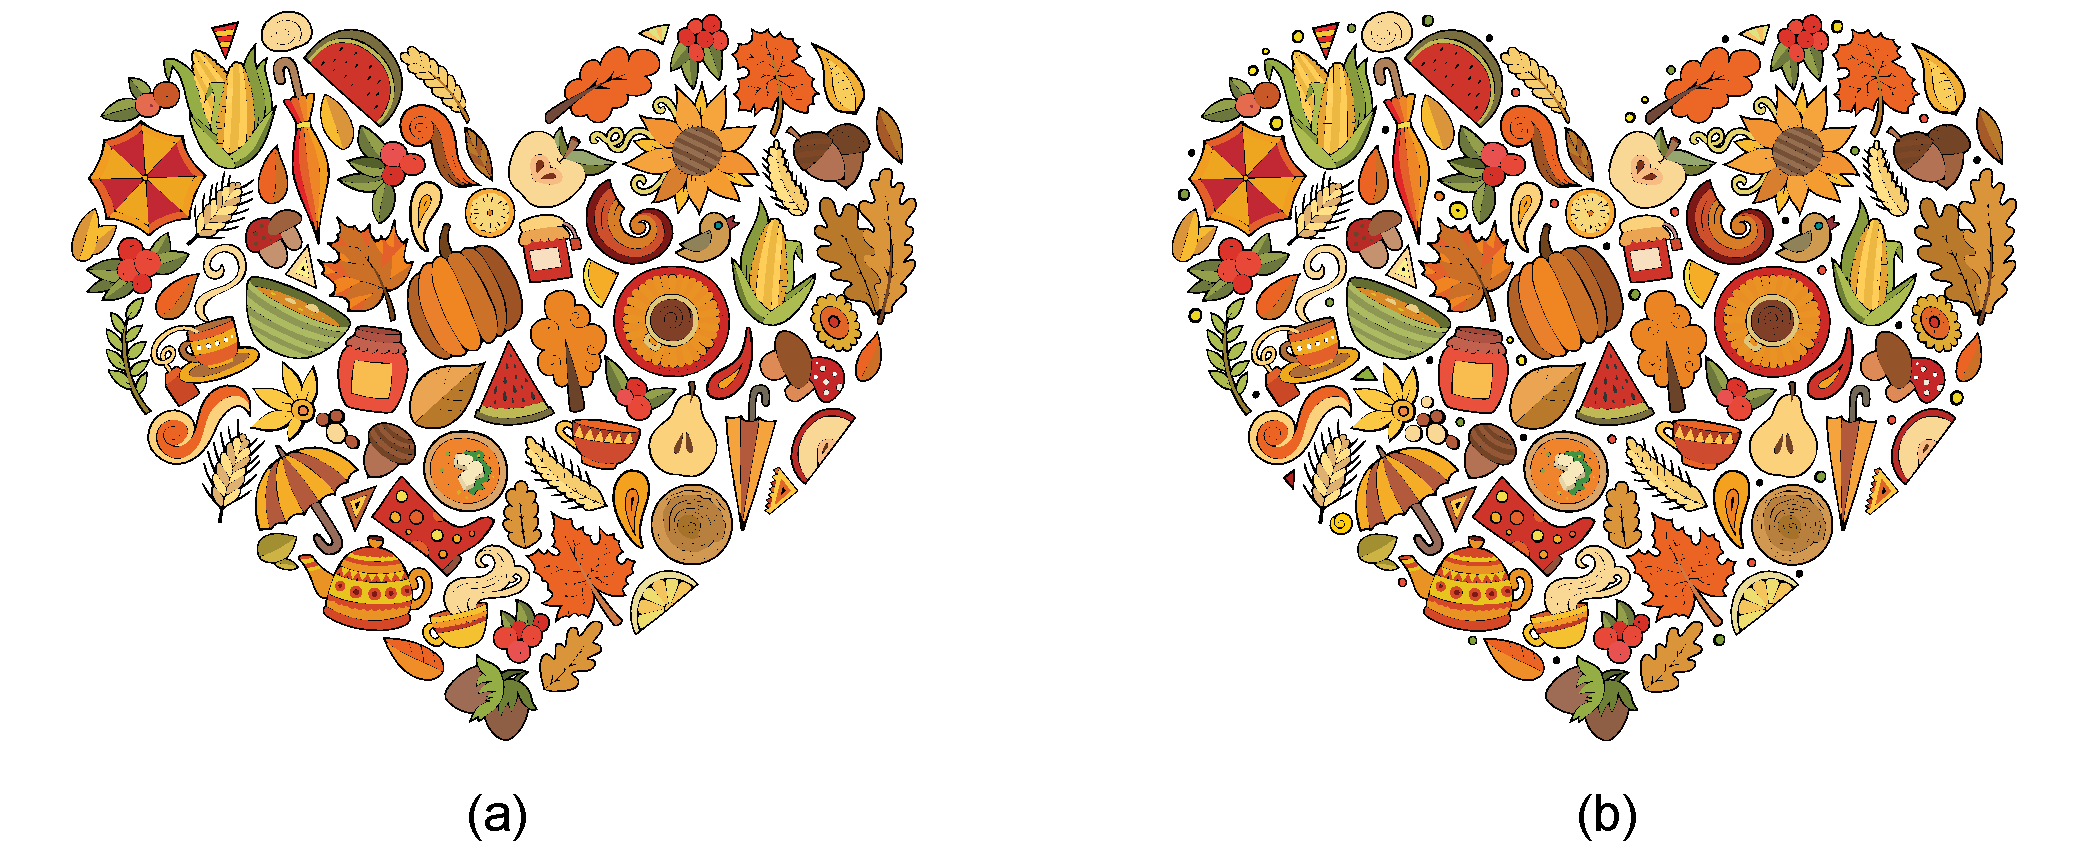
\includegraphics[width=1.0\textwidth]{figures/intro/primary_secondary.pdf}
\caption[Primary and secondary elements]{
  \label{fig_primary_secondary}
  \nnewtext
  {
  An autumn-themed packing created by Balabolka. }
  (a) The packing with primary elements only.
  (b) Secondary elements are added. 
}
\end{figure}

\begin{figure}[t]
\vspace{-20pt}
\centering
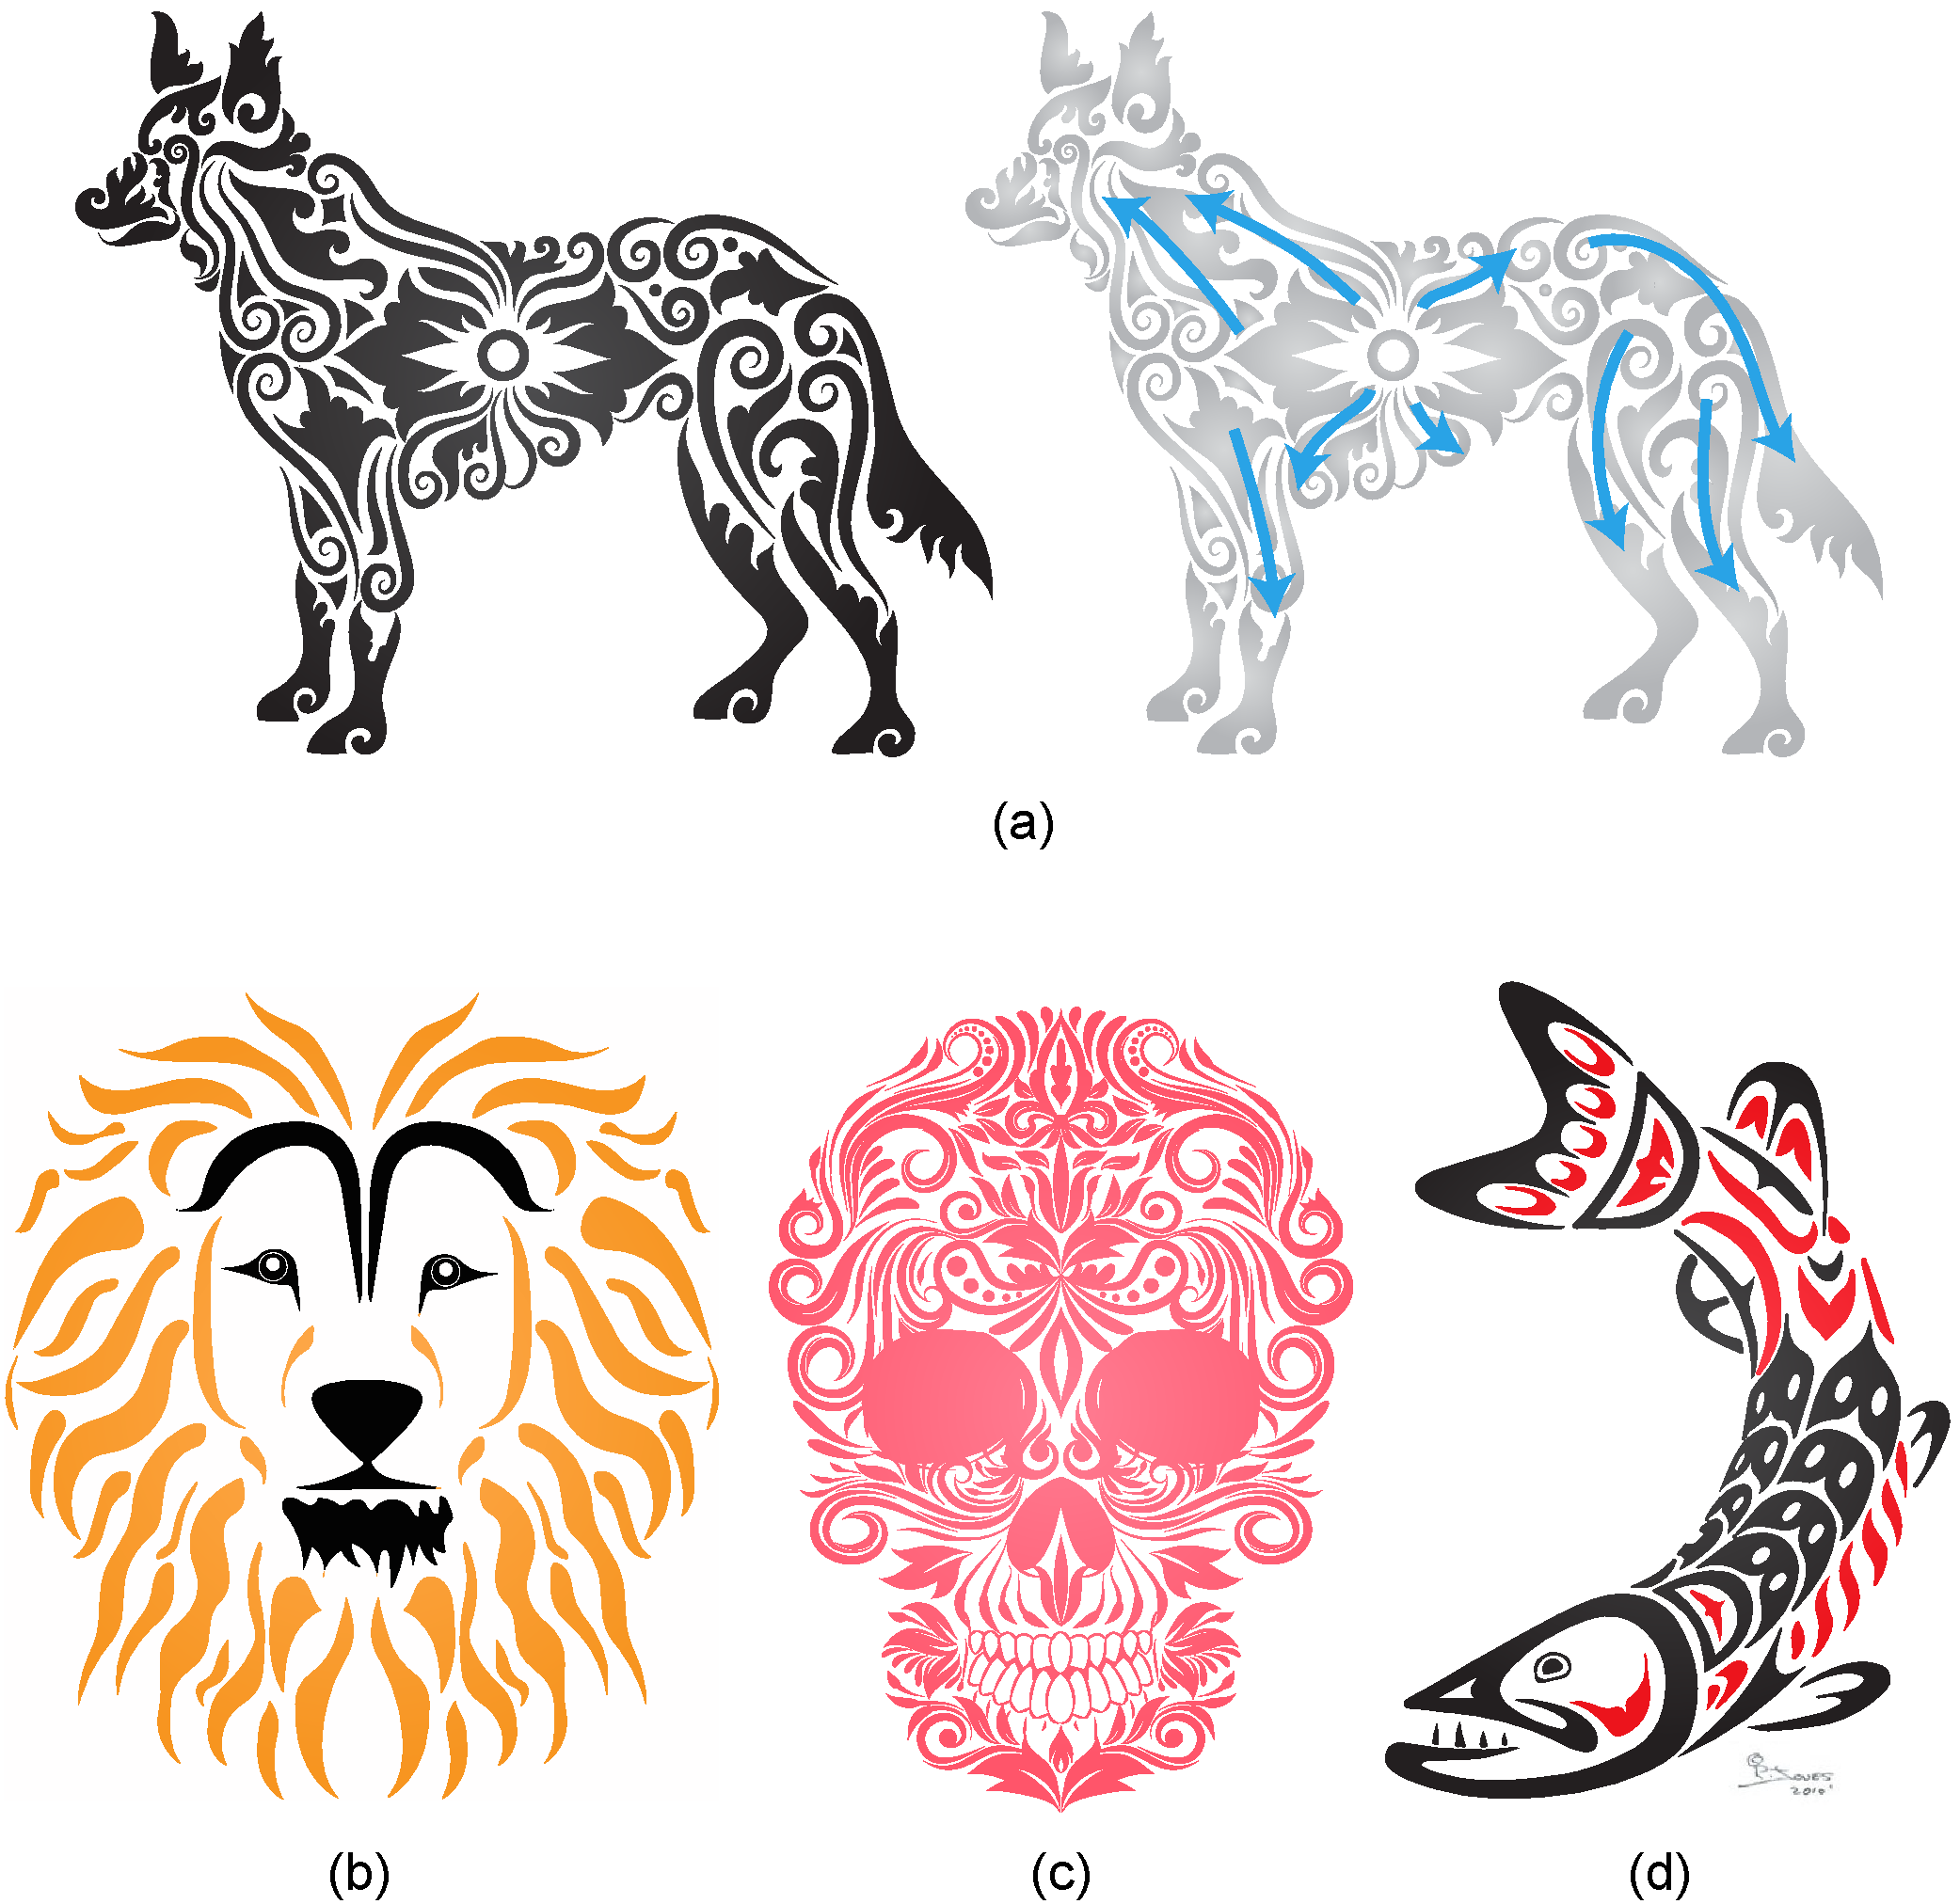
\includegraphics[width=1.0\textwidth]{figures/intro/dog_ornament_flow.pdf} 
\caption[Packings with flow visual styles]
{\label{fig_dog_flow} 
\nnewtext
{
Packings with flow visual styles:}
(a) Dog (by ComicVector703 on Shutterstock), 
including a visualization showing the flow directions of elements; 
(b) Lion (from StockUnlimited);  
(c) Skull (by alitdesign on Shutterstock).
(d) Fish in the style of Haida art (by Russ Jones, used with permission); 
 }
\end{figure}


%\begin{figure}
%\centering
%
\includegraphics[width=1.0\textwidth]{figures/intro/balabolka_dog_flow.pdf} 
%\caption[Packings in graphic design]
%{\label{fig_graphic_designs} 
%\newtext
%{
%Two packing examples in graphic design.
%(a) A packing of autumn-themed elements, created by Balabolka.
%(b) A packing of abstract-shaped elements that create a flow visual style, created by ComicVector703.
%}
% }
%\end{figure}

\begin{figure}
\centering
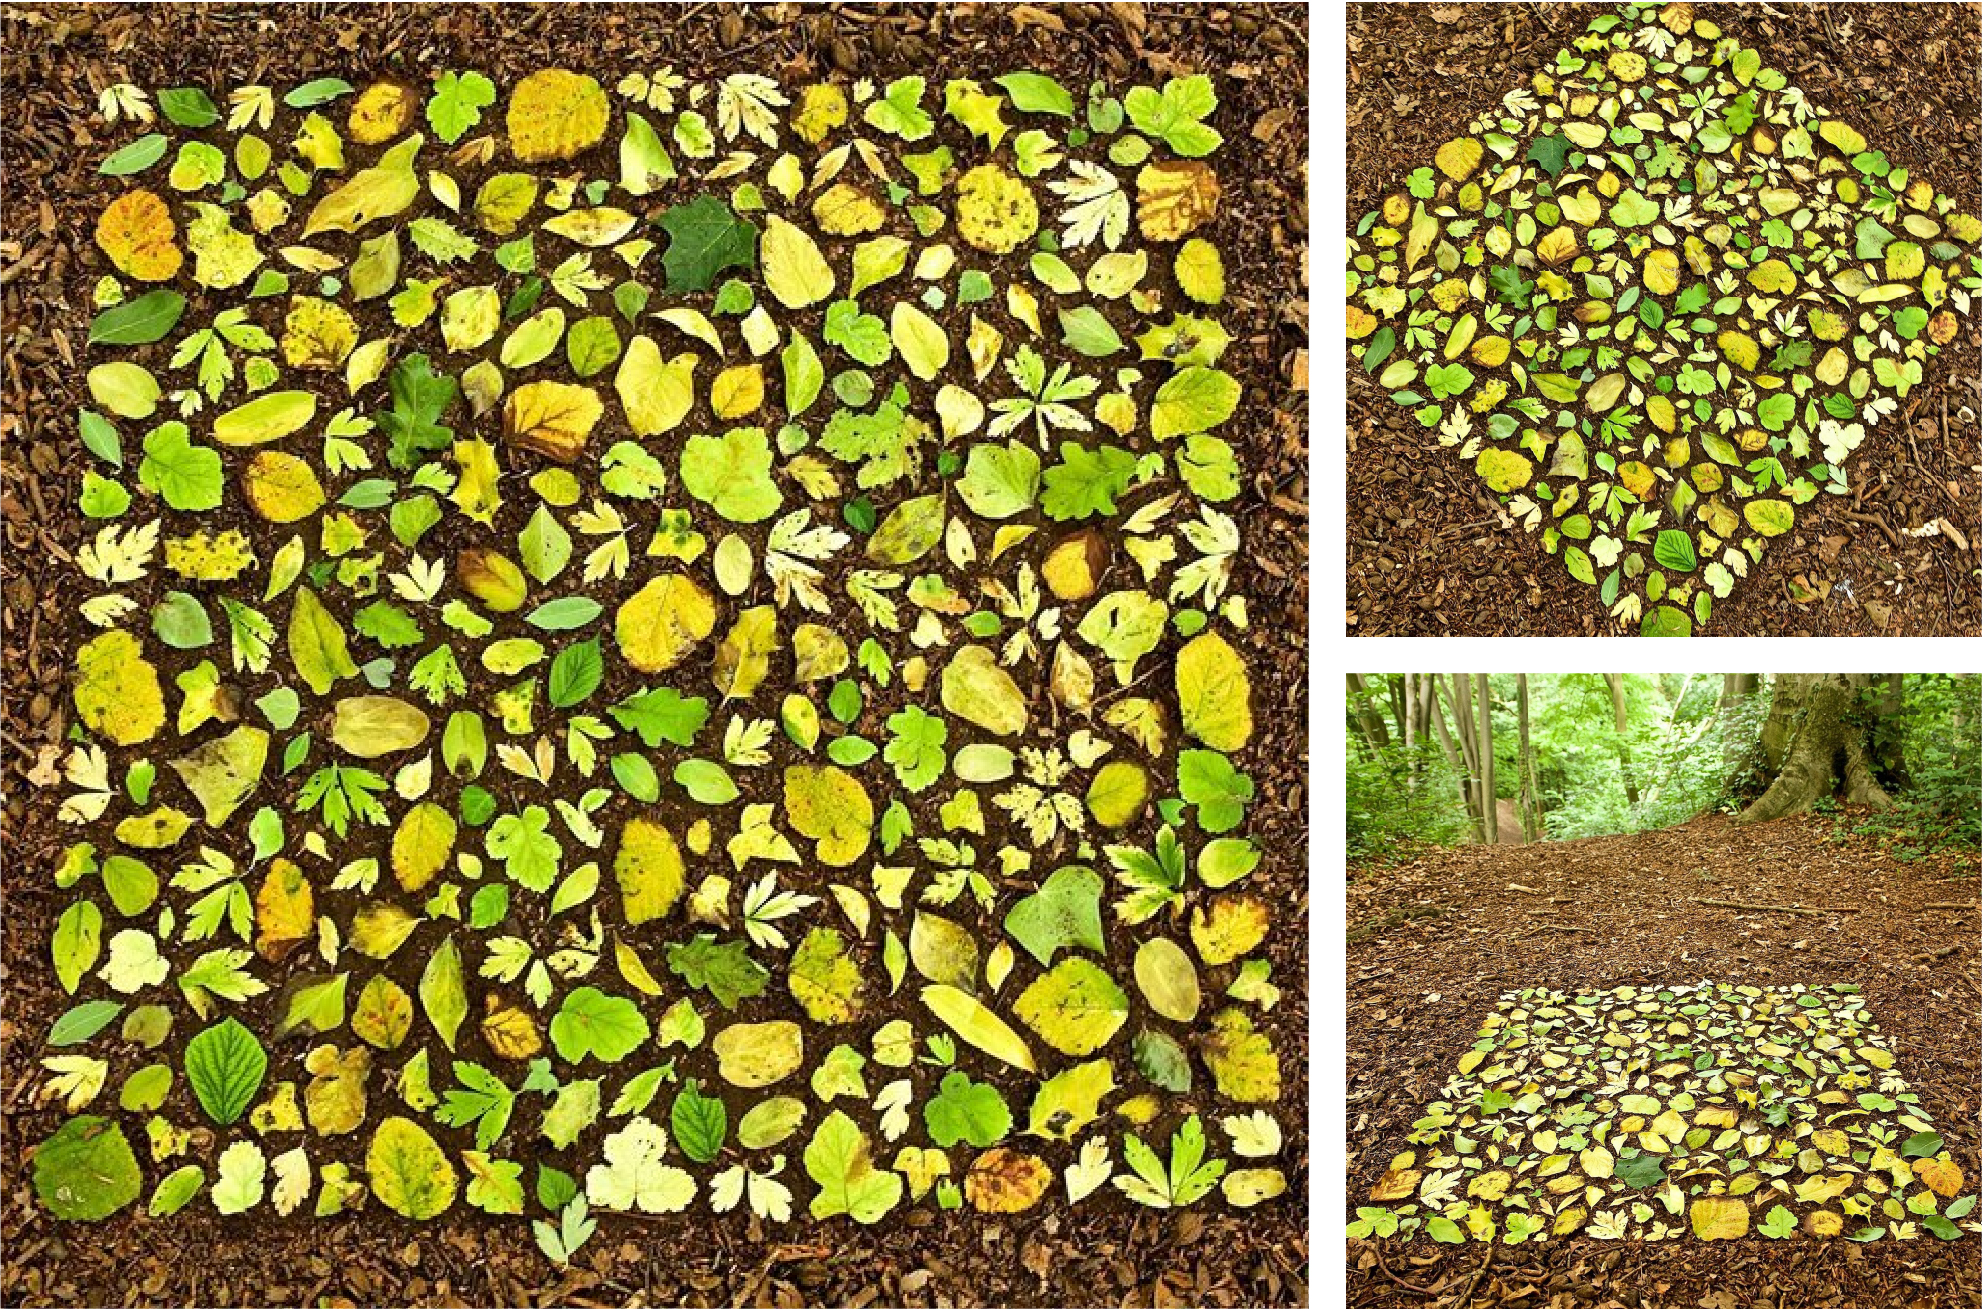
\includegraphics[width=1.0\textwidth]{figures/intro/woodland.jpg} 
\caption[A land art packing]
{\label{fig_woodland} 
\newtext
{
%A packing of leaves by James Brunt. 
A land art packing that is composed of leaves, created by James Brunt. 
Each leaf is oriented toward the center of the circle.
}
 }
\end{figure}

%\begin{figure}
%\centering
%\includegraphics[width=0.5\textwidth]{figures/intro/valve_lobby.jpg} 
%\caption{\label{fig_valve_lobby} 
%A packing installation in a lobby of a video game company. }
%\end{figure}

%\begin{figure}
%\centering
%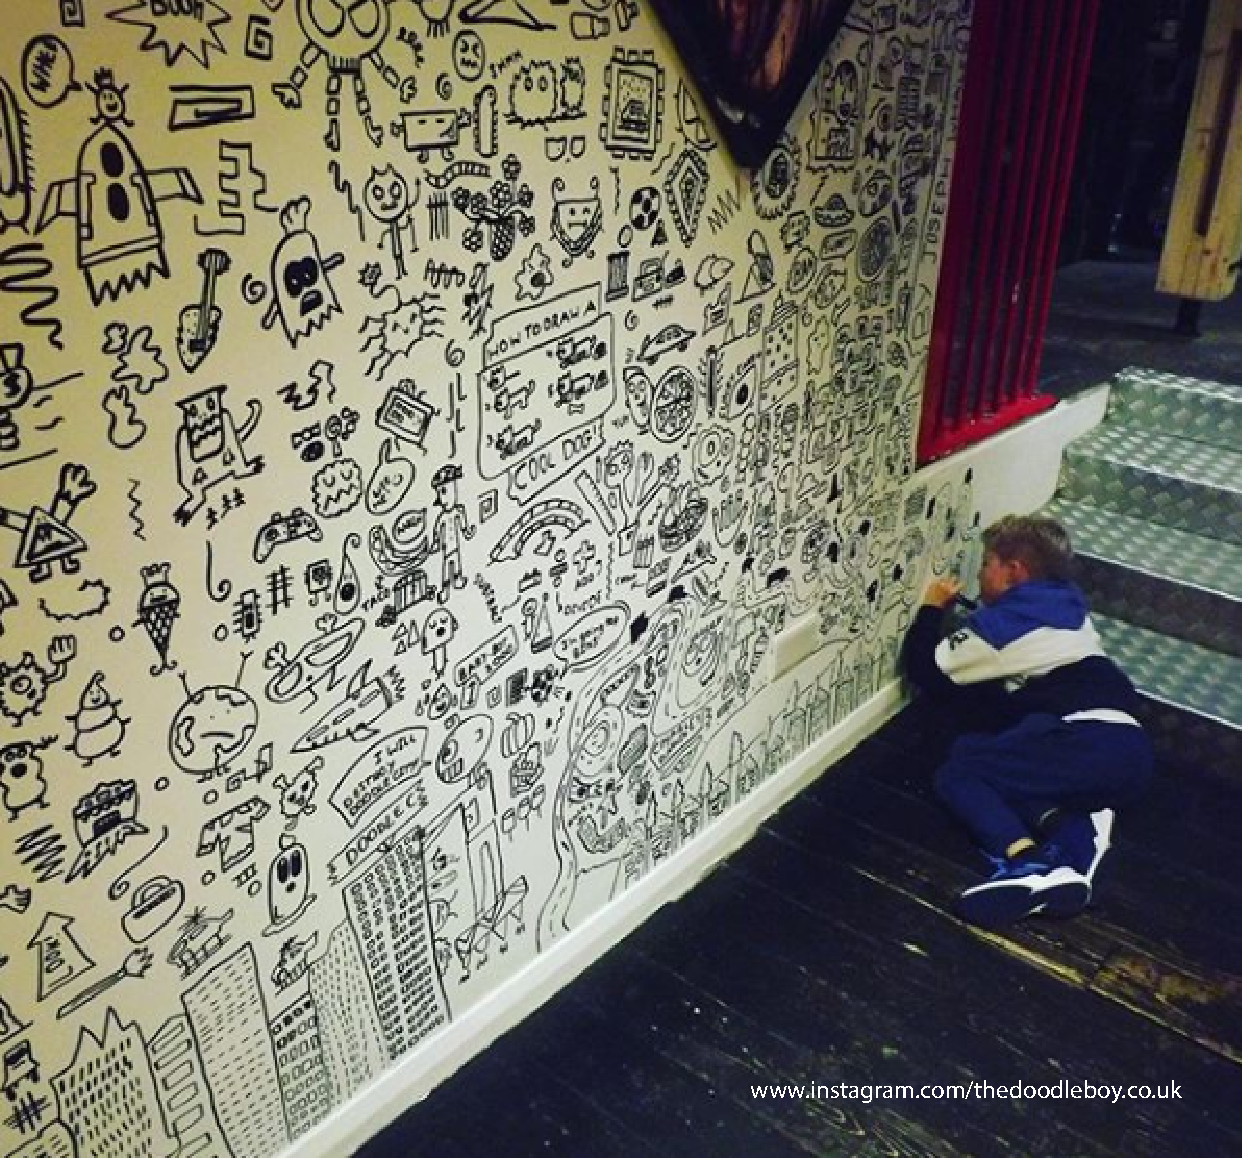
\includegraphics[width=0.5\textwidth]{figures/intro/doodle_boy.pdf} 
%\caption{\label{fig_doodle_boy} 
%Doodle boy. }
%\end{figure}

%\mynote{
%Thesis Statement (one or two sentences)
%\begin{packeditems}
%\item What is your thesis about and what have you done?
%\item If you have a hypothesis what is it?
%\item How will you test (prove/disprove) your hypothesis?
%\end{packeditems}
%}

%\mynote{align with boundary}

\newtext
{
A \textit{packing} is an arrangement of geometric
\textit{elements} within a \textit{container} region in the plane.
As an artistic composition, 
a packing can communicate a relationship between a whole and the parts that make it up.
Elements work together to communicate the overall container shape,
but each is large enough to be appreciated individually.
Elements are shapes like animals, plants, abstract geometry, or man-made objects.
Packings are popular in logo design, graphic design, and art.
Figure~\ref{fig_logo_packing}a shows the Unilever logo,
which is a 2D packing of elements arranged inside a U-shaped container.}


\newtext{The subset of the container that does not belong to any element is
called \textit{negative space} (Figure~\ref{fig_logo_packing}b).
We can also interpret negative space as separation and gaps between elements.}
\nnewtext{
On the other hand, elements can be interpreted as \textit{positive space}.
In this thesis, we narrow our focus in packings without element overlaps,
which makes it easier to discuss positive and negative space without 
``double counting'' the positive space.}

\nnewtext{The evenness of negative space plays an important role in packings.
Initially, an artist should arrange elements in a way that their boundaries interlock with each other,
causing the separation between neighboring elements to become roughly the same everywhere.
We refer those in the resulting packing as \textit{primary elements}.
However, the interlocking of primary elements is imperfect, so it is not uncommon that 
the artist artfully places smaller \textit{secondary elements} 
such as triangles or circles to reduce remaining large gaps,
see the autumn-themed packing in Figure~\ref{fig_primary_secondary}.}

 
%\newtext{Elements can also be oriented to follow certain directions for aesthetic reasons.
%Figure~\ref{fig_graphic_designs}b is an ornamental packing
%of long thin elements that are bent and oriented outward from the center of the torso to create a flow visual style.
%Another example is shown in Figure \ref{fig_woodland}, which is a packing of leaves, each is oriented toward the center of the container.
%On both examples, the flow visual style gives an impression of progression and movements.}
\nnewtext{
\textbf{Design Principles:}
In studying packing designs, 
we have identified five high-level principles that are important
to the construction of packings:
}
\begin{items}%[leftmargin=*]
\item \textbf{Balance.} A composition does not exhibit too
  much variation in local amounts of positive and negative space.
  Typically, this goal is accomplished by limiting variation in 
  the diameters of elements (controlling the variation in
  positive space), and in ensuring that elements are spaced 
  evenly (controlling negative space).
  \nnewtext{In Figure~\ref{fig_primary_secondary}, 
  the elements that build up the positive space, come in a variety of size but no one is too big to stand out. 
  Additionally, interlocking elements lead to gaps of negative space that are similar in width.}

\item \textbf{Flow.} In local parts of a composition, the elements
  are oriented to communicate a sense of directionality or flow.
  \nnewtext{All of the examples in Figure~\ref{fig_dog_flow} exhibit 
  some amount of flow.  In the dog, many elements appear to flow
  outward from the flower in the center of the torso, and then
  up the neck and down into the legs.  The scales and other elements
  on the fish flow along the length of its body.  In the lion and skull,
  elements flow horizontally outward from a central axis of symmetry,
  suggesting fur in the case of the lion.  
  Another example is shown in Figure \ref{fig_woodland}, which is a packing of leaves
  that are oriented toward the center of the container.}   
  Flow  adds visual interest to a composition, engaging the viewer 
  by providing a sense of progression and movement through elements.

\item \textbf{Uniformity Amidst Variety.} Repeated elements must balance
  between two opposing forces.  \textit{Uniformity} 
  aims for an overall unity of design; \textit{variety}
  seeks to break up the monotony of
  pure repetition.  Elements should be permitted to vary in shape,
  but in a controlled way.  We refer to this principle
  as \textit{uniformity amidst variety}, a term borrowed from 
  philosopher Francis Hutcheson~\cite{Hutcheson1729}.
  Gombrich also writes eloquently on the role of variation in 
  design~\cite{Gombrich}.
  \nnewtext{
  The Unilever packing in Figure~\ref{fig_logo_packing} has the elements drawn with a similar curvy style. 
  In Figure~\ref{fig_primary_secondary}, the elements are autumn-themed shapes and are convex or near convex. 
  In Figure~\ref{fig_dog_flow}, the dog's spirals and the
  fish's scales both obey this principle.  The lion and skull do as well,
  except that half of the elements are reflected copies of the other
  half, across a vertical line through the center of the composition.
  This repetition emphasizes the bilateral symmetry in the design.
  The land art packing in Figure~\ref{fig_woodland} have the most uniformity than the other examples
  since the leaves have a similar shape and the composition conveys the radial symmetry, 
  however, the artist added some amount of variety by using different leaf sizes and colors.
  }

\item \textbf{Fixed Elements.} Compositions use a small number of fixed
  elements to solve specific design problems or provide focal points.
  In any figurative drawing, eyes serve as a powerful focal point;
  every example in Figure~\ref{fig_dog_flow} has eyes drawn
  in as unique elements
  (the dog's eye is expressed via a carefully placed spiral).  Other
  situations that call for specialized shapes include the dog's paws,
  the fish's teeth and fins, 
  the lion's eyes and nose, %%% REZA BACKUP
  and the skull's teeth.
  Sharp variation in the balance of positive and negative space
  can also be used to emphasize a focal point,
  as in the fish's head and the lion's face that contain considerable amount of empty space.

\item \textbf{Boundaries.} In many ornamental packings, elements are
  carefully arranged to conform to and emphasize container boundaries.
  The fish demonstrates this principle most clearly: we can easily
  fill in the gaps between elements to form a mental image of a continuous
  outline.  The dog's elements are also well aligned to indicate the
  container shape.  However, this rule is not universal.  
  The lion artfully subverts it with elements that flow outward to an
  indistinct boundary, helping to convey the appearance of fur.
\end{items}


\textbf{Previous Methods:} \newtext{There has been a moderate amount of past research in computer
graphics, particularly in the field of non-photorealistic rendering,
on the generation of packings, or mosaics.  
See Chapter~\ref{chapter_related_work} for specific examples.  
However,  most techniques pack elements via rigid transformations, leading to
uneven element distribution and overlaps.  
Jigsaw Image Mosaics~\cite{Kim2002} and collages based on the Pyramid of Arclength
Descriptor~\cite{Kwan2016} are \textit{data-driven}.
These techniques rely on a large library of elements, so that given an
area to fill in a partial composition, there is likely to be an
element in the library with a compatible shape.  The challenge is 
\textit{finding compatible elements},
which requires designing a shape matching technique that is fast and robust.
Additionally, they cannot guarantee to find a compatible element
at every iteration, and elements typically do not fit perfectly with each other 
or the container boundary.
The remedy here is providing more data with increased computation time.
However, a large library may not be feasible or artistically desirable.
If an artist wants a packing of hand-drawn cats, and a data-driven approach 
cannot find a good result with ten cat shapes, 
the artist may not want to draw 100 or 1000 cats to ensure a better fit.
}

\textbf{Deformation-Driven Methods:} \newtext{In this thesis, we propose \textit{deformation-driven} methods.
Instead of finding compatible elements,
we \textit{create} compatible elements through deformation; 
these deformed elements can adapt to the shapes of neighboring elements and the container boundary.
We allow elements to deform in a controlled way,
to trade off between the evenness of the element distribution and 
the deformations of the individual elements.
By building an algorithm with a controllable deformation model at its core, we achieve a
more even distribution of negative space, 
and we require only a small library of element shapes.}
\nnewtext{
Deformation-driven methods also allow us to work toward the principle of uniformity amidst variety.
We can achieve a degree of uniformity by using repeated copies of a small library of elements, but balance that uniformity with
variety by deforming those elements. 
We believe that there is a value in deformation that can generate plausible families of related elements from a single input shape.
}

%\newtext
%{
%Deformation-driven methods also allow us to work toward a design principle called \textit{uniformity amidst variety}~\cite{Hutcheson1729, Gombrich}. 
%\textit{Uniformity} aims for an overall unity of design and 
%\textit{variety} seeks to break up the monotony of pure repetition.
%We can achieve a degree of uniformity by using repeated copies of a small library of elements, but balance that uniformity with
%variety by deforming those elements. 
%We believe that there is a value in deformation that can generate plausible families of related elements from a single input shape.
%}

\nnewtext{
In this thesis, we develop many techniques that are inspired by physical simulations.
We have to create an element representation 
that can be deformed by pseudo-physical forces. 
Even though we do not contribute to a new physically-based technique,
we treat a physical simulation as an optimization process that allows us to
reach a physical equilibrium where the resulting packing has approximately uniform
distribution of both positive and negative space.
}

\newtext
{
% https://learningenglish.voanews.com/a/the-more-i-practice-the-more-i-remember/4995040.html
The perceived packing quality is closely tied to the evenness of negative space.
The more the elements interlock, the more even the negative space. 
We are interested in quantitative measurements of evenness 
in order to evaluate and compare packing algorithms.
In this thesis we discuss several possible measurements of 
evenness based on methods from spatial statistics.
}

\textbf{Contributions:} \newtext
{
In this thesis, we develop three specific deformation-driven packing methods, 
and then study investigate the quantitative evaluation of packing quality in greater detail:
\begin{enumerate}
\item FLOWPAK is a packing method that deforms long thin elements to follow a user-defined vector field (Chapter~\ref{chapter_flowpak}).
\item RepulsionPak is a packing method that utilizes repulsion forces to distribute and deform elements,
	each is represented as a mass-spring system (Chapter~\ref{chapter_repulsionpak}).
\item AnimationPak is a method to pack 2D animated elements inside a static 2D container. 
	Each element is an extruded 3D shape in a spacetime domain 
	and we view the animated packing problem as a 3D packing in that domain.
	(Chapter~\ref{chapter_animationpak}). 
\item  Quantitative metrics for measuring the evenness of negative space: spherical contact probabilities,
histograms of the distance transforms, and the overlap functions (Chapter~\ref{chapter_qualitative_metrics}). 
\end{enumerate}
}

%\begin{labeling}{alligator}
%\item [ant] really busy all the time
%\item [chimp] likes bananas
%\item [alligator] very dangerous animal, sharp teeth, long
%muscular tail and a bit of text that is longer than one
%line and shows the alignment of text quite nicely
%\end{labeling}


%\mynote{TODO: Copy from comp\_2}
%A \textit{packing} is an arrangement of 2D geometric
%\textit{elements} within a \textit{container} region in the plane.
%Packings are popular in art, ornamentation, and graphics design.
%Figure ~\ref{fig_logo_packings}\ref{fig_graphics_designs}\ref{fig_woodland}\ref{fig_valve_lobby}\ref{fig_doodle_boy} show several packing examples.
%They can effectively convey a relationship between a unified whole (the
%container shape) and its many sub-parts (the elements).

%\mynote{maybe put negative space to the background section}
%Elements are shapes like animals,
%plants, geometric forms, or man-made objects.
%An artist distributes elements so that they communicate
%the shape of the container. 
%The subset of the container that does not belong to any element is
%called \textit{negative space}
%(Fig.~\ref{packing_example}, right).
%We can also interpret negative space as separation and gaps between elements.
%The evenness of negative space plays an important role in 
%packings.  
%The artist should arrange elements in a way that their boundaries interlock with each other,
%causing the separation between neighbouring elements to become roughly the same everywhere.
%As the elements in a packing become perfectly interlocked,
%the packing turns into a \textit{tiling}: a set of elements that exactly
%fill a container with no overlaps and no negative space (Fig.~\ref{related_work_images}b).



%\mynote{Motivation, Why is this problem you've worked on important}
%\mynote{Goals / Objectives, What are you trying to do and why? 
%How will you or the reader know if or when you've met your objectives?}


%\mynote{
%Contributions, What is new, different, better, significant? Why is the world a better place because of what you've done? What have you contributed to the field of research?  What is now known/possible/better because of your thesis?
%}



%\mynote {Explain briefly FLOWPAK, RepulsionPak, and AnimationPak.}

%%%%%%%%%%%%%%%%%%%%%%%%%%%%%%%%%%%%%%%%%%%%%%%%%%%%%%%%%%
\chapter{Related Work}
\label{chapter_related_work}
%%%%%%%%%%%%%%%%%%%%%%%%%%%%%%%%%%%%%%%%%%%%%%%%%%%%%%%%%%

\begin{figure}[t]
\centering
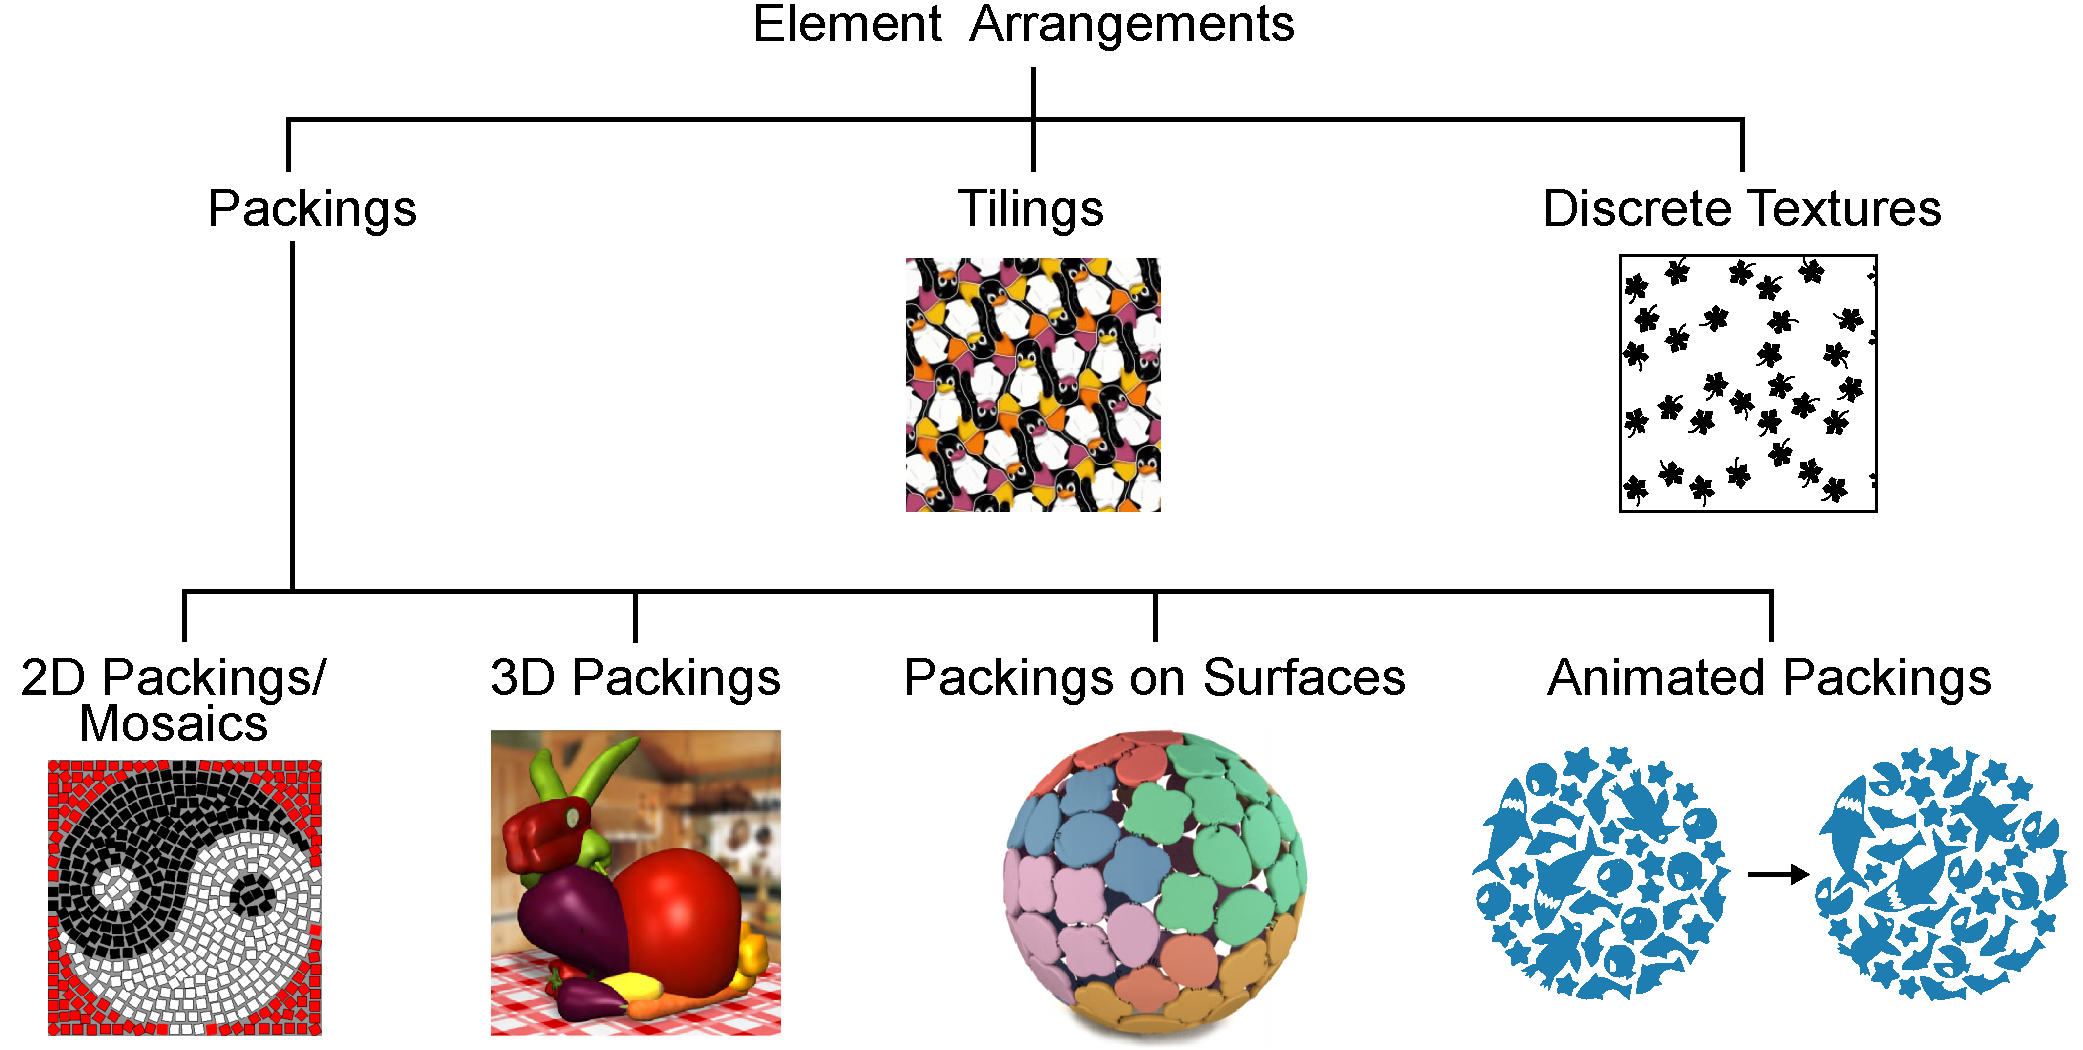
\includegraphics[width=1.0\textwidth]{figures/related/taxonomy.pdf} 
\caption[A categorization of element arrangements]
{\label{fig_taxonomy} 
\newtext
{
A simplified categorization of element arrangements.
}
}
\end{figure}


\begin{figure}
\centering
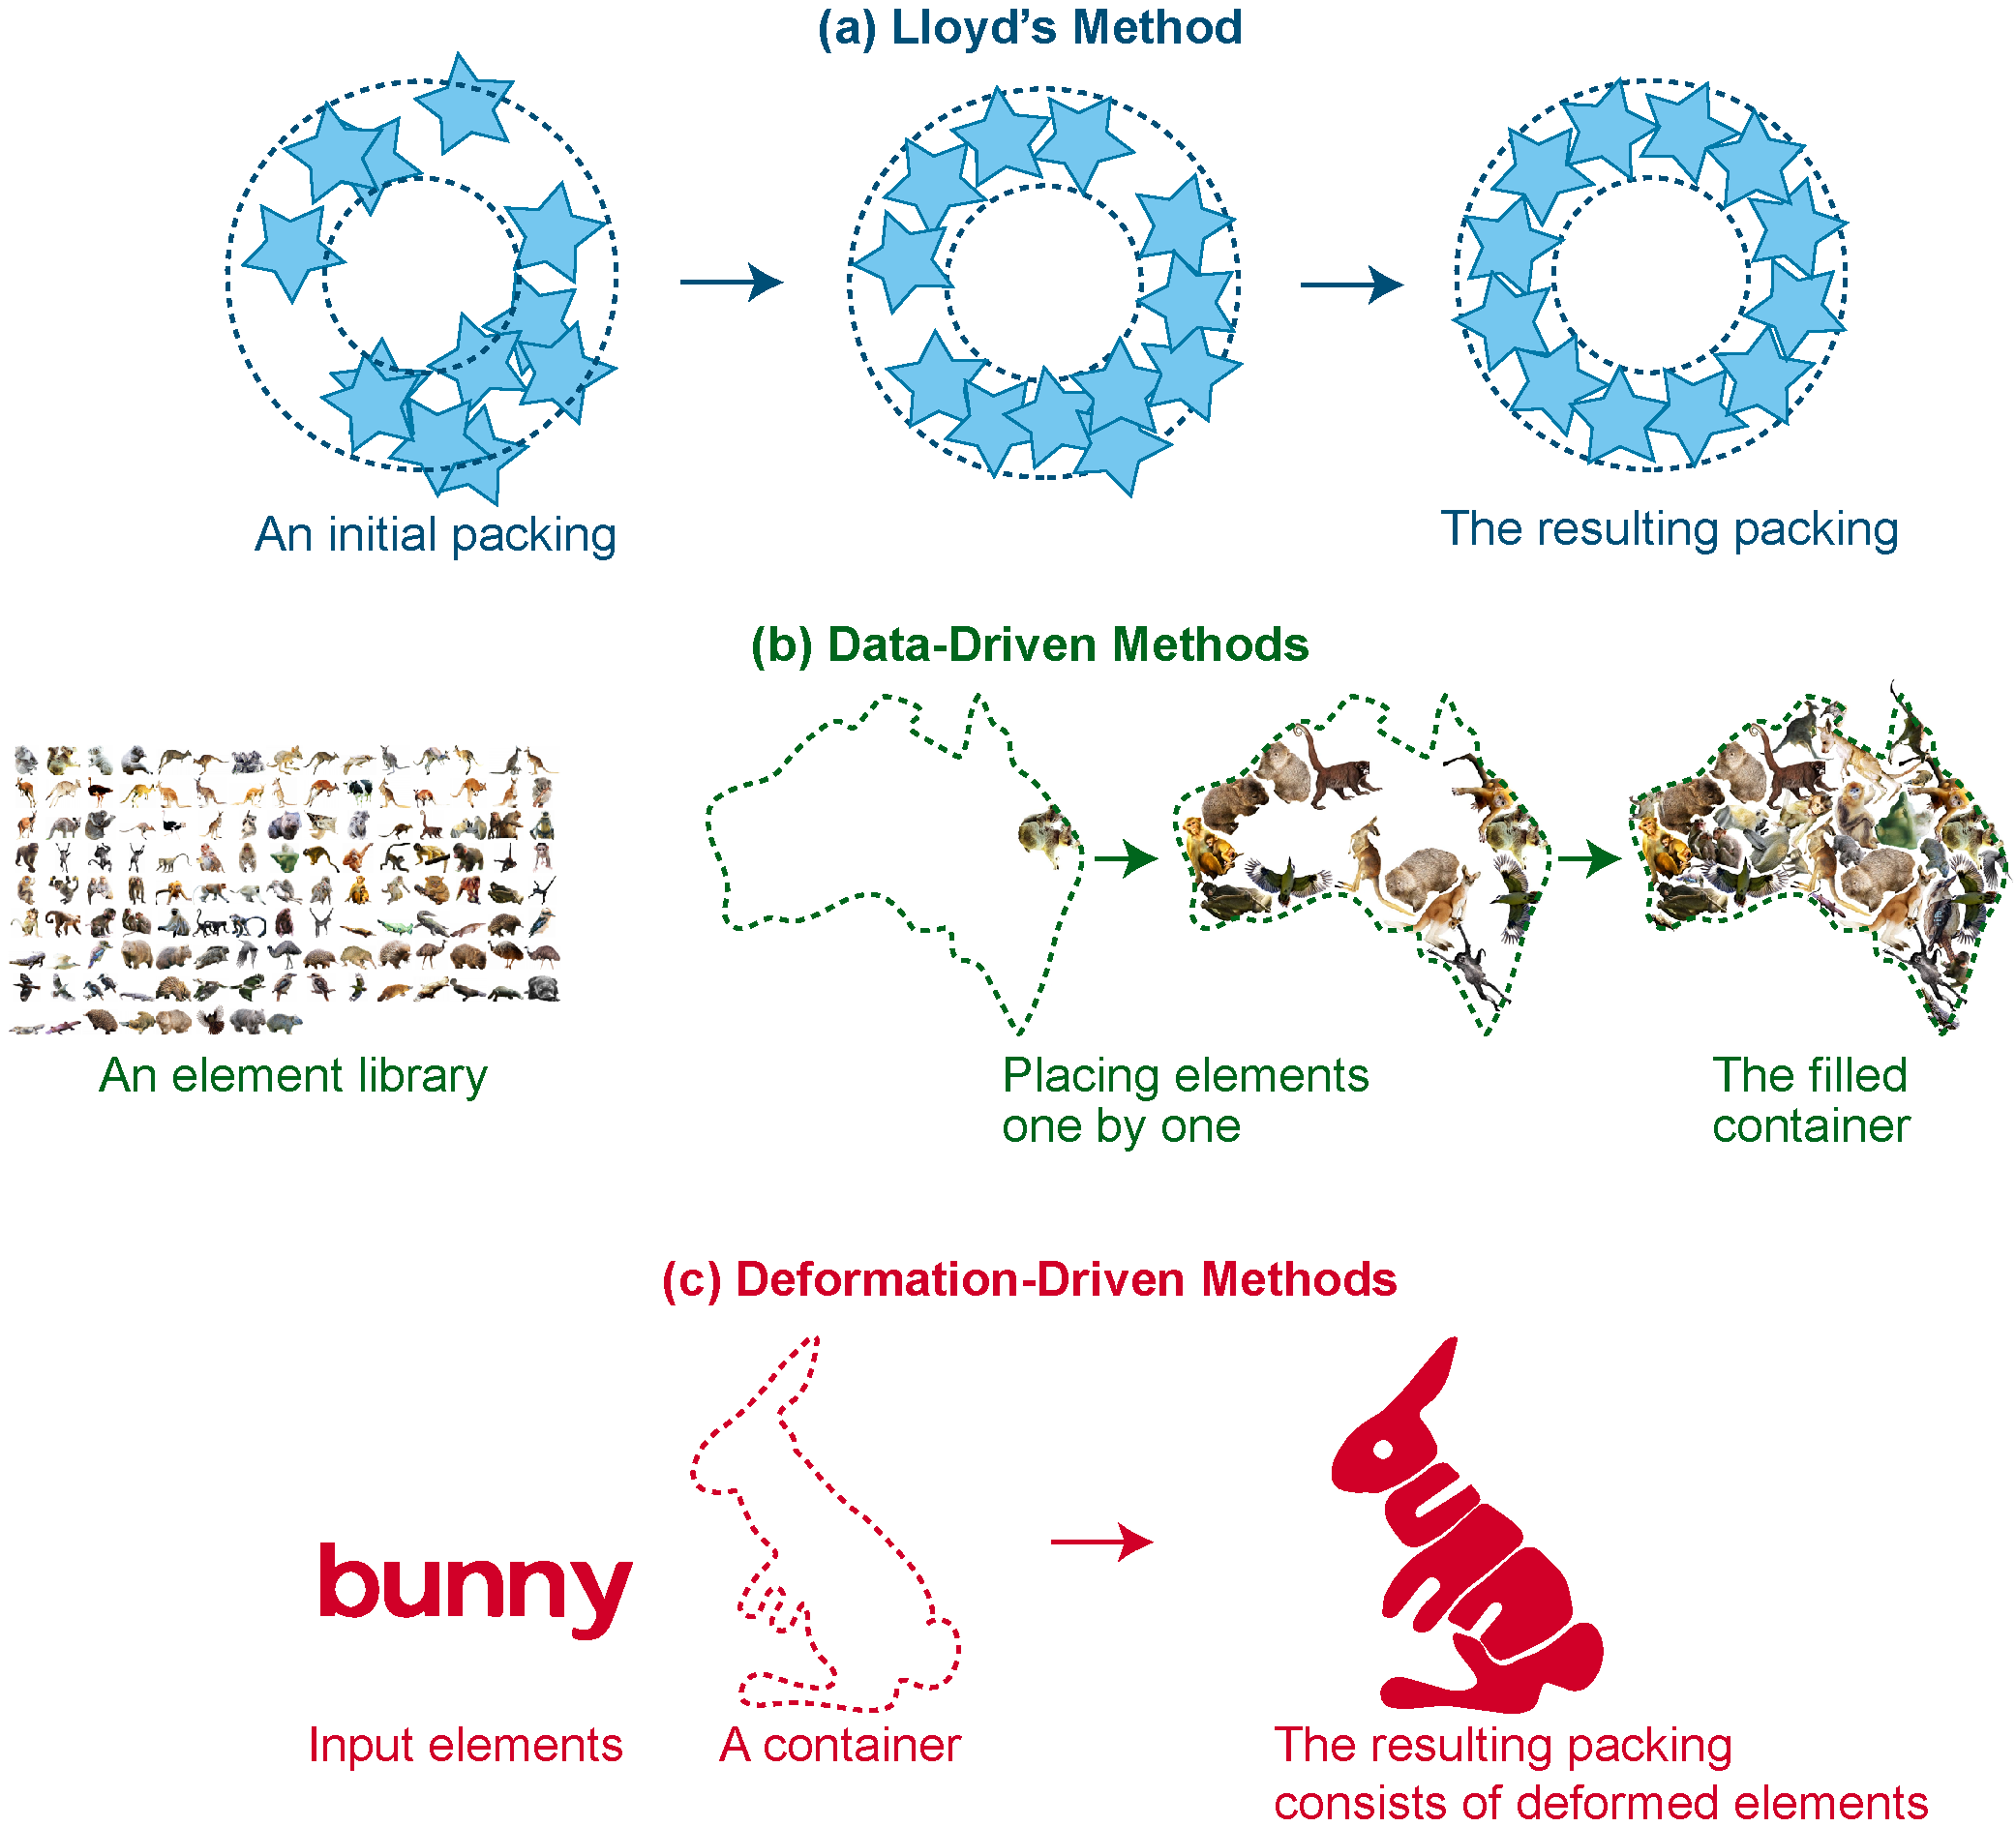
\includegraphics[width=1.0\textwidth]{figures/related/taxonomy_method.pdf} 
\caption[Three popular methods in mosaicing and packings]
{\label{fig_taxonomy_method} 
\newtext
{
Three popular methods in mosaicing and packings.
%Many mosaicing and packing methods can be grouped into three categories. 
(a) Lloyd's method starts with an initial distribution of elements then iteratively \nnewtext{displaces} them
to generate a more even packing. 
(b) A data-driven method places elements one by one until the container is filled.
For each step, it \nnewtext{selects} an element from an element library that is compatible with already placed elements and the container.
(c) A deformation-driven method attempts to create element compatibility through deformation.
The illustrations are adapted from \nnewtext{The Spectral Approach~\cite{Dalal2006}, 
Pyramid of Arclength Descriptors~\cite{Kwan2016}, and
Legible Compact Calligrams~\cite{Zou2016}}.
}
}
\end{figure}

\newtext
{
An element arrangement is defined as a distribution of non-overlapping elements in the plane.
Decades of research in NPR have produced many techniques for producing computer-generated element arrangements.
Based on their designs, categories of elements arrangements include
packings, tilings, and discrete textures (Figure~\ref{fig_taxonomy}).
The categorization can be further expanded but we only choose ones that are related to this thesis.
We further break down the packing category into several subcategories: mosaics, 2D packings, 3D packings, 
packings on surfaces, and animated packings.
\nnewtext{This chapter covers the entire categorization except animated packings, which} are discussed in Chapter~\ref{chapter_animationpak}. 
%Many packing methods discussed in this chapter aim to minimize element overlaps, and
%a few computer-generated packings shown in this chapter 
%contain overlaps to some degree due to the challenge of finding and aligning compatible elements.
Most packing techniques have the goal to generate overlap-free packings, but in reality, it is a difficult task.
A few computer-generated packings shown in this chapter 
contain overlaps to some degree due to the challenge of finding and aligning compatible elements.
}

\newtext
{
\nnewtext
{Many packing algorithms can also be grouped according to their main algorithmic techniques} (Figure~\ref{fig_taxonomy_method}).
The first category, Lloyd's method, iteratively refines an initial element arrangement to generate a more even distribution.
The second category, data-driven methods, places elements one by one. For each step,
an element is taken from an element library that is compatible with previously placed elements and the container boundary.
The last category, deformation-driven methods, attempts to create element compatibilities through shape deformation.
}

%%%%%%%%%%%%%%%%%%%%%%%%%%%%%%%%%%%%%%%%%%%%%%%%%%%%%%%%%%
\section{Mosaics}
%%%%%%%%%%%%%%%%%%%%%%%%%%%%%%%%%%%%%%%%%%%%%%%%%%%%%%%%%%
\newtext
{
Mosaics are 2D arrangements that are popular for decorating floors or walls.
In traditional mosaics, elements are made of stone, ceramics, or glass.
The majority of these mosaicing techniques use \nnewtext{Lloyd's} method to distribute elements
via rigid transformations (Figure~\ref{fig_taxonomy_method}a).
Originally, Lloyd's method \nnewtext{was introduced in computer graphics} by \mbox{McCool} and Fiume to distribute point elements~\cite{McCool1992}.
\nnewtext{It was later} generalized to distribute convex and concave elements.
}

\newtext
{
We first discuss the simplest variant of Lloyd's method that distributes point elements, 
as shown in Figure~\ref{fig_lloyds_method}.}
\newtext{Given $N$ point elements, we first compute a \textit{Voronoi diagram} that partitions the plane into $N$ regions such that
all points inside a Voronoi cell are closest to its associated point element.
Lloyd's method moves every point element to the centroid of its Voronoi cell, 
then the Voronoi diagram is recomputed.
The process is repeated until the distribution is even,
\nnewtext{meaning that} the point elements are located at the centroids of the Voronoi cells.
The final structure is called a \textit{centroidal Voronoi diagram} (CVD).
}

\newtext{When computing centroids, a standard CVD assumes the area density is uniform everywhere.}
\newtext{Secord~\cite{Secord2002} computed a weighted CVD so that the resulting point element distribution
resembles a stippling artwork (Figure~\ref{fig_related_secord_hausner}a).}
\newtext{His method incorporates the pixel intensities of an input image to construct \nnewtext{a density function}. 
This alters the centroid calculation so that point elements are attracted to \nnewtext{darker regions}.}

\newtext{A standard CVD is generated using Euclidean distance, but other metrics lead to different shapes of Voronoi cells.
Hausner~\cite{Hausner2001}} \newtext{simulated the appearance of traditional mosaics by using} 
\newtext{Manhattan distance, producing Voronoi cells that resemble squares instead of hexagons.
Each Voronoi cell is then replaced with a square element and the resulting arrangement
resembles the appearance of traditional mosaics (Figure~\ref{fig_related_secord_hausner}b). 
However, a standard CVD computes only the positions of the square elements, and Hausner must
incorporated a vector field to modify the orientation of the metric
and rotate the square elements. 
Additionally, the approach is only suitable for square elements as
more complicated shapes, such as long rectangles, would have severe overlaps.}
\newtext{More recently, Doyle et al.~\cite{Doyle2019} and Javid et al.~\cite{Javid2019} generated pebble mosaics 
using a superpixel image segmentation~\cite{Achanta2012}, which is a variant \nnewtext{of} Lloyd's method that \nnewtext{blends an} Euclidean metric \nnewtext{with} a CIELAB colour metric.
They later elongated the Voronoi cells to follow the gradient of the input image, 
and smoothed out the cell boundaries. 
The resulting Voronoi cells resemble smooth elongated pebble shapes.
}

\begin{figure}
\centering
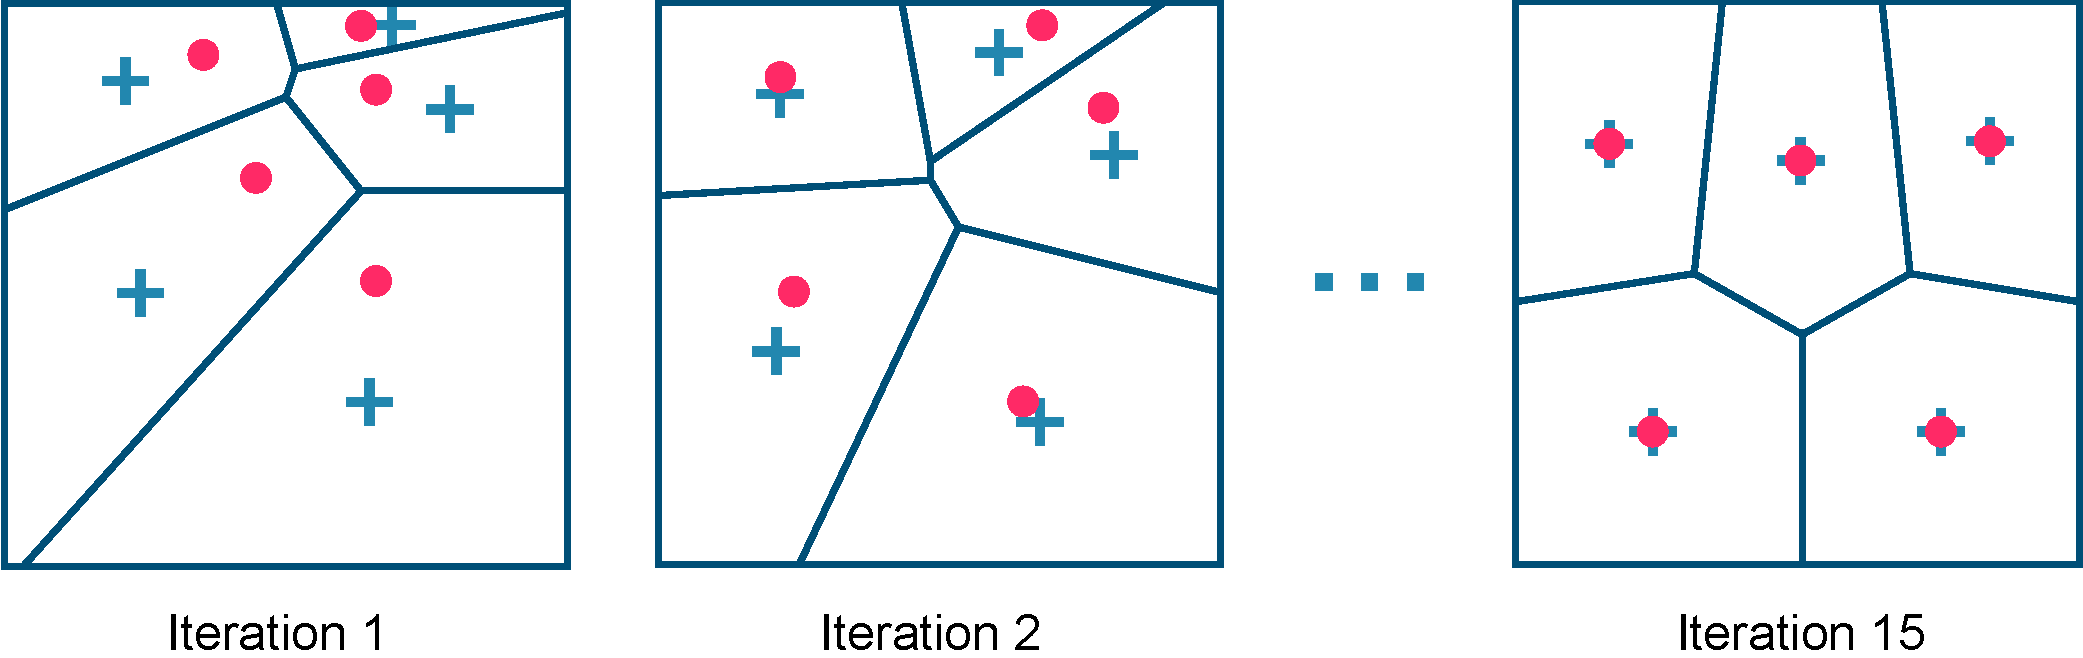
\includegraphics[width=1.0\textwidth]{figures/related/lloyds_method.pdf} 
\caption[An illustration of Lloyd's method.]
{\label{fig_lloyds_method} 
\newtext
{
An illustration of point-based Lloyd's method.
A Voronoi diagram is generated from the input point elements (drawn as red dots).
We then move the point elements to the centroids of Voronoi cells (drawn as plus signs).
The process is repeated until convergence, producing a centroidal Voronoi diagram.
Figure source is Wikipedia, drawn by Dominik Moritz under CC0 1.0.
}
}
\end{figure}


\begin{figure}
\centering
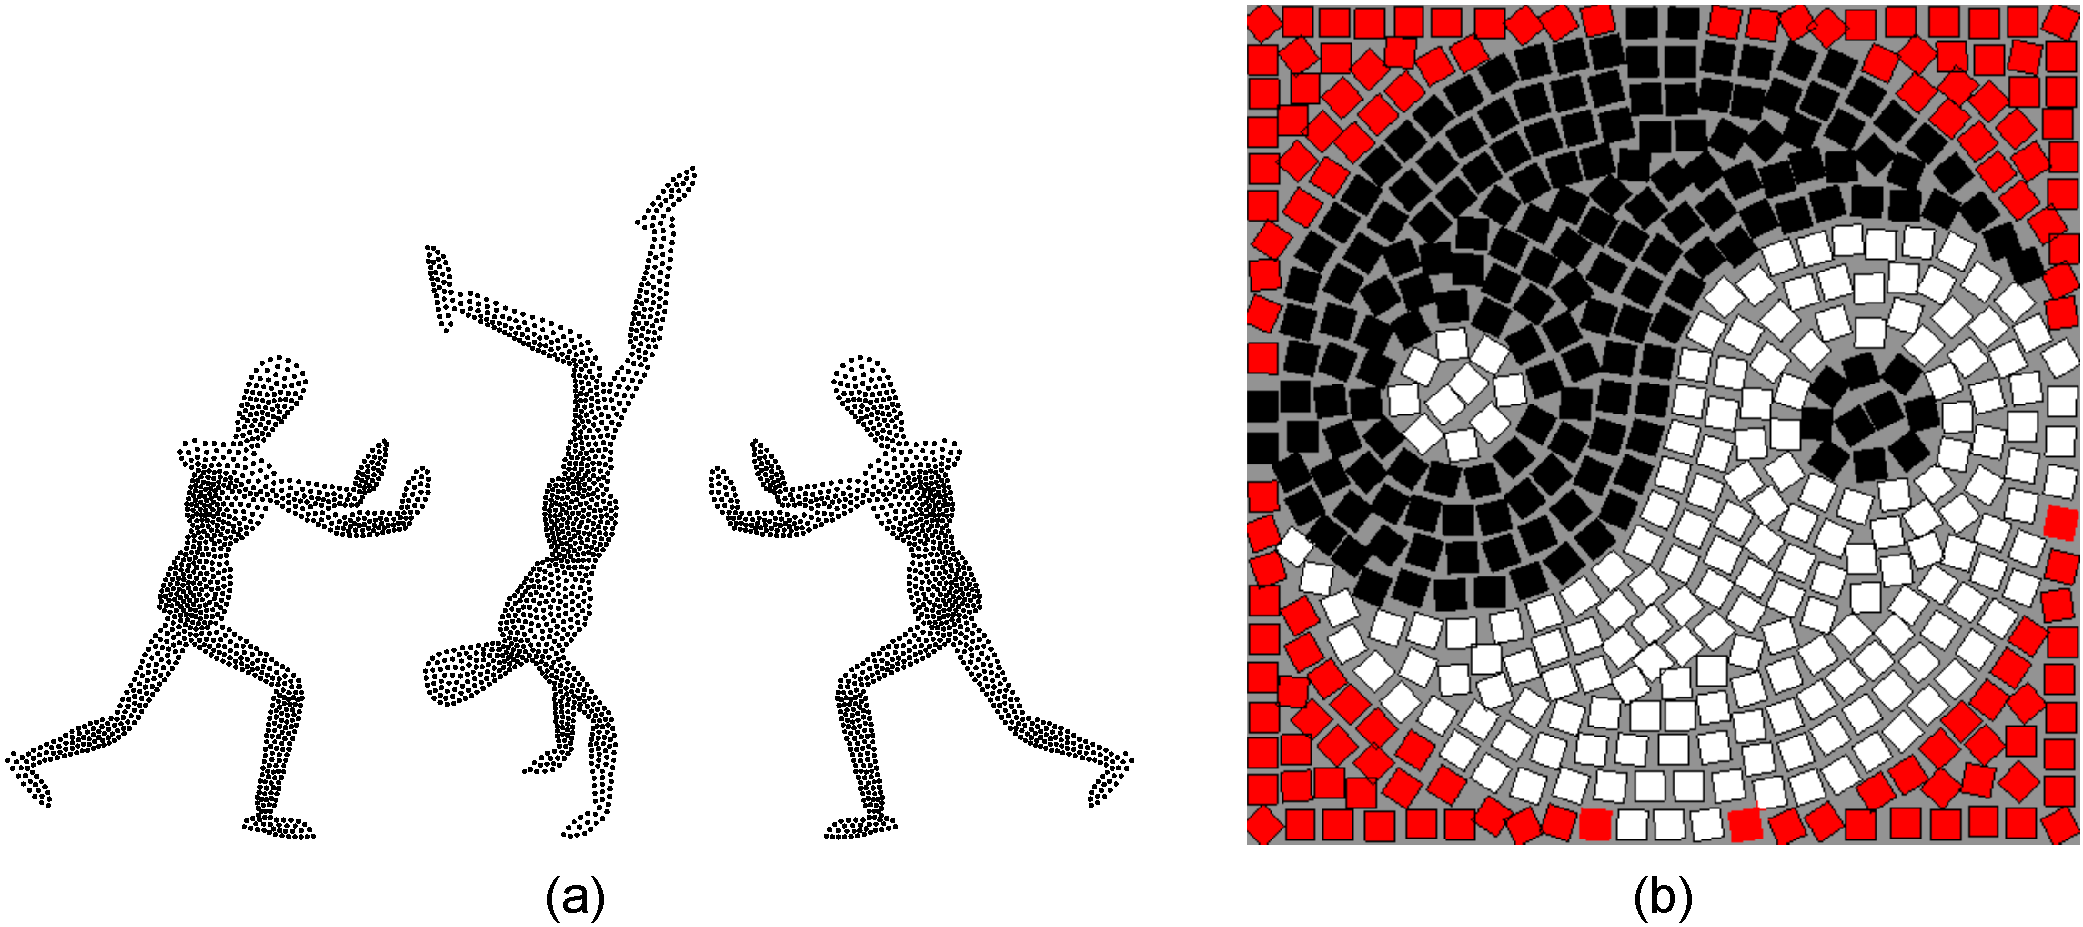
\includegraphics[width=1.0\textwidth]{figures/related/secord_hausner.pdf} 
\caption[Stippling artwork and traditional mosaics]
{\label{fig_related_secord_hausner} 
\newtext
{
(a) Stippling artwork of point elements generated using Lloyd's method 
that incorporates pixel densities of the input image~\cite{Secord2002}.
(b) Mosaics of square elements generated using Lloyd's method with Manhattan distance~\cite{Hausner2001}
}
}
\end{figure}

\newtext{We now discuss the computation of Voronoi diagrams that is generalized 
to any shapes for which a distance measurement exists.} 
\newtext
{Hiller et al.~\cite{Hiller2003} extended Lloyd's method to construct \textit{centroidal area Voronoi diagrams} (CAVDs),
a variant of CVDs that \nnewtext{yields} a distribution of polygonal elements.
This new extension computes the main inertial axis for each Voronoi cell so that 
its element can be rotated to achieve better alignment with the Voronoi cell boundary.
In follow up work, Smith et al.~\cite{Smith2005} developed Animosaics to generate temporally coherent animated mosaics by utilizing CAVDs.
Dalal et al.~\cite{Dalal2006} proposed a spectral approach based on a fast Fourier transform to reposition
elements so that they achieve the best alignments with their Voronoi cell boundaries, 
which could be seen as making more effective use of negative
space, and permitting non-convex elements to interlock more than they did in
earlier methods.}
\newtext{However, the spectral approach cannot rotate the elements,
so it resorts to a brute force approach to find the best orientation.
Just like Animosaics, the spectral approach can generate animated mosaics,
a topic that we will explore further in Chapter~\ref{chapter_animationpak}.}

\begin{figure}
\centering
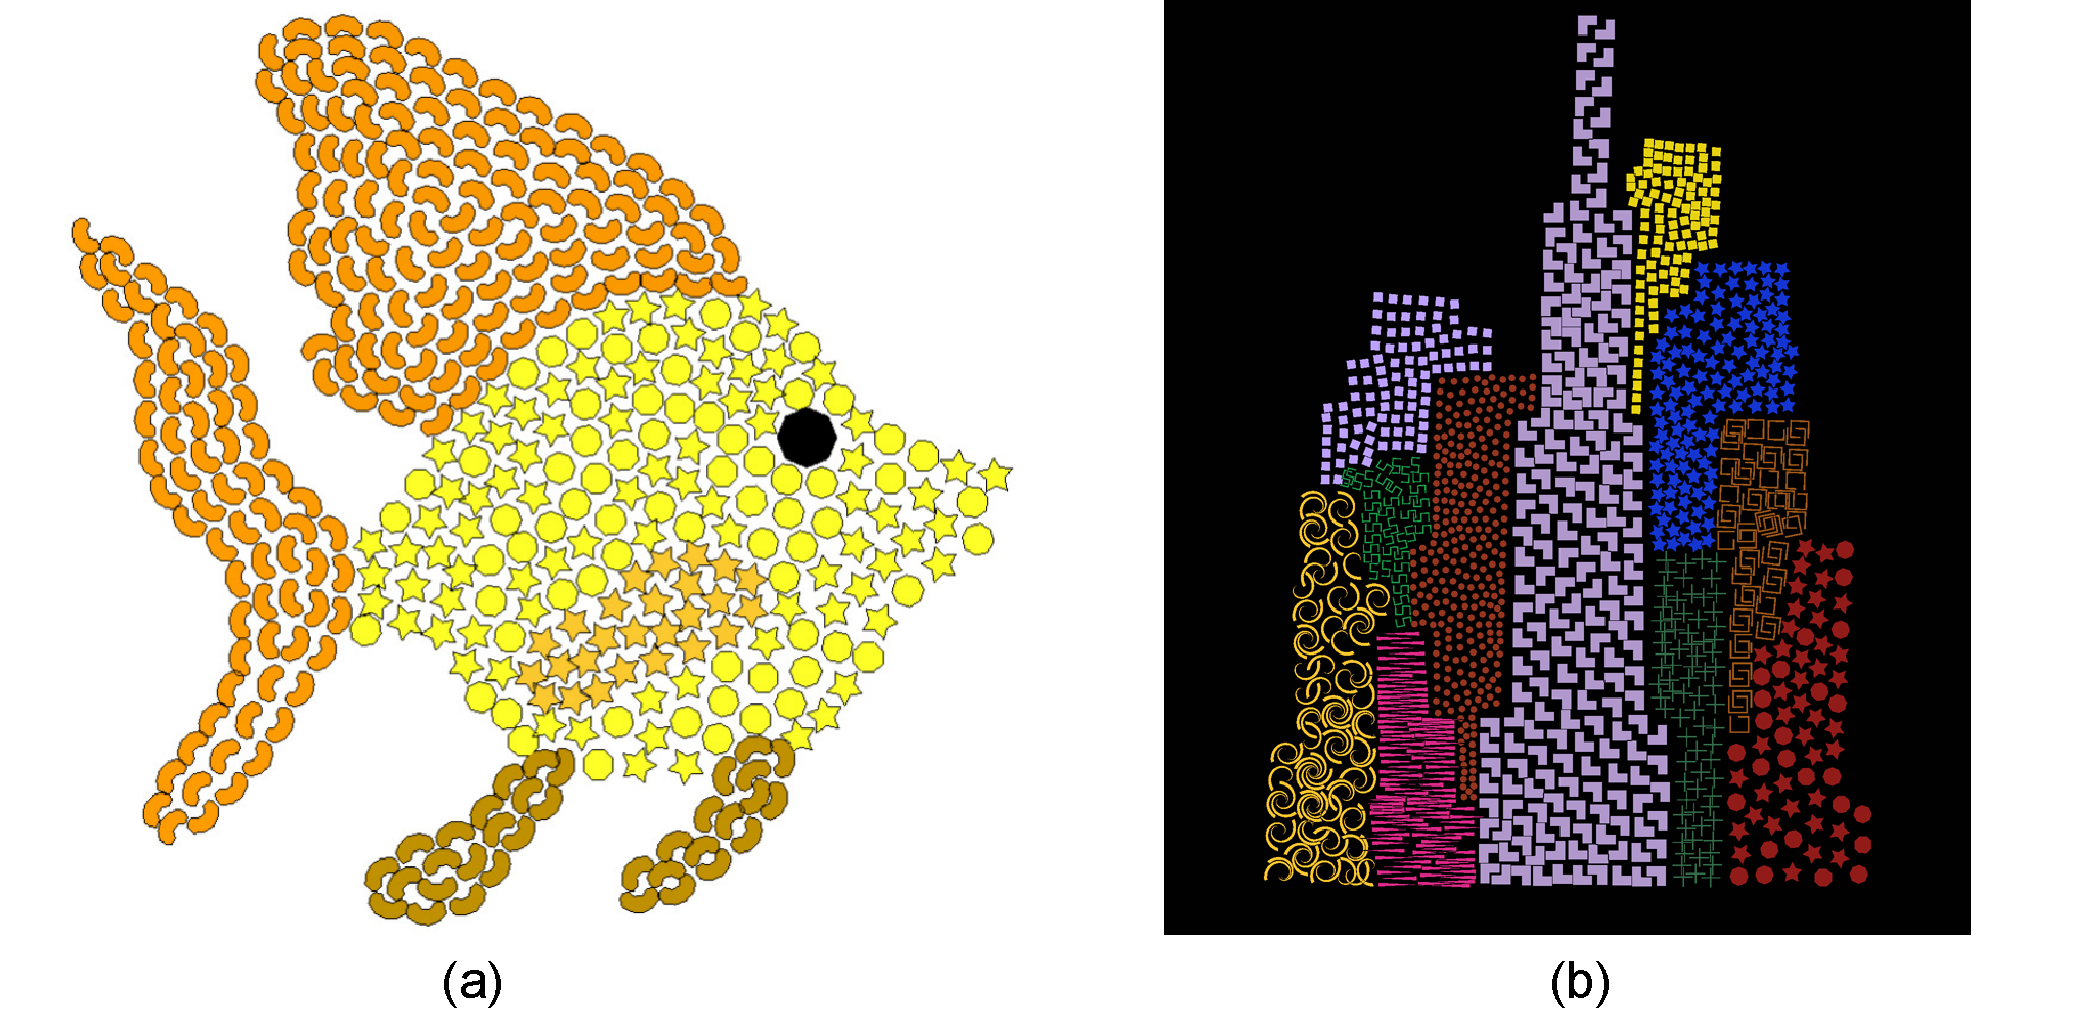
\includegraphics[width=1.0\textwidth]{figures/related/smith_dalal.pdf} 
\caption[Mosaics generated using generalized Lloyd's methods]
{\label{fig_related_secord_hausner} 
\newtext
{
Mosaics generated with generalized Voronoi diagrams.
(a) Animosaics~\cite{Smith2005}.
(b) A Spectral Approach~\cite{Dalal2006}.
}
}
\end{figure}

\newtext{As an alternative to Lloyd's method, an interactive user interface can also be used to generate mosaics.
Abdrashitov et al.~\cite{Abdrashitov2014} developed
a sketch-based \nnewtext{mosaic} interface where an artist can draw curves \nnewtext{to guide the placement of square-like elements.}
After the square elements are frozen in place, 
their boundaries are sliced to eliminate overlaps. }

%%%%%%%%%%%%%%%%%%%%%%%%%%%%%%%%%%%%%%%%%%%%%%%%%%%%%%%%%%
%\section{2D Mosaics and Packings}
%%%%%%%%%%%%%%%%%%%%%%%%%%%%%%%%%%%%%%%%%%%%%%%%%%%%%%%%%%

%\nnewtext
%{
%This section discusses related methods that generate 2D mosaics or packings,
%which are about arranging 2D elements tightly in a 2D container.
%Both mosaics and packings have a similar goal of creating a composition that have even distribution while minimizing overlaps.
%A packing with an even distribution has its positive and negative space approximately uniform.
%The gaps between elements should roughly have the same width.
%Visually, traditional mosaics often use near convex elements made of stone, ceramics, or glass,
%while 2D packings are composed of elements that have more general 
%shapes that are either convex or concave.
%}

%\nnewtext{
%An approach to generate a packing is to start with an initial configuration and 
%iteratively refine it using \textit{Lloyd's method}~\cite{McCool1992}.}
%\newtext{
%Figure~\ref{fig_lloyds_method} shows an illustration of point-based Lloyd's method.
%Given $N$ point elements, 
%we first compute a \textit{Voronoi diagram} that partitions the plane into $N$ regions such that
%all points inside a Voronoi cell are closest to its associated point element.
%Lloyd's method moves every point element to the centroid of its Voronoi cell, 
%then the Voronoi diagram is recomputed.
%The process is repeated until the distribution is even,
%that means all the point elements are located at the centroids of the Voronoi cells.
%The final structure is called a \textit{centroidal Voronoi diagram} (CVD).
%}

%\newtext
%{
%A standard CVD is generated using Euclidean distance metric, but it can be replaced
%to manipulate the shapes of Voronoi cells.
%Hausner~\cite{Hausner2001} used this idea to distribute square elements into a container 
%region, simulating the appearance of traditional mosaics (Figure~\ref{fig_related_hausner}). 
%This can be achieved by using Manhattan distance metric so that Voronoi cells resemble squares instead of hexagons.
%This approach can only position the square elements to be centered at the Voronoi centroids, and it must
%incorporate a vector field to modify the orientation of the metric
%and rotate the square elements. 
%In conclusion, Hausner's approach is only suitable for square elements as
%more complicated shapes such as long rectangles would have severe overlaps.
%More recently, Javid et al.~\cite{Javid2019} constructed a metric that 
%incorporates a spatial distance, a color distance, and an elongation factor. Their resulting
%Voronoi cells have elongated shapes, resembling pebble-like mosaics.}

\section{2D Packings}

\newtext{
This section discusses packings composed of elements that resemble 
man-made objects, geometry, letterforms, plants, or animals.
Unlike decorative mosaics, 
packings are mostly found in logo design and graphic design.
Some packing styles are reminiscent \nnewtext{to paintings by Giuseppe Arcimboldo, 
like the one} shown in Figure ~\ref{fig_related_arcimboldo}.
Most packing methods drift away from Lloyd's method in favor of data-driven methods (Figure~\ref{fig_taxonomy_method}b) and 
deformation-driven methods (Figure~\ref{fig_taxonomy_method}c).}

%\nnewtext
%{
%This section discusses packing methods that fall into the categories of data-driven (Figure~\ref{fig_taxonomy_method}b) and 
%deformation-driven (Figure~\ref{fig_taxonomy_method}c).
%Unlike mosaics, these packings are composed of 
%more intricate elements that resemble man-made objects, letterforms, plants, or animals.
%Additionally, some packing styles are reminiscent to one of Giuseppe Arcimboldo's paintings 
%shown in Figure ~\ref{fig_related_arcimboldo}).
%}

\newtext{A data-driven method requires an input element library to find compatible elements (Figure~\ref{fig_related_jim_pad}).}
\newtext{\nnewtext{Typically, elements are placed} one by one until the container area is filled.
A shape matching algorithm selects an 
element from the library that has the best compatibility with the previously placed elements or the container boundary.
Jigsaw Image Mosaics~\cite{Kim2002} uses a geometric hashing technique to find
compatible elements. \nnewtext{JIM} places elements using a greedy approach, but is able to backtrack 
if a previous configuration is more optimal.
Pyramid of Arclength Descriptor (PAD)~\cite{Kwan2016} is a curvature-based shape descriptor that
can find new elements that partially match
existing element boundaries as a container \nnewtext{is} being filled. }


\newtext{\newtext{An alternative approach to data-driven methods} is to initially partition a container into smaller segments
\nnewtext{and} independently replace each segment with a matching element \nnewtext{taken from the library}.
This is desirable if the container has colours or salient parts that need to be emphasized.
Huang et al.~\cite{Huang2011} proposed a data-driven approach that generates Arcimboldo-like collages
by arranging cutout images collected from the internet.
Their container is a larger cutout image which is partitioned into parts
using an image segmentation algorithm.
Each part is then replaced with a smaller cutout image that has a similar shape and colour.
}

\newtext
{
All these data-driven methods require a large element library.
The more elements in the library, the better the chances of finding compatible elements.}
\newtext
{
For example, \nnewtext{JIM} required about 900 elements, PAD used a library with more than 120 elements 
(see Figure~\ref{fig_taxonomy_method}), 
and Huang et al.\ needed about 5000 elements.}
\newtext
{However, a bigger database means increased \nnewtext{computation time} and
collecting a large number of elements is not always feasible.}


%Techniques like JIM and PAD pack elements without deforming them. 
%But element shapes never have perfectly compatible boundaries, and the packing process allows some overlaps to arise between neighbouring elements. 
%These techniques optionally post-process elements by locally deforming their boundaries to suppress overlaps.  
%While these local adjustments improve compatibility, 
%they cannot interact with the placement process, and 
%a large element library is still required to generate satisfactory 

\nnewtext{ 
The placement process in JIM and PAD is being done without shape deformation.
As shown in their results in Figure~\ref{fig_related_jim_pad}, 
element shapes never have perfectly compatible boundaries, and 
the packing process allows some overlaps to arise between neighbouring elements. 
These techniques optionally post-process elements by locally deforming their boundaries to suppress overlaps.  
While these local adjustments improve compatibility, 
they cannot influence the placement process, and 
a large element library is still required to generate satisfactory packings.
}

%\nnewtext{ 
%After the container is filled, these data-driven methods permit some elements to overlaps,
%which are later corrected using deformation.
%This is a post-processing step where the elements are frozen in place and
%the deformation is applied locally near element boundaries.
%The deformation improves element compatibilities, 
%but only locally as these methods still need a large element library to generate satisfactory packings.} 

\begin{figure}
\centering
\includegraphics[width=1.0\textwidth]{figures/related/arcimboldo.pdf} 
\caption[Vertumnus painting by Giuseppe Arcimboldo]
{\label{fig_related_arcimboldo} 
\newtext
{
\nnewtext{\textit{Vertumnus} (ca. 1590), by Giuseppe Arcimbolo, which illustrates}
a packing of plants, vegetables, and fruits
(Skokloster Castle, Skokloster, Sweden). 
}
}
\end{figure}

\begin{figure}
\centering
\includegraphics[width=1.0\textwidth]{figures/related/jim_pad.pdf} 
\caption[Packings generated by JIM and PAD]
{\label{fig_related_jim_pad} 
\newtext
{
Data-driven methods:
(a) Jigsaw Image Mosaics~\cite{Kim2002}.
(b) Pyramid of Arclength Descriptor~\cite{Kwan2016}. 
}
}
\end{figure}




\begin{figure}
\centering
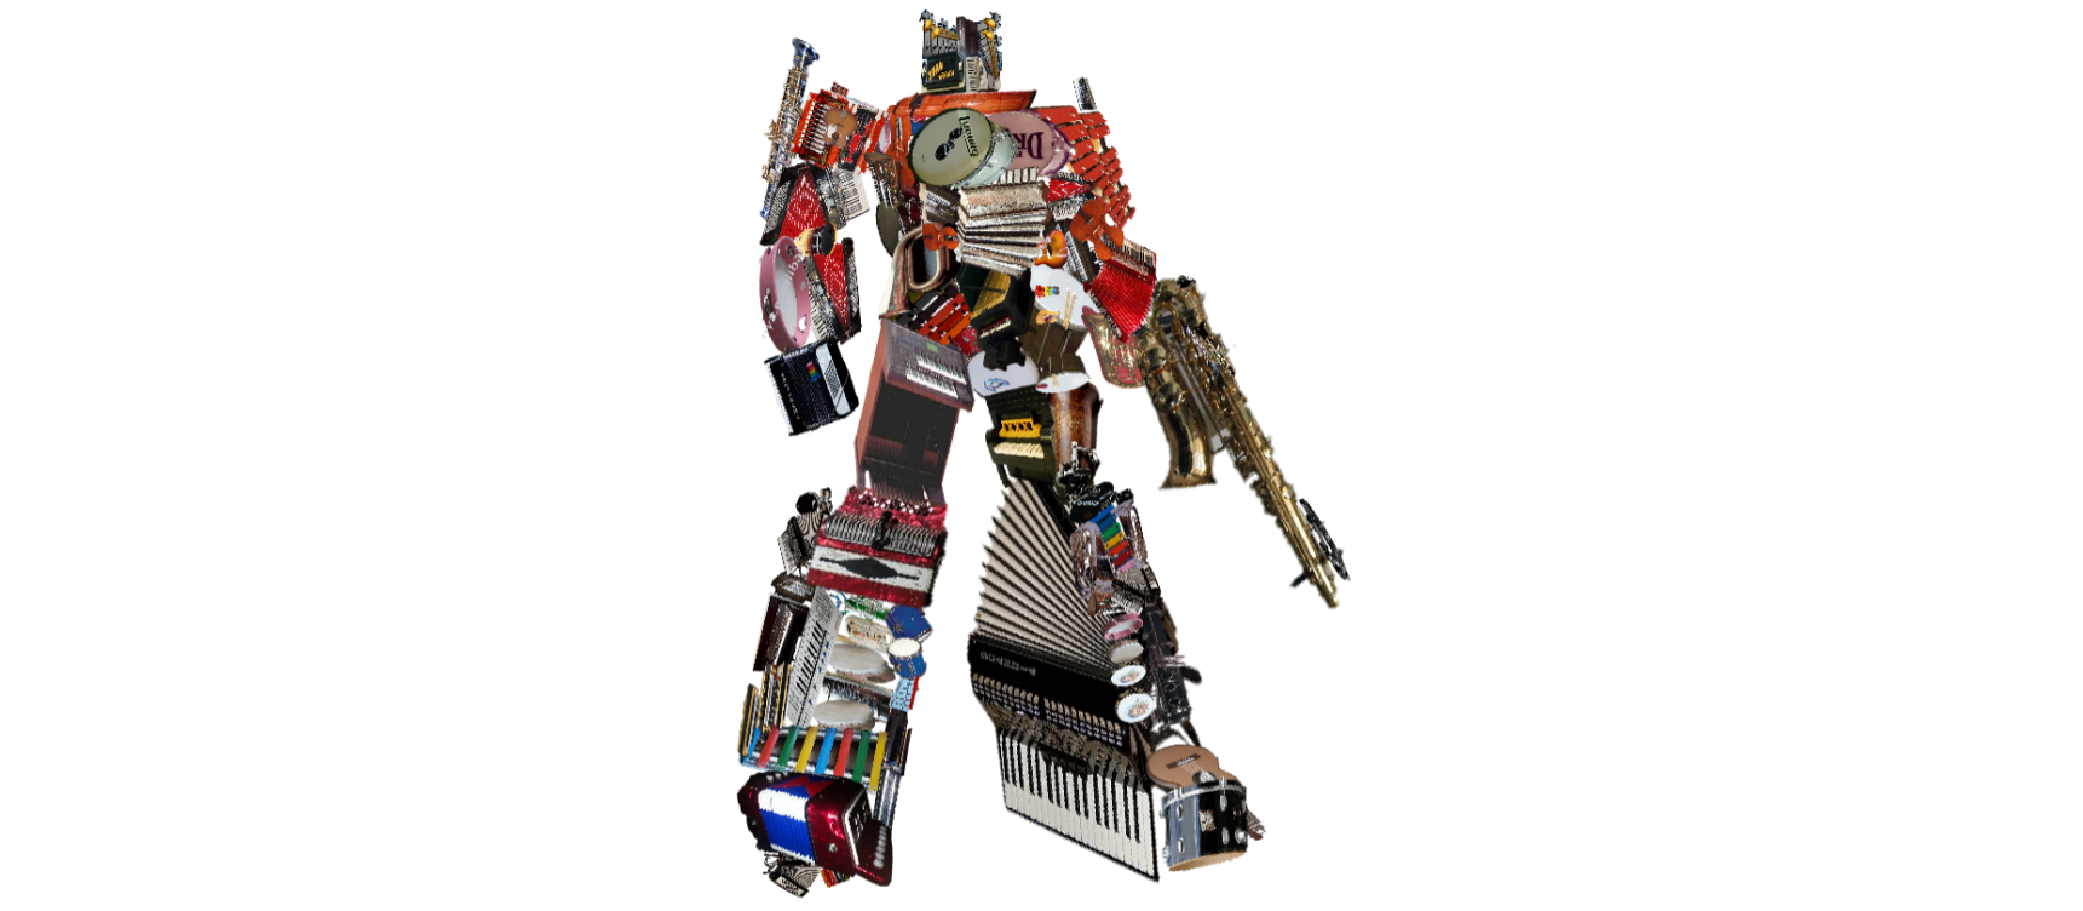
\includegraphics[width=1.0\textwidth]{figures/related/optimus.pdf} 
\caption[An Arcimboldo-inspired 2D packing]
{\label{fig_related_optimus} 
\newtext
{
An Arcimboldo-inspired 2D packing of overlapping elements~\cite{Huang2011} .
}
}
\end{figure}

\newtext
{
Instead of allowing shape compatibilities to arise organically in a large collection of elements, 
we can deform elements to manufacture those compatibilities.
A deformation-driven method can create packings based on much smaller element libraries.
Xu and Kaplan~\cite{Xu2007} and Zou et al.~\cite{Zou2016} constructed calligraphic packings by filling a container with a small
number of letter elements composing one or two words (Figure~\ref{fig_taxonomy_method}c and ~\ref{fig_calligraphy_packing}a). 
Xu and Kaplan's method is able to fill the container but 
\nnewtext{the arrangement and deformation of the letters can make the calligram difficult to read}.
The improved method by Zou et al. can achieve better readability by computing
the medial axis of the container where letter elements are anchored.
However, these calligraphic packing methods require significant deformation 
so they are not able to preserve the \nnewtext{characters of the original letterforms}.
\nnewtext{In other work}, 
Peng et al.~\cite{Peng2014} proposed a method that packs and deforms
simple polygon and polyomino elements to generate layouts for urban planning or indoor space, 
although their method cannot handle more complicated element shapes. 
An example of a generated indoor layout is \nnewtext{shown} in Figure~\ref{fig_office}.
}


\newtext
{
These data-driven methods and deformation driven methods inspire \nnewtext{us} to develop new packing methods.
%We see an opportunity to develop better packing methods that combine 
%the best of both worlds of data-driven methods and deformation driven methods.
In JIMs and PAD packings, deformation is a \nnewtext{post-processing operation used for local touch-ups}.
In \nnewtext{calligraphic} packings and polyomino layouts, the deformation methods are limited to specific element shapes.
We would like to use deformation as the core of the packing process and generate \nnewtext{packings}
with more general styles similar to JIMs and PAD packings.
}

%\nnewtext
%{
%Unfortunately,
%these data-driven methods are limited to specific designs: calligraphies of letterforms and urban layouts of rectangular shapes.
%We see an opportunity to use deformation-driven approach to generate packings with more general styles composed
%of nature or everyday objects similar to JIMs and PAD packings.
%}


%\nnewtext
%{
%}

\begin{figure}
\centering

\includegraphics[width=1.0\textwidth]{figures/related/calligraphy.pdf} 
\caption[A calligraphy packing of an ``elephant'']
{\label{fig_calligraphy_packing} 
\newtext
{
A deformation-driven packing of a calligraphic ``elephant''~\cite{Xu2007}.
}
}
\vspace{20pt}
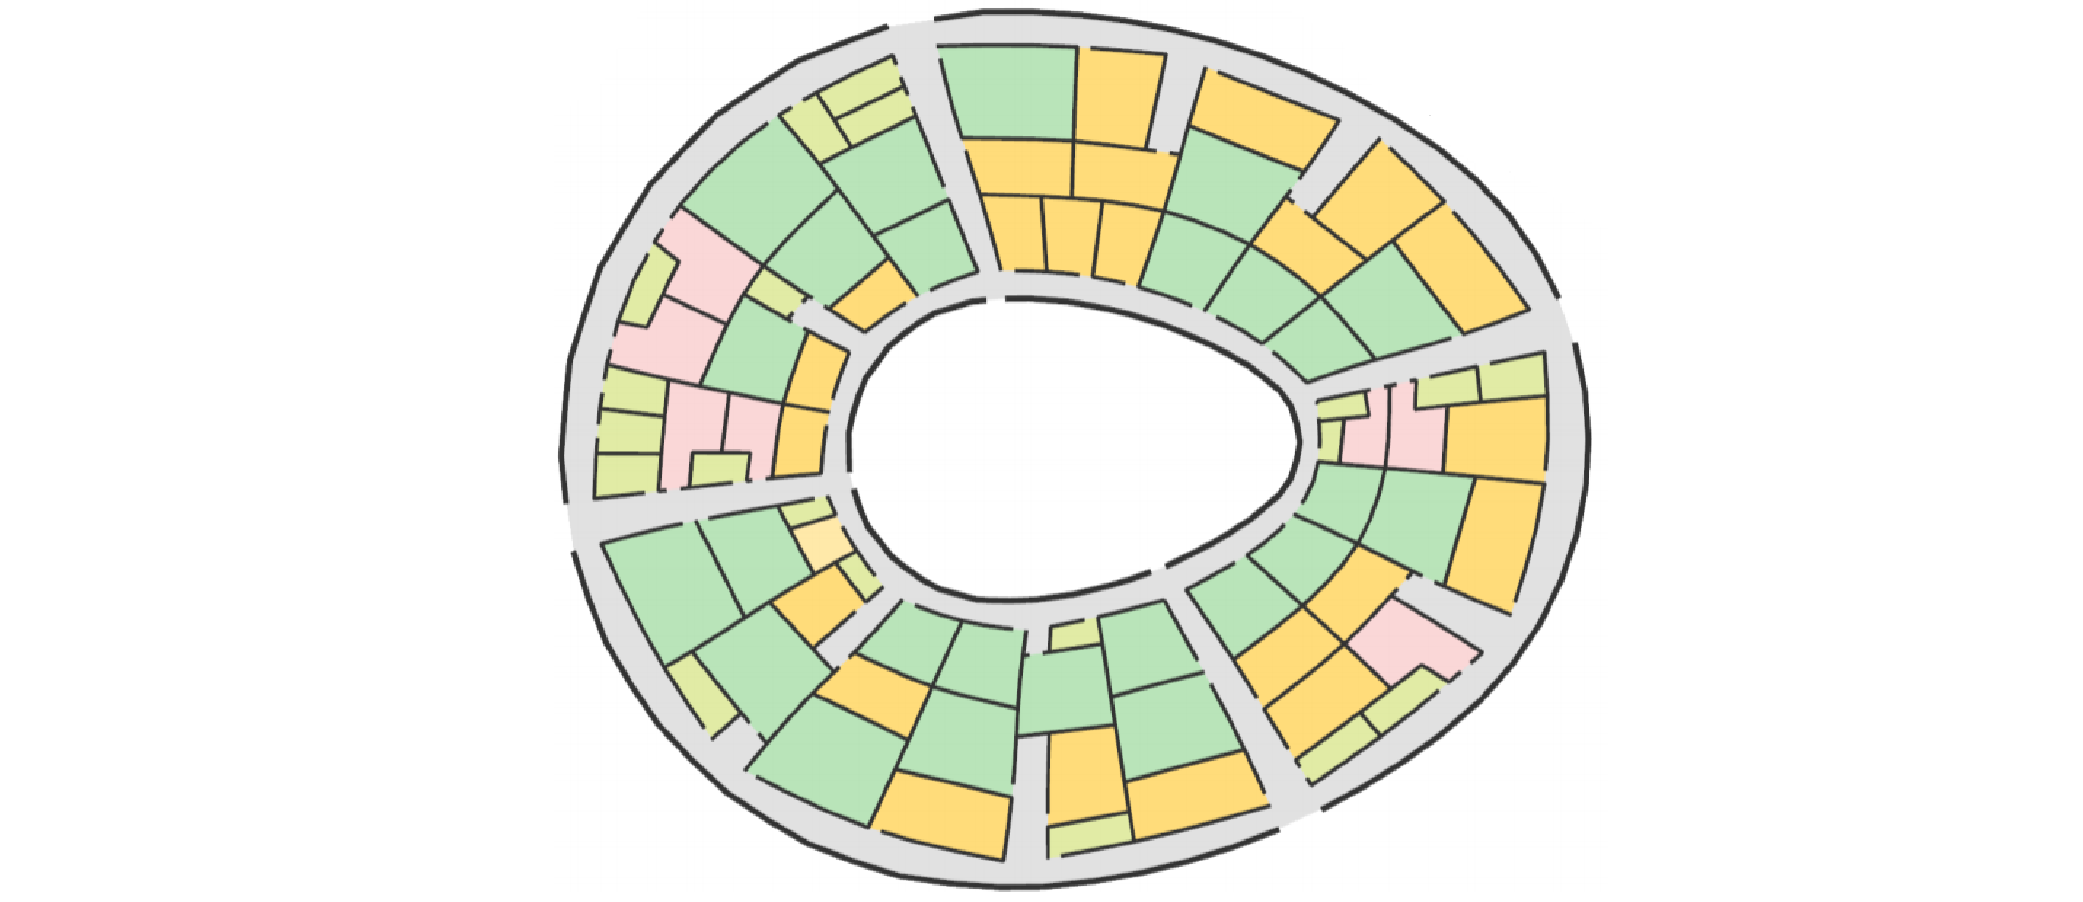
\includegraphics[width=1.0\textwidth]{figures/related/layout.pdf} 
\caption[An office layout generated by packing \newline deformable rectangle and polyomino elements]
{\label{fig_office}
\newtext
{
An office layout generated by packing deformable rectangle and polyomino elements~\cite{Peng2014}.
}
}
\end{figure}




%%%%%%%%%%%%%%%%%%%%%%%%%%%%%%%%%%%%%%%%%%%%%%%%%%%%%%%%%%
\section{Tilings}
\label{related_wrok_tiling}
%%%%%%%%%%%%%%%%%%%%%%%%%%%%%%%%%%%%%%%%%%%%%%%%%%%%%%%%%%

\newtext
{
As elements reach perfect compatibility, a packing turns to a tiling, \nnewtext{such as the example} in Figure~\ref{fig_related_escherization}a.
The element boundaries interlock, leaving no negative space.
\nnewtext{Kaplan and Salesin introduced Escherization~\cite{Kaplan2000, Kaplan2004},
a technique that deforms} one or two 
input elements into shapes that can tile the plane.
The tiles always fill the entire plane, and are not intended for filling a bounded container.}
\newtext{Given an input \nnewtext{element $S$}, they performed a search in a parameterized tiling space to find its
deformed variant $T$.
Due to deformation,}
\newtext{$T$ is often perceptually unrecognizable from its silhouette unless an interior picture is added.}
\newtext{
Kaplan and Salesin's method has a better chance to find $T$ if \nnewtext{$S$} has shallow concavities.
More recent methods~\cite{Koizumi2011, Nagata2020} are able to solve the Escherization problem more efficiently and can deal with shapes 
that have deeper concavities.}


%Given an input element $E$ they look for a similar tileable element $T$
%in a parameterized tiling space using simulated annealing.
%The original heuristic method has a better chance to find $T$ if $E$ has less concavity, but more recent methods
%are able to tile shapes 
%The original heuristic method can only deal withfail to find $T$ if $E$ has deep concavity, for example, a ``G'' shape.
%However, more recent methods are able to deal with this issue.

\newtext
{
Past research has proposed methods
to replicate the figure-ground reversal style of Escher's 
\nnewtext{\textit{Sky and Water}},
in which elements serve as both positive and negative space depending 
on the viewer's perception~\cite{Kaplan2004, Sugihara2009, Lin2018}.
\nnewtext{Two input elements $S_1$ and $S_2$ are placed at opposite ends of a canvas.
They are then copied, arranged, and deformed until they meet in a tiling in the middle, with copies of each shape acting as the other's negative space
(Figure~\ref{fig_related_escherization}b).
The gradual evolution of tile shapes can also be found in Escher-like metamorphoses and Parquet Deformations. 
As shown in Figure~\ref{fig_related_escherization}c, tilings that can be interpreted as a kind of spatial animation.}
Kaplan~\cite{Kaplan2010} proposed several element evolution schemes to generate \nnewtext{metamorphoses}:
a grid-based curve evolution, iterated function systems, and organic labyrinth simulations.
}

\begin{figure}
\centering
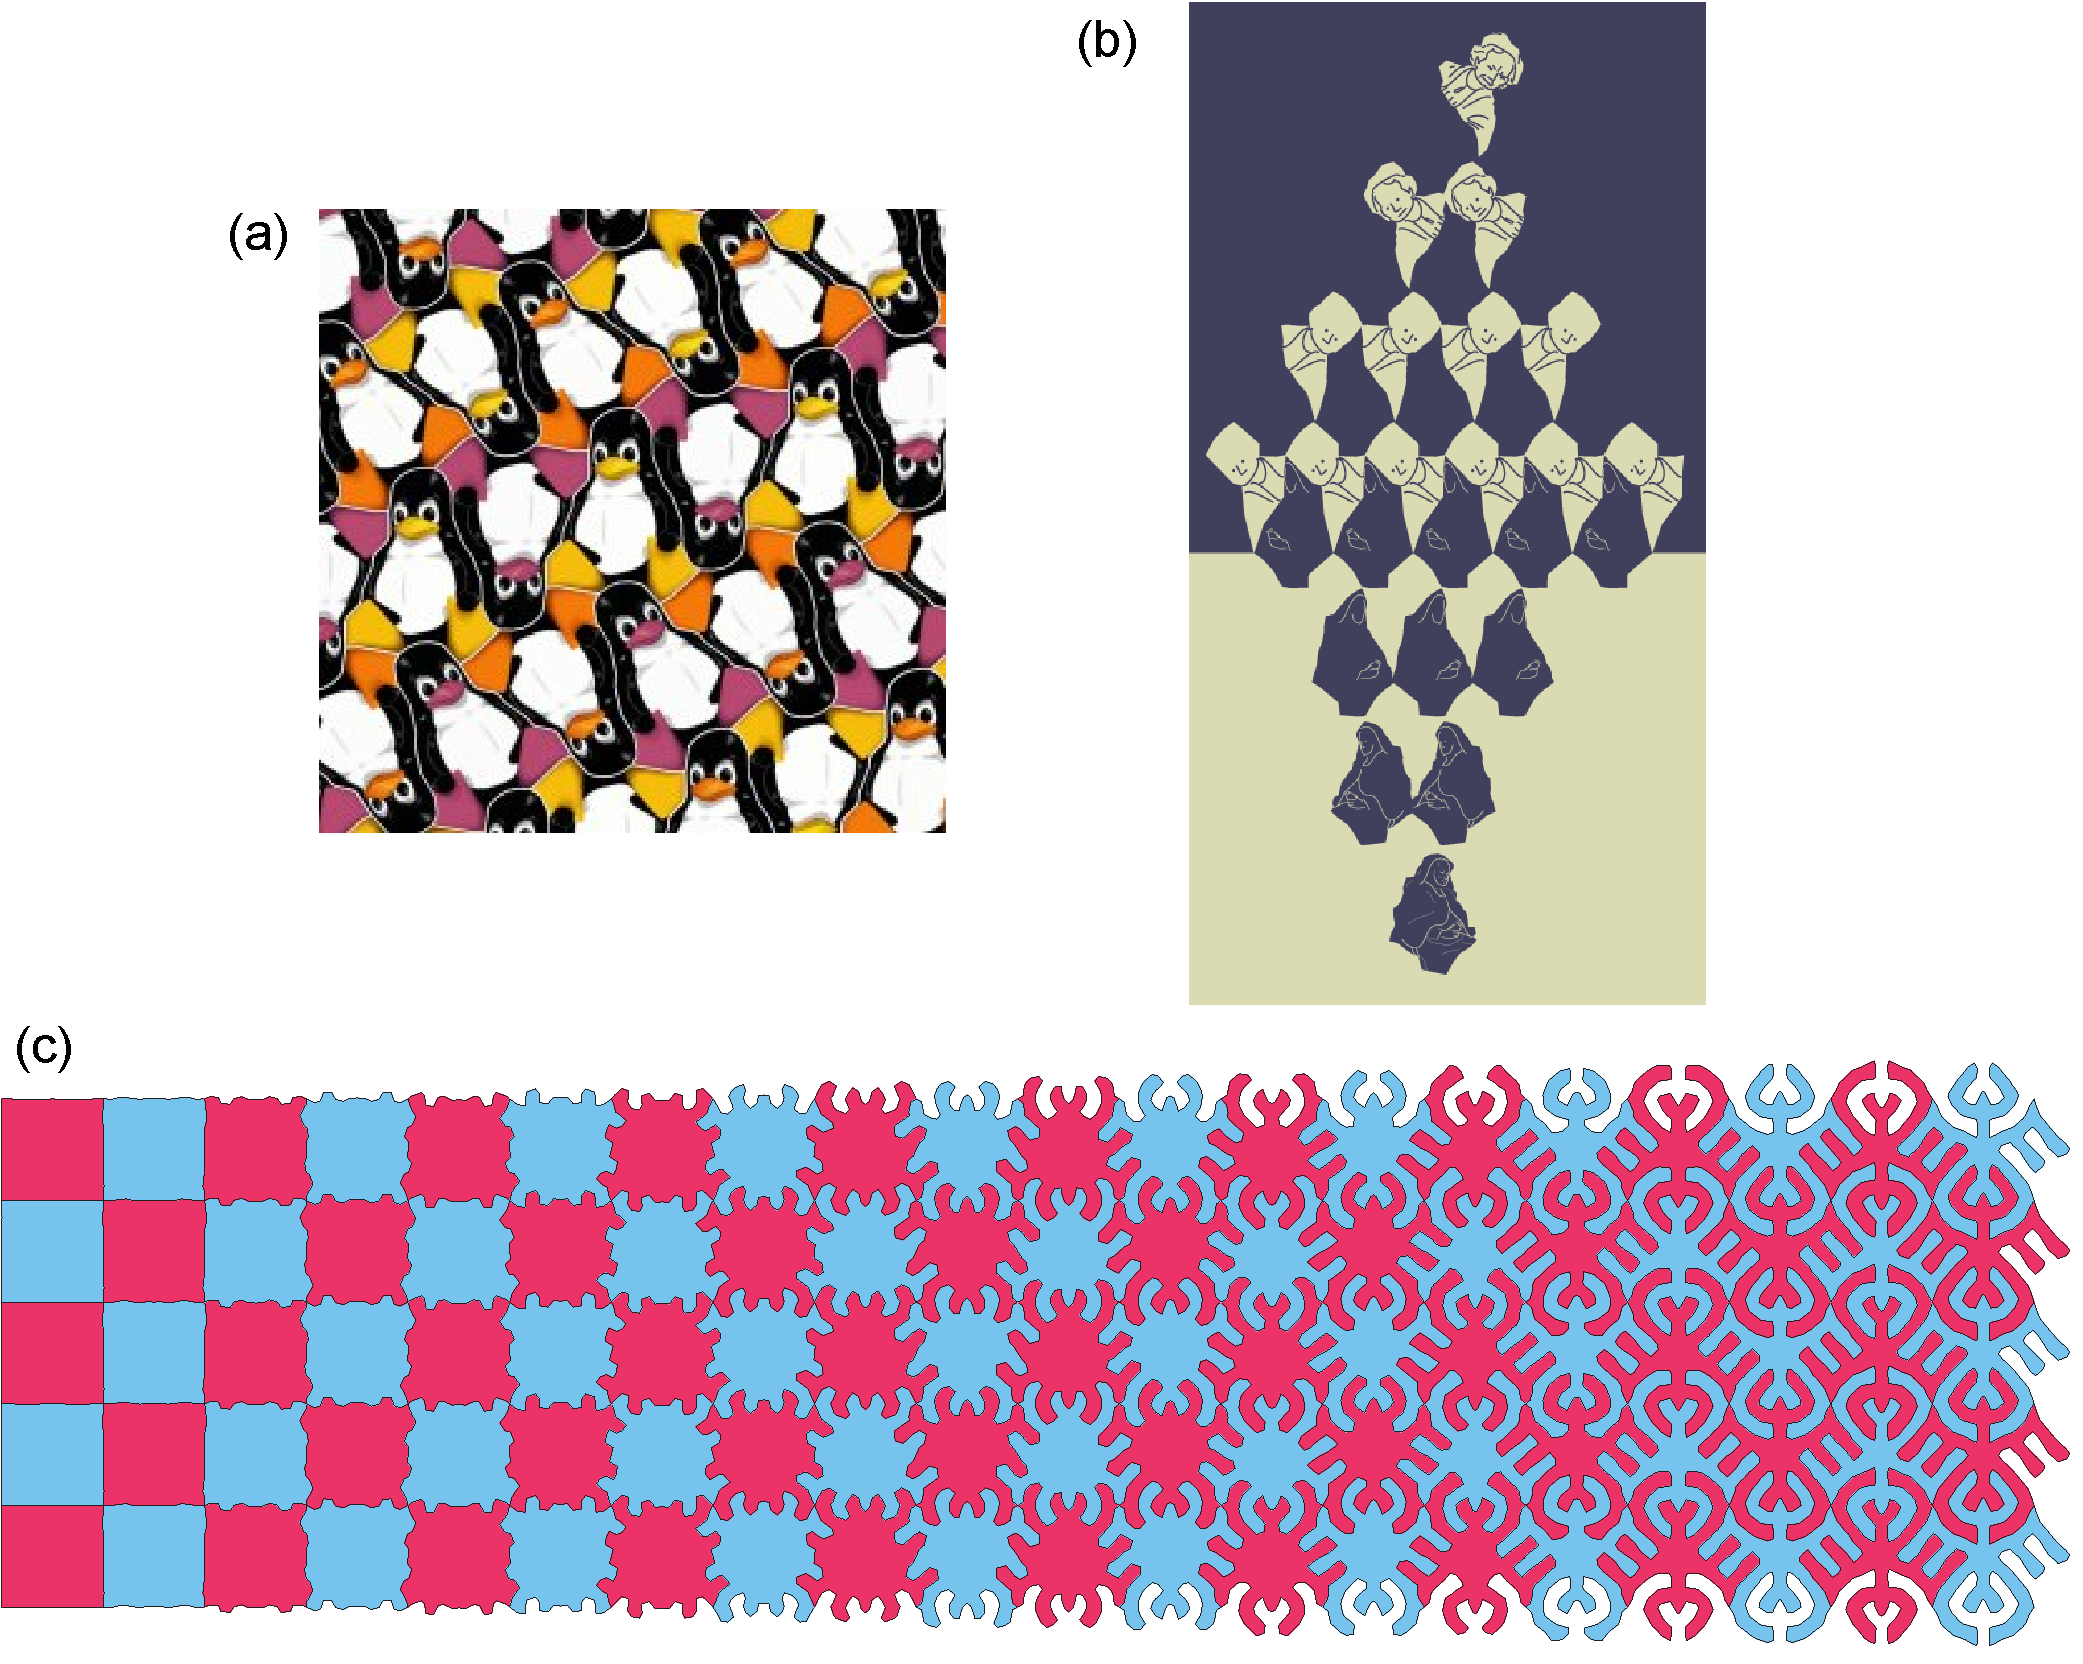
\includegraphics[width=1.0\textwidth]{figures/related/tilings.pdf} 
\caption[Tilings]
{\label{fig_related_escherization} 
\nnewtext
{
(a) A tiling of tux penguins~\cite{Kaplan2000}.
(b) Sky and water tiling style~\cite{Kaplan2004}. \\
(c) Metamorphosis tiling style~\cite{Kaplan2010}.
}
}
\end{figure}

%Given two elements $S_1$ and $S_2$, each is placed on the opposite side of a rectangular canvas.
%They are then copied, arranged, and deformed to interlock each other.
%The farther a copy from the original element, the more deformed it is and the


%\newtext
%{
%Lin et al.~\cite{Lin2018} generated ground-reversal compositions that resemble Escher's Sky and Water I,
%where elements serve as both positive and negative space depending on the viewer's perception.
%Given two elements $S_1$ and $S_2$, each is placed on the opposite side of a rectangular canvas.
%They are then copied, arranged, and deformed to interlock each other.
%The farther a copy from the original element, the more deformed it is, 
%creating a ``fading effect'', $S_1$ and $S_2$ spatially fade to nothingness.
%This work is data-driven, the user needs to provide $S_1$, 
%and the method tries to find a compatible element $S_2$ from a library.
%}





%%%%%%%%%%%%%%%%%%%%%%%%%%%%%%%%%%%%%%%%%%%%%%%%%%%%%%%%%%
\section{Discrete Texture Synthesis}
%%%%%%%%%%%%%%%%%%%%%%%%%%%%%%%%%%%%%%%%%%%%%%%%%%%%%%%%%%



\newtext
{
Some past work has sought to adapt example-based texture synthesis methods
from raster images to vector graphics, producing distributions of
rigidly transformed elements that mimic the statistics of an \textit{exemplar}, 
an example can be seen in Figure~\ref{fig_discrete_texture}.}
\nnewtext{For raster-based texture synthesis methods, readers can refer to a survey paper
compiled by Wei et al.~\cite{Wei2009}.}
\newtext{These techniques are all concerned with replicating
the distribution of positive space in the exemplar, and less about negative space.}
\newtext{An element is represented as a single point, which is adequate for small near-convex elements.
Barla et al.~\cite{Barla2006} and Ijiri et al.~\cite{Ijiri2008} used a growth model that copies small neighbourhoods
from the exemplar into a larger output texture.  
Hurtut et al.~\cite{Hurtut2009} developed a statistical sampling method based
on multitype point processes.  
AlMeraj et al.~\cite{AlMeraj2013}
stamped out copies of the exemplar and discarded overlapping elements.
Loi et al.~\cite{Loi2017} developed a texture synthesis method that
can specify global arrangements, local arrangements, or a blend of multiple arrangements.
}

\newtext
{
For larger concave elements, a single point representation is not enough.
Ma et al. ~\cite{Ma2011} used a sample-based representation that
is created by generating a sparse set of points inside an element.
They later distributed these points using a neighbourhood metric and an iterative optimization.
Unlike previous work, they were able synthesize textures with long deformable elements, for example, spaghetti.
Ma et al. later extended their work to accept animated elements~\cite{Ma2013}, where
each sample point has a spatial and time position, turning the problem to spacetime texture synthesis.
More recently, Hsu et al.~\cite{Hsu2020} adapted the sample-based representation into an interactive tool
where an artist can initially distribute elements by drawing strokes
which are then optimized using a Lloyd-like optimization.
}
%Most discrete texture synthesis method treat a single element
%Ma et al.~\cite{Ma2011} used sample-based element representation 
%Ma et al.~\cite{Ma2011} use sparse point samples to represent an element, which
%give an advantage of distributing 


\begin{figure}
\centering
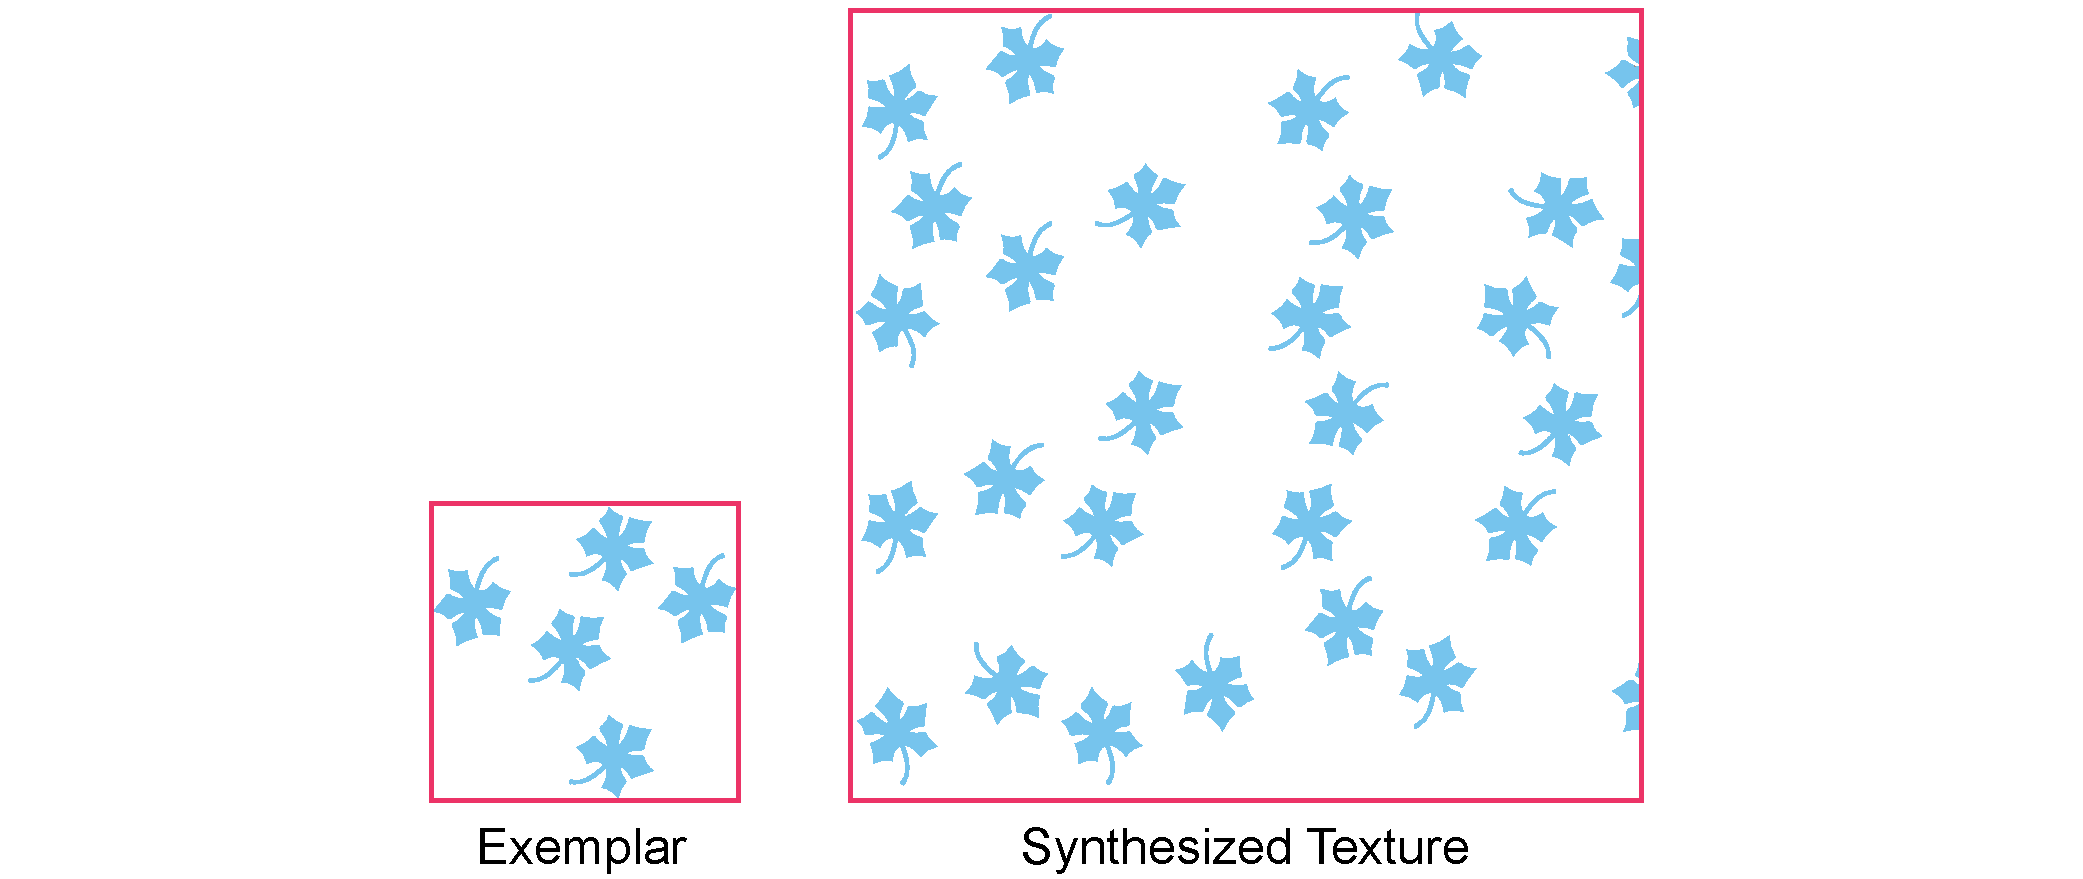
\includegraphics[width=1.0\textwidth]{figures/related/discrete_texture.pdf} 
\caption[A discrete texture]
{\label{fig_discrete_texture} 
\newtext
{
An example of discrete texture synthesis~\cite{AlMeraj2013}.
}
}
\end{figure}



%%%%%%%%%%%%%%%%%%%%%%%%%%%%%%%%%%%%%%%%%%%%%%%%%%%%%%%%%%
\section{3D Packings}
%%%%%%%%%%%%%%%%%%%%%%%%%%%%%%%%%%%%%%%%%%%%%%%%%%%%%%%%%%
\newtext{Collages are arrangements of overlapping elements, similar to
portrait paintings by Giuseppe Arcimboldo.
Gal et al.~\cite{Gal2007B} presented a method for constructing 3D
collages \newtext{(Figure~\ref{fig_related_gal_ma_chen}a)}.  
They filled a 3D container with overlapping 3D elements using a greedy
approach and a partial shape matching algorithm.}
\nnewtext{This work can be seen as a JIM-like technique in 3D, except that there is more tolerance for overlaps.}
\newtext{
Similar to the work of Gal et al., Theobalt et al.~\cite{Theobalt2007}
developed a method to generate animated 3D collages, which we will discuss more in Chapter~\ref{chapter_animationpak}.}
\newtext{\nnewtext{In other work}, Huang et al.~\cite{Huang2014} designed a method
to generate mechanical collages, such as giant robots.
All these collage methods require a 3D shape database.} %so they are considered as data-driven. 
%Both these collage methods require a 3D shape database so they can be considered as data-driven. 


\newtext
{
The cutting and packing problem (C\&P) is defined as cutting a large object into smaller parts 
which are then packed inside a container.
C\&P is popular in manufacturing and 3D printing because
objects can be produced with less waste material and packed into a smaller box.
A good cutting process is critical in C\&P: if it can decompose the input object
into simpler parts, then the packing process can be easier.
Chernov et al.~\cite{Chernov2010} proposed a method to decompose a large object
into smaller ``phi objects'' that can be packed more efficiently.
A phi object is defined as a shape whose surface boundaries 
are flat, spherical, cylindrical, or conical.
Vanek et al.~\cite{Vanek2014} introduced PackMerger,
a method to pack thin shells which can be assembled together into
a larger watertight object.
In follow up work, Chen et al.~\cite{Chen2015} introduced Dapper,
a method to cut and pack volumetric printed objects.
}

\newtext
{
In engineering, packings are useful for a number of applications, 
such as product packaging, circuit designs, or mechanical layouts.
This requires elements to be packed without any overlap.
Cagan et al.~\cite{Cagan2002} compiled a survey of 3D packing approaches such as
gradient methods, simulated annealing, and genetic algorithms.
Byholm et al.~\cite{Byholm2009} developed a method
to pack voxelized elements, which are computationally easier for collision detection.
Ma et al.~\cite{Ma2018} proposed a heuristic method to pack non-overlapping triangular meshes 
\nnewtext{(Figure~\ref{fig_related_gal_ma_chen}b)}.
}



%%%%%%%%%%%%%%%%%%%%%%%%%%%%%%%%%%%%%%%%%%%%%%%%%%%%%%%%%%
\section{Packings on Surfaces}
%%%%%%%%%%%%%%%%%%%%%%%%%%%%%%%%%%%%%%%%%%%%%%%%%%%%%%%%%%

Some recent work has explored the elaboration of ornamental
patterns on surfaces, under constraints imposed by fabrication, such as connectivity.  
\nnewtext{Schiftner et al.~\cite{Schiftner2009} introduced Circle Packing meshes,
a special kind of triangle mesh,
where the incircles of two neighbouring triangles have the same contact point on the shared edge,
forming a packing of circles or spheres.}
Chen et al.~\cite{Chen2016} developed a method to generate a filigree pattern,
which is an arrangement of decorative thin rod elements on a surface.
Given an initial random configuration of overlapping elements, their method
removes overlaps by either deforming or trimming the rods.
In similar work, Zehnder et al.~\cite{Zehnder2016} 
proposed a semi-automated tool for deforming ornamental curves to cover a surface, \nnewtext{as} shown in 
Figure~\ref{fig_related_gal_ma_chen}c. 
They \nnewtext{start} with an \nnewtext{initial, overlap free} configuration of scaled down elements. 
They \nnewtext{then grow} the elements, \nnewtext{avoiding} overlaps using curve deformation.
Chen et al.~\cite{Chen2017} generated modular surfaces by
computing contact point networks of rigid elements, \nnewtext{as shown} in Figure~\ref{fig_related_gal_ma_chen}d.
Bian et al.~\cite{Bian2018} used Wang tiles made of element parts to generate filigree patterns.
Mart\'{\i}nez et al.~\cite{Martinez2019} developed \nnewtext{a variant of Lloyd's method} to generate
star-shaped tiling patterns that are printed onto tracery sheets.
Their method works by constructing a star-shaped metric to manipulate the Voronoi cell shapes. 

%\begin{figure}
%\centering
%\includegraphics[width=1.0\textwidth]{figures/related/arcimboldo_gal.pdf} 
%\caption[Examples of 3D packing arrangements]
%{\label{fig_related_arcimboldo_gal} 
%\newtext
%{
%3D packing arrangements:
%(Left) Vertumnus painting by Giuseppe Arcimboldo (Skokloster Castle, Skokloster, Sweden). 
%(Right) An Arcimboldo-like 3D packing~\cite{Gal2007B}.
%}
%}
%\end{figure}

%\makeatletter % brooo
%\setlength{\@fptop}{0pt} % brooo
%\makeatother % brooo
%\begin{figure}
%\centering
%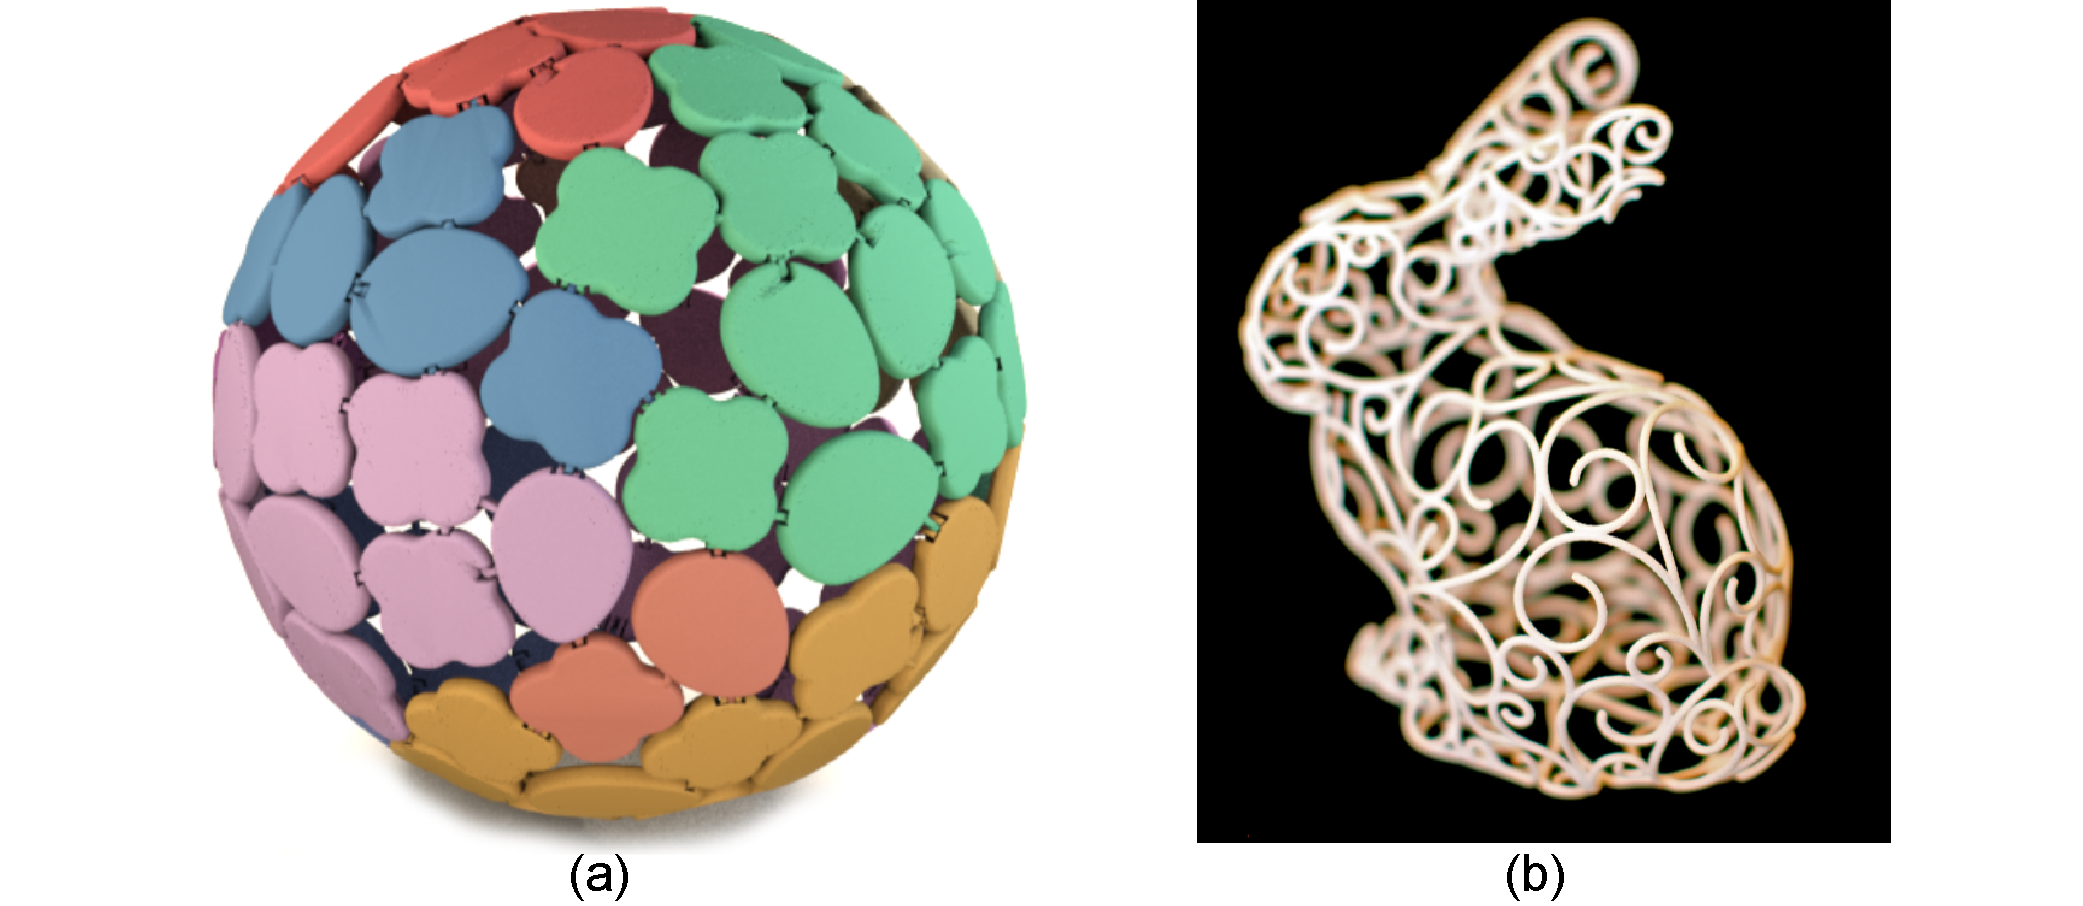
\includegraphics[width=1.0\textwidth]{figures/related/chen_zehnder.pdf} 
%\caption[Two example of packings on surfaces]
%{\label{fig_related_chen_zehnder} 
%\nnewtext
%{
%Two example of packings on surfaces:
%(a) Elements packed on a surface and connected by hinges~\cite{Chen2017}.
%(b) Curve elements arranged on a bunny surface~\cite{Zehnder2016}.
%}
%}
%\end{figure}

%\makeatletter % brooo
%\setlength{\@fptop}{0pt} % brooo
%\makeatother % brooo
\begin{figure}
\centering
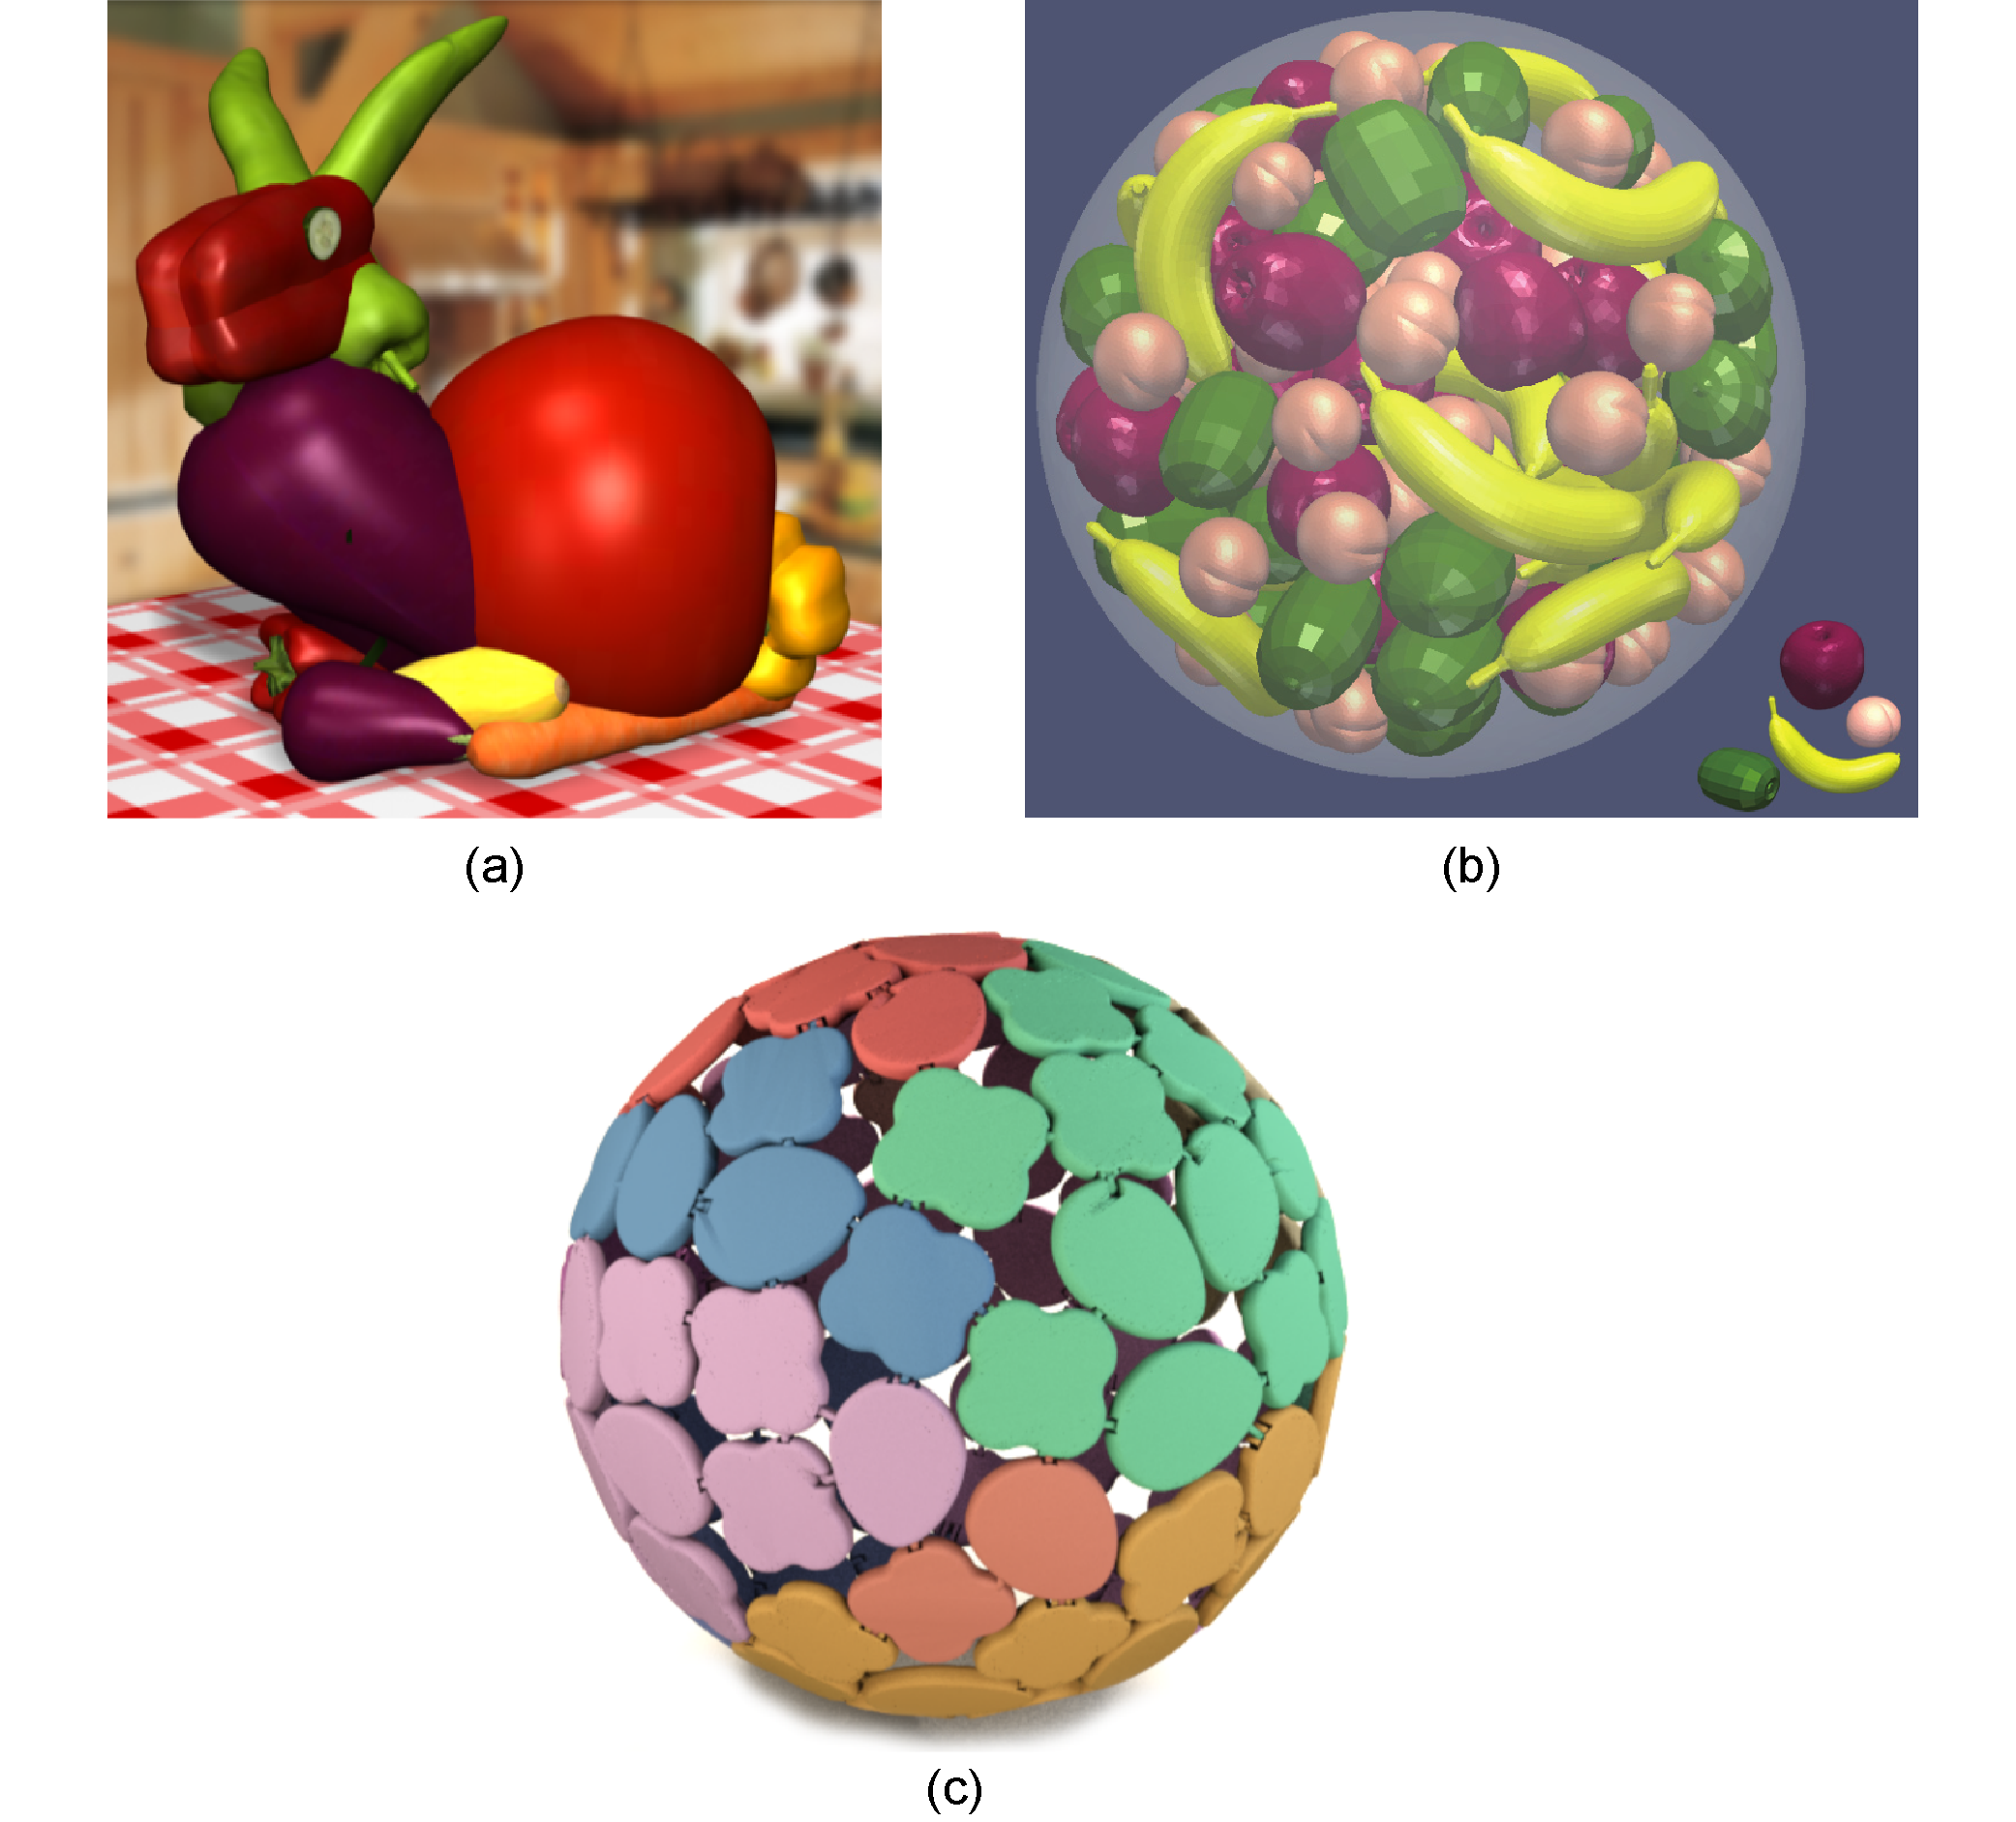
\includegraphics[width=1.0\textwidth]{figures/related/gal_ma_chen.pdf} 
\caption[Examples of 3D packings and packings on surfaces]
{\label{fig_related_gal_ma_chen} 
\newtext
{
Examples of 3D packings and packings on surfaces.
(a) An Arcimboldo-like packing of overlapping 3D elements~\cite{Gal2007B}. 
(c) A packing of non-overlapping 3D elements~\cite{Ma2018}.
(c) Deformed curve elements that fill a surface~\cite{Zehnder2016}.
(d) \nnewtext{A surface packed with elements connected to each other by hinges}~\cite{Chen2017}.
}
}
\end{figure}


%%%%%%%%%%%%%%%%%%%%%%%%%%%%%%%%%%%%%%%%%%%%%%%%%%%%%%%%%%
%%%%%%%%%%%%%%%%%%%%%%%%%%%%%%%%%%%%%%%%%%%%%%%%%%%%%%%%%%
\chapter
{FLOWPAK: Flow-Based Ornamental Element Packing}
\label{chapter_flowpak}
%%%%%%%%%%%%%%%%%%%%%%%%%%%%%%%%%%%%%%%%%%%%%%%%%%%%%%%%%%
%%%%%%%%%%%%%%%%%%%%%%%%%%%%%%%%%%%%%%%%%%%%%%%%%%%%%%%%%%








%%%%%%%%%%%%%%%%%%%%%%%%%%%%%%%%%%%%%%%%%%%%%%%%%%%%%%%%%%
%%%%%%%%%%%%%%%%%%%%%%%%%%%%%%%%%%%%%%%%%%%%%%%%%%%%%%%%%%
\section{Introduction}
\label{flowpak_introduction}
%%%%%%%%%%%%%%%%%%%%%%%%%%%%%%%%%%%%%%%%%%%%%%%%%%%%%%%%%%
%%%%%%%%%%%%%%%%%%%%%%%%%%%%%%%%%%%%%%%%%%%%%%%%%%%%%%%%%%

%FFFFFFFFFFFFFFFFFFFFFFFFFFFFFFFFFFFFFFFFFFFFF




\newtext
{
FLOWPAK is a technique for filling a container 
region with elements that are deformed 
to communicate a sense of directionality or flow.
%Figure~\ref{dog_flow} shows four examples of these sorts of compositions, which we refer to as ornamental packings.
We aim to create packings that obey all design principles articulated in Chapter~\ref{chapter_introduction},
with a special focus on the flow principle.
Elements have simple geometric forms, often stylized flora, spirals, or other abstract geometry.}
Elements can be oriented in the local direction 
of flow, but can also be deformed to capture changes in flow direction.
We express the user's desired flow by placing evenly spaced streamlines
inside the container region.  Each streamline is then replaced by an
element chosen from a pre-drawn set.  The element is bent along the streamline
to communicate flow, and also deformed to balance the usage of negative space
with elements placed on adjacent streamlines.  
%The final designs, such
%as the lion and unicorn shown in Figure~\ref{fig_lion_unicorn}, aim to obey the
%design principles articulated above.




%%%%%%%%%%%%%%%%%%%%%%%%%%%%%%%%%%%%%%%%%%%%%%%%%%%%%%%%%%
%%%%%%%%%%%%%%%%%%%%%%%%%%%%%%%%%%%%%%%%%%%%%%%%%%%%%%%%%%
\section{Related Work}
\label{flowpak_previous_work}
%%%%%%%%%%%%%%%%%%%%%%%%%%%%%%%%%%%%%%%%%%%%%%%%%%%%%%%%%%
%%%%%%%%%%%%%%%%%%%%%%%%%%%%%%%%%%%%%%%%%%%%%%%%%%%%%%%%%%

%\newtext{
%\textbf{Packings:}
%Chapter~\ref{chapter_related_work} discussed methods for the generation of packings and mosaics. 
%However, past work is not appropriate
%for creating \nnewtext{packings with visual flow, like those of Figure~\ref{fig_dog_flow}}.
%\nnewtext{Llyod's method and data-driven methods} pack elements via rigid transformations, leading to
%high uniformity but insufficient variety.  
%We design FLOWPAK as a deformation-driven method so that it can generate plausible families of related decorative elements
%from a single input shape. 
%}

\newtext
{
\textbf{Decorative Ornaments:} A distinct category of past research seeks to develop explicit procedural
models for authoring decorative patterns.  Wong et al.~\cite{Wong1998}
articulated a set of design principles for decorative art:
repetition, balance, and conformation to geometric constraints.  They
went on to describe a grammar-like system for laying out floral ornament.
Bene\v{s} et al.~\cite{Benes2011} developed an interactive 
interface to guide procedural models in generating decorative elements.
Guerrero et al.~\cite{Guerrero2016} developed PATEX, a system that preserves high-level geometric relationships
like symmetry and repetition while ornamental designs are being edited.
Gieseke et al.~\cite{Gieseke2017} developed a user interface where an artist 
can generate a decorative pattern by specifying design principles such as flow, balance, and symmetry.
Li et al.~\cite{Li2019} developed a method that can produce a 2D quilting pattern
by generating connected stitch paths, 
each is then decorated by ornamental elements.
}

\newtext
{
\textbf{Decorative Strokes:}
FLOWPAK is related to decorative stroke methods since we aim to deform long thin elements. 
The goal of these methods is to create stylized decorative strokes, and not to fill a container area. 
Hsu et al. developed Skeletal Strokes~\cite{Hsu1993}, a method to warp decorative patterns along a stroke.
Asente~\cite{Asente2010} improved upon Skeletal Strokes by correcting severe deformation on high-curvature strokes.
Lu et al. developed DecoBrush~\cite{Lu2014}, which can join multiple decorative patterns seamlessly.
}

\newtext
{
\textbf{Vector Field-Guided Compositions:} 
FLOWPAK requires elements to be deformed and oriented according to a vector field.
Xu and Mould~\cite{Xu2009} \newtext{generated decorative curves by simulating the trajectories of charged particles in a magnetic field.}
Li et al.~\cite{Li2010} developed a method to decorate a surface using a shape grammar that is guided by a tensor field.
Maharik et al. explored Digital Micrography~\cite{Maharik2011}, in which
lines of small-scale text are deformed to fit along dense streamlines in a container.
These streamlines are traced from a user defined vector field.
We take inspiration from Digital Micrography, but seek to place fewer,
larger elements taken from a small library of elements and to use shorter, sparser, and less regular streamlines. 
Lastly, Xu and Mould~\cite{Xu2015} proposed a graph-based tree synthesis method that is guided by vector fields.
}

\newtext
{
\textbf{Decorative Ornaments on Surfaces:} 
Related methods in fabrication \nnewtext{have} sought to cover surfaces with
arrangements of decorative elements that satisfy manufacturing
constraints such as connectivity~\cite{Chen2016, Zehnder2016, Bian2018, Martinez2019}.
Elements must be \newtext{linked together} to produce a connected result
that will hold together when 3D printed.
In the case of FLOWPAK, we seek to distribute disconnected elements inside a container.
}

\begin{comment}
%%%%%%%%%%%%%%%%%%%%%%%%%%%%%%%%%%%%%%%%%%%%%%%%%%%%%%%%%%
%%%%%%%%%%%%%%%%%%%%%%%%%%%%%%%%%%%%%%%%%%%%%%%%%%%%%%%%%%
\section{Problem Formulation}
\label{flowpak_problem_formulation}
%%%%%%%%%%%%%%%%%%%%%%%%%%%%%%%%%%%%%%%%%%%%%%%%%%%%%%%%%%
%%%%%%%%%%%%%%%%%%%%%%%%%%%%%%%%%%%%%%%%%%%%%%%%%%%%%%%%%%

We formally define the problem to be solved as follows.  The user provides several pieces of input
to our system:
\begin{enumerate}
      \item A set of target containers.
            Each container is a \nnewtext{non-self-intersecting} to be filled with ornamental elements.
      \item A set of direction guides
      		that guide the placement algorithm, defining the flow of the results. 
      		Every target container must have at least one guide, and some or
      		all of the guides typically follow the container boundaries.
      \item An optional set of fixed elements that we transfer directly to the result.
      \item A set of ornamental elements, each with a spine that will control
            its deformation.
\end{enumerate}

The first three inputs are combined into a single diagram, where they are
distinguished by their colours; see
\newtext{the drawing in Figure~\ref{fig_flowpak_pipeline}(1)}.
The goal of our algorithm is to fill each target container with elements,
trying to satisfy several guiding principles:

\begin{enumerate}
	\item Follow the flow defined by the direction guides.
	\item Have as little empty space as possible.
	\item Make the spacing between elements be as even as possible.
	\item Conform to container boundaries.
	\item Vary element width and length to avoid an excessively uniform arrangement.
\end{enumerate}
The next section describes how we achieve these results.
\end{comment}

%%%%%%%%%%%%%%%%%%%%%%%%%%%%%%%%%%%%%%%%%%%%%%%%%%%%%%%%%%
%%%%%%%%%%%%%%%%%%%%%%%%%%%%%%%%%%%%%%%%%%%%%%%%%%%%%%%%%%
\section{Approach}
\label{flowpak_approach}
%%%%%%%%%%%%%%%%%%%%%%%%%%%%%%%%%%%%%%%%%%%%%%%%%%%%%%%%%%
%%%%%%%%%%%%%%%%%%%%%%%%%%%%%%%%%%%%%%%%%%%%%%%%%%%%%%%%%%


\nnewtext{The user provides several pieces of input, similar to ones described in Section~\ref{problem_formulation} with a few additional details:}
\begin{enumerate}
\item \nnewtext{An input element has a spine that will control its deformation.}
\item \nnewtext{A container should contain a set of direction guides that influence the placement algorithm, defining the flow of the results.
Every target container must have at least one guide, and some or all of the guides typically follow the container boundaries.}
\item \nnewtext{Fixed elements are also included.}
\end{enumerate}

\nnewtext{The drawing in Figure~\ref{fig_flowpak_pipeline}(1) shows the illustration of the containers, directional guides, and a fixed element.}
\nnewtext{The drawing in Figure~\ref{fig_flowpak_pipeline}(2) shows the illustration of elements and their spines.}
\nnewtext{The goal of FLOWPAK is to fill each target container with elements.}
Figure~\ref{fig_flowpak_pipeline} gives an overall view of our system. The numbers in the following
steps correspond to parts of the figure.

\begin{enumerate}
  \item Read the input target containers and
  copy any fixed elements to the output art (Section~\ref{flowpak_target_containers}).
  \item Analyze the ornamental elements, creating a shape descriptor for each
   (Section~\ref{flowpak_ornamental_element_and_lr_functions}).
  \item Use the direction guides to fill each target container with a vector field \nnewtext{and then} trace streamlines 
  (Section~\ref{flowpak_creating_vector_fields_and_tracing_streamlines}).
  \item \nnewtext{Divide the target containers into Voronoi cells around the streamlines, each cell is called as a \textit{blob}.} (Section~\ref{flowpak_subregion_blobs}).
  \item Use the element shape descriptors to determine the best element for each blob. 
        Place the element in the blob, treating it as a skeletal stroke and mapping its
        spine to the streamline (Section~\ref{flowpak_shape_matching_and_deformation}).
  \item Iteratively refine the placement to eliminate empty areas and make the spacing more even (Section~\ref{flowpak_iterative_refinement}).
\end{enumerate}

%FFFFFFFFFFFFFFFFFFFFFFFFFFFFFFFFFFFFFFFFFFFFF
\begin{figure}
\centering
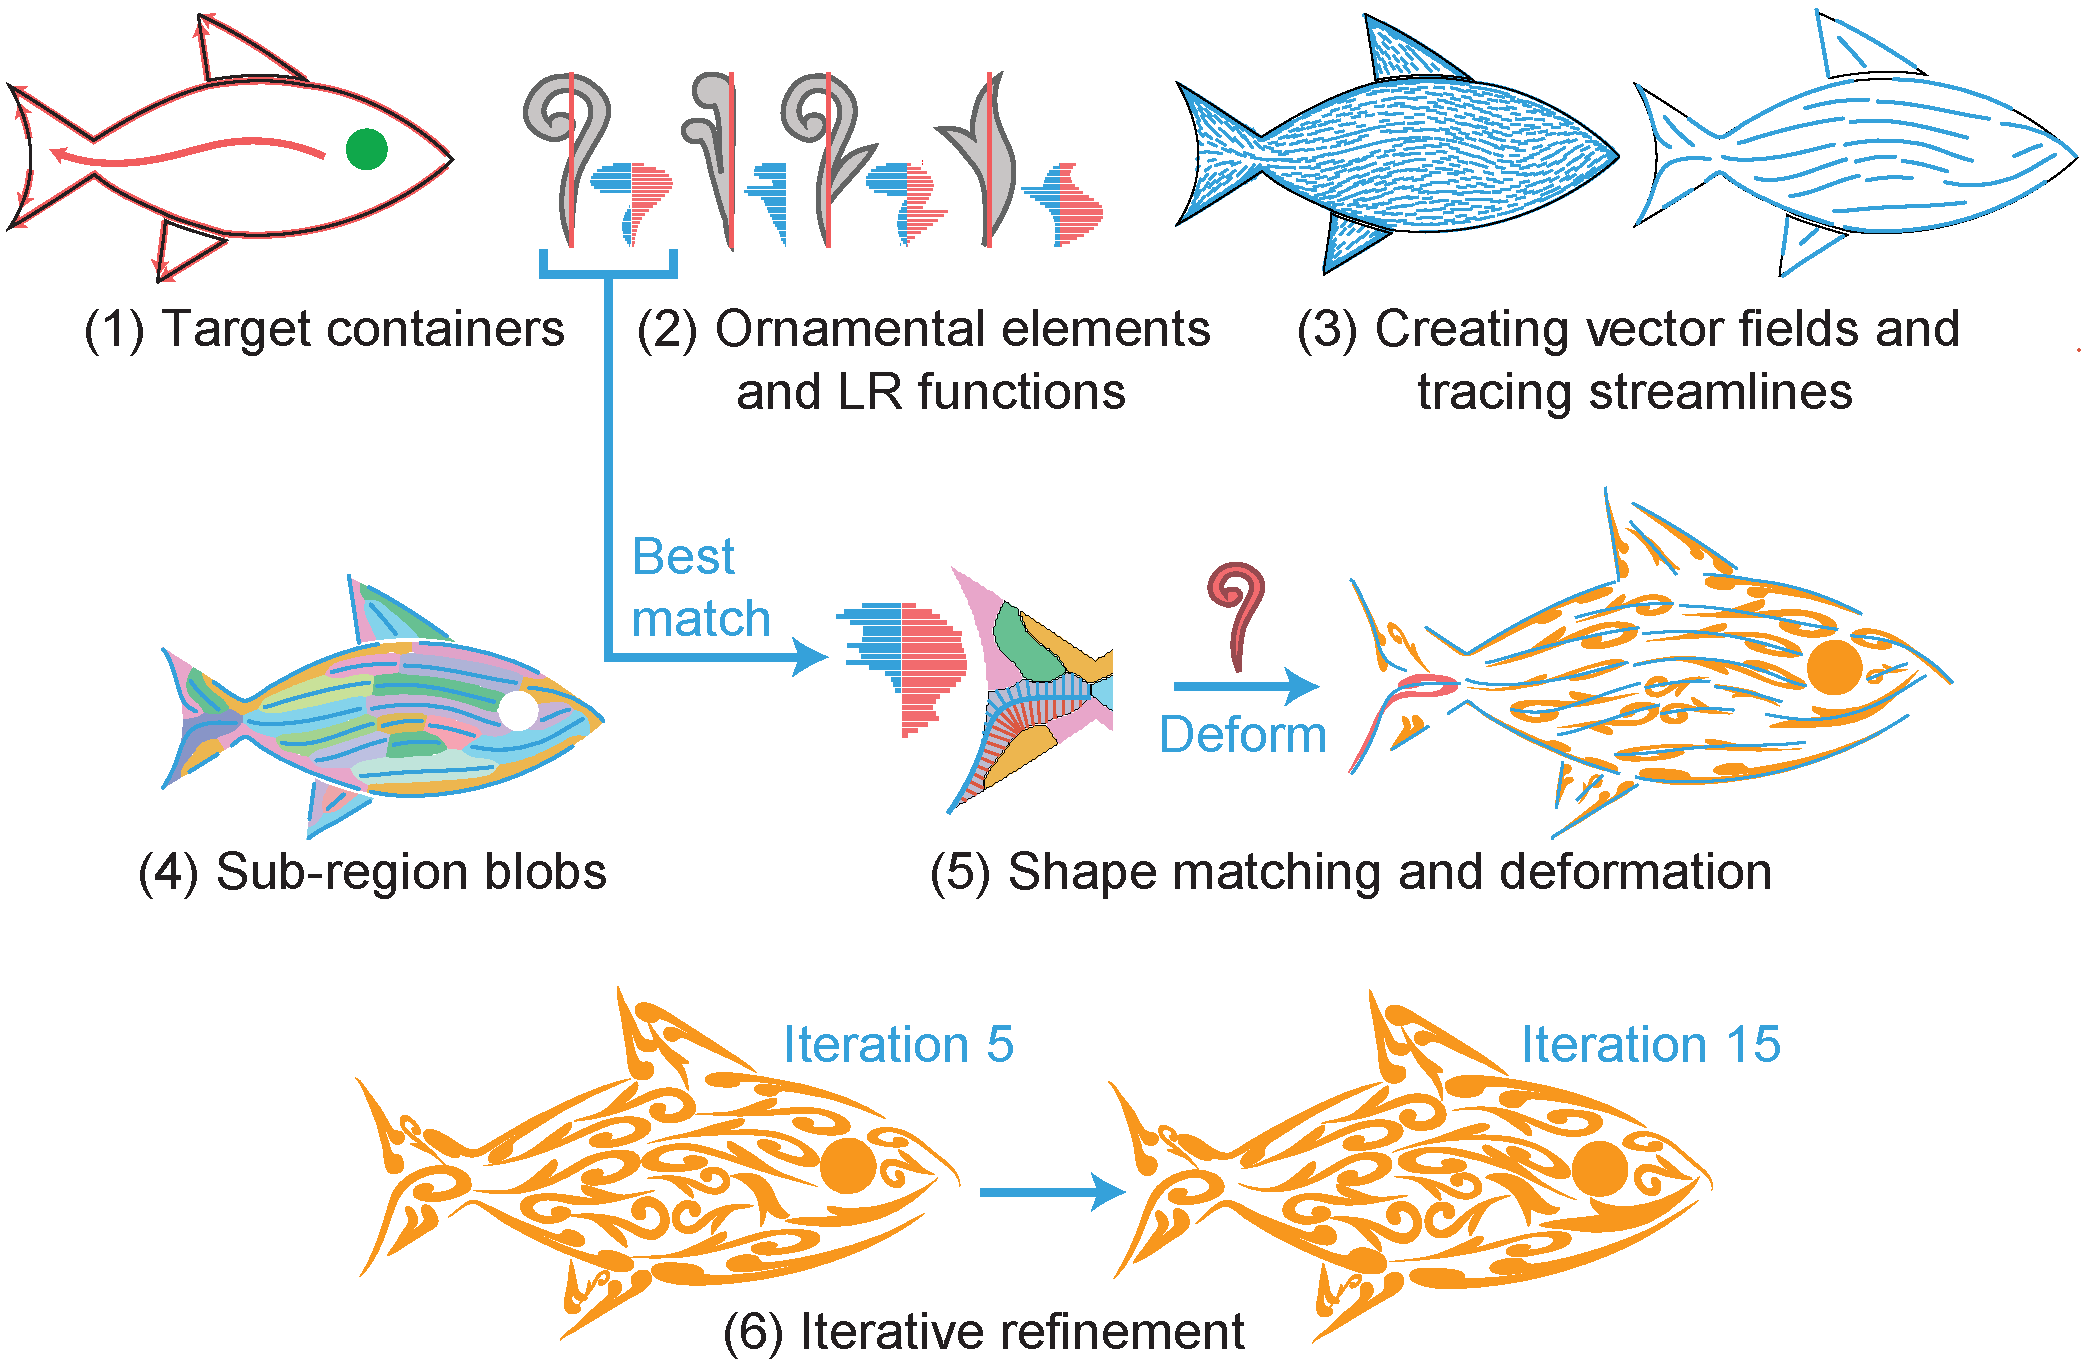
\includegraphics[width=1.0\textwidth]{figures/flowpak/pipeline.pdf} 
\caption[FLOWPAK pipeline]
{\label{fig_flowpak_pipeline} 
A visualization of the steps in our ornamental packing algorithm.
The input containers are shown as three black outlines in (1): the body
and two fins.  They are annotated with directional guides in red and fixed elements (in this 
case, the eye) in green.  The steps in the algorithm follow the
description at the beginning of Section~\ref{flowpak_approach}.
}
\end{figure}

%%%%%%%%%%%%%%%%%%%%%%%%%%%%%%%%%%%%%%%%%%%%%%%%%%%%%%%%%%
%%%%%%%%%%%%%%%%%%%%%%%%%%%%%%%%%%%%%%%%%%%%%%%%%%%%%%%%%%
\subsection{Target Containers}
\label{flowpak_target_containers}
%%%%%%%%%%%%%%%%%%%%%%%%%%%%%%%%%%%%%%%%%%%%%%%%%%%%%%%%%%
%%%%%%%%%%%%%%%%%%%%%%%%%%%%%%%%%%%%%%%%%%%%%%%%%%%%%%%%%%

The input diagram contains a set of target containers. Each is a single
closed curve defining an area
to be filled.  Most non-trivial examples include more than one target
container.  For the most part, our algorithm fills each container separately,
and so the following explanation is given in terms of a single container.
Containers will later be merged in the iterative refinement step.

The artist has the option of including a set of fixed elements that
we copy directly into the final result. The following sections
include descriptions of how the fixed elements affect the filling
algorithm.

%input\_size
We define \newtext{$l_\mathrm{canvas}$ to be the canvas size, which is the maximum of the combined width or height of all the
target containers and fixed elements as laid out by the artist.}
This value will be used to set various parameters in the synthesis process.

%%%%%%%%%%%%%%%%%%%%%%%%%%%%%%%%%%%%%%%%%%%%%%%%%%%%%%%%%%
%%%%%%%%%%%%%%%%%%%%%%%%%%%%%%%%%%%%%%%%%%%%%%%%%%%%%%%%%%
\subsection{Ornamental Elements and LR functions}
\label{flowpak_ornamental_element_and_lr_functions}
%%%%%%%%%%%%%%%%%%%%%%%%%%%%%%%%%%%%%%%%%%%%%%%%%%%%%%%%%%
%%%%%%%%%%%%%%%%%%%%%%%%%%%%%%%%%%%%%%%%%%%%%%%%%%%%%%%%%%

An ornamental element is defined as one or more closed curves.  Our placement method will
eventually deform copies of the element (Section~\ref{flowpak_shape_matching_and_deformation}) 
using a simple skeletal stroke algorithm~\cite{Hsu1993},
so each element must be annotated with a straight spine to guide the deformation.  The spine
does not need to go through the centre of the element---it can be anywhere.

We define two classes of elements: a \newtext{\textit{two-sided element}} extends across
both sides of its
spine, and a \newtext{\textit{one-sided element}} lies entirely on one side of its spine.
Figure~\ref{ornamental_shapes_fig} shows examples of \newtext{two-sided and one-sided elements}.  
If the input to our algorithm includes direction guides that coincide with target container boundaries,
the placement method will align \newtext{one-sided elements} along these boundaries.  
\newtext{The alignment of one-sided elements will visually reinforce
container boundaries, as shown in our results.}

%If \nnewtext{one-sided elements} have edges that closely follow their spines, they will visually reinforce
%container boundaries, as shown in our examples.

We define a simple shape descriptor called an \textit{LR function}
that will be used in
Section~\ref{flowpak_shape_matching_and_deformation} to choose which element to place in a particular location. 
Inspired by the work of Gal et al.~\cite{Gal2007A}, we sample the element's
spine at $n$ locations and at each location determine how far the ornament extends to the
left and right of the spine. \newtext{The LR function is the set $\{L, R\}$ where $L=\{\ell_1,\ldots,\ell_{n_\mathrm{f}}\}$
is the left function and $R=\{r_1,\ldots,r_{n_\mathrm{f}}\}$ is the right function. The number of samples is denoted by $n_\mathrm{f}$.}

The LR function is made scale-invariant by normalizing its
domain and range to $[0,1]$.  Note that swapping the $L$ and $R$ functions
corresponds to reflecting the element across its spine, and reversing each
of $L$ and $R$ corresponds to reflecting the element along its spine.  We
will consider all four combinations of these two reflections when placing 
an element in a blob (Section~\ref{flowpak_subregion_blobs}),
in order to achieve the best possible fit.

Intuitively, LR functions give an approximate area an ornamental element can claim.
Figure~\ref{ornamental_shapes_fig} 
shows elements with their left values
in blue and their right values in red. We have found that \newtext{$n_\mathrm{f} = 100$} gives sufficient
granularity for our algorithm.

%FFFFFFFFFFFFFFFFFFFFFFFFFFFFFFFFFFFFFFFFFFFFF
\begin{figure}
\centering
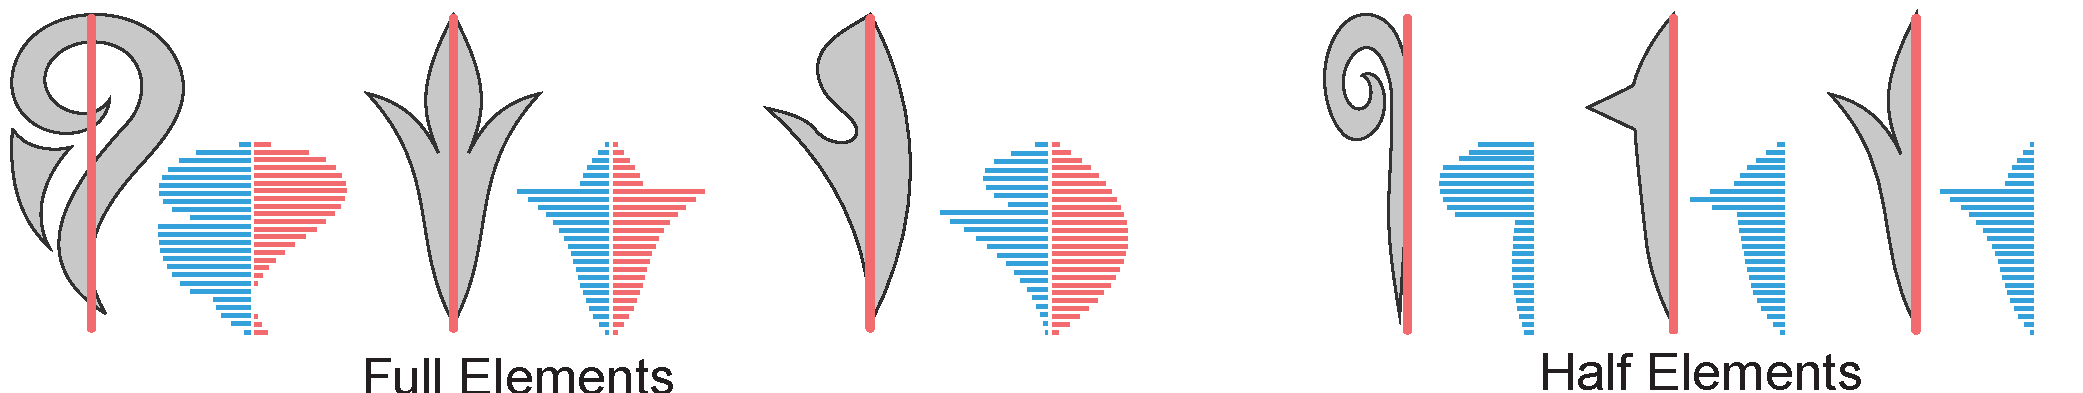
\includegraphics[width=1.0\textwidth]{figures/flowpak/ornaments.pdf}
\caption[Ornamental elements and their LR functions]
{\label{ornamental_shapes_fig}
Ornamental elements and their LR functions. \newtext{Two-sided elements} have non-empty
left and right sides, while \newtext{one-sided elements} have only one non-empty side. 
We normalize the LR functions to a unit square.}
\end{figure}

%%%%%%%%%%%%%%%%%%%%%%%%%%%%%%%%%%%%%%%%%%%%%%%%%%%%%%%%%%
%%%%%%%%%%%%%%%%%%%%%%%%%%%%%%%%%%%%%%%%%%%%%%%%%%%%%%%%%%
\subsection{Creating Vector Fields and Tracing Streamlines}
\label{flowpak_creating_vector_fields_and_tracing_streamlines}
%%%%%%%%%%%%%%%%%%%%%%%%%%%%%%%%%%%%%%%%%%%%%%%%%%%%%%%%%%
%%%%%%%%%%%%%%%%%%%%%%%%%%%%%%%%%%%%%%%%%%%%%%%%%%%%%%%%%%

To implement the flow principle described in the introduction, we fill each target
container with a vector field, constrained by the direction guides in that container.

We sample the directional guides $D = \{ d_{1}, d_{2}, ... , d_{n_\mathrm{d}}\}$  
and use the tangent at every sampled point as a directional constraint.
We then construct a vector field using the \newtext{\mbox{$1$-RoSy} algorithm}
of Palacios and Zhang~\cite{Palacios2007}.  Note that, as shown in 
Step~3 of Figure~\ref{fig_flowpak_pipeline},
fixed elements do not affect the vector field.  
The artist can include directional guides to guide the vector field around fixed elements if desired.

\newtext
{
The next step is to trace streamlines in the vector field, guided by three input parameters:
\begin{packeddescriptions}
\item[\newtext{$s_\mathrm{gap}$}] is the desired space between streamlines;
\item[\newtext{$s_\mathrm{max}$}] is the maximum desired streamline length; and
\item[\newtext{$s_\mathrm{min}$}] is the minimum desired streamline length.   
\end{packeddescriptions}
Because we will ultimately place elements along streamlines without overlap, \newtext{$s_\mathrm{gap}$} determines
the approximate width of the placed elements, and \newtext{$s_\mathrm{max}$} the maximum length.  We also derive
a value \newtext{$s_\mathrm{stop}$} that prevents streamlines from coming too close to each other; in our implementation we
compute \newtext{$s_\mathrm{stop} = 0.8\,s_\mathrm{gap}$}.
}

We adapt the streamline tracing algorithm of Jobard and Lefer~\cite{Jobard1997}.
First we generate a set of potential seed points $P = \{ \bm{p_{1}}, \bm{p_{2}}, ... , \bm{p_{n_\mathrm{p}}}\}$  by
densely resampling the target container boundary $T$ and the directional guides in $D$.
We use a sampling distance of \newtext{$0.005\,l_\mathrm{canvas}$}.
The first streamline $s$ is generated by randomly removing a seed point from $P$ and following
the vector field until one of the following conditions holds:

\begin{enumerate}
\item the length of $s$ would exceed \newtext{$s_\mathrm{max}$}.
\item $s$ would come within \newtext{$s_\mathrm{stop}$} of another streamline.
\item $s$ would cross $T$, leaving the container.
\item $s$ would cross the boundary of a fixed element.
\end{enumerate}


If the length of $s$ is less than \newtext{$s_\mathrm{min}$}, we discard it. Otherwise we sample 
$s$, again using \newtext{$0.005\,l_\mathrm{canvas}$}, and at each point generate two more
potential seeds that are \newtext{$s_\mathrm{gap}$} away from $s$ on either side. If a seed is
inside the container, we add it to $P$.  The process is repeated until $P$ is empty.
Note that the \newtext{$s_\mathrm{stop}$} distance test combined with the \newtext{$s_\mathrm{min}$} length
test imply that many attempts to form streamlines will stop immediately,
especially as the container fills with streamlines.

\begin{figure}
\centering

\includegraphics[width=1.0\textwidth]{figures/flowpak/streamline_tracing.pdf}
\caption[The streamline tracing process]
{\label{streamline_tracing}
The streamline tracing process. The first streamline $s_1$ always begins
on a directional guide or the container boundary.  Subsequent streamlines begin
on the container boundary, a directional guide, or at a point that is 
\newtext{$s_\mathrm{gap}$} away from a previous streamline.}
\end{figure}

Figure~\ref{streamline_tracing} shows the creation process, and 
Algorithm~\ref{tracing_streamlines} shows the pseudocode.
The sort function \textsc{Sort}$(P)$ orders the points in $P$ according to their distance from the
boundary $T$ and the directional guides in $D$, with closer points first and equally distant
points ordered randomly. Because the initial points are all on $T$ or on a path in $D$, their
sort value is zero, and they will be processed before any derived points. 



\begin{algorithm}
\caption{Tracing Streamlines} 
\label{tracing_streamlines}
\begin{algorithmic} 
\STATE Create a seed list $P = \{ \bm{p_{1}}, \bm{p_{2}}, ... , \bm{p_{n_\mathrm{p}}}\}$ 
       by uniformly resampling
\STATE \hskip\algorithmicindent $T$ and the guides in $D$.
\STATE Create an empty set $S$ of streamlines.
\STATE Randomly order the elements of $P$.
\WHILE {$P$ is not empty}
  \STATE Generate a new streamline $s$ from $\bm{p_{1}}$.
  \STATE Remove $\bm{p_{1}}$ from $P$.
  \IF {$s$ is longer than \newtext{$s_\mathrm{min}$}}
    \STATE Add $s$ to $S$.
    \STATE Create seed points that are \newtext{$s_\mathrm{gap}$} away from $s$ and
	\STATE \hskip\algorithmicindent add them to $P$.
    \STATE \textsc{Sort}$(P)$.
  \ENDIF
\ENDWHILE
\end{algorithmic}
\end{algorithm}



%FFFFFFFFFFFFFFFFFFFFFFFFFFFFFFFFFFFFFFFFFFFFF


%%%%%%%%%%%%%%%%%%%%%%%%%%%%%%%%%%%%%%%%%%%%%%%%%%%%%%%%%%
%%%%%%%%%%%%%%%%%%%%%%%%%%%%%%%%%%%%%%%%%%%%%%%%%%%%%%%%%%
\subsection{Sub-Region Blobs}
\label{flowpak_subregion_blobs}
%%%%%%%%%%%%%%%%%%%%%%%%%%%%%%%%%%%%%%%%%%%%%%%%%%%%%%%%%%
%%%%%%%%%%%%%%%%%%%%%%%%%%%%%%%%%%%%%%%%%%%%%%%%%%%%%%%%%%

To assist in choosing which element to place along each streamline, we first
subtract the areas of any fixed elements from the target container. We then
construct an approximate generalized Voronoi diagram of the interior
using the method of Osher and Sethian~\cite{Osher1988}.
The streamlines are then extended at each end, following the vector field, until
they encounter the boundaries of their Voronoi regions.
We call the area around each streamline a \textit{sub-region blob}.
Step~4 of Figure~\ref{fig_flowpak_pipeline} 
\newtext{shows the blobs of the fish.}

We then compute an LR function for each blob as described in Section~\ref{flowpak_ornamental_element_and_lr_functions},
using the streamline as the spine. Because the streamline is not usually straight, we 
compute the left and right distances along the normals to the streamline. The LR function approximates
the blob's shape if the streamline were to be straightened.

%%%%%%%%%%%%%%%%%%%%%%%%%%%%%%%%%%%%%%%%%%%%%%%%%%%%%%%%%%
%%%%%%%%%%%%%%%%%%%%%%%%%%%%%%%%%%%%%%%%%%%%%%%%%%%%%%%%%%
\subsection{Shape Matching and Deformation}
\label{flowpak_shape_matching_and_deformation}
%%%%%%%%%%%%%%%%%%%%%%%%%%%%%%%%%%%%%%%%%%%%%%%%%%%%%%%%%%
%%%%%%%%%%%%%%%%%%%%%%%%%%%%%%%%%%%%%%%%%%%%%%%%%%%%%%%%%%

The next step is to place an ornamental element in each blob.  We choose which element
to place in the blob by finding the element that minimizes a sum of least squares distance, defined as
%\vspace{-4pt}
\begin{equation}
\sum_{i=1}^{N} (\alpha_{li} - \beta_{li})^2 + \sum_{i=1}^{N} (\alpha_{ri} - \beta_{ri})^2
\end{equation}
where
%\vspace*{-4pt}
\begin{conditions}
\alpha_{l}\enspace & the element \newtext{$L$ function};\\
\alpha_{r} &  the element \newtext{$R$ function}; \\   
\beta_{l}  &  the blob \newtext{$L$ function}; and \\
\beta_{r}  &  the blob \newtext{$R$ function}.
\end{conditions}
%\vspace{-4pt}

Every element can be placed in one of four orientations, by optionally 
incorporating reflections across and along its spine.  These reflections
correspond, respectively, to swapping the $L$ and $R$ functions and reversing
them.  When comparing the LR functions for an element and a blob, we compute
the least squares distances for all four orientations and choose the 
orientation with the smallest distance.  Note that this matching method
\newtext{will naturally place} \newtext{one-sided elements} along streamlines that follow container
boundaries, visually reinforcing the overall shape.

We investigated alternatives for shape matching, using an approach
discussed by Gal et al. \cite{Gal2007B} that tries to fill a sub-region
blob as much as possible, with heavy penalties if a part of an
element protrudes outside the boundary of the blob. However, we found
this computation to be more expensive without providing significant
advantages over our LR functions.

Once we have chosen an element, we place it along the streamline using a
simple skeletal stroke algorithm~\cite{Hsu1993}. We uniformly scale the element's width
to make it as wide as possible while still staying inside the blob
(Figure~\ref{shape_deformation}).

%FFFFFFFFFFFFFFFFFFFFFFFFFFFFFFFFFFFFFFFFFFFFF
\begin{figure}
\centering

\includegraphics[width=1.0\textwidth]{figures/flowpak/shape_deformation.pdf}
\caption[Element deformation]
{\label{shape_deformation}
The deformation process bends the element along the streamline and
scales it to fit inside the blob.}
\end{figure}

%%%%%%%%%%%%%%%%%%%%%%%%%%%%%%%%%%%%%%%%%%%%%%%%%%%%%%%%%%
%%%%%%%%%%%%%%%%%%%%%%%%%%%%%%%%%%%%%%%%%%%%%%%%%%%%%%%%%%
\subsection{Iterative Refinement}
\label{flowpak_iterative_refinement}
%%%%%%%%%%%%%%%%%%%%%%%%%%%%%%%%%%%%%%%%%%%%%%%%%%%%%%%%%%
%%%%%%%%%%%%%%%%%%%%%%%%%%%%%%%%%%%%%%%%%%%%%%%%%%%%%%%%%%

%It's been a while since we've thought about multiple containers. This section could use another sentence or two as an opener. 
%Remind us that we've created an initial layout of flow-guided elements in each distinct container. Now we merge all the containers and...

\newtext
{
\newtext{The previous steps} produce an initial arrangement \newtext{consisting of a packing of} 
flow-guided elements in each distinct container.
We now merge all the containers and all elements within them,
allowing elements from different containers to interact with each other 
in an iterative manner.
}

%We now refine the overall composition in an iterative process.  We perform
%this part of the algorithm globally, by merging all containers and allowing the
%elements within them to interact.

\nnewtext{The refinement process aims to reduce the amount of negative space and make it
more even by growing and shifting the placed ornamental elements. 
We improve the placement of each element as much as possible before moving on to the next.}
\deadtext{It would be possible to use a greedy approach, improving the placement of each element as much
as possible before moving on to the next, However, we have found that gradually
improving the placement of all elements leads to a more even result.}
Each refinement iteration has two phases.
First, we shift the streamlines to more accurately follow the space that is available,
as shown in Figure~\ref{shift_streamline}. After shifting, we recalculate the LR function
for the blob to reflect the new position, and repeat a variant of the
element placement process
that allows the elements to rotate slightly in their space.
Second, we expand each blob to allow it to use adjacent space that is not 
filled with another element, as shown in Figure~\ref{stretch_ornament}.

Each refinement iteration considers the blobs in increasing order of 
placed element area, allowing smaller elements to grow more.   While each step
usually results in a larger placed element, some
configurations can result in a smaller one. We only accept the new element if its
area is no smaller than $\alpha$ times its old area, where $\alpha$ is a growth tolerance
that we set to $0.9$. Elements therefore have some freedom to grow or
shrink, in the search for more globally even spacing.

\newtext{
The rest of this section gives the implementation details of the refinement process
and Algorithm~\ref{iterative_refinement_algorithm} summarizes the overall method.}
We have found that 15 iterations suffice for most designs.
Note that in Algorithm~\ref{iterative_refinement_algorithm}, the variable
$E$ is the list of placed, distorted ornamental elements, and
not the set of prototype elements discussed earlier.

\begin{algorithm}
\caption{Iterative Refinement} 
\label{iterative_refinement_algorithm}
\begin{algorithmic} 
\REQUIRE $E = \{ e_{1}, e_{2},... , e_{n_\mathrm{e}} \}$ as the ornamental element list. 
\REQUIRE $S = \{ s_{1}, s_{2},... , s_{n_\mathrm{s}} \}$ as the streamline list.
\REQUIRE $B = \{ b_{1}, b_{2},... , b_{n_\mathrm{b}} \}$ as the blob list.
\REQUIRE $\alpha$ as the growth tolerance
\REQUIRE $t$ as the number of iterations
\FOR {$t$ times}

  \STATE Sort $E$, $S$, and $B$ by \textsc{Area}$(e_{i})$ (smallest first)
  \FOR {Element $e_{i}$ in $E$}
  	\STATE $s_{i}$ is the corresponding streamline of $e_{i}$
    \STATE Calculate $s'_{i}$ by \textbf{shifting} $s_{i}$.
    \STATE Recompute the LR function of $b_{i}$ to give $b'_{i}$
    \STATE Calculate $e'_{i}$ by \textbf{placing} $e_{i}$ inside $b'_{i}$
    \IF{$\textsc{Area}(e'_{i}) \times \alpha > \textsc{Area}(e_{i})$}
        \STATE $s_{i} \leftarrow s'_{i}$
        \STATE $b_{i} \leftarrow b'_{i}$
    	\STATE $e_{i} \leftarrow e'_{i}$ 
    \ENDIF
  \ENDFOR
  \STATE Sort $E$, $S$, and $B$ by \textsc{Area}$(e_{i})$ (smallest first)

  \FOR {Element $e_{i}$ in $E$}
  	\STATE $b_{i}$ is the corresponding blob of $e_{i}$
    \STATE Calculate $b'_{i}$ by \textbf{growing} $b_{i}$.
    \STATE Calculate $s'_{i}$ based on $b'_{i}$ 
    \STATE Calculate $e'_{i}$ by \textbf{placing} $e_{i}$ inside $b'_{i}$\
    \STATE $b_{i} \leftarrow b'_{i}$
    \IF{$\textsc{Area}(e'_{i}) \times \alpha > \textsc{Area}(e_{i})$}
        \STATE $s_{i} \leftarrow s'_{i}$
    	\STATE $e_{i} \leftarrow e'_{i}$ 
    \ENDIF
  \ENDFOR

\ENDFOR
\end{algorithmic}
\end{algorithm}





\textbf{Shifting Streamlines.}
There are two issues that keep the initial placement of elements from being
evenly
distributed. Our streamline placement method keeps streamlines apart,
but they may not be spaced completely evenly. More significantly, the
ornamental elements often have unbalanced left and right sides and concavities,
leading to extra space on one side or the other.  Our refinement process
shifts streamlines to address these problems.

The shifting process allows the endpoints of the streamline to move to the
left or the right relative to the streamline, depending on which side has more empty space.
This allows the streamline's element to become wider and fill more of the space
(Figure~\ref{shift_streamline}). It also gives the streamline room to
extend if its endpoints were too close to boundaries of other placed
elements.

\begin{figure}
 
\includegraphics[width=1.0\textwidth]{figures/flowpak/shift_streamline.pdf}
 \caption[Shifting a streamline]
 {\label{shift_streamline}
 Streamline shifting.
  We move the streamline's start and end points along 
  perpendiculars, stopping before intersecting neighbouring elements.}
\end{figure}


Given the endpoints $\bm{p_\mathrm{start}}$ and $\bm{p_\mathrm{end}}$, we 
calculate new endpoints $\bm{p'_\mathrm{start}}$ and $\bm{p'_\mathrm{end}}$.
We generate perpendicular
vectors to the left side and to the right side at each endpoint and construct
a line segment joining the points where the vectors intersect other placed elements.
We then move the endpoint of the streamline towards the midpoint of this
segment. To enforce the principle of gradual refinement, we do not allow the
endpoint to move more than $g_\mathrm{limit}$ units, where 
\newtext{$g_\mathrm{limit}=0.005\,l_\mathrm{canvas}$ (Recall that $l_\mathrm{canvas}$} is the \newtext{canvas size}
of the design as described in Section~\ref{flowpak_target_containers}).

We replace the streamline with a path joining
$\bm{p'_\mathrm{start}}$ and $\bm{p'_\mathrm{end}}$. Our goal
is to create a path that is smooth and does not deviate too much from the vector
field.  We calculate the shifted streamline by performing Dijkstra's
algorithm on a non-rectangular graph that respects the vector field
(Figure~\ref{dijkstra}), using a method similar to one by Xu and Mould~\cite{Xu2015} for
pathfinding in a vector field.

\begin{figure}

\includegraphics[width=1.0\textwidth]{figures/flowpak/dijkstra.pdf}
 \caption[Tracing a shortest path]
 {\label{dijkstra}
 \newtext{
 Tracing a shortest path using Dijkstra's algorithm.  We generate the 
 blue nodes by resampling and offsetting the blue streamline.
          The search directions at a node are shown with green arrows.}}
\end{figure}

To construct the graph, we begin by densely sampling the original
streamline with a distance of $0.25\,g_\mathrm{limit}$. We then duplicate
the points, offset to the left and right, again using $0.25\,g_\mathrm{limit}$.
The duplication is repeated until the graph extends to the left and right of the
streamline by a distance equal to the maximum left and right widths of the blob (i.e.,
the maximum values in an unnormalized version of the blob's LR function).

For a node, we check its $150$ nearest neighbours, 
considering only neighbours where the angle between the line into the current node and the line to the neighbour form an angle greater than $90^\circ$, thereby preventing
the streamline from backtracking.
The cost of an edge from \newtext{$\bm{p_a}$} to  \newtext{$\bm{p_b}$} is 

\begin{equation}
w = w_f (1 - f^p) + w_d \: D(s_i, \bm{p_a})
\end{equation}
where
\begin{conditions}
f                  & $(\bm{p_b} - \bm{p_a}) \cdot \bm{v}$; \\
\bm{v} 		   & \newtext{a sampled unit vector of the vector field at $\bm{p_a}$}; \\
s_i                & the original streamline; and \\   
D()\enspace        & a distance function between a polyline and a point.
\end{conditions}

In practice, we set $w_d = 0.1$, $w_f=1$, and $p = 3$.

After finding a set of points, we fit cubic B\'ezier curves using a method
devised by Schneider \cite{Schneider1990} and extend the path at both ends 
by following
the vector field until it intersects the edges of its blob. 




\textbf{Growing Blobs.} The growth process tries to enlarge each sub-region blob to
claim empty space.
Given a blob $b_{i}$, we calculate a larger blob $b'_{i}$ 
by offsetting its boundaries until they intersect other placed elements (Figure~\ref{stretch_ornament}).
To enforce gradual growth, the offset cannot be larger than $g_\mathrm{limit}$, where
\newtext{$g_\mathrm{limit}=0.005\,l_\mathrm{canvas}$.}

The value $g_\mathrm{limit}$ used in growing blobs and shifting streamlines limits the speed of
the refinement.  Making it larger would require fewer iterations to fill the available space,
but at a cost of elements growing less evenly. 

% ROTATING OR FLIPPING
\textbf{Element Placement.}
In the refinement process, we allow a more flexible element placement so that
the elements can fill more of their blobs.  We allow the element
to rotate by a small amount, up to ten degrees, before placing it, as shown in
Figure~\ref{rotate_ornament}. 
We generate rotated versions of $e_{i}$ 
with varying angles \newtext{$r_\mathrm{angle} = \pm \{1^{\circ}, 2^{\circ}, 3^{\circ}, ..., 10^{\circ}\}$}
and precompute LR functions for each. The shape matching algorithm
(Section~\ref{flowpak_shape_matching_and_deformation}) automatically choses the best rotation. It
can also choose to reflect the element across its spine, along its spine, or both (Figure~\ref{flip_shape}).

%FFFFFFFFFFFFFFFFFFFFFFFFFFFFFFFFFFFFFFFFFFFFF
\begin{figure}
\centering

\includegraphics[width=1.0\textwidth]{figures/flowpak/stretch.pdf}
\caption[Stretching an element]
{\label{stretch_ornament}
(a) An element with its sub-region blob shown in dashed blue line. Note that any blob is constrained by the neighbouring elements. 
(b) The dashed red line is the grown blob, which accommodates an enlarged element.}

\bigskip
\bigskip
% ROTATING OR FLIPPING
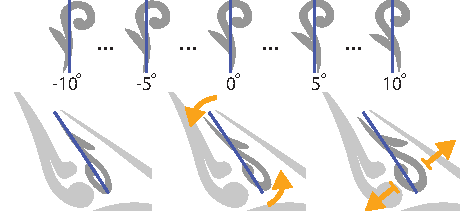
\includegraphics[width=1.0\textwidth]{figures/flowpak/rotate_ornament.pdf}
\caption[Rotating an element]
{\label{rotate_ornament}
\newtext{Left}: rotated versions of the original element. 
         The best rotation angle is chosen via least squares matching.
         \newtext{Right}: original, rotated, and enlarged versions of an element.}
\bigskip
\bigskip

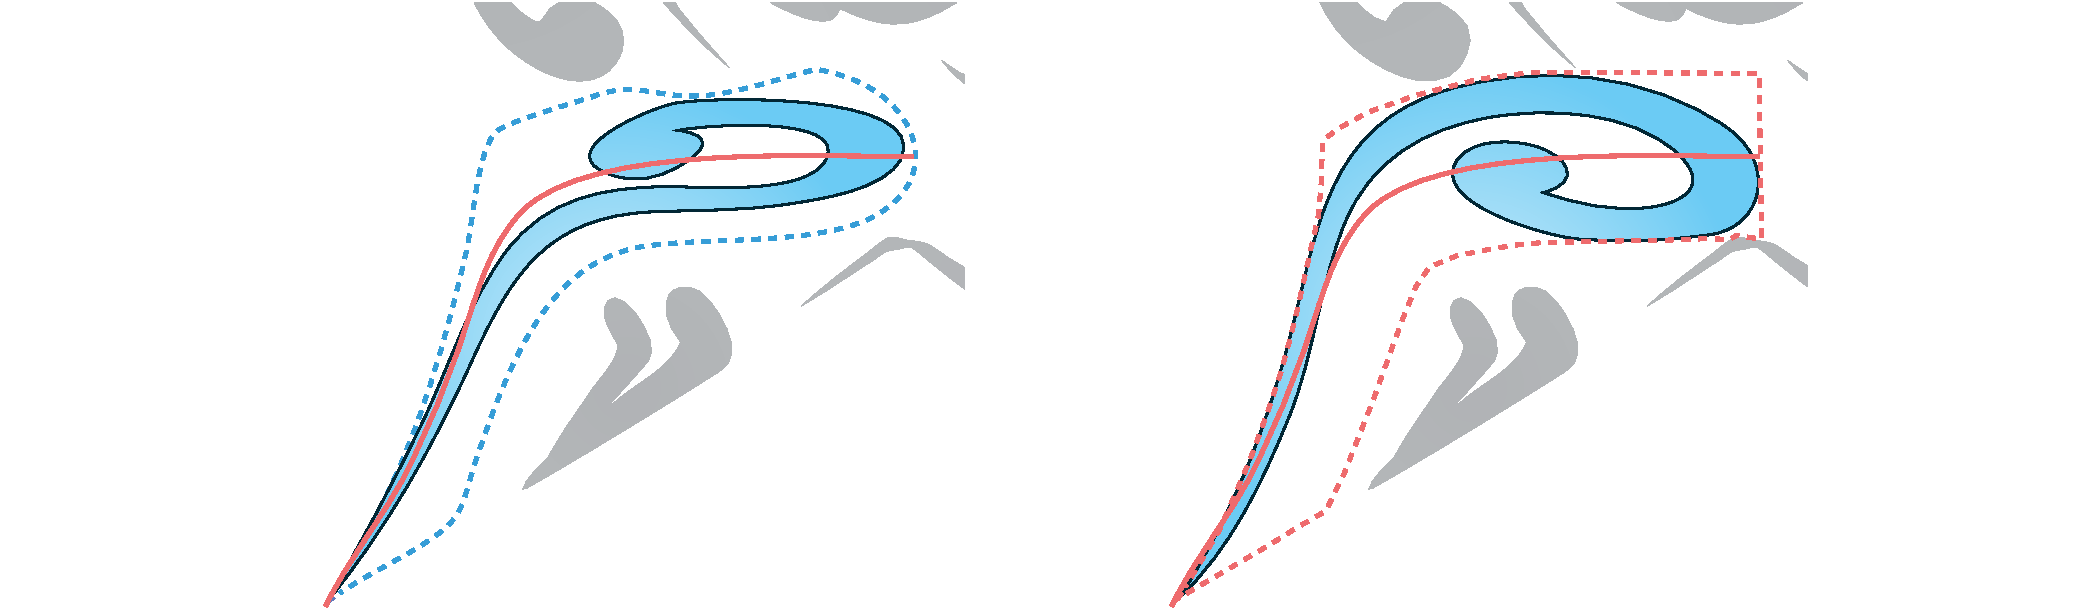
\includegraphics[width=1.0\textwidth]{figures/flowpak/flip.pdf}
\caption[Reflecting an element]
{\label{flip_shape}
An element that reflects across its spine during iterative refinement.
LR functions and least squares shape matching allow an element to reflect
across its spine, along its spine, or both.}
\end{figure}

%%%%%%%%%%%%%%%%%%%%%%%%%%%%%%%%%%%%%%%%%%%%%%%%%%%%%%%%%%
%%%%%%%%%%%%%%%%%%%%%%%%%%%%%%%%%%%%%%%%%%%%%%%%%%%%%%%%%%
\section{Implementation and Results}
\label{flowpak_implementation_and_results}
%%%%%%%%%%%%%%%%%%%%%%%%%%%%%%%%%%%%%%%%%%%%%%%%%%%%%%%%%%
%%%%%%%%%%%%%%%%%%%%%%%%%%%%%%%%%%%%%%%%%%%%%%%%%%%%%%%%%%



We design our containers and decorative elements in a vector graphics 
editor, and then use them as input to a C++ program that outputs final
placed elements in an SVG file.  We use the Clipper library~\cite{ClipperLib}
for calculation of LR functions and for testing polygon intersections 
during deformation and growth.
As a postprocess, we optionally smooth outlines and replace polygonal
paths with B\'{e}zier curves.
Finally, we apply colours and other treatments in an editor.

Our technique is fast except for the iterative refinement process,
which considers a large number of variations to the composition via
brute-force computation. On a computer with an Intel i7-4790K processor at 4.0 Ghz,
 15 iterations
of refinement on a packing of 50 elements takes about an hour.  Our
software is not intended to run interactively; still, we believe the
performance could be improved significantly through the use of more
sophisticated 2D geometric data structures \newtext{such as uniform grids or quadtrees}.

We tested our approach using a variety of container shapes, based mostly
on animals, and many different ornamental elements with varying amounts
of geometric complexity.
In Figure~\ref{fig_lion_unicorn}, we show two packings of a lion and a unicorn.
Each packing is generated with only a set of four elements.
The packings demonstrate that FLOWPAK is able to pack and deform
elements inside the containers.
In Figure~\ref{result_rhino},
we show a packing of a rhinoceros with simple teardrop elements
that demonstrates the variety we achieve in shape and curvature.
We use more complex leaf elements on the bear in 
Figure~\ref{result_bear_leaves}, and
adjust the tracing parameters to obtain shorter placed elements. 
We also process the placed elements to create a distressed look.

The packing of a cat in Figure~\ref{result_cat} demonstrates 
a symmetric packing with a fur contour. 
We \newtext{compute only} the left part and reflect the result.
The elements around the cheeks and the chin extend outward, not following the boundary, and creating the appearance of fur.

We experimented with two extensions to our pipeline, 
which could enhance its aesthetic value and flexibility.
First, in Figure~\ref{result_dog} we allow the user to draw 
\textit{fixed spines} in addition to fixed elements.  These fixed
spines act like pre-placed streamlines, which will be assigned blobs
and then elements.  However, they are not required to follow the
surrounding vector field, and are not shifted during the refinement
process.  Fixed spines are used in Figure~\ref{result_dog} for the 
flower petals in the torso and the paws.
Second, in Figure~\ref{result_bear_offset} we construct explicit new shapes
(drawn in brown)
to fill the negative space between placed elements (in black), 
by computing offset polygons from the negative space between elements. 
The result is a distinct and appealing style.  

Finally, we asked an artist to draw containers and decorative elements.
The result is the bird design shown in Figure~\ref{bird_square}.
The artist requested that different elements and densities be used in 
different container regions; the result has sparse ``Y'' elements in 
the breast and head, and denser ``O'' elements in the wings. The artist was pleased with the \newtext{result}.


%FFFFFFFFFFFFFFFFFFFFFFFFFFFFFFFFFFFFFFFFFFFFF



%%%%%%%%%%%%%%%%%%%%%%%%%%%%%%%%%%%%%%%%%%%%%%%%%%%%%%%%%%
%%%%%%%%%%%%%%%%%%%%%%%%%%%%%%%%%%%%%%%%%%%%%%%%%%%%%%%%%%
\section{Conclusions and Future Work}
\label{flowpak_conclusions}
%%%%%%%%%%%%%%%%%%%%%%%%%%%%%%%%%%%%%%%%%%%%%%%%%%%%%%%%%%
%%%%%%%%%%%%%%%%%%%%%%%%%%%%%%%%%%%%%%%%%%%%%%%%%%%%%%%%%%

\newtext
{
We presented FLOWPAK, a method to create ornamental packings
in which the elements \newtext{are} oriented and deformed to give a sense of visual flow to the final composition.
Our implementation computed a vector field based on user strokes,
constructed streamlines that conform to the vector field, and placed an
element over each streamline. An iterative refinement process then
shifted and stretched the elements to improve the composition.
}

\newtext
{
\newtext{We see two natural opportunities for} improving FLOWPAK.
\newtext{First, we would like to generate streamlines with higher curvatures, like u-turns.
However, these streamlines} could unpleasantly fold the decorative elements. 
This could be solved with a folding avoidance algorithm~\cite{Asente2010}.
Second, we would like to experiment with a procedure for element placements that can backtrack to previous configurations, 
as demonstrated by \newtext{Jigsaw Image Mosaics}~\cite{Kim2002}. 
This way, we can achieve a better configuration \newtext{with less iterative refinement}.
}
\begin{figure}
\centering
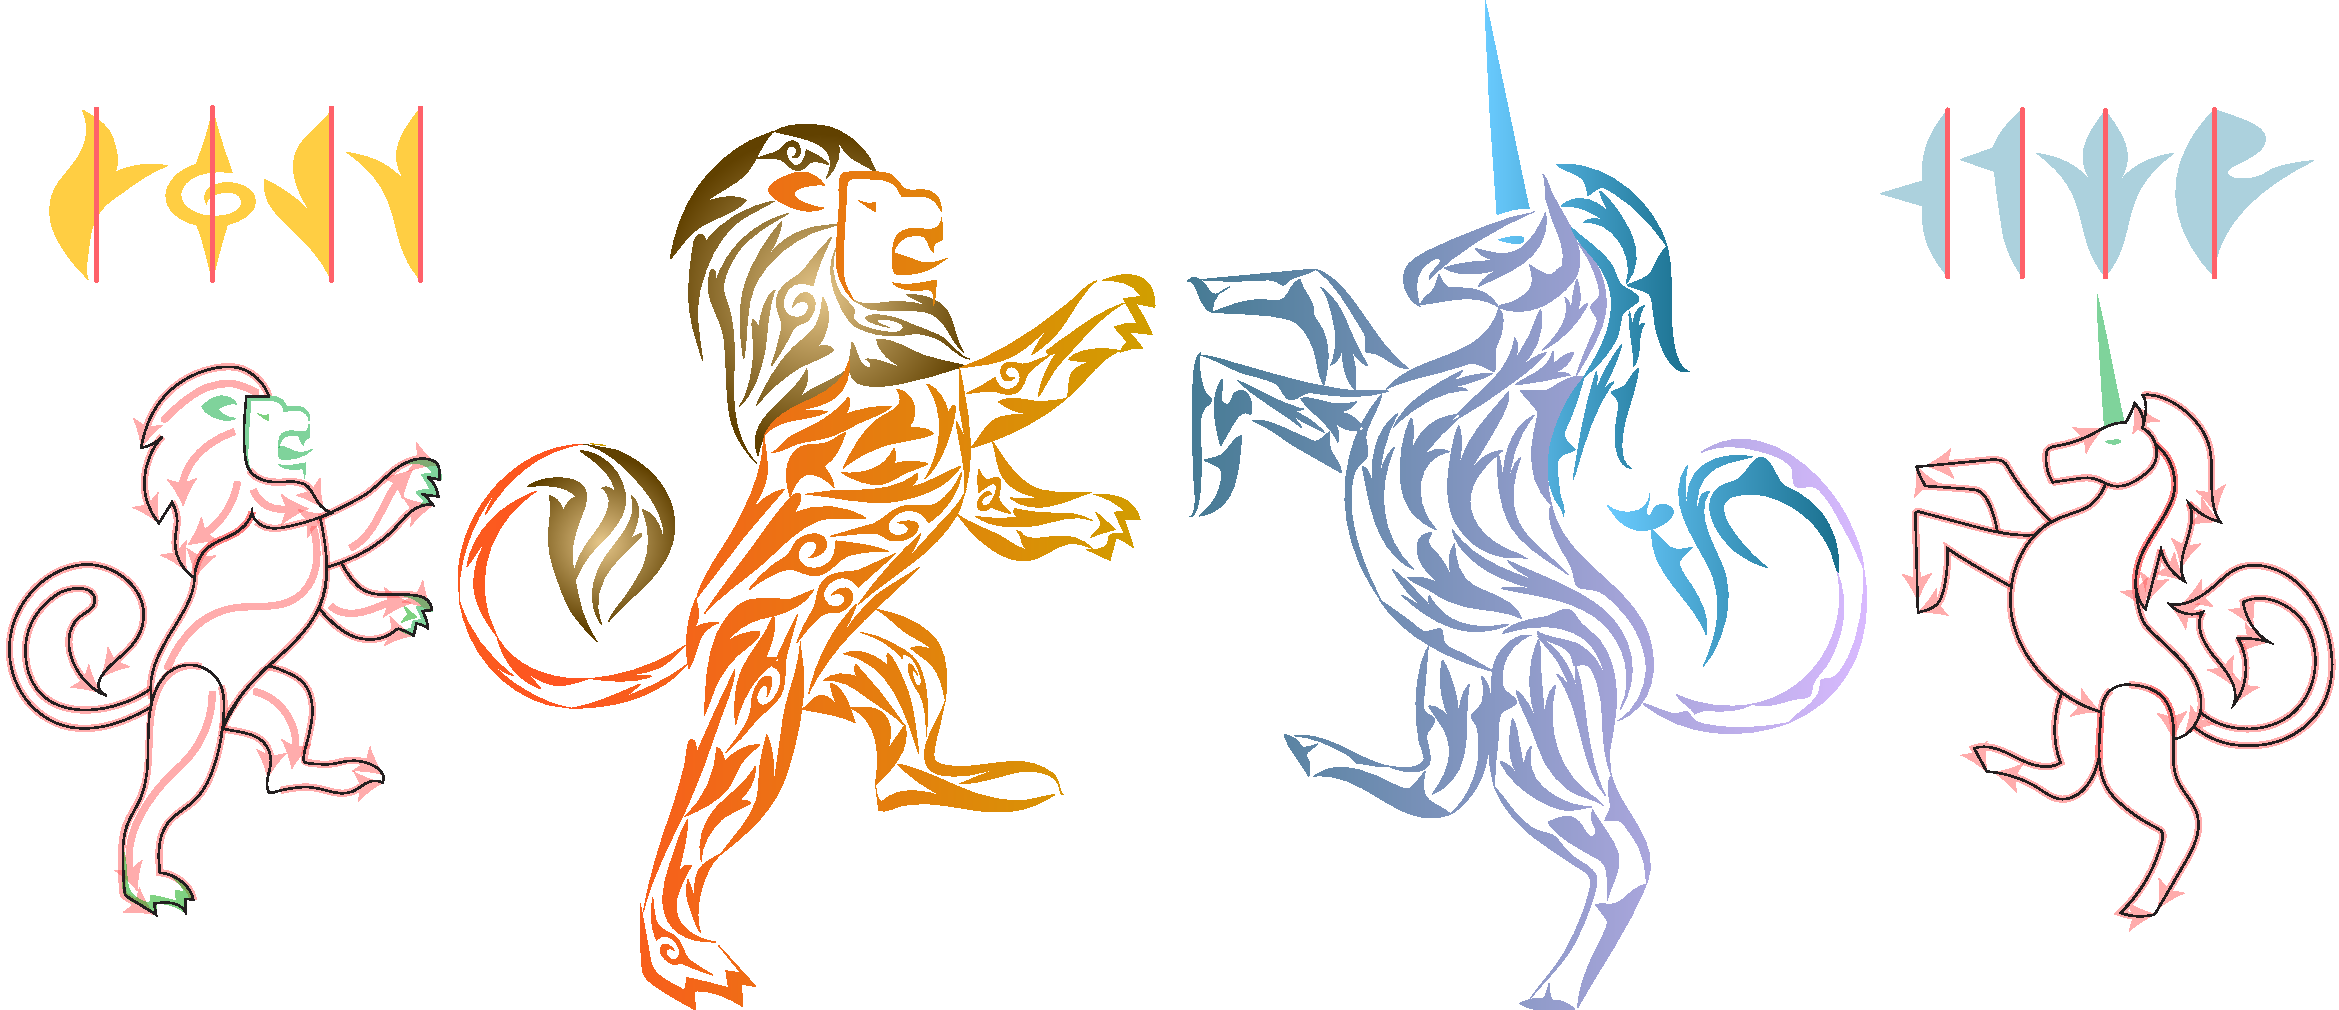
\includegraphics[width=1.0\textwidth]{figures/flowpak/lion_unicorn.pdf} 
\caption[Packings of lion and unicorn]
{\label{fig_lion_unicorn} 
\newtext{Ornamental packings of a lion and a unicorn.
The diagram next to each animal shows a set of four ornamental
elements used in the packing (top) and the annotated
container regions (bottom).  
%Each ornamental element has a
%red spine that is used to deform it along a streamline.  In
%the containers, black curves represent boundaries, red
%curves with arrows represent directional guides, and green
%curves are fixed elements copied into the final design.
The colours in the final rendering were added manually.}
}
\end{figure}

%FFFFFFFFFFFFFFFFFFFFFFFFFFFFFFFFFFFFFFFFFFFFFFFFFFFFFFFFFFFF
\begin{figure}
\centering
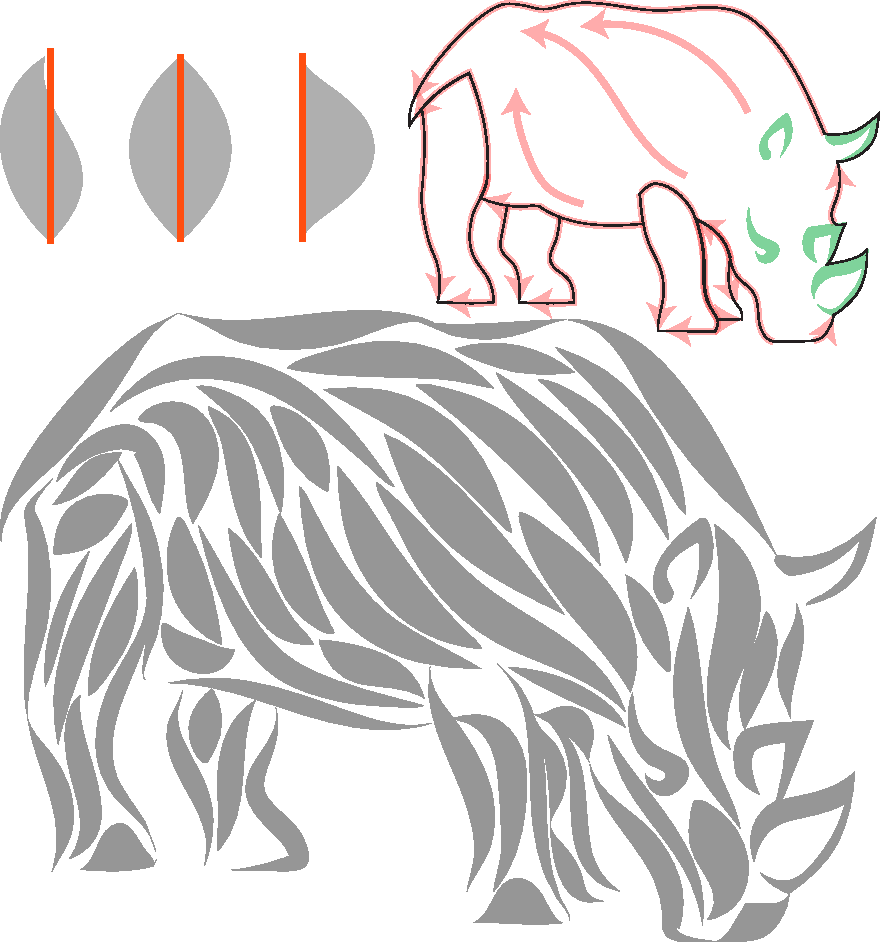
\includegraphics[width=1.0\textwidth]{figures/flowpak/result_02.pdf} %RHINO
\caption[A packing of a rhinoceros]
{\label{result_rhino}
A packing of a rhinoceros.  Simple teardrop-shaped 
elements lead to variety in size and curvature.}
\end{figure}
\begin{figure}
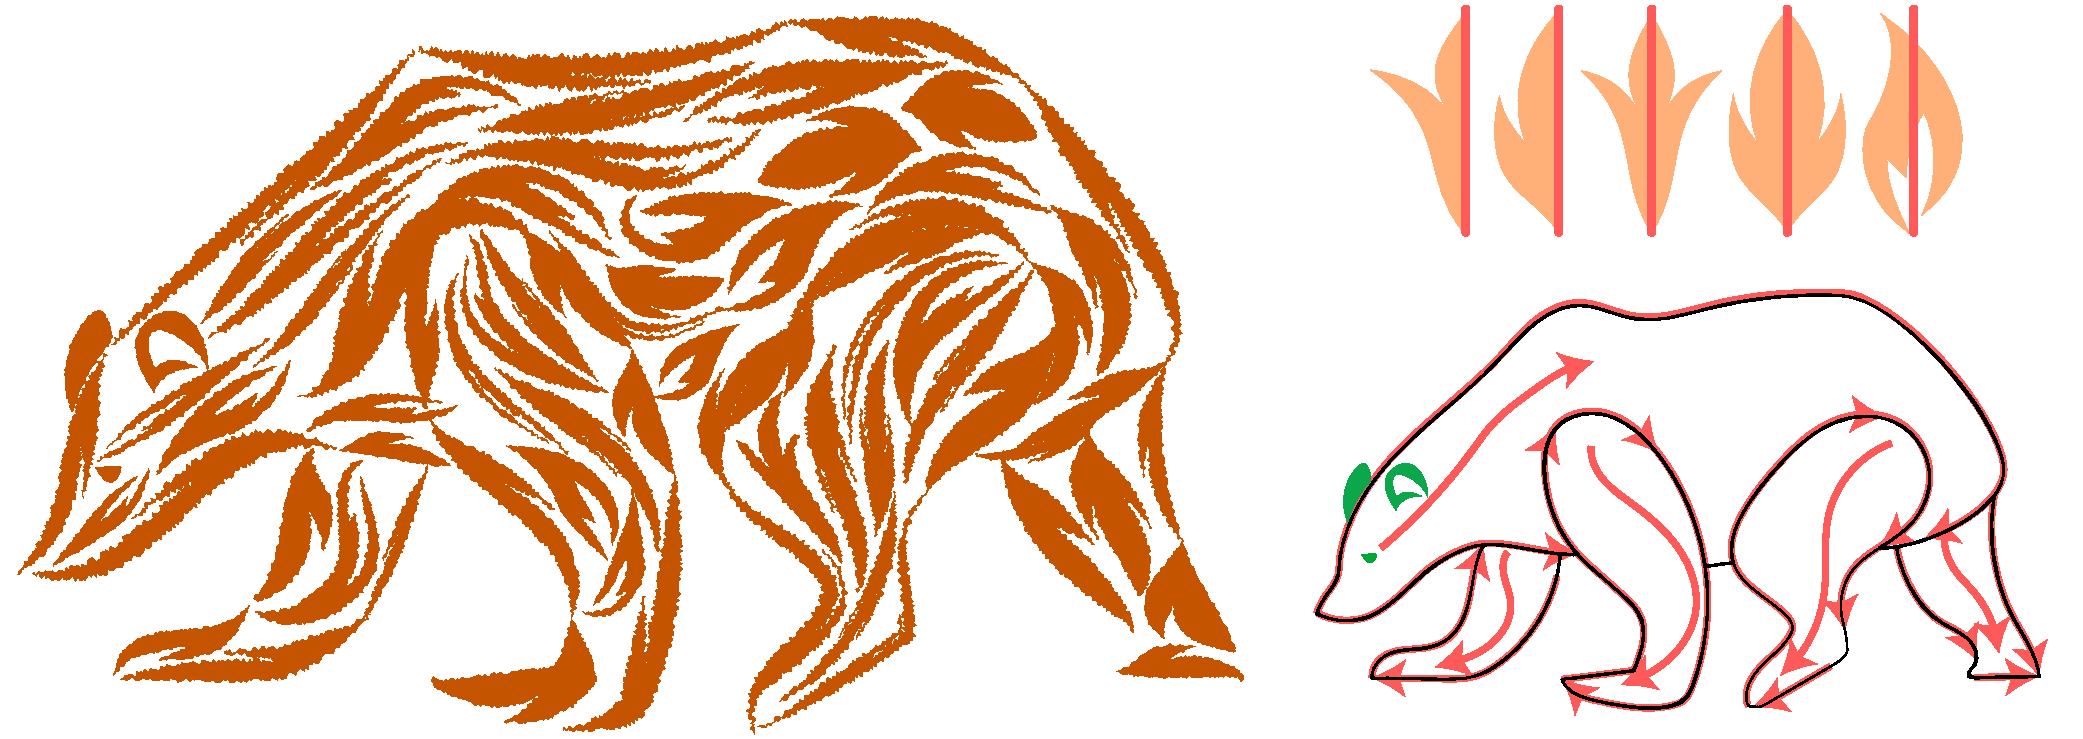
\includegraphics[width=1.0\textwidth]{figures/flowpak/bear_leaves.pdf} %BEAR LEAVES
\caption[A packing of a bear with leaf elements]
{\label{result_bear_leaves}
  A bear packing with leaf elements.  We manually add noise to the 
  elements in the output to create a distressed look.}
\end{figure}

%FFFFFFFFFFFFFFFFFFFFFFFFFFFFFFFFFFFFFFFFFFFFF
\begin{figure}
\centering

\includegraphics[width=1.0\textwidth]{figures/flowpak/cat.pdf}
\caption[A packing of a cat]
{A packing with a symmetric layout; we only compute the left half and reflect the result. The elements around the cheeks and the chin are not aligned to the boundary, creating a fur-like effect.}
\label{result_cat}
\end{figure}

%FFFFFFFFFFFFFFFFFFFFFFFFFFFFFFFFFFFFFFFFFFFFF
\begin{figure}
\centering
\vspace{-20pt}
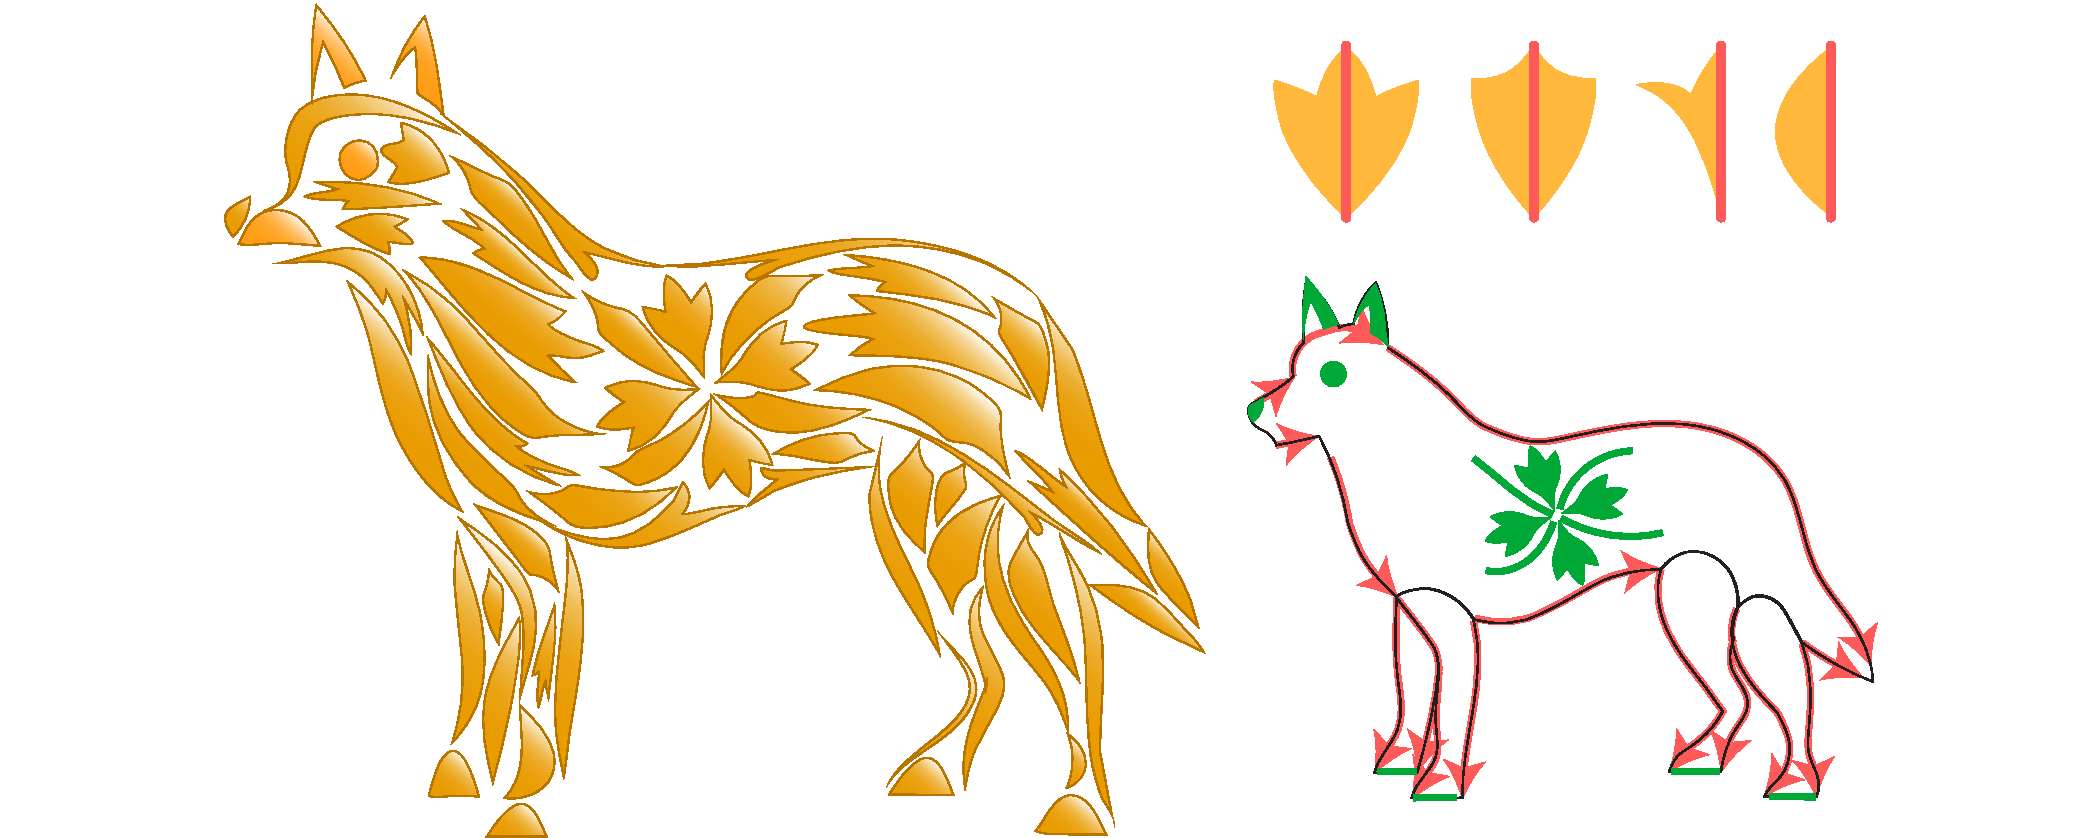
\includegraphics[width=1.0\textwidth]{figures/flowpak/dog_flower.pdf}
\caption[A packing of a dog]
{A packing of a dog. The fixed elements, shown as green
  shapes in the diagram, are copied as-is to the output; fixed spines,
  shown as green paths, force the placement of new elements at the given
  locations.}
\label{result_dog}
\end{figure}

%FFFFFFFFFFFFFFFFFFFFFFFFFFFFFFFFFFFFFFFFFFFFF
\begin{figure}
\centering
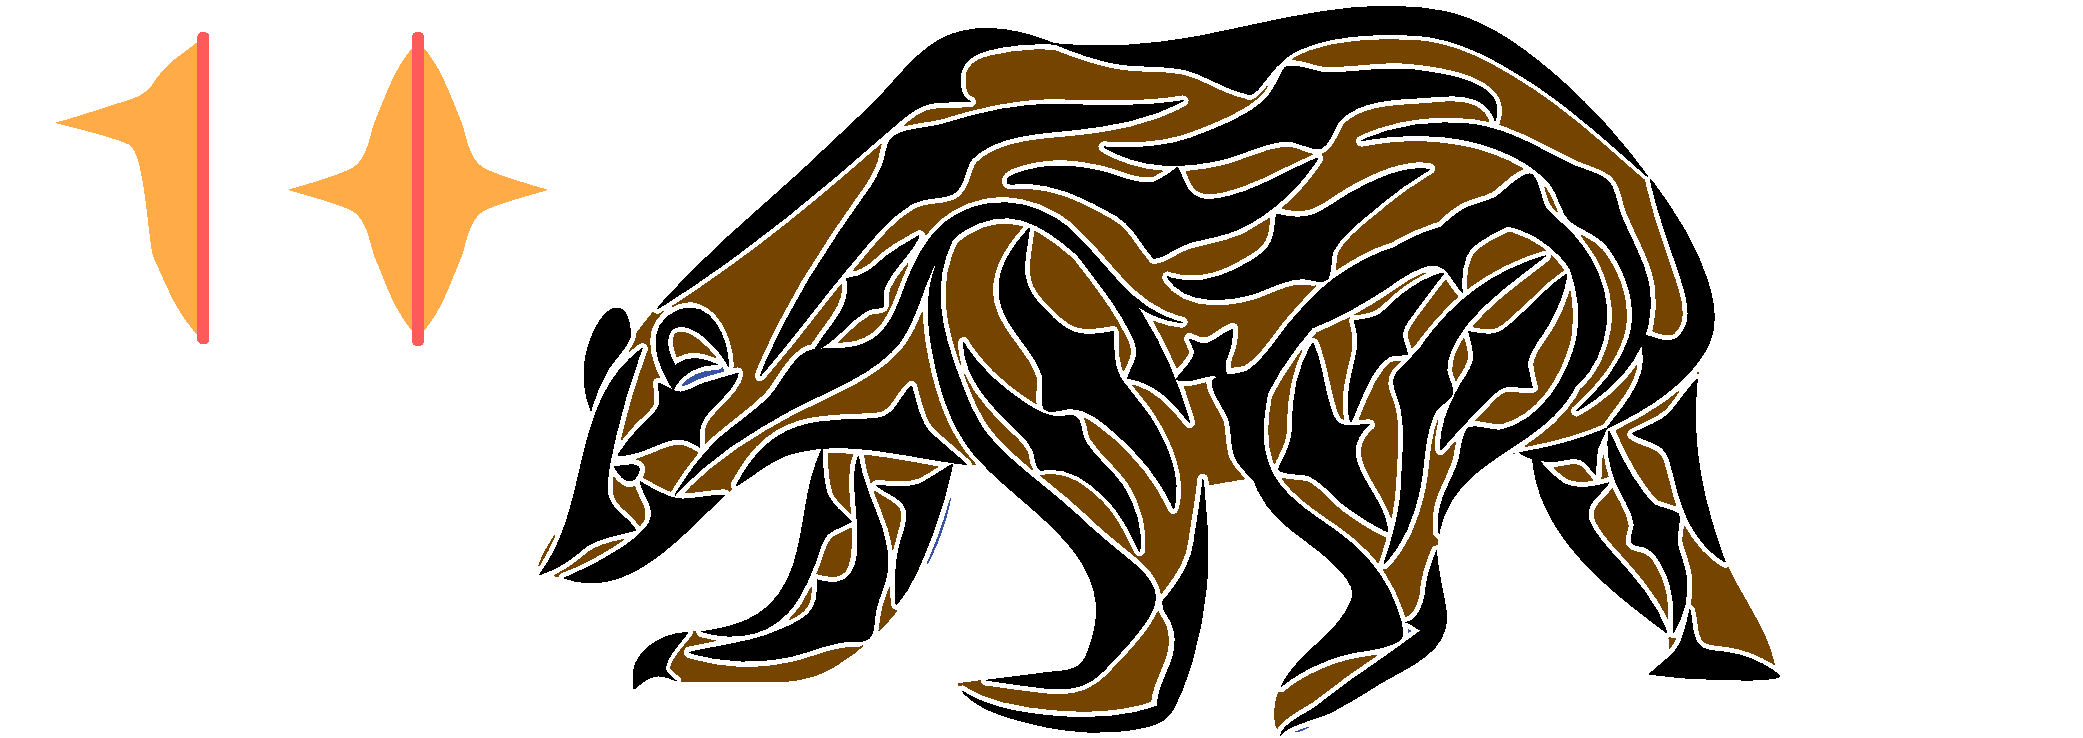
\includegraphics[width=1.0\textwidth]{figures/flowpak/bear_offset_space.pdf}
\caption[A packing of a bear with a few elements created from negative space]
{A packing of the same container as in Figure~\ref{result_bear_leaves}.
  We place longer and sparser elements and synthesize additional elements 
  from the remaining negative space.
  \newtext{The bottom row is the visualization of primary elements in black and
  negative space elements in brown.}
  }
\label{result_bear_offset}
\end{figure}

%FFFFFFFFFFFFFFFFFFFFFFFFFFFFFFFFFFFFFFFFFFFFF
\makeatletter % bruh
\setlength{\@fptop}{0pt} % bruh
\makeatother % bruh
\begin{figure}
\centering
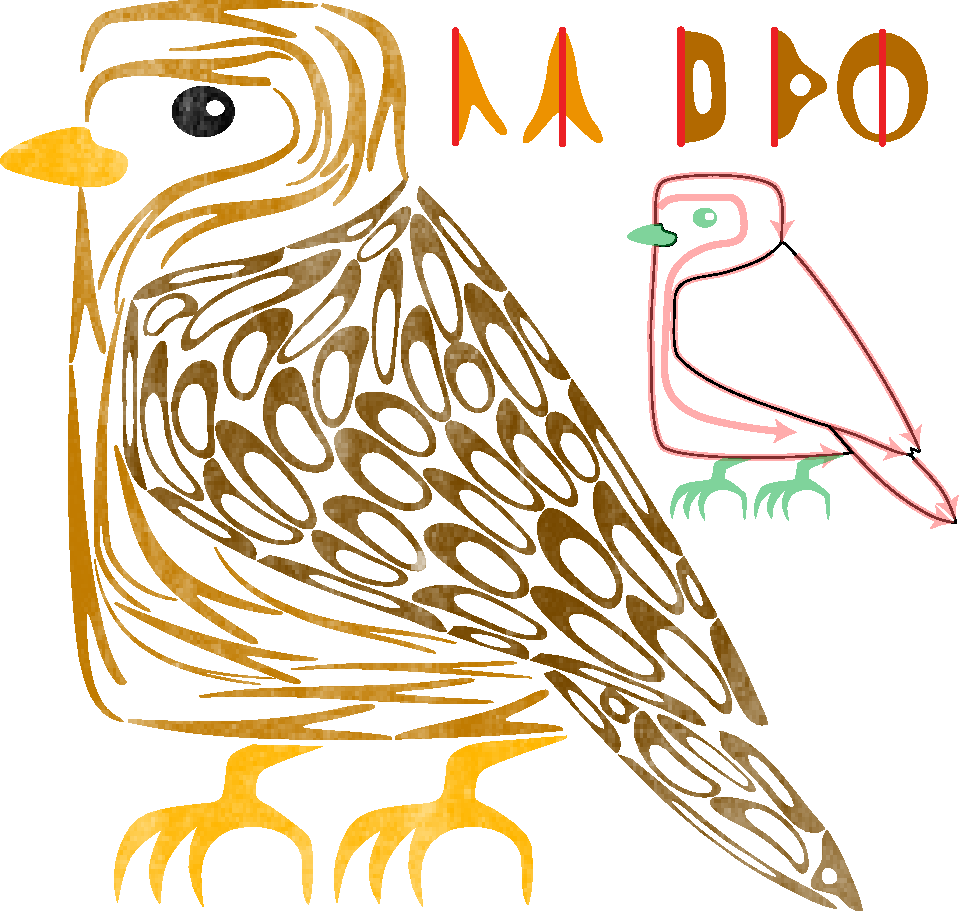
\includegraphics[width=1.0\textwidth]{figures/flowpak/bird_square.pdf}
\caption[A packing of a bird]
{A packing of a bird, based on input provided by
  an artist.}
\label{bird_square}
\end{figure}

\newcommand{\simforce}[1]{\bm{F}_{\kern -0.02in #1}}

%%%%%%%%%%%%%%%%%%%%%%%%%%%%%%%%%%%%%%%%%%%%%%%%%%%%%%%%%%
%%%%%%%%%%%%%%%%%%%%%%%%%%%%%%%%%%%%%%%%%%%%%%%%%%%%%%%%%%
\chapter[RepulsionPak: Deformation-Driven Element Packing \newline with Repulsion Forces]
{RepulsionPak: Deformation-Driven Element Packing with Repulsion Forces}
\label{chapter_repulsionpak}
%%%%%%%%%%%%%%%%%%%%%%%%%%%%%%%%%%%%%%%%%%%%%%%%%%%%%%%%%%
%%%%%%%%%%%%%%%%%%%%%%%%%%%%%%%%%%%%%%%%%%%%%%%%%%%%%%%%%%

\mynote{check if all points and vectors are bold}

\begin{figure*}[h!]
  \centering
  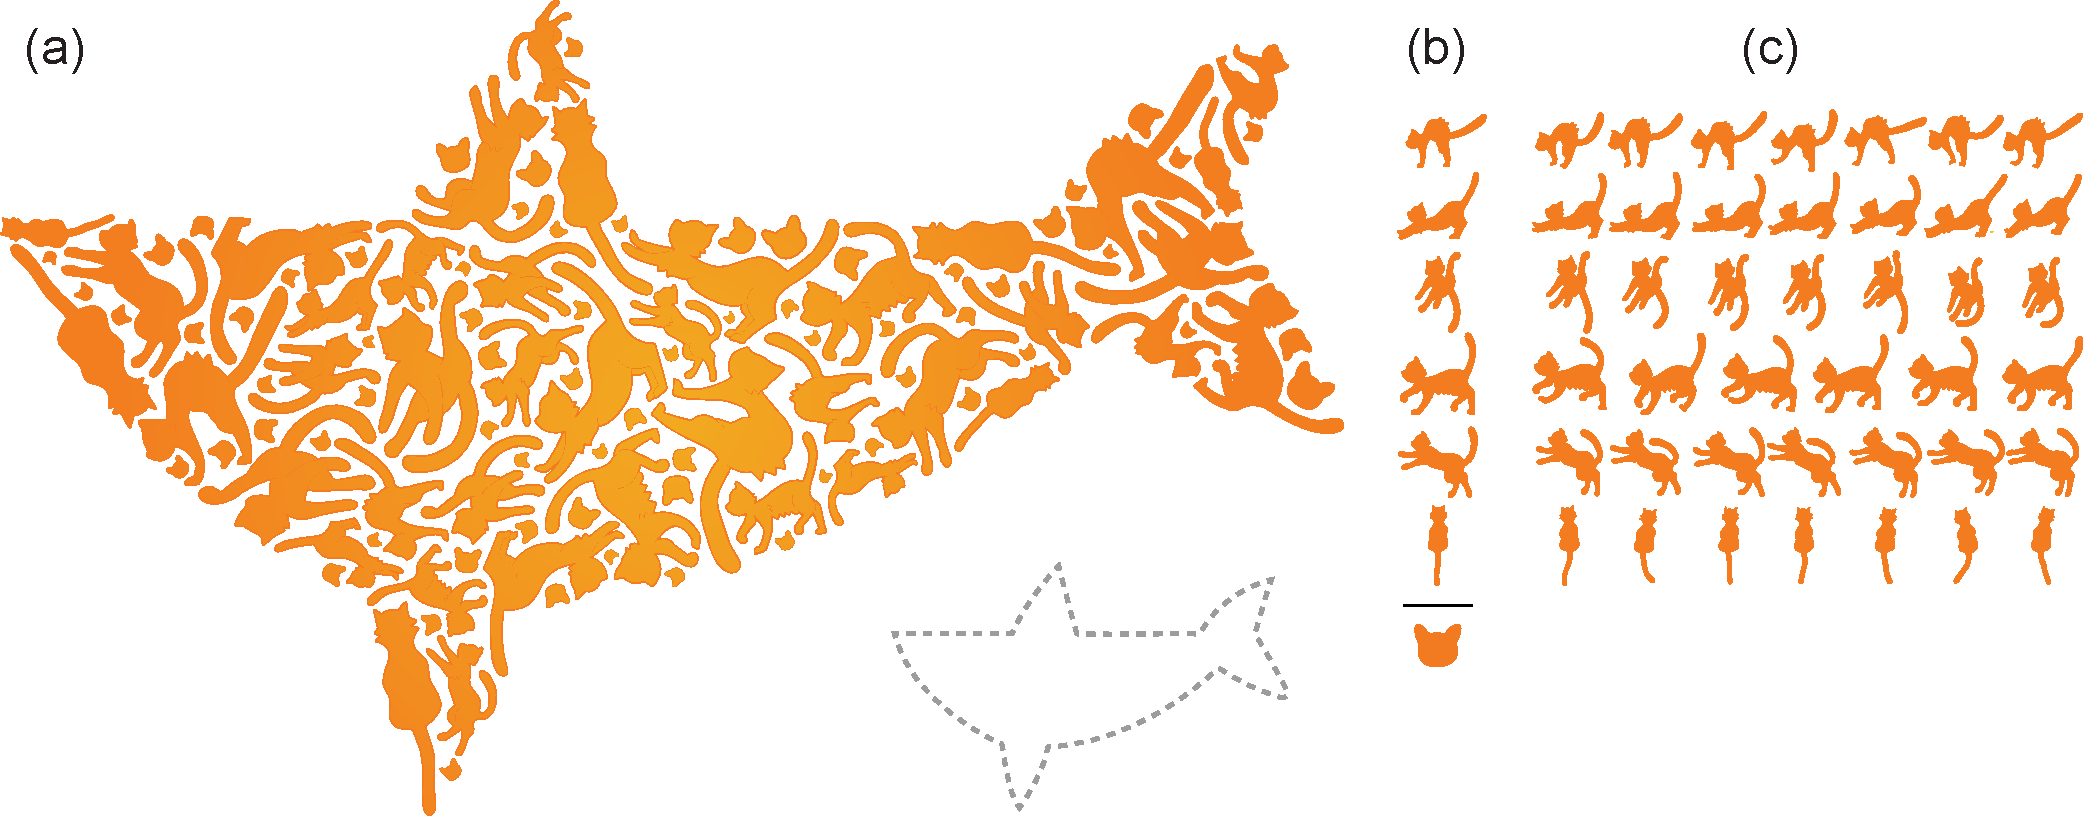
\includegraphics[width=1.0\textwidth]{figures/repulsionpak/cat_whale_04}
  \caption[A packing of a cat]
  {
  \label{cat_packing}
           A packing of six cat elements inside a fish-shaped target container. 
           Controllable deformation and repulsion forces allow the elements to deform,
           efficiently filling the container and creating a uniform distribution of
           negative space. We then reduce the remaining negative space by placing smaller
           cat heads. The gradient fill was added as a post-process.}
\end{figure*}



%%%%%%%%%%%%%%%%%%%%%%%%%%%%%%%%%%%%%%%%%%%%%%%%%%%%%%%%%%
%%%%%%%%%%%%%%%%%%%%%%%%%%%%%%%%%%%%%%%%%%%%%%%%%%%%%%%%%%
\section{Introduction}
\label{repulsionpak_introduction}
%%%%%%%%%%%%%%%%%%%%%%%%%%%%%%%%%%%%%%%%%%%%%%%%%%%%%%%%%%
%%%%%%%%%%%%%%%%%%%%%%%%%%%%%%%%%%%%%%%%%%%%%%%%%%%%%%%%%%



%%%%%%%%%%%%%%%%%%%%%%%%%%%%%%%%%%%%%%%%%%%%%%%%%%%%%%%%%%
%%%%%%%%%%%%%%%%%%%%%%%%%%%%%%%%%%%%%%%%%%%%%%%%%%%%%%%%%%
\section{Previous Work}
\label{repulsionpak_previous_work}
%%%%%%%%%%%%%%%%%%%%%%%%%%%%%%%%%%%%%%%%%%%%%%%%%%%%%%%%%%
%%%%%%%%%%%%%%%%%%%%%%%%%%%%%%%%%%%%%%%%%%%%%%%%%%%%%%%%%%

\mynote{Only talk about packings with deformation}


%%%%%%%%%%%%%%%%%%%%%%%%%%%%%%%%%%%%%%%%%%%%%%%%%%%%%%%%%%
%%%%%%%%%%%%%%%%%%%%%%%%%%%%%%%%%%%%%%%%%%%%%%%%%%%%%%%%%%
\section{System Overview}
\label{repulsionpak_system_overview}
%%%%%%%%%%%%%%%%%%%%%%%%%%%%%%%%%%%%%%%%%%%%%%%%%%%%%%%%%%
%%%%%%%%%%%%%%%%%%%%%%%%%%%%%%%%%%%%%%%%%%%%%%%%%%%%%%%%%%




\begin{figure}[h]
\centering
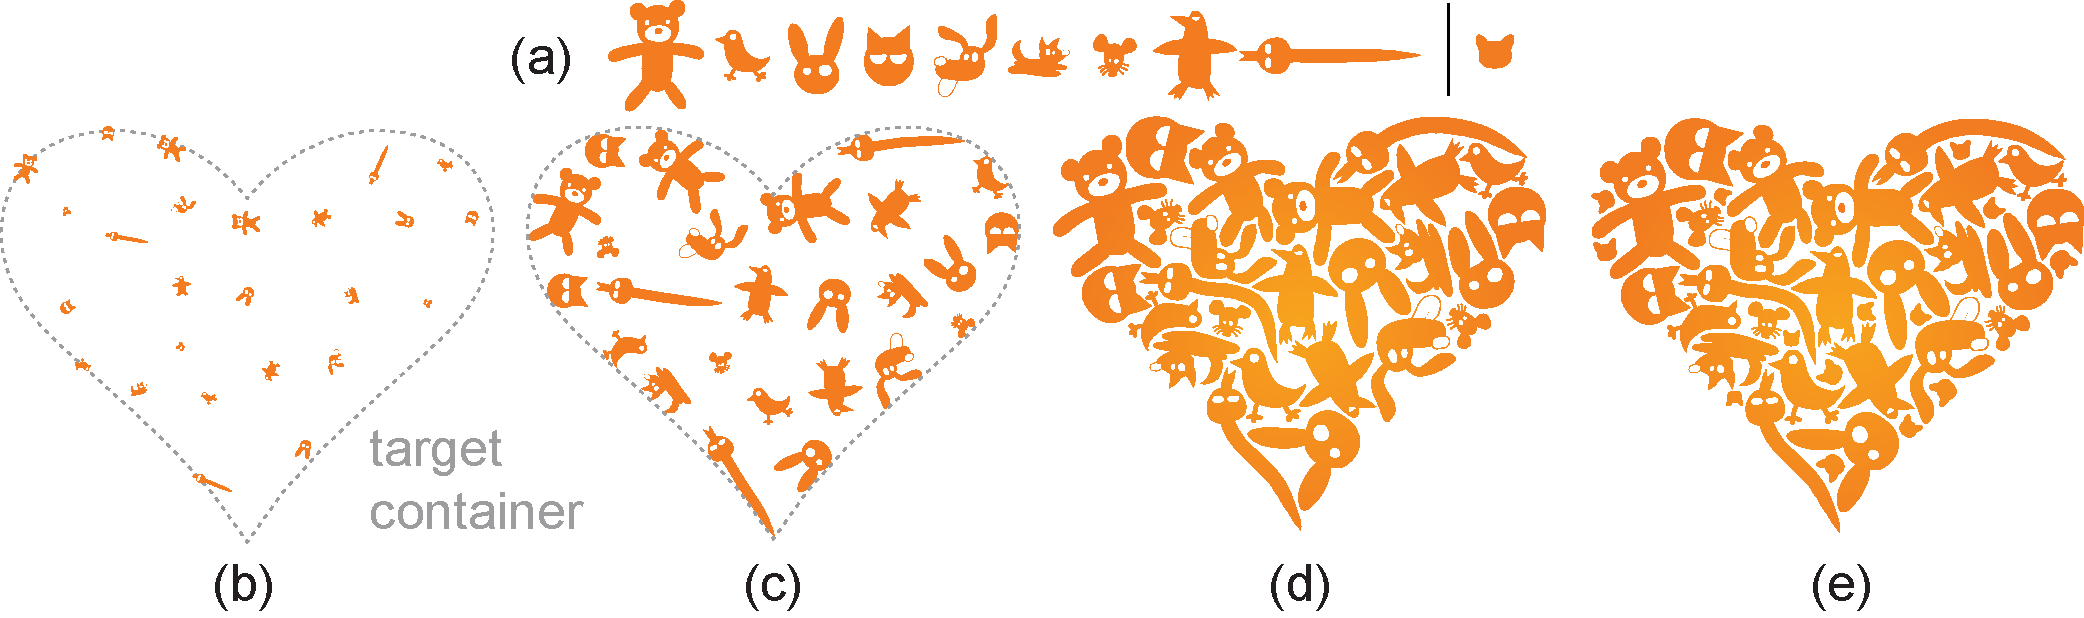
\includegraphics[width=1.0\textwidth]{figures/repulsionpak/pipeline.pdf} 
\caption[RepulsionPak pipeline]
{\label{fig_repulsionpak_pipeline} 
The creation of a packing using RepulsionPak.
  (a) A library of elements, comprising nine primary elements and a single
  	secondary element.
  (b) A target container with the initial distribution of scaled-down elements.
  (c) The simulation in progress, showing the elements growing, translating,
  	rotating, and deforming.
  (d) The resulting packing of primary elements.
  (e) The final result, after adding secondary elements and allowing them to
  	grow.
  	Fig.~\ref{fig_defviz} shows the deformations of some of the elements. }
\end{figure}

\begin{figure}[h]
\centering

\includegraphics[width=5cm]{figures/repulsionpak/pipeline_defviz_csk.pdf}
\caption[Element deformation]{
	\label{fig_defviz}
	Some of the elements in the final packing in Fig.~\ref{fig_repulsionpak_pipeline}, 
	showing the effect of deformation in our simulation.
}
\end{figure}

Our system requires three main pieces of input:
\begin{itemize}
	\item A library of primary and optional secondary elements, such
		as those shown in Fig.~\ref{fig_repulsionpak_pipeline}a.
	      Each element is a collection of 
		  open or closed polygonal paths---any curves must
		  be flattened ahead of time.
	\item One or more closed polygonal target containers, such as the
		heart in Fig.~\ref{fig_repulsionpak_pipeline}b.  Target containers can optionally
		have internal holes.
	\item The desired element spacing distance $d_\mathrm{gap}>0$.
\end{itemize}

RepulsionPak starts by preprocessing the elements, creating additional space around
each to enforce the spacing distance, and fitting a triangle mesh over each element.
\newtext{The containers are then seeded with randomly placed
copies of scaled-down elements 
(Section~\ref{repulsionpak_preprocessing}).}

\newtext{RepulsionPak} then performs a physics simulation on the meshes, 
making them simultaneously grow and repel each other. As a
proof of concept, we implement a spring-based 
simulation, \newtext{which yields satisfactory results despite its simplicity};
many alternatives are possible 
(see Section~\ref{repulsionpak_conclusions}).
Forces in the
simulation push mesh vertices away from vertices in other meshes,
attempt to keep the meshes from undergoing excessive deformation, and resolve
places where meshes overlap or vertices move outside target containers
(Section~\ref{repulsionpak_simulation}).

After each iteration of the simulation, meshes grow into adjacent space
if possible, so that they gradually consume the negative space in the container.
At the same time, mesh self-intersections are resolved
(Sections~\ref{repulsionpak_element_growth} and \ref{section_self_intersection_constraint}).
\mynote{delete self intersection section...}

The simulation concludes 
either when the elements occupy a sufficient proportion of the container area, or 
when some number of simulation steps fail to
significantly reduce the negative space
(Section~\ref{repulsionpak_stopping_criteria}).

Finally, an optional second simulation further reduces and evens out the
negative space.  It begins by placing small secondary elements in large
pockets of negative space.  This simulation is the same as the
first, except that vertices of primary element meshes are not allowed to move
(Section~\ref{repulsionpak_secondary_elements}).

Final SVG output is created by using barycentric coordinates to map each element's
paths from the element's initial mesh into the deformed mesh produced through
simulation.


%%%%%%%%%%%%%%%%%%%%%%%%%%%%%%%%%%%%%%%%%%%%%%%%%%%%%%%%%%
%%%%%%%%%%%%%%%%%%%%%%%%%%%%%%%%%%%%%%%%%%%%%%%%%%%%%%%%%%
\section{Preprocessing}
\label{repulsionpak_preprocessing}
%%%%%%%%%%%%%%%%%%%%%%%%%%%%%%%%%%%%%%%%%%%%%%%%%%%%%%%%%%
%%%%%%%%%%%%%%%%%%%%%%%%%%%%%%%%%%%%%%%%%%%%%%%%%%%%%%%%%%

\begin{figure}[t] %%% ELEMENT IMAGE
\centering
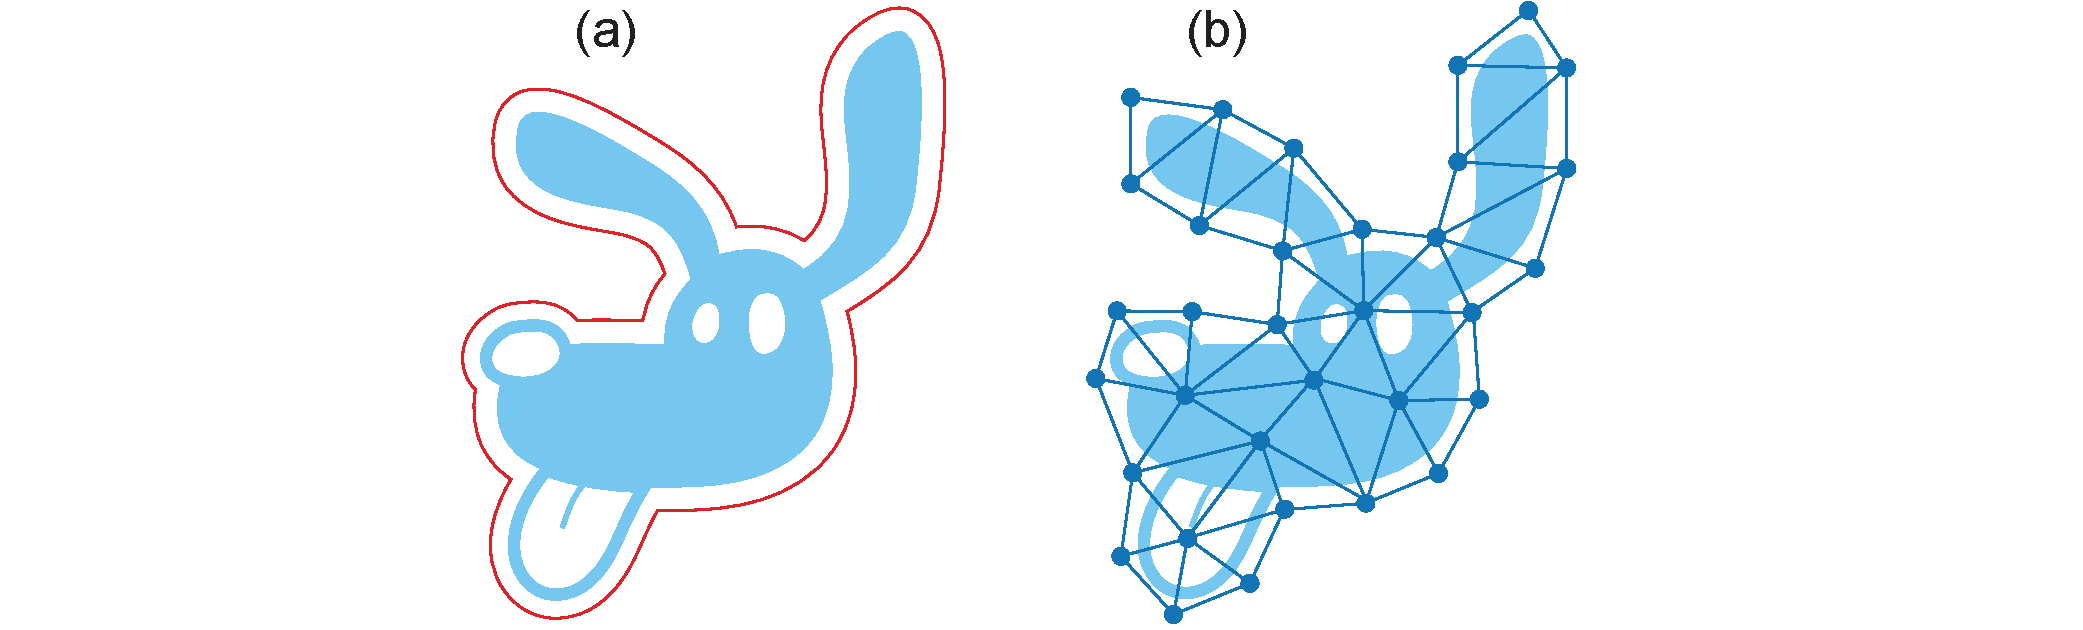
\includegraphics[width=4.5cm]{figures/repulsionpak/element_skin_triangles_2.pdf}
\caption[Element discretization]{
	\label{fig_elements_image}
	\newtext{An illustration of element discretization for preprocessing.}
	(a) An element with its boundary displaced to create a skin, drawn in red.
	(b) A triangle mesh with boundary vertices on the skin.
}
\end{figure}

\begin{figure*}[t]
\centering
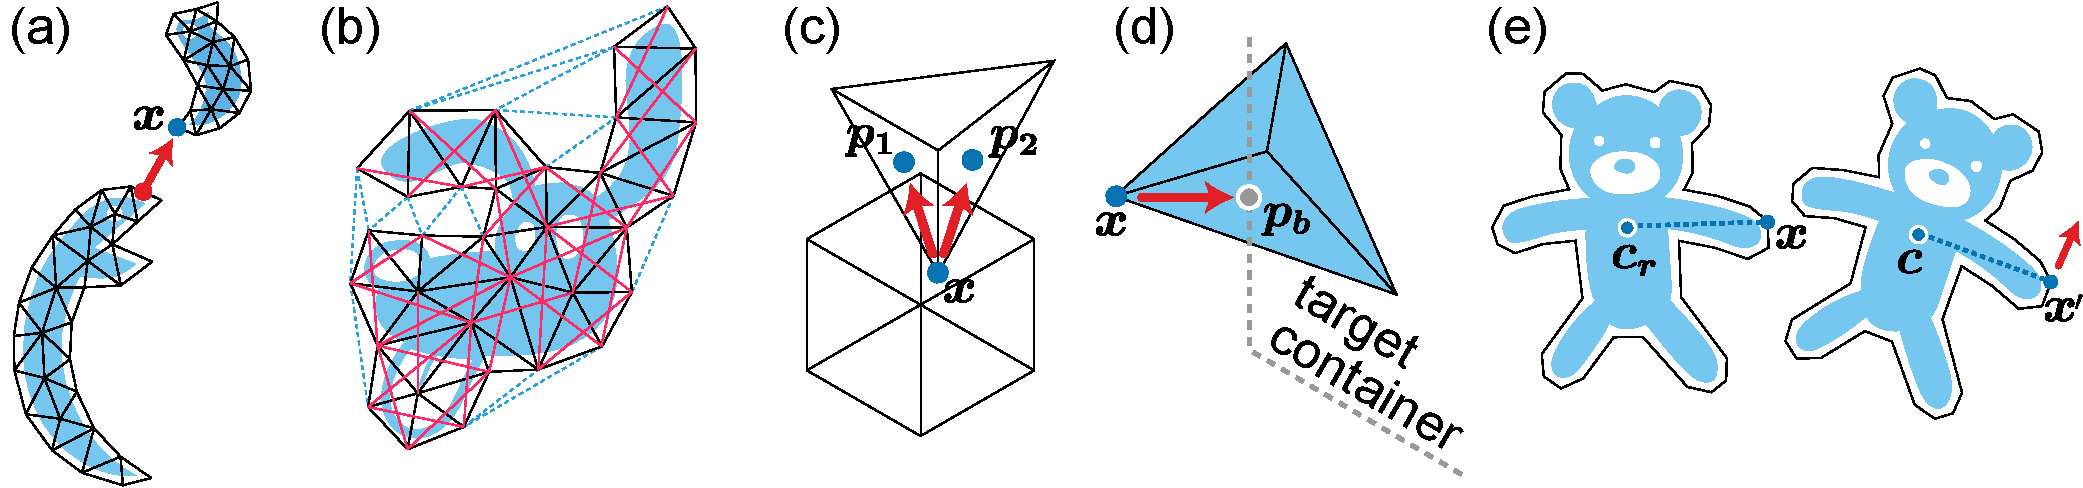
\includegraphics[width=1.0\textwidth]{figures/repulsionpak/all_forces_new.pdf}
\caption[Forces]{
\label{fig_forces}
Illustrations of the forces in our simulation.
\;\textbf{(a)~Repulsion force}:
The closest point on the snake's mesh
repels a vertex $\bm{x}$ in the bird mesh.
\textbf{(b)~Edge force}: 
We generate edge forces using
\newtext{edge springs (black), shear springs (red), and negative-space springs (dashed blue).}
\textbf{(c)~Overlap force}: 
Centres of triangles $\bm{p_1}$ and $\bm{p_2}$ attract a vertex
$\bm{x}$ that lies in the interior of another mesh.
\;\textbf{(d)~Boundary force}: A vertex $\bm{x}$ moves toward $\bm{p_b}$,
the closest point on a target container, when it is outside the container.
\textbf{(e)~Torsional force}: We restrict the orientation of the element by generating 
a torsional force at every boundary vertex $\bm{x}$
to restore its angular position relative to $\bm{c}$, 
the center of mass of the element.
\mynote
{
$\bm{c_r}$
points should be bold.
Should explain negative space edges, and shear edges.
}
}
\end{figure*}


The \textit{skin} of an element is a simple closed polygon 
that fully encloses it, 
as in the red shape in Figure~\ref{fig_elements_image}(a).
We generate the skin 
by offsetting 
an element's boundary outward by $d_\mathrm{gap}/2$. 
The simulation aims to produce an approximate tessellation of the target
container by \newtext{deformed} skins, thereby achieving the desired element spacing and
suppressing overlaps.

We triangulate the element skin to obtain a triangle mesh.
To create the mesh we uniformly sample the skin polygon $s$, with samples
spaced apart by distance $d_\mathrm{gap}$,
to obtain a simpler polygon $s'$ (the outer boundary of the mesh).
We then construct a Delaunay triangulation of $s'$.
The vertices and edges of this mesh become unit 
masses and longitudinal
springs in a physical simulation, allowing elements to deform in response to
their neighbours.  
We further brace the mesh against
deformation by augmenting it with ``auxiliary springs'' (see
Section~\ref{section_forces} and Fig.~\ref{fig_forces}b).

Due to discretization, a low mesh resolution does not guarantee a separation of $d_\mathrm{gap}$. 
Increasing the mesh resolution produces a more precise result at the expense of greater running time.

\textbf{Barycentric coordinates:}
The simulation operates on meshes, not element geometry.  In the final
rendering phase, we will redraw an element relative to a deformed copy of
its mesh.  To do so, we first re-express every vertex of an element path in 
terms of the mesh triangles.  Every element vertex lies either inside a mesh
triangle or just beyond a border edge.  We encode each vertex in barycentric
coordinates relative to its enclosing or nearest triangle.

\textbf{Initial element placement:}
We prepare our simulation by randomly placing non-overlapping elements.
\begin{enumerate}
	\item Generate random points $P = \{ p_1, p_2,..., p_n \}$ 
		  inside the target container 
	      via blue noise sampling~\cite{Bridson2007}.
	      The user controls the number of points; using more points gives results
	      with smaller elements.  We can automatically estimate $n$ by
		  dividing the container area by the desired average area of the element skins.
	\item Cycle through the primary elements, assigning each element to a 
		  random unused $p_i$ with a random orientation, repeating until 
		  every point has an element.
	\item Shrink all the elements so that they do not overlap and occupy only
		  a small fraction of the container's area; in our implementation we
		  have found that $5-10$\% of the area gives good results. Making them
		  larger would speed up the simulation but does
	      not allow enough freedom of movement to generate successful
		  packings.  Fig.~\ref{pipeline}b shows an initial placement.	      
\end{enumerate}


%%%%%%%%%%%%%%%%%%%%%%%%%%%%%%%%%%%%%%%%%%%%%%%%%%%%%%%%%%
%%%%%%%%%%%%%%%%%%%%%%%%%%%%%%%%%%%%%%%%%%%%%%%%%%%%%%%%%%
\section{Simulation}
\label{repulsionpak_simulation}
%%%%%%%%%%%%%%%%%%%%%%%%%%%%%%%%%%%%%%%%%%%%%%%%%%%%%%%%%%
%%%%%%%%%%%%%%%%%%%%%%%%%%%%%%%%%%%%%%%%%%%%%%%%%%%%%%%%%%

We design a simulation in which 
we generate pseudo-physical 
forces that transform elements by transforming their meshes.
Let $\bm{x}$ be a vertex of an element mesh. 
The total force $\bm{F}$ applied to $\bm{x}$ is
\begin{equation}
\bm{F} = \simforce{r} + \simforce{e} + \simforce{b} + \simforce{o} + \simforce{t}
\end{equation}
where $\simforce{r}$, $\simforce{e}$, $\simforce{b}$, $\simforce{o}$ and $\simforce{t}$ are 
the repulsion force, the edge force, the boundary force, the overlap force, \newtext{and the torsional force}.
These forces combine with the growth process, described in
Section~\ref{section_growing_element}, to completely fill the target container.

%%%%%%%%%%%%%%%%%%%%%%%%%%%%%%%%%%%%%%%%%%%%%%%%%%%%%%%%%
%%%%%%%%%%%%%%%%%%%% REPULSION FORCE %%%%%%%%%%%%%%%%%%%%
%%%%%%%%%%%%%%%%%%%%%%%%%%%%%%%%%%%%%%%%%%%%%%%%%%%%%%%%%

%% CSK TODO: what counts as a "nearest neighbouring mesh" in this context?
%% How do we know which neighbours to iterate over?

\medskip
\textbf{Repulsion force:} 
The repulsion force tries to push element meshes apart when they approach
each other, with the goal of
making them transform to align their boundaries (Fig.~\ref{fig_forces}a).
 
The vertex $\bm{x}$ will
experience an inverse square repulsive force, inspired by Coulomb's law,
from all nearby meshes.  We use the following formula:

\begin{equation}
\simforce{r} = k_r \sum_{i = 1}^{n} \frac{\bm{u}}{\| \bm{u} \| }\frac{1}{\varsigma  +\| \bm{u} \|^2 }
\end{equation}
where 
\begin{packeddescriptions}
	\item[$k_r$]        is the strength of the repulsion force relative to
						other forces in the simulation.
	\item[$n$]        is the number of nearest neighbouring meshes to $\bm{x}$. 
	\item[$\bm{x_{i}}$] is the closest point on the skin of the $i$th neighbour.
	\item[$\bm{u}$]  $= \bm{x} - \bm{x_{i}}$
	
						% mesh from $\bm{x}$.		
	
	\item[$\varsigma$]   is a \textit{soft parameter}; it places an upper 
						bound on the magnitude of $\simforce{r}$, avoiding
						explosive instability when $\| \bm{u} \|$ is very small.
\end{packeddescriptions}

An imbalance in the repulsion forces across a mesh's vertices will
naturally induce translation and rotation in meshes, helping their
boundaries discover compatible segments and consuming more of the
remaining negative space.

If $\bm{x}$ lies inside of another element's mesh, then the aggregate repulsion
force from other neighbours can push $\bm{x}$ further inside and
worsen the overlap.  If we discover such an overlap, we set
$\simforce{r}$ to $0$ and use the overlap force $\simforce{o}$, discussed below, to
correct it.

%%%%%%%%%%%%%%%%%%%%%%%%%%%%%%%%%%%%%%%%%%%%%%%%%%%%
%%%%%%%%%%%%%%%%%%%% EDGE FORCE %%%%%%%%%%%%%%%%%%%%
%%%%%%%%%%%%%%%%%%%%%%%%%%%%%%%%%%%%%%%%%%%%%%%%%%%%
\medskip
\textbf{Edge force:} 
%\deadtext{By converting element meshes into mass-spring systems,
%we allow elements to undergo deformation in response to repulsion forces
%exerted by neighbours.  A mesh's edges become longitudinal \textit{edge springs}.}
A mesh's edges are treated as longitudinal \textit{edge springs};
displacement
of these springs allows a mesh to deform in response to repulsion forces
by neighbouring meshes.
In addition, when two mesh triangles share an edge we connect the two vertices
opposite the edge with an \textit{auxiliary spring} (Fig.~\ref{fig_forces}b), 
adding extra bracing to a mesh to prevent it from folding.

An undeformed element mesh provides the rest lengths for all of
its springs; as mesh vertices move relative to each other, the springs
attempt to restore these rest lengths.  Let $\bm{x_{a}}$ and $\bm{x_{b}}$ be
mesh vertices connected by a spring.  We compute the spring force as follows:
% As we apply forces to the masses, springs get shorter or longer, causing
% the element to deform. The edge forces attempt to restore the springs
% back to their rest lengths. 
% If a pair of masses $\bm{x_a}$ and $\bm{x_b}$ are connected by a spring,
% the edge force $\simforce{e}$ is applied to to the mass $\bm{x_a}$, 
% and $-\simforce{e}$ is applied to to the mass $\bm{x_b}$:

\begin{equation}
\simforce{e} =  k_{e} \frac{\bm{u}}{\| \bm{u} \|} s \; ( \| \bm{u} \| - \ell)^2
\end{equation}
where
\begin{packeddescriptions}
	\item[$k_e$] is the strength of the edge force relative to other forces.
	\item[$\bm{u}$] $= \bm{x_{b}} - \bm{x_{a}}$
	\item[$\ell$] is the rest length of the spring.
	\item[$s$] is +1 or -1, according to whether $(\| \bm{u} \| - \ell)$ 
		is positive or negative.
\end{packeddescriptions}

We apply $\simforce{e}$ to $\bm{x_{a}}$ and $-\simforce{e}$ to $\bm{x_{b}}$.
The equation is a modification of Hooke's law
in which the strength of the force increases quadratically
with displacement.
This change allows the meshes to resist severe deformations
when subjected to powerful forces.

% \paul{Also needed: Why two kinds of springs?  Why are edge springs not enough?
% Why do you call it a bending spring?}

%%%%%%%%%%%%%%%%%%%%%%%%%%%%%%%%%%%%%%%%%%%%%%%%%%%%%%%
%%%%%%%%%%%%%%%%%%%% OVERLAP FORCE %%%%%%%%%%%%%%%%%%%%
%%%%%%%%%%%%%%%%%%%%%%%%%%%%%%%%%%%%%%%%%%%%%%%%%%%%%%%

%% CSK TODO: verify that "centroid" is the right word here.

\medskip
\textbf{Overlap force:}
Occasionally, a vertex $\bm{x}$ from one mesh can be pushed inside the skin of a
neighbouring mesh.  In such cases, we temporarily disable the repulsion force
on this vertex
by setting it to 0, and instead apply an overlap force that attempts to
eject the intruding vertex.  In particular, every mesh triangle having $\bm{x}$
as a vertex will pull $\bm{x}$ in the direction of its centroid.  The overlap
force is thus given by:

\begin{equation}
\simforce{o} = k_o \sum_{i = 1}^{n} (\bm{p_{i}} - \bm{x})
\end{equation}
where
\begin{packeddescriptions}
	\item[$k_o$] is the relative strength of the overlap force.
	\item[$n$] is the number of mesh triangles that have $\bm{x}$ as a vertex.
	\item[$\bm{p_{i}}$] is the centroid of the $i$th triangle incident on $\bm{x}$.
\end{packeddescriptions}

The overlap force is zero for vertices that are not within another mesh.

%%%%%%%%%%%%%%%%%%%%%%%%%%%%%%%%%%%%%%%%%%%%%%%%%%%%%%%%
%%%%%%%%%%%%%%%%%%%% BOUNDARY FORCE %%%%%%%%%%%%%%%%%%%%
%%%%%%%%%%%%%%%%%%%%%%%%%%%%%%%%%%%%%%%%%%%%%%%%%%%%%%%%
\medskip
\textbf{Boundary force:}
The boundary force causes element meshes to stay inside the target container
and conform to its boundary. It applies to any vertex $\bm{x}$ that
is outside the container, and moves the vertex towards the closest point
on the container's boundary, by an amount proportional to the distance to
the boundary:
%%% EQ
\begin{equation}
\simforce{b} = k_{b} (\bm{p_b} - \bm{x})
\end{equation}
where
\begin{packeddescriptions}
	\item[$k_b$] is the relative strength of the boundary force.
	\item[$\bm{p_b}$] is the closest point on the target container to $\bm{x}$.
\end{packeddescriptions}

The boundary force is zero for any point inside the container.

\medskip
\textbf{Torsional force:} 
\newtext{
As forces propagate through an element mesh, the aggregate velocity
vectors of the vertices can induce a rotation of the entire element.
However, some elements may have a preferred orientation,
either for aesthetic reasons or because the shape is comprehensible only at certain orientations.
We introduce a torsional force that
penalizes individual vertices for which the orientation, relative to their
element's center of mass, drifts too far from its initial orientation.
}

\newtext{
Consider a vertex $\bm{x}$ belonging
to an element, and let $\bm{c}_r$ be the element's center of mass in
its undeformed state.  We may define the ``rest orientation'' of
$\bm{x}$ as the orientation of the vector $\bm{u}_r = \bm{x}-\bm{c}_r$.
During simulation we compute the current centre of mass $\bm{c}$ of 
the element and let $\bm{u}=\bm{x}-\bm{c}$.  Then the torsional force
is
}
\newtext{
\begin{equation}
  \simforce{t} =\begin{cases}
    k_t\bm{u}^\perp, & \theta > 0\\
    -k_t\bm{u}^\perp, & \theta < 0
  \end{cases}
\end{equation}
where
\begin{packeddescriptions}
	\item[$k_t$]  is the relative strength of the torsional force.
	\item[$\theta$] is the signed angle between $\bm{u}_r$ and $\bm{u}$;
	\item[$\bm{u}^\perp$] is a unit vector rotated $90^\circ$
		counterclockwise relative to $\bm{u}$; and
\end{packeddescriptions}
}
\newtext{
Using the equation above, $\simforce{t}$ is always perpendicular to $\bm{u}$
and the direction of $\simforce{t}$ points to the left or to the right depending on $\theta$.
Unlike the first four force types, the torsional force is optional.}

%%%%%%%%%%%%%%%%%%%%%%%%%%%%%%%%%%%%%%%%%%%%%%%%%%%%%%%
%%%%%%%%%%%%%%%%%%%% THE SIMULATION %%%%%%%%%%%%%%%%%%%
%%%%%%%%%%%%%%%%%%%%%%%%%%%%%%%%%%%%%%%%%%%%%%%%%%%%%%%

\medskip
\textbf{Simulation details:} 
We use explicit Euler integration to simulate the motions of the mesh vertices under the
forces described above.  Every vertex has a position and a velocity vector; in
every iteration, we update velocities using forces, and update positions using
velocities.  These updates are scaled by a time step $\Delta t$, typically
chosen from the range $[0.01,0.1]$.  A smaller time step results in a more
stable simulation at the cost of additional running time.  We cap velocities
at $5\Delta t$ to dissipate extra energy from the system.

%% CSK TODO: verify these measurements.

The repulsion and overlap forces rely on nearest-neighbour queries on the
set of all vertices.  We accelerate these queries by storing vertices in a
uniform spatial subdivision grid that covers the container.  In our
implementation, cell width and height are $6-10$\% of the larger dimension
of the grid.  
%\deadtext{We identify the neighbours of a vertex $\bm{x}$ by considering}
We define the neighbours of a vertex $\bm{x}$ as
all vertices in a $3\times 3$ window of cells centred on the cell
containing $\bm{x}$. 
%\deadtext{Although this is an approximation, since it can miss 
%distant vertices in the composition, the effect is insignificant because of the
%low magnitude of forces involving these vertices.}
This approximation ignores the negligible interactions between
distant vertices.

The constants $k_r$, $k_o$, $k_b$  $k_e$, and $k_t$ control the relative strengths
of the five forces in the simulation.  They must also be chosen relative to
the time step $\Delta t$ and the overall width and height of the container.
We find that our simulation produces satisfactory results when 
$k_r \approx k_o \approx k_b \geq k_e > k_t$.
%\begin{equation}
%k_r \approx k_o \approx k_b \geq k_e
%\end{equation}
For example, if the container's bounding box is approximately $1000\times 1000$,
then we have obtained good results when $k_r=k_o=k_b=80$, $k_e=40$, and $k_t=1$.  We also
set $\varsigma=1$ to avoid explosive repulsion forces.  Increasing $k_e$
relative to the other forces suppresses deformation, yielding a close approximation
of packing with rigid elements.


%%%%%%%%%%%%%%%%%%%%%%%%%%%%%%%%%%%%%%%%%%%%%%%%%%%%%%%%%%
%%%%%%%%%%%%%%%%%%%%%%%%%%%%%%%%%%%%%%%%%%%%%%%%%%%%%%%%%%
\subsection{Element Growth}
\label{repulsionpak_element_growth}
%%%%%%%%%%%%%%%%%%%%%%%%%%%%%%%%%%%%%%%%%%%%%%%%%%%%%%%%%%
%%%%%%%%%%%%%%%%%%%%%%%%%%%%%%%%%%%%%%%%%%%%%%%%%%%%%%%%%%

RepulsionPak starts with small initial elements to avoid intersections,
and gradually enlarges them until they tightly fill the target
container.  Fig.~\ref{pipeline}c-d shows elements growing and gradually
consuming negative space.  Elements have different intrinsic sizes, which are
respected in the initial placement.  Because they all grow at roughly the
same rate, their relative sizes tend to be maintained.

After each iteration of the physics simulation, the element meshes undergo
a growth step.  If an element mesh has no vertices that lie inside of
neighbouring meshes, it is permitted to grow in this iteration.  A mesh with
overlaps may still grow in subsequent iterations, if local changes to the 
packing open up more negative space.
This approach produces \newtext{slight variations} in skin offsets in the output packing
but the effect \newtext{is negligible.}

We implement growth in the context of the physics simulation by scaling
the rest lengths of a mesh's springs, allowing it to expand as the simulation
progresses.  Every mesh $M$ has a counter $n_M$ that records the number of
times it has grown.  When a mesh is permitted
to grow, we add 1 to the counter.  Then, if $L_i$ is the rest length
of the $i$th spring in the original undeformed mesh, we increase its rest
length to $(1+n_Mk_g\Delta t)L_i$.  The constant $k_g$,
usually 0.01 in our system, controls the growth rate.


%%%%%%%%%%%%%%%%%%%%%%%%%%%%%%%%%%%%%%%%%%%%%%%%%%%%%%%%%%
%%%%%%%%%%%%%%%%%%%%%%%%%%%%%%%%%%%%%%%%%%%%%%%%%%%%%%%%%%
\subsection{Stopping Criteria}
\label{repulsionpak_stopping_criteria}
%%%%%%%%%%%%%%%%%%%%%%%%%%%%%%%%%%%%%%%%%%%%%%%%%%%%%%%%%%
%%%%%%%%%%%%%%%%%%%%%%%%%%%%%%%%%%%%%%%%%%%%%%%%%%%%%%%%%%


We choose one of two criteria to stop the simulation. First, the artist specifies 
the desired positive space ratio at which the simulation immediately terminates.
The ratio should not be set too high, and
we find that most packings have positive space ratios between $45\%$ and $65\%$ depending on the element shapes.
For example, concave elements with long extensions are more difficult to pack, 
so a lower positive space ratio is recommended to generate a satisfactory packing.
Second, we stop the simulation when the element meshes are no longer
able to maneuver enough to consume the remaining negative space. 
After each iteration, we compute an \textit{area fraction} $A$, defined to be the fraction of
the container area taken up by element meshes.  We then compute a measurement
of the recent change in area fraction in a sliding window that covers the $w$
most recent iterations of the system; we use $w=100$.  If $A_0,\ldots,A_w$
are the area fractions in the $w+1$ iterations up to the current one, then we
define

\begin{equation}
\mathrm{RMS} = \sqrt{ \frac{1}{w}\sum_{ i = 1 }^{w} { (A_i - A_{i-1}) }^2}
\end{equation}

We stop iterating when $\mathrm{RMS} < \epsilon$, where $\epsilon$ is $0.01$
in our system.

%%%%%%%%%%%%%%%%%%%%%%%%%%%%%%%%%%%%%%%%%%%%%%%%%%%%%%%%%%
%%%%%%%%%%%%%%%%%%%%%%%%%%%%%%%%%%%%%%%%%%%%%%%%%%%%%%%%%%
\section{Secondary Elements}
\label{repulsionpak_secondary_elements}
%%%%%%%%%%%%%%%%%%%%%%%%%%%%%%%%%%%%%%%%%%%%%%%%%%%%%%%%%%
%%%%%%%%%%%%%%%%%%%%%%%%%%%%%%%%%%%%%%%%%%%%%%%%%%%%%%%%%%

The iteration process described above can leave behind isolated pockets of 
empty space, which will be visible in the final composition.  We imitate the
approach taken by human artists by filling these pockets will small, usually
simple secondary elements.  

We seed the container with secondary elements by finding points
that are far from any existing element mesh.  Specifically, we
compute a discrete approximation of the distance transform of the
negative space. We then create an initial candidate list of all
points for which the distance value is above a threshold $d_\mathrm{min}$, sorted
by decreasing distance.  We consider each of these candidates in turn,
adding it to a final list of seed locations provided that no previously
chosen seed is within distance $d_\mathrm{sep}$ of the candidate.
In our implementation, if the distance transform is computed on a 
$1000\times 1000$ grid fit to the container's bounds, then we typically 
set $5 \leq d_\mathrm{min} \leq 10$ and $d_\mathrm{sep}=10$. 

Next, we assign random secondary elements to these chosen seed
points, scaled down as before to avoid overlaps.  We then run the
simulation and growth process again, but freeze the primary elements:
they exert repulsion forces on secondary elements and can induce
overlaps, but primary mesh vertices cannot move.  The secondary
elements gradually grow to consume some of the remaining negative
space until the packing satisfies the same stopping \newtext{criteria}
described above.

Packings with secondary elements are shown throughout the paper; 
see Figs.~\ref{pipeline}e, \ref{cat_packing}, and \ref{three_packings}.


%%%%%%%%%%%%%%%%%%%%%%%%%%%%%%%%%%%%%%%%%%%%%%%%%%%%%%%%%%
%%%%%%%%%%%%%%%%%%%%%%%%%%%%%%%%%%%%%%%%%%%%%%%%%%%%%%%%%%
\section{Shape Matching}
\label{repulsionpak_shape_matching}
%%%%%%%%%%%%%%%%%%%%%%%%%%%%%%%%%%%%%%%%%%%%%%%%%%%%%%%%%%
%%%%%%%%%%%%%%%%%%%%%%%%%%%%%%%%%%%%%%%%%%%%%%%%%%%%%%%%%%



\begin{figure}[t]
\centering

\includegraphics[width=0.3\columnwidth]{figures/repulsionpak/descriptor_2.pdf}
\caption[A local shape descriptor for shape matching]
{\label{fig_shape_matching}
\newtext{An illustration of a local shape descriptor with $n = 3$. 
These segments have varying arclengths but they all have the same value
of $\tau$, the integral of absolute curvature along their lengths.}
}
\end{figure}
\begin{figure}
\centering
\includegraphics[width=0.95\columnwidth]{figures/repulsionpak/rhino_shape_matching_bitmap.pdf} 
\caption[A demonstration of shape matching of leaf shapes inside a rhinoceros]
{\label{rhino_packing}
{ 
A demonstration of shape matching of leaf shapes inside a rhinoceros. 
(a) We detect nine salient features, namely sharp convex corners, and 
assign an element to each.
(b) A spring holds each element in place.
(c) The final result.
}
}
\end{figure}

The motions and deformations of elements, as described
in the previous sections, give them an opportunity to conform to each 
other and to the target container.  However, in some cases the random 
seeding may position some elements in such a way that the simulation 
process will still leave undesirable artifacts.  In particular, when
a round element is placed near a sharp convex corner of the container,
it cannot deform enough to extend into the corner, but cannot yield its
position to a pointy element that offers a better fit.  In the final
packing, the sharp corners of the containers will appear ``rounded off''.
Another problem occurs when a long narrow element is initially placed diagonally across a corner, 
in which case the simulation pushes the element's middle into the corner, causing extreme deformation.

To overcome these deficiencies, we optionally perform an initial fit-guided
placement pass before seeding the rest of the container at random. 
Here we take inspiration from existing rigid packing 
algorithms~\cite{Kwan2016}, which are driven primarily by shape 
compatibility.  We use a simplified shape descriptor; we can tolerate
a less perfect initial fit, with the expectation that deformation will
improve the quality later.

We begin by building shape descriptors for the elements.  
Each element is first scaled to have area
$0.6A_c/n_e$, where $A_c$ is the container area and $n_e$ is the 
number of elements.  This step resizes the element to a rough estimate
of its final size in the packing, an approximation that is adequate
for our fit-based placement.  We then sample the target container and
the boundaries of the elements, with adjacent samples separated by
distance $\delta$.  We set $\delta=0.002L_s$, where $L_s$ is the
side length of the container's bounding square.

We define a local descriptor based on integral of absolute curvature~\cite{Cui2009,Kwan2016}.
Let $P(t)$ be an arclength-parameterized 2D curve, and let $\kappa(t)$ represent the curvature of the curve at $P(t)$.  For a given interval $[s,t]$ within the curve's domain, we may define the integral of absolute curvature
$\tau(s,t) = \int_{s}^{t} | \kappa(x) | dx$.

In practice, we estimate curvature from the discrete sample points
using second-order forward finite differences~\cite{Banchoff} 
and compute $\tau$ by summing curvature estimates using the trapezoid rule.

Let an objective $\tau_\mathrm{obj}$ be a positive real number and $P(t_0)$ be a given point on a curve.  If $\tau_\mathrm{obj}$ is sufficiently small, then as we traverse the curve on either side of $P(t_0)$ we will eventually reach points $P(t_{-1})$ and $P(t_1)$ such that $\tau(t_{-1},t_0)=\tau(t_0,t_1)=\tau_\mathrm{obj}$.  We let $l_1=t_0-t_{-1}$ and $r_1=t_1-t_0$ be the arclengths that produce these integrals.  We can continue this process for any number of steps, walking in both directions along the curve away from previous sample points until we reach $\tau_\mathrm{obj}$, yielding new arclengths $l_k$ and $r_k$ (see Fig.~\ref{fig_shape_matching}).  Finally, for a given number of steps $n$ we define the shape descriptor at $P(t_0)$ as
$(l_n, l_{n-1}, \ldots, l_2, l_1, r_1, r_2, \ldots, r_{n-1}, r_n)$.
Like PAD~\cite{Kwan2016}, our shape descriptor is rotation 
invariant.  Effectively it is one level of a PAD, which suffices because
we do not require scale invariance.
Descriptors can be compared using simple Euclidean distance, accelerated
by storing them in a k-D tree.
In our implementation we set $\tau_\mathrm{obj}=0.001L_s$; the dependence
on $L_s$ makes the measurement robust against changes in absolute container
size, and the factor of $0.001$ was determined through experimentation.
We further choose $n=5$, yielding a 10-dimensional descriptor. We compute
this descriptor for all the container and element samples defined above.

Based on these descriptors, we now use a simple greedy heuristic to identify salient container features where shape matching will be used.
Here we restrict our attention to convex protrusions with high curvature, which benefit the most from careful element placement (See Fig.~\ref{rhino_packing}a).  Given a shape descriptor, we define its total length to be $\sum_{i=1}^nl_i+r_i$.  We iterate over all sample points on the container boundary in increasing order by the total lengths of their descriptors.  For each sample point $P(t_0)$, we add it to a list of salient features under two conditions. First, we require that the angle formed by $P(t_0)$ with two samples to either side of it be sufficiently acute; we use a threshold of 0.3 radians to ensure convex-to-convex matching.
Second, we ensure that salient features are not too close to each other by requiring that every new sample point be separated by a distance of at least $0.2L_s$ from all previously identified salient features.

Even when an element's descriptor is a close match to a segment of 
target container, 
it may still not be safe to place that element at a given location.
For example, one part of an element may extend into a corner of the container,
while a different part, outside the purview of the local shape descriptor,
could protrude outside the container entirely.  We augment our 
descriptor-based fit calculation with an additional score adapted from
Gal et al.~\cite{Gal2007B} in order to ensure a more global element fit.
Let $d(\bm{x})$ be a signed distance function for the container, with
negative values inside the container and positive outside.  In practice we
superimpose a $1000\times 1000$ grid over the container's bounding square and
compute a discrete approximation of the distance transform.  For an element
sample point $\bm{x}$, we then compute a score
\begin{equation}
 q(\bm{x}) =\begin{cases}    
    e^{-\nicefrac{d(\bm{x})^2}{\mu^2\beta}}, & \mathrm{if} \;\; d(\bm{x}) < 0 \\
    1, & \mathrm{if} \;\;d(\bm{x}) = 0 \\
    - \alpha d(\bm{x}), & \mathrm{if}\;\; d(\bm{x}) > 0    
  \end{cases}
\end{equation}

With this scoring function, a sample point that lies on the container boundary
will have a score of 1, the maximum for $q(\bm{x})$.
Scores decay exponentially towards 0
for points farther inside the container.  Sample points outside the container
are penalized by assigning a negative score proportional to distance.

We then define a quality measurement for an entire element by summing over
all of its sample points:
\begin{equation}
Q = \sum_{i = 1}^{n_p} q(\bm{x}_i)
\end{equation}
The parameter $\alpha$ penalizes elements with parts that protrude outside
the container; $\beta$ favors elements with parts close to the target container; 
$\mu = 0.5 \sqrt{2}L_{s}$ is half of the diagonal of the container's
bounding square; and $n_p$ is the number of sample points on the element.
In our implementation we choose $\alpha = 1$ and $\beta = 0.001$.
For every salient container feature, we obtain the $10$ closest descriptors from the k-D tree, and choose one that has the highest $Q$.
Finally, we place the selected element in the container by 
aligning the endpoints of the element's and container's matching shape 
descriptors.

The shape matching process yields a set of elements that should be attached
to particular locations on the target container.  However, during simulation
they could wander away from these initial positions, under the influence of
the many other forces at play.  As shown in Fig.~\ref{rhino_packing}b, we
encourage these elements to remain in place by attaching them to the salient
container points with additional springs.

%%%%%%%%%%%%%%%%%%%%%%%%%%%%%%%%%%%%%%%%%%%%%%%%%%%%%%%%%%
%%%%%%%%%%%%%%%%%%%%%%%%%%%%%%%%%%%%%%%%%%%%%%%%%%%%%%%%%%
\section{Results}
\label{repulsionpak_results}
%%%%%%%%%%%%%%%%%%%%%%%%%%%%%%%%%%%%%%%%%%%%%%%%%%%%%%%%%%
%%%%%%%%%%%%%%%%%%%%%%%%%%%%%%%%%%%%%%%%%%%%%%%%%%%%%%%%%%



\begin{figure*}
\centering
\includegraphics[width=1.0\textwidth]{figures/repulsionpak/allresults.pdf} 
\caption[Three packings created using RepulsionPak: Birds, Bats, and Butterflies]
{\label{three_packings} Three packings created using RepulsionPak: \newline Birds, Bats, and Butterflies. The results are visually appealing overall,
though some birds' tails suffer from excessive deformation in
the packing on the left.}
\end{figure*}

\begin{figure*}
\centering
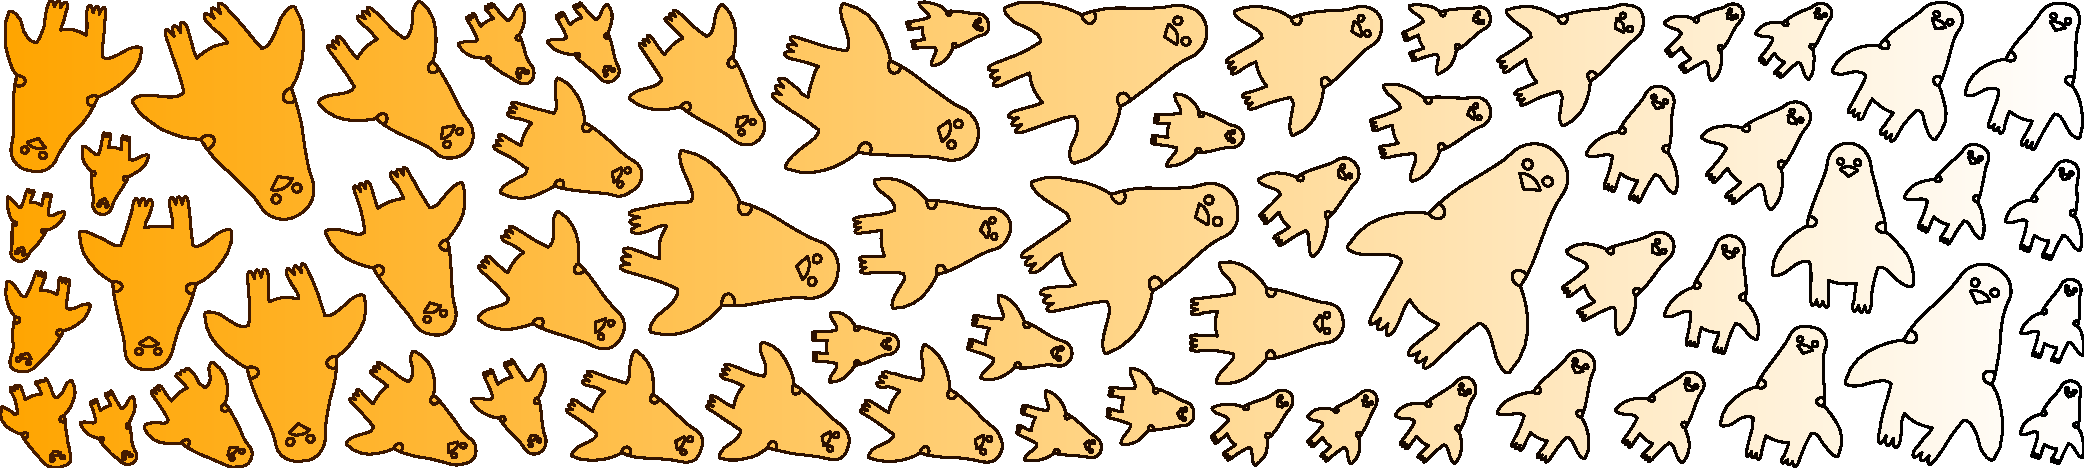
\includegraphics[width=1.0\textwidth]{figures/repulsionpak/giraffe_penguin.pdf}
\caption[A packing that demonstrates torsional forces]
{\label{giraffe_penguin_packing}
A packing that demonstrates torsional forces.
The packing uses copies of a single element shape, but every copy is given a rest orientation between $0^\circ$
and $180^\circ$, based on its horizontal position in the container.  In the final packing the elements transition
from upright to upside-down, recreating an illusion in which giraffe heads become penguins.}
\end{figure*}

%\begin{minipage}{\textwidth}
\begin{figure}
\centering
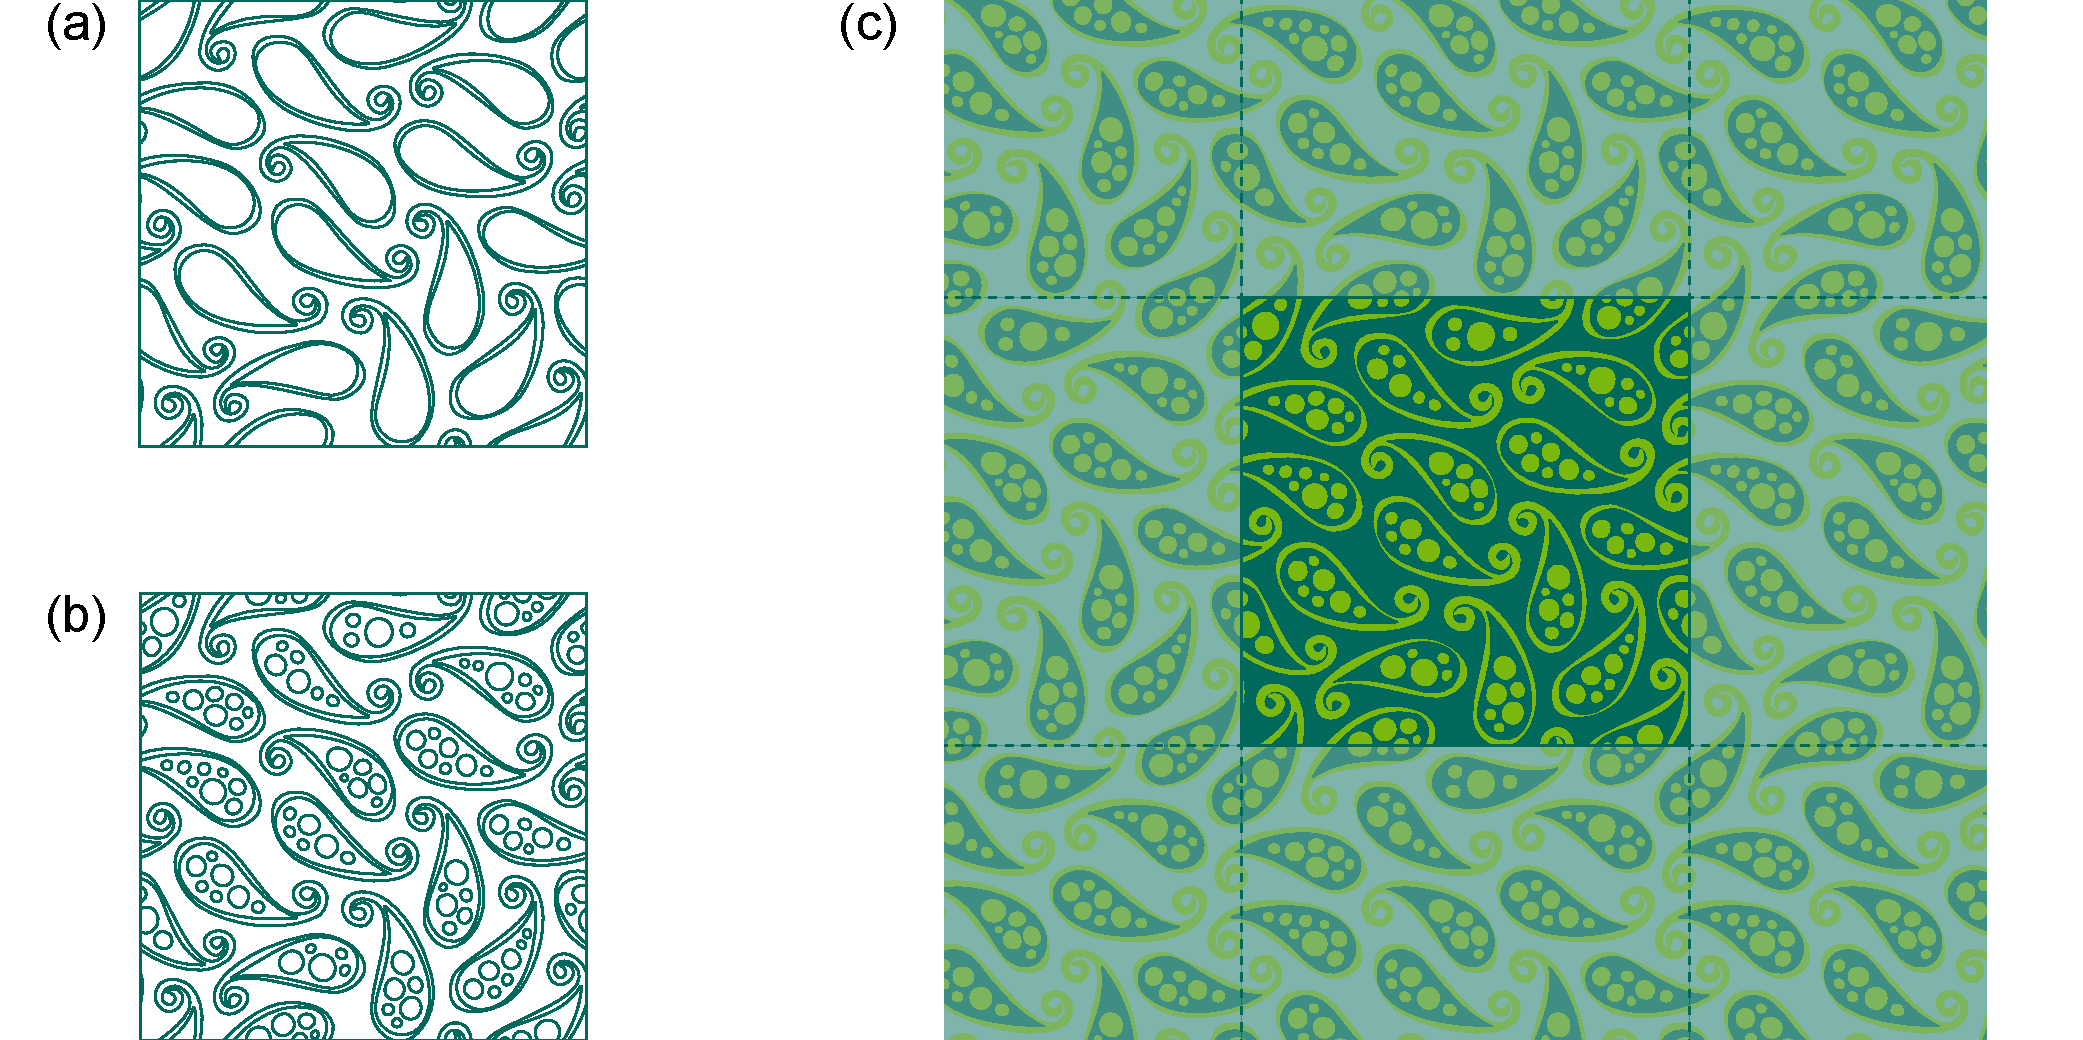
\includegraphics[width=0.95\columnwidth]{figures/repulsionpak/paisley_new.pdf} 
\vspace{-10pt}
\caption[A paisley-inspired toroidal packing that can tile the plane]
{\label{paisley_packing}
A paisley-inspired toroidal packing that can tile the plane. 
           (a) An initial paisley packing.
           (b) In a separate simulation, we fill each paisley with circles to demonstrate a packing inside a packing.
           (c) The final result.
}
\end{figure}

\begin{figure}
\centering

\includegraphics[width=0.85\columnwidth]{figures/repulsionpak/bad_results.pdf} 
\vspace{-12pt}
\caption[Two demonstrations of how extreme parameter values can lead to \newline 
	low-quality results]
	{\label{bad_results}
Two demonstrations of how extreme parameter values can lead to
	low-quality results.  In~(a), we allow repulsion to overwhelm element
	shape by setting $k_r$ to 200 and $k_e$ to 20; the resulting packing 
	has even negative space, but elements suffer from high deformation
	and self intersections.  In~(b), we minimize repulsion and prioritize
	orientation by setting $k_e$, $k_t$, and $k_r$ to 200, 100, and 50,
	respectively.  The elements deviate minimally from their original shapes 
	and orientations, but cannot fill the container effectively.
}
\end{figure}

\begin{table}[h]
\centering 
\caption[Data and statistics for the RepulsionPak results]
{
   Data and statistics for the RepulsionPak results.  The table shows the
   numbers of primary and secondary elements ($n_p$, $n_s$),
   the number of vertices ($v$), 
   the running times of the primary and the secondary simulations ($t_p$, $t_s$) in seconds,
   and the number of iterations ($i$).
   In these results, torsional forces are used only in 
   Fig.~\ref{giraffe_penguin_packing} and shape matching is used only 
   in Fig.~\ref{rhino_packing}.
   }
\label{packing_statistics}
\definecolor{lg}{rgb}{0.73,0.867,0.98}
\vspace{-10pt}
\resizebox{\columnwidth}{!}{
\begin{tabular}{|l|c|c|c|c|c|c|}
\hline
\cellcolor{lg}Packing                  & \cellcolor{lg}$n_p$ & \cellcolor{lg}$n_s$ & \cellcolor{lg}$v$   & \cellcolor{lg}$t_p$ & \cellcolor{lg}$t_s$ & \cellcolor{lg}$i$\\ \hline
Animals (Fig.~\ref{pipeline})                       & 25    & 14   & 2412  & 133  & 65  & 16670\\ \hline
\newtext{Rhino   (Fig.~\ref{rhino_packing})}        & 107   & 0    & 4833  & 237  & 0   & 15521\\ \hline
Cats (Fig.~\ref{cat_packing})                       & 41    & 69   & 3598  & 185  & 62  & 8531\\ \hline
Birds  (Fig.~\ref{three_packings}a)                 & 43    & 43   & 2309  & 102  & 54  & 11571\\ \hline
Bats (Fig.~\ref{three_packings}b)                   & 47    & 22   & 3048  & 165  & 56  & 13120\\ \hline
Butterflies (Fig.~\ref{three_packings}c)            & 123   & 135  & 11916 & 696  & 616 & 14379\\ \hline
\newtext{Giraffes \& Penguins (Fig.~\ref{giraffe_penguin_packing})}        & 60    & 0   & 2250  & 163  & 0   & 9347\\ \hline
\newtext{Paisley (Fig.~\ref{paisley_packing})}      & 162   & 0    & 4860  & 128  & 0   & 23040\\ \hline
\newtext{Circles in Paisleys (Fig.~\ref{paisley_packing})}      & 144   & 0    & 2544  & 403  & 0   & 29584\\ \hline
\newtext{Collage (Fig.~\ref{pad_comparison})}       & 51    & 0    & 3481  & 729  & 0   & 29868\\ \hline
\newtext{Autumn  (Fig.~\ref{balabolka_comparison})} & 77    & 0    & 2427  & 868  & 0   & 38387\\ \hline
\end{tabular}
} 
\end{table}


Our software was written in C++, and reads in text files describing
elements and containers; we prepared these files using
Adobe Illustrator.  We ran
our software on a computer with a 2.4 GHz Intel i7-4700HQ processor
and 16 GB of RAM.  As a post-process, we optionally read packings
back into Illustrator, fit smooth curves to polygonal paths, and
apply colours and other visual effects.  Table~\ref{packing_statistics}
shows statistics for the results in the paper.  All results in this
paper use $\Delta t = 0.1$.
Torsional forces are used only in Fig.~\ref{giraffe_penguin_packing},
and shape matching is used only in Fig.~\ref{rhino_packing}.
We also use our improved method for resolving self intersection in
Figs.~\ref{rhino_packing},~\ref{giraffe_penguin_packing},
~\ref{paisley_packing},
~\ref{pad_comparison}, and
~\ref{balabolka_comparison}.

The supplemental materials include movies that visualize the simulation
process.  These movies make it clear that elements can jostle each other
around, inducing translation, rotation, and deformation throughout the 
simulation.

The packing in Fig.~\ref{cat_packing} 
uses six cat-shaped primary elements and one secondary cat head.
RepulsionPak naturally bends legs and tails to fill the container more evenly.

The animal packing in Fig.~\ref{pipeline} 
has several elements with limbs (the bear, fox, chick, and penguin),  
extensions (the dog and bunny ears), and long shapes (the snake).
Fig.~\ref{fig_defviz} highlights the deformations for some of these elements;
they are noticeably more deformed 
than nearly convex elements like the cat and mouse.


The butterfly packing in Fig.~\ref{three_packings} is an attempt to reproduce 
the visual style of a 
dense packing (or tessellation), similar to Jigsaw Image Mosaics~\cite{Kim2002}
or the ``Butterflies in Butterfly'' example from the
Pyramid of Arclength Descriptor paper~\cite[Fig. 21]{Kwan2016}. 
The target container is made from two regions,
one with internal holes.  The resulting packing is tight but overlap-free.

The packing on the left in Fig.~\ref{three_packings}
exhibits significant deformation in the wings and the tails of the birds.
In particular, the thin tails of the swallows have some unaesthetic
sharp bends.  We would like to investigate ways to ensure these bends are
smoother.

The packing in Fig.~\ref{giraffe_penguin_packing} demonstrates torsional forces
that gradually turn the elements upside down. 
The rhinoceros packing in Fig.~\ref{rhino_packing} demonstrates initial placement via shape matching.
The entire shape matching process took 922 milliseconds with a 4-element library.

We have also experimented with creating tileable packings, as shown
in Fig.~\ref{paisley_packing}.  We seed a central square with elements,
but also place clones of those elements in all the squares of the
8-neighbourhood around the center.  These clones track the transformations
and deformations of their originals, but also exert forces on them during
simulation, leading to an even, seamless packing in a toroidal domain.

We have found that RepulsionPak is robust to parameter variation, and 
produces predictable, high quality results without the need for fine-grained
adjustments.  However, as shown in Fig.~\ref{bad_results}, extreme parameter 
settings can still produce degenerate results.
In Fig.~\ref{bad_results}a, the repulsion force is made much stronger than 
the edge force, leading to excessive element deformation and
self-intersections in the pursuit of even negative space.  In 
Fig.~\ref{bad_results}b, edge and torsional forces dominate repulsion,
producing a packing with stiff, upright elements that do not fill their
container effectively.


%%%%%%%%%%%%%%%%%%%%%%%%%%%%%%%%%%%%%%%%%%%%%%%%%%%%%%%%%%
%%%%%%%%%%%%%%%%%%%%%%%%%%%%%%%%%%%%%%%%%%%%%%%%%%%%%%%%%%
\section{Conclusions}
\label{repulsionpak_conclusions}
%%%%%%%%%%%%%%%%%%%%%%%%%%%%%%%%%%%%%%%%%%%%%%%%%%%%%%%%%%
%%%%%%%%%%%%%%%%%%%%%%%%%%%%%%%%%%%%%%%%%%%%%%%%%%%%%%%%%%

\mynote{need to move a few sentences to evaluation}

We presented RepulsionPak, a method to create packings with deformable elements.
The combination of repulsion forces and controlled deformation
allows RepulsionPak to discover shape compatibilities that
eliminate the need for a large element library
and fill the target container effectively.
\newtext{
Our compositions have negative space between elements that
is approximately uniform in width, and we validate our approach using overlap functions,
spherical contact probability functions, and distance histograms.
}

We see many possibilities for further improvements to RepulsionPak
and future research on element packings.


\begin{itemize}
\item 
	Because our main goal was to demonstrate the validity of a 
	deformation-driven approach, and not to contribute a new
	physical simulation method, we deliberately chose a simple 
	simulation model based on springs and forward Euler integration.
	Contemporary research has yielded many more sophisticated 
	physical simulation methods, such as Position Based Dynamics~\cite{Muller2007}, 
	Projective Dynamics~\cite{Bouaziz2014}, and the Finite Element Method.
	No one method is obviously best suited to this problem, and
	we intend to experiment with several to investigate if any offers
	a suitable trade-off between performance and quality.

\item We would like to explore the use of RepulsionPak in a fabrication context.
      For example, our boundary compatibilities might be used to create a connected object.
      Alternatively, it would be interesting to 3D print the 
      negative space, which is already connected,
	  leaving holes that surround the element shapes.

\item Our barycentric warping method can
	introduce undesirable artifacts in highly deformed elements, as
	in the swallow tails in the left result of Fig.~\ref{three_packings}.
	We would like to explore other methods for warping an element's
	geometry based on the correspondences between the triangles of its original
	mesh and the deformed meshes in the final packing, based for example on the
	work of Jacobson et al.~\cite{Jacobson2011} and Liu et al.~\cite{Liu2014}.

\end{itemize}
%%%%%%%%%%%%%%%%%%%%%%%%%%%%%%%%%%%%%%%%%%%%%%%%%%%%%%%%%%
%%%%%%%%%%%%%%%%%%%%%%%%%%%%%%%%%%%%%%%%%%%%%%%%%%%%%%%%%%
\chapter{AnimationPak: Packing Elements with Scripted Animations}
\label{chapter_animationpak}
%%%%%%%%%%%%%%%%%%%%%%%%%%%%%%%%%%%%%%%%%%%%%%%%%%%%%%%%%%
%%%%%%%%%%%%%%%%%%%%%%%%%%%%%%%%%%%%%%%%%%%%%%%%%%%%%%%%%%

\begin{figure*}[h!]
  \centering
  \vspace{-30pt}
  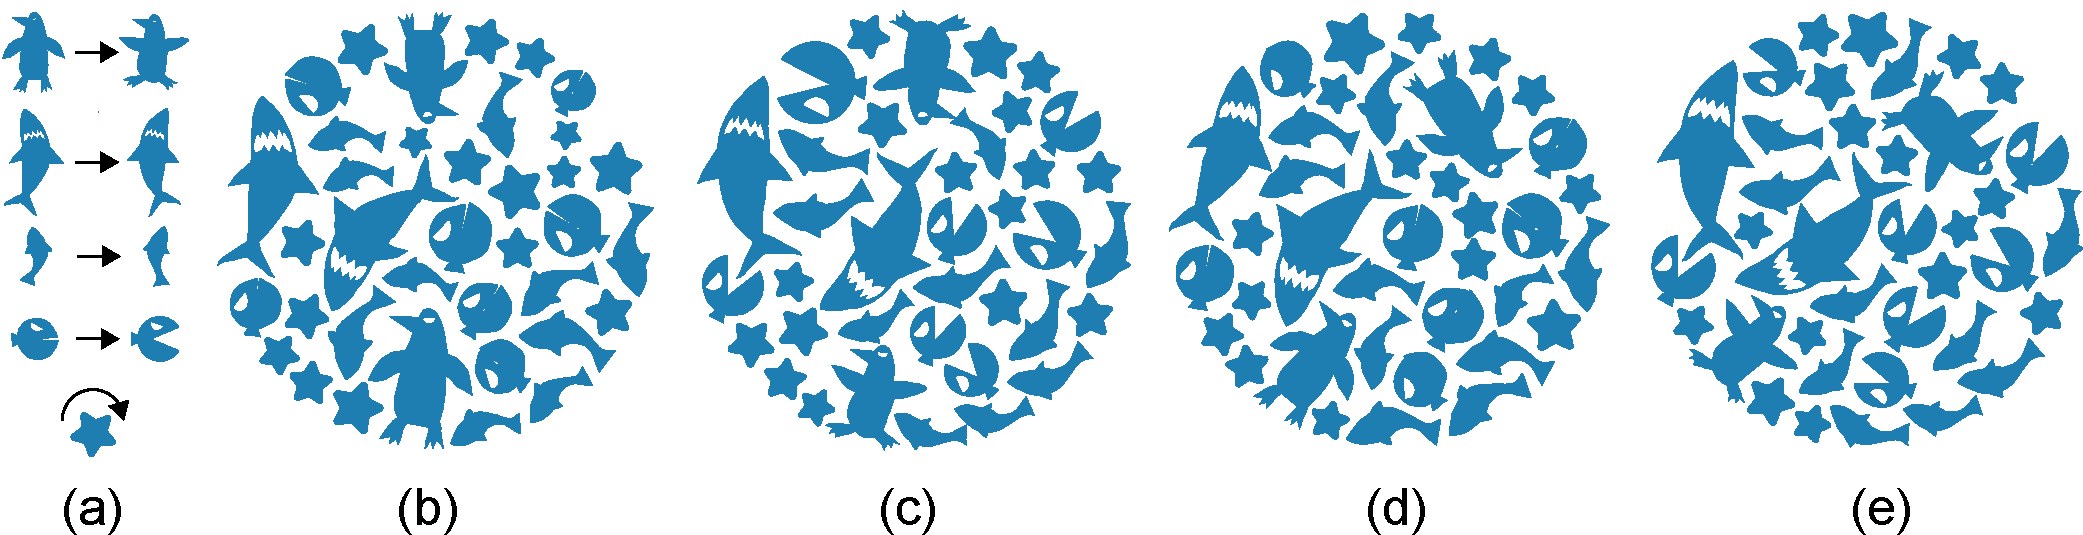
\includegraphics[width=1.0\textwidth]{figures/animationpak/teaser.pdf}
  \caption[An animated packing of aquatic fauna]
  {\label{fig_animationpak_teaser}
  (a) Input animated elements,
  each with its own animation: swimming penguins, swimming sharks and fish,
  Pac-Man fish that open or close their mouths, and rotating stars. 
  (b-e) four selected frames from an animated packing.  
  }
\end{figure*}



%%%%%%%%%%%%%%%%%%%%%%%%%%%%%%%%%%%%%%%%%%%%%%%%%%%%%%%%%%
%%%%%%%%%%%%%%%%%%%%%%%%%%%%%%%%%%%%%%%%%%%%%%%%%%%%%%%%%%
\section{Introduction}
\label{animationpak_introduction}
%%%%%%%%%%%%%%%%%%%%%%%%%%%%%%%%%%%%%%%%%%%%%%%%%%%%%%%%%%
%%%%%%%%%%%%%%%%%%%%%%%%%%%%%%%%%%%%%%%%%%%%%%%%%%%%%%%%%%


AnimationPak is a method to pack elements with scripted animations.
An element can have an animated deformation, \newtext{such as a slithering snake or a dancing bear}.
It can also have an animated transformation, giving a changing
position, size, and orientation within the container.
Our goal is producing an \textit{animated packing}, with elements
playing out their animations while simultaneously filling the
container shape evenly.  A successful animated packing should balance
among the evenness of the negative space, the preservation of 
element shapes, and the comprehensibility of their scripted animations.

We consider an animated
element to be a geometric extrusion along a time axis, a three-dimensional
object that we call a ``spacetime element''.  We use a three-dimensional physical simulation
similar to RepulsionPak to pack spacetime
elements into a volume created by extruding a static container shape.
The animated packing emerges from this three-dimensional volume by rendering 
cross sections perpendicular to the time axis.

\newtext
{
Animated packings are a largely unexplored style
of motion graphics, presumably because of the difficulty of creating 
an animated packing by hand.  
Finding motivating examples created by artists is difficult, and
we only found a single animated packing shown in Figure~\ref{fig_animationpak_lisa_packing},
which is animated gear-like meshing of copies of Lisa Simpson's spiky head.
The discussion in Section~\ref{animationpak_previous_work} shows there is also limited past research
on animated packings.
}



%%%%%%%%%%%%%%%%%%%%%%%%%%%%%%%%%%%%%%%%%%%%%%%%%%%%%%%%%%
%%%%%%%%%%%%%%%%%%%%%%%%%%%%%%%%%%%%%%%%%%%%%%%%%%%%%%%%%%
\section{Related Work}
\label{animationpak_previous_work}
%%%%%%%%%%%%%%%%%%%%%%%%%%%%%%%%%%%%%%%%%%%%%%%%%%%%%%%%%%
%%%%%%%%%%%%%%%%%%%%%%%%%%%%%%%%%%%%%%%%%%%%%%%%%%%%%%%%%%

%\mynote{Only discuss papers whose ideas you use or you're comparing with}

\textbf{Packings and Mosaics:} 
Researchers have explored many approaches to creating 2D packings and
simulated mosaics, including using Centroidal Area Voronoi Diagrams (CAVDs) to
position elements~\cite{Hausner2001,Hiller2003,Smith2005}, spectral
approaches to create even negative space~\cite{Dalal2006}, energy
minimization~\cite{Kim2002}, and shape descriptors~\cite{Kwan2016}.
%\newtext
%{
%Chapter~\ref{chapter_related_work} 
%provides a complete list of research in 2D packings.
%}

\begin{figure}[t]
\centering
\includegraphics[width=1.0\textwidth]{figures/animationpak/lisa_packing.pdf} 
\caption[An animated packing of copies of Lisa Simpson]
{\label{fig_animationpak_lisa_packing} 
\newtext{Three frames of an animated packing from The Simpsons Season 31, Episode 19 ($\copyright$ FOX), showing
gear-like meshing of oppositely-rotating copies of Lisa Simpson.}}
\end{figure}

\textbf{Animated Packings and Tilings:}
Animosaics by Smith et al.~\cite{Smith2005} constructed animations 
in which static elements without scripted
animations follow the motion of an animated container.  Elements are
placed using CAVDs, and advected frame-to-frame using a choice of methods
motivated by Gestalt grouping principles.
As the container's area changes, elements are added and removed as needed,
while attempting to maximize overall temporal coherence.
Dalal et al.~\cite{Dalal2006} showed how the spectral approach they
introduced for 2D packings could be extended 
to pack animated elements in a static container.  Like us, they recast
the problem in terms of three-dimensional spacetime; they compute optimal
element placement using discrete samples over time and orientation.
However, their spacetime elements have fixed
shapes and are made to fit together using only translation and rotation, 
limiting their ability to consume the container's negative space.

Liu and Veksler created animated decorative mosaics from video
input~\cite{Liu2009}.  Their technique combines vision-based
motion segmentation with a packing step similar to Animosaics.
Kang et al.~\cite{Kang2011} extracted edges from video and 
then oriented rectangular tesserae relative to edge directions.

Kaplan~\cite{Kaplan2019} explored animations of simple tilings of
the plane from copies of a single shape.  Elements in a tiling
fit together by construction, and therefore always consume all 
the negative space in the animation.


\newtext{
\textbf{3D Packings:} 
AnimationPak fills a 3D container with 3D elements, 
and is therefore related to approaches that construct 3D
packings, although the time axis in the spacetime domain 
behaves differently than the third spatial axis.
Related work includes 3D collages methods~\cite{Gal2007B, Theobalt2007, Huang2014},
cutting and packing methods~\cite{Chernov2010, Vanek2014, Chen2015}, 
non-overlapping 3D element packing methods~\cite{Byholm2009,Ma2018},
and packing methods for engineering purposes~\cite{Cagan2002}.
} 
%Gal et al.~\cite{Gal2007B} presented a method for constructing 3D
%collages reminiscent of portrait paintings by Arcimboldo.  They
%filled a 3D container with overlapping 3D elements using a greedy
%approach and a partial shape matching algorithm.
%Attene~\cite{Attene2015} decomposed a 3D model into parts that pack
%tightly into a small build volume, allowing it to 
%be 3D printed with less waste material and packed into a smaller box.
%Ma et al.~\cite{Ma2018} developed a heuristic method
%to create 3D packings that are overlap free.  Other work has 
%experimented with example-based packing of 3D volumes~\cite{Ma2011},
%or optimized placement based on user interaction~\cite{Hsu2020}.
%\newtext{Several approaches have been proposed to extend 2D packing methods to adapt to
%the challenges of placing them on the surfaces of 3D 
%objects.~\cite{Hu2016,Chen2016,Zehnder2016,Chen2017}.}

\newtext
{
\textbf{Animated 3D Collages:} Theobalt et al.~\cite{Theobalt2007}
developed a data-driven method to generate animated 3D collages that resemble an Arcimboldo's paintings by arranging 
static 3D elements into an animated 3D container.
They partition the input animated container by identifying
rigid parts, each is replaced by a matching element taken from a library.
The result is a 3D collage with overlapping elements, 
and the animation is created from rigid transformations of the elements.
}


\newtext{
\textbf{Animated Textures:}
Ma et al.~\cite{Ma2013} developed Dynamic Element Textures (DET), a method
to synthesize animated textures of a group of identical elements, such as shoals or particles.
For each animated element in a small exemplar, they generate sample points
both in spatial and temporal domains.
DET generates a larger texture by copying and distributing the sample points,
which are then repositioned to resemble the original distribution in the exemplar.
Similar to DET, AnimationPak represent an animated element as a collection of discrete vertices that
reside in a spacetime domain. However, as a texture synthesis method,
the goal of DET is to distribute elements, and not fill a container tightly.
}

\textbf{Derived Animations:} 
AnimationPak falls into the category of systems that create a derived
animation based on some input animation. This problem, which
requires preserving the visual character of the input, is a 
longstanding one in computer graphics research.
Spacetime constraints~\cite{Witkin1988, Cohen1992} allow an animator
to specify an object's constraints and goals, and then calculates 
the object's trajectory via spacetime optimization.
Motion warping~\cite{Witkin1995} is a method that deforms an existing
motion curve to meet user-specified constraints.
Gleicher~\cite{Gleicher2001} developed a motion path editing method
that allows user to modify the traveling path of a walking character.
Bruderlin and Williams~\cite{Bruderlin1995} used signal processing techniques
to modify motion curves.


Previous work has also investigated geometric deformation of 
animations.
Ho et al. ~\cite{Ho2010} encoded spatial joint relationships 
using tetrahedral meshes, and applied as-rigid-as-possible shape deformation
to the mesh to retarget animation to new characters.
Choi et al.~\cite{Choi2011} developed a method to deform character motion
to allow characters to navigate tight passages.
Masaki~\cite{Oshita2017} developed a motion editing tool that deformed
3D lattice proxies of  a character's joints.
Dalstein et al.~\cite{Dalstein2015} presented a data structure
to animate vector graphics with complex topological changes.
Kim et al.~\cite{Kim2012} explored a packing algorithm
to avoid collisions in a crowd of moving characters.
They defined a motion patch containing temporal trajectories of interacting
characters, and arranged deformed patches to prevent collisions between
characters.




%%%%%%%%%%%%%%%%%%%%%%%%%%%%%%%%%%%%%%%%%%%%%%%%%%%%%%%%%%
%%%%%%%%%%%%%%%%%%%%%%%%%%%%%%%%%%%%%%%%%%%%%%%%%%%%%%%%%%
\section{Animated Elements}
\label{animationpak_animated_element}
%%%%%%%%%%%%%%%%%%%%%%%%%%%%%%%%%%%%%%%%%%%%%%%%%%%%%%%%%%
%%%%%%%%%%%%%%%%%%%%%%%%%%%%%%%%%%%%%%%%%%%%%%%%%%%%%%%%%%



The input to AnimationPak is a library of animated elements and a
fixed container shape.  AnimationPak currently supports two kinds
of animation: the user can animate the shape of each individual
element and can also give elements trajectories that animate
their position within the container.  This
section explains how we animate the element shapes using
as-rigid-as-possible deformation, and then construct
spacetime-extruded objects that form the basis of our packing
algorithm.  These elements animate ``in place'': they change
shape without translating. The next section describes how these
elements can be given transformation trajectories within the
container. Size and orientation of an element can be animated
either way; they can be specified as an animation of the element's
shape, or they can be part of the transformation trajectory.





%%%%%%%%%%%%%%%%%%%%%%%%%%%%%%%%%%%%%%%%%%%%%%%%%%%%%%%%%%
%%%%%%%%%%%%%%%%%%%%%%%%%%%%%%%%%%%%%%%%%%%%%%%%%%%%%%%%%%
\subsection{Spacetime Extrusion}
\label{animationpak_spacetime_extrusion}
%%%%%%%%%%%%%%%%%%%%%%%%%%%%%%%%%%%%%%%%%%%%%%%%%%%%%%%%%%
%%%%%%%%%%%%%%%%%%%%%%%%%%%%%%%%%%%%%%%%%%%%%%%%%%%%%%%%%%

Each element begins life as a static shape defined using
vector paths.  \newtext{Similar to RepulsionPak}, we construct a discrete
geometric proxy of the element that will interact with other
proxies in a physical simulation.  The construction of this proxy
for a single shape is shown in Figure~\ref{fig_animationpak_discretization}, and
the individual steps are explained in greater detail below.

In order to produce a packing with an even distribution of negative
space, we first offset the shape's paths by a distance $\Delta s$,
leaving the shape surrounded by a channel of negative space
(Figure~\ref{fig_animationpak_discretization}a).  In our system
we scale the shape to fit a unit square and set $\Delta s=0.04$.

\newtext
{
Next, we place evenly-spaced samples around the outer boundary of 
the offset path and construct a Delaunay triangulation of the samples
(Figure~\ref{fig_animationpak_discretization}b). We will
later treat the edges of the triangulation as springs, allowing the
element to deform in response to forces in the simulation.  
We also follow RepulsionPak by adding shear edges to prevent
folding and negative-space edges to avoid self-overlaps during simulation
(Figure~\ref{fig_animationpak_discretization}c).
}

We refer to the augmented triangulation shown in 
Figure~\ref{fig_animationpak_discretization}c as a \textit{slice}.  
The entire spacetime packing process operates on slices.  
However, we will eventually
need to compute deformed copies of the element's original vector paths 
when rendering a final animation (Section~\ref{animationpak_rendering}).
To that end, we re-express all path information relative to the
slice triangulation: every path control point is represented using
barycentric coordinates within one triangle.

To extend the element into the time dimension, 
we now position evenly-spaced copies of the slice along the time axis.
Assuming that the animation will run over the time interval $[0,1]$, 
we choose a number of slices $n_s$ and place slices $\{s_1,\ldots,s_{n_s}\}$,
with slice $s_i$ being placed at time $(i-1)/(n_s-1)$.
Higher temporal resolution will
produce a smoother final animation at the expense of more computation.
In our examples, we set $n_s=100$. 
Figure~\ref{fig_animationpak_discretization}d shows a set of time slices, with
$n_s=5$ for visualization purposes.

To complete the construction of a spacetime element without animation,
we stitch the slices together into a single 3D object.  Let $s_j$ and
$s_{j+1}$ be consecutive slices constructed above.  The outer boundaries
of the element triangulations are congruent polygons offset in the time 
axis.  We stitch the two polygons together using a new set of 
\textit{time edges}: if $AB$ is an edge on the boundary of $s_j$ and
$CD$ is the corresponding edge on the boundary of $s_{j+1}$, then
we add time edges $AC$, $AD$, and $BC$.
During simulation, time edges will transmit forces backwards and forwards in
time, maintaining temporal coherence by smoothing out deformation and 
transformations.
Figure~\ref{fig_animationpak_discretization}e shows time edges for $n_s=5$.

\begin{figure*}
\centering
\includegraphics[width=1.0\textwidth]{figures/animationpak/discretization.pdf} 
\caption[The creation of a discretized spacetime element]
{\label{fig_animationpak_discretization} 
The creation of a discretized spacetime element.  
(a) A 2D element shape offset by $\Delta s$.
(b) A single triangle mesh slice.
(c) Shear edges (red) and negative space edges (blue).
(d) A set of five slices placed along the time axis.
(e) The vertices on the boundaries of the slices are joined by 
  time edges.  The black edges in~(e) define a triangle mesh
  called the envelope of the element.
  In practice we use a larger number of slices in~(d) and~(e).
}
\end{figure*}

\begin{figure}
\centering
\includegraphics[width=1.0\textwidth]{figures/animationpak/spacetime_element.pdf} 
\caption[A spacetime element with a scripted animation]
{\label{fig_animationpak_spacetime_element} 
A spacetime element with a scripted animation.}
\end{figure}


%%%%%%%%%%%%%%%%%%%%%%%%%%%%%%%%%%%%%%%%%%%%%%%%%%%%%%%%%%
%%%%%%%%%%%%%%%%%%%%%%%%%%%%%%%%%%%%%%%%%%%%%%%%%%%%%%%%%%
\subsection{Animation}
\label{animationpak_animation}
%%%%%%%%%%%%%%%%%%%%%%%%%%%%%%%%%%%%%%%%%%%%%%%%%%%%%%%%%%
%%%%%%%%%%%%%%%%%%%%%%%%%%%%%%%%%%%%%%%%%%%%%%%%%%%%%%%%%%

The 3D information constructed above is a parallel extrusion of a 
slice along the time axis, representing a shape with no scripted animation.
We created a simple interactive application for adding animation to
spacetime elements, inspired by as-rigid-as-possible shape
manipulation~\cite{Igarashi2005}.  The artist first designates a subset
of the slices as keyframes.  They can then interactively manipulate
any triangulation vertex of a keyframe slice.  Any vertex that has
been positioned manually has its entire trajectory through the animation
computed using spline interpolation.  Then, at any other slice, the positions
of all other vertices can be interpolated using the as-rigid-as-possible
technique.  The result is a smoothly animated spacetime volume like the one
visualized in Figure~\ref{fig_animationpak_spacetime_element}.

\newtext{Unlike data-driven packing methods, AnimationPak allows 
distortions so it does not require a large library of distinct elements
to generate successful packings.}  The results in this paper all use
fewer than ten input elements, and some use only one.
The physical simulation induces deformation to enhance 
the compatibility of nearby shapes in the final animation.

%%%%%%%%%%%%%%%%%%%%%%%%%%%%%%%%%%%%%%%%%%%%%%%%%%%%%%%%%%
%%%%%%%%%%%%%%%%%%%%%%%%%%%%%%%%%%%%%%%%%%%%%%%%%%%%%%%%%%
\section{Initial Configuration}
\label{animationpak_initial_configuration}
%%%%%%%%%%%%%%%%%%%%%%%%%%%%%%%%%%%%%%%%%%%%%%%%%%%%%%%%%%
%%%%%%%%%%%%%%%%%%%%%%%%%%%%%%%%%%%%%%%%%%%%%%%%%%%%%%%%%%



We begin the packing process by constructing a 3D spacetime volume for
the container by extruding its static shape in
the time direction.  The container is 
permitted to have internal holes, which are also extruded.  
The resulting volume is scaled to fit a unit cube.
We also shrink each of the spacetime elements, in the spatial dimensions
only, to 5--10\% of its original size.  These shrunken elements are 
thin enough that we can place them in the container without overlaps.


The artist can optionally specify 
trajectories for a subset of the elements, which we call \textit{guided
elements}.  A guided element attempts to pass through a sequence
of fixed target points in the container,
imbuing the animation with a degree
of intention and narrative structure.  To define a guided element,
we designate the triangulation vertex closest to its centroid
to be the anchor point for the element.  The artist then
chooses a set of spacetime target points $\bm{p}_1,\ldots,\bm{p}_n$,
with $\bm{p}_i=(x_i,y_i,t_i)$, that the anchor should pass through
during the animation.
In our interface, the artist uses a slider to choose the time $t_i$ for 
a target point, and clicks in the container to specify the spatial
position $(x_i,y_i)$.
The artist can also optionally specify scale and
orientation at the target points. We require $t_1=0$ and $t_n=1$,
fixing the initial and final positions of the guided element.  
We then linearly interpolate the anchor position
for each slice based on the target points, and translate the slice
so that its anchor lies at the desired position.  The red extrusions
in Figure~\ref{fig_animationpak_simulation_process}a are guided elements.

If the artist wishes to create a looping animation, the $(x_i,y_i)$ position
for target points $\bm{p}_1$ and $\bm{p}_n$ must match up, either
for a single guided element or across elements. In
Figure~\ref{fig_animationpak_simulation_process} the two guided elements form a connected
loop; $(x_1,y_1)$ for each one matches $(x_n,y_n)$ for the other.

In this initial configuration, the guided elements abruptly change
direction at target points.  However, because the slices are connected
by springs, the trajectories will smooth out as the 
simulation runs. Also, the simulation is not constrained to reach
each target position exactly.  Instead, we attach the
anchor to the target using a \textit{target-point spring} that
attempts to draw the element towards it while balancing against
the other physical forces in play (Figure~\ref{fig_animationpak_simulation_process}b).
The strength of these springs determines how closely the element
will follow the trajectory.

We then seed the container with an initial packing of non-guided
spacetime elements.  We generate points within the container at random, 
using blue-noise sampling~\cite{Bridson2007}
to prevent points from being too close together,
and assign a spacetime element to
each seed point, selecting elements randomly from the input library.
Depending upon the desired effect, we either randomize their orientations
or give them preferred orientations.  We reject any candidate seed point
that would cause an unguided element's volume to intersect a guided element's
volume.

Finally we shrink each element, guided and unguided, uniformly in the spatial dimension
towards its centroid.  These shrunken elements are
guaranteed not to intersect one another; as the simulation runs, they
will grow and consume the container's negative space, while avoiding
collisions.
The blue extrusions in Figure~\ref{fig_animationpak_simulation_process}a show an
initial placement of spacetime elements.

\begin{figure}
\centering
\includegraphics[width=1.0\textwidth]{figures/animationpak/guided_element.pdf} 
\caption[A 2D illustration of a guided element]{
\label{fig_animationpak_guided_element} A 2D illustration of a guided element.
Slices are depicted as black lines and slice vertices as black dots.
A spring connects the centermost vertex $\bm{x}$ of a slice $s$ to a target
point $p$.
(a) The initial shape of a guided element is a polygonal extrusion.
(b) The spacetime element deforms but the springs pull it back towards
the target points.}
\end{figure}




%%%%%%%%%%%%%%%%%%%%%%%%%%%%%%%%%%%%%%%%%%%%%%%%%%%%%%%%%%
%%%%%%%%%%%%%%%%%%%%%%%%%%%%%%%%%%%%%%%%%%%%%%%%%%%%%%%%%%
\section{Simulation}
\label{animationpak_simulation}
%%%%%%%%%%%%%%%%%%%%%%%%%%%%%%%%%%%%%%%%%%%%%%%%%%%%%%%%%%
%%%%%%%%%%%%%%%%%%%%%%%%%%%%%%%%%%%%%%%%%%%%%%%%%%%%%%%%%%

%\subsection{Forces}
%\label{animationpak_forces}

\begin{figure}[h]
\vspace{-20pt}
\centering
\includegraphics[width=1.0\textwidth]{figures/animationpak/simulation_process.pdf} 
\caption[An illustration of the AnimationPak simulation process]{
\label{fig_animationpak_simulation_process} The simulation process. 
(a) Initial placement of 
shrunken spacetime elements inside a static 2D disc, extruded into a 
cylindrical spacetime domain.
Guided elements are shown in red and unguided elements in blue.
(b) A physics simulation causes the spacetime elements to bend. They
also grow gradually.
(c) The spacetime elements occupy the container space.
(d) The simulation stops when elements do not have sufficient negative
space in which to grow, or have reached their target sizes.
}
\end{figure}

\newtext
{
We perform a physics simulation on the spacetime elements and the 
container.  Elements are \newtext{subjected} to a number of forces that cause them
to simultaneously grow, deform, and repel each other (Figure~\ref{fig_animationpak_simulation_process}).
In Section~\ref{animationpak_slice_constraints} we introduce some new hard
constraints that must be applied after every time step.
Note that we must distinguish two notions of time in this simulation.  We use
$t$ to refer to the time axis of our spacetime volume, which will become
the time dimension of the final animation, and $t_\mathrm{sim}$ to
refer to the time domain in which the simulation is taking place.
}

\newtext
{
Let $\bm{x} = (x, y, t)$ be a vertex of a slice.
The total force $\simforce{total} $ applied to $\bm{x}$ is
\begin{equation}
\simforce{total}  = \simforce{rpl} + \simforce{edg} + \simforce{bdr} + \simforce{ovr} + \simforce{tor} + \simforce{tmp}
\end{equation}
where 
\begin{packeddescriptions}
  \item[$\simforce{rpl}$] is the repulsion force;
  \item[$\simforce{edg}$] is the edge force;
  \item[$\simforce{bdr}$] is the boundary force;
  \item[$\simforce{ovr}$] is the overlap force;
  \item[$\simforce{tor}$] is the torsional force; and 
  \item[$\simforce{tmp}$] is the temporal force.  
\end{packeddescriptions}
%where $\simforce{rpl}$, $\simforce{edg}$, $\simforce{bdr}$, $\simforce{ovr}$,  $\simforce{tor}$ and $\simforce{tmp}$ are 
%the repulsion force, the edge force, the boundary force, the overlap force, the torsional force, and the temporal force.
The these forces are the spacetime analogues of the ones used in RepulsionPak, except the new temporal force.
In this section, we explain the first five forces briefly 
and readers can refer back to Section~\ref{repulsionpak_simulation}
for equations used to generate them.
}



\newtext
{
\textbf{Repulsion forces} allow elements to push away vertices of 
neighboring elements, inducing deformations and transformations that lead 
to an even distribution of elements within the container
(Figure~\ref{fig_animationpak_repulsion_force}).
Since the simulation operates in the spacetime domain,
vertex $\bm{x}$ accumulates repulsion forces from points at
various time positions.
To locate these points on neighboring elements that are considered 
nearest, we use a collision grid data structure, described in greater
detail in Section~\ref{animationpak_spatial_queries}.
}


\begin{figure} 
\centering
\includegraphics[width=1.0\textwidth]{figures/animationpak/repulsion_force.pdf} 
\caption[An illustration of the repulsion forces]
{\label{fig_animationpak_repulsion_force} 
Repulsion forces applied to a vertex $\bm{x}$, 
allowing the element to deform and move away from a neighboring element.}
\end{figure}



\newtext
{
\textbf{Edge forces}
allow elements to deform in response to repulsion forces.
%The edges defined in Section~\ref{animationpak_spacetime_extrusion} are used here as springs.
%We have five types of springs, with stiffness constants that can be 
%set independently.
As discussed in Section~\ref{animationpak_spacetime_extrusion} and Section~\ref{animationpak_initial_configuration},
we have five types of springs:
edge springs,
shear springs,
negative-space springs,
time springs, and
target-point springs.
Each of the spring type has a different relative strength.
}

\newtext
{
\textbf{Overlap forces} resolve a vertex penetrating a
neighboring spacetime element.
Overlaps can occur later in the simulation when negative space is 
limited.  Once we detect a penetration,  
we temporarily disable the repulsion force on vertex $\bm{x}$, and apply
an overlap force $\simforce{ovr}$ to push it out.
}

\newtext
{
\textbf{Boundary forces} keep vertices inside the container.
If an element vertex $\bm{x}$
is outside the container, the boundary force $\simforce{bdr}$ moves
it towards the closest point
on the container's boundary by an amount proportional to the distance to
the boundary.
}

\newtext
{
\textbf{Torsional forces} allow an element's slices to be given
preferred orientations, to which they attempt to return.
}

\newtext
{
\textbf{Temporal forces} prevent slices from drifting too far
from their original positions along the time axis positions
(Figure~\ref{fig_animationpak_t_force}), which could cause unexpected accelerations
and decelerations in the final animation.  For every vertex, we compute
the temporal force $\simforce{tmp}$ as
\begin{equation}
\simforce{tmp} = k_\mathrm{tmp} \bm{u}^t(t - t')
\end{equation}
where
\begin{packeddescriptions}
  \item[$k_\mathrm{tmp}$] is the relative strength of $\simforce{tmp}$;
  \item[$t$] is the initial time of the slice to which the vertex belongs;
  \item[$t'$] is the current time value of the vertex; and
  \item[$\bm{u}^t = (0,0,1)$.]
\end{packeddescriptions}
}

\begin{figure}
\centering
\includegraphics[width=1.0\textwidth]{figures/animationpak/t_force.pdf} 
\caption[An illustration of the temporal forces]
{\label{fig_animationpak_t_force} 
An illustration of the temporal force.  The vertices in slice
$s_i$ are drawn back towards time $t$.
}
\end{figure}

\newtext
{
\textbf{Simulation Details:}
We use explicit Euler integration to simulate the motions of the mesh vertices under the
forces described above.  Every vertex has a position and a velocity vector; in
every iteration, we update velocities using forces, and update positions using
velocities.  These updates are scaled by a time step 
$\Delta t_\mathrm{sim}$ that we set to $0.01$.
We cap velocities at $10 \Delta t_\mathrm{sim}$ 
to dissipate extra energy from the simulation.
}

\newtext
{
The constants $k_\mathrm{rpl}$, $k_\mathrm{ovr}$, $k_\mathrm{bdr}$  $k_\mathrm{edg}$, $k_\mathrm{tor}$ 
and $k_\mathrm{tmp}$ control the relative strengths
of repulsion, overlap, boundary, edge, torsional, and temporal forces, respectively.
%of the six forces in the simulation.  
They must be adjusted relative to the time step $\Delta t_\mathrm{sim}$ and the size of the container.
Since container's bounding box is resized to a unit cube,
we set $k_\mathrm{rpl}=10$, $k_\mathrm{ovr}=k_\mathrm{bdr}=5$, $k_\mathrm{tor}=k_\mathrm{tmp}=1$.
We set $k_\mathrm{edg} = 0.01$ for time springs,
$k_\mathrm{edg} = 0.1$ for negative-space springs, and $k_\mathrm{edg} = 10$ for edge springs, shear springs,
and target-point springs.
}





%%%%%%%%%%%%%%%%%%%%%%%%%%%%%%%%%%%%%%%%%%%%%%%%%%%%%%%%%%
%%%%%%%%%%%%%%%%%%%%%%%%%%%%%%%%%%%%%%%%%%%%%%%%%%%%%%%%%%
\subsection{Spatial Queries}
\label{animationpak_spatial_queries}
%%%%%%%%%%%%%%%%%%%%%%%%%%%%%%%%%%%%%%%%%%%%%%%%%%%%%%%%%%
%%%%%%%%%%%%%%%%%%%%%%%%%%%%%%%%%%%%%%%%%%%%%%%%%%%%%%%%%%



Repulsion and overlap forces rely on being able to find points on
neighboring elements that are close to a given query vertex.
To find these points, we use each element's
\textit{envelope}, a triangle mesh implied by the construction in
Section~\ref{animationpak_spacetime_extrusion}.  Each triangle of the envelope 
is made from two time edges and one edge of a slice boundary, as
shown in Figure~\ref{fig_animationpak_collision_grid}a.  Given a query vertex 
$\bm{x}$, we need to find nearby envelope triangles that belong to
other elements.

To accelerate this computation, we first compute and store the centroids of
every element's envelope triangles in a uniformly subdivided 3D grid that
surrounds the spacetime volume of the animation.  In using this data
structure, we make two simplifying assumptions; first, that because 
envelope triangles are small, their centroids
are adequate for finding triangles near a given query point; and second,
that the repulsion force from a more distant triangle is well approximated
by a force from its centroid.

Given a query vertex $\bm{x}$, we first find all envelope triangle
centroids in nearby grid cells that belong to other elements.  For each 
centroid, we use a method described by Ericson~\cite{Ericson2005} to
find the point on its triangle closest to $\bm{x}$ and
include that point in the list of points in Eq.~(1).  These
nearby triangles will also be used to test for interpenetration of elements.
We then find centroids in more distant grid cells, and add
those centroids directly to the Eq.~(1) list, skipping the closest point computation.
In our system we set the cell size to 0.04, giving a $25\times 25\times 25$
grid around the simulation volume.  A query point's nearby grid cells 
are the 27 cells making up a $3\times 3\times 3$ block around the cell 
containing the point; the more distant cells are the 98 that make up the
outer shell of the $5\times 5\times 5$ block around that 
(Figure~\ref{fig_animationpak_collision_grid}).


\begin{figure}
\centering
\includegraphics[width=1.0\textwidth]{figures/animationpak/collision_grid.pdf} 
\caption[An envelope and a collision grid]
{\label{fig_animationpak_collision_grid} 
(a) The triangles that connect consecutive slices define the envelope of the
element.  The midpoints of these triangles are stored in a collision grid.
(b) A 2D visualization of the region of collision
grid cells around a query point 
$\bm{x}$ 
in which repulsion and overlap forces will be computed.  In the central blue
region, we check overlaps and compute exact repulsion forces relative to
closest points on triangles of neighboring elements; in the peripheral
red region we do not compute overlaps, and repulsion forces are approximated
using triangle midpoints only.}
%% \craig{Do we really need this figure?}
\end{figure}


%%%%%%%%%%%%%%%%%%%%%%%%%%%%%%%%%%%%%%%%%%%%%%%%%%%%%%%%%%
%%%%%%%%%%%%%%%%%%%%%%%%%%%%%%%%%%%%%%%%%%%%%%%%%%%%%%%%%%
\subsection{Slice Constraints}
\label{animationpak_slice_constraints}
%%%%%%%%%%%%%%%%%%%%%%%%%%%%%%%%%%%%%%%%%%%%%%%%%%%%%%%%%%
%%%%%%%%%%%%%%%%%%%%%%%%%%%%%%%%%%%%%%%%%%%%%%%%%%%%%%%%%%

\begin{figure}[h!]
\centering
\includegraphics[width=1.0\textwidth]{figures/animationpak/constraints.pdf} 
\caption[Constraints]
{\label{fig_animationpak_constraints} 
a) End-to-end constraint: 
slice $s_1$ and $s_n$, located at 
$t = 0$ and $t = 1$,  should never change their $t$ positions but can change their $x, y$ positions. 
b) Simultaneity constraint: all vertices on the same slice should have the same $t$ position.
c) Loop constraint with a single element: the $x,y$ positions for $s_1$ and $s_n$ must match.
d) Loop constraint with two elements: the $x, y$ position for $s_1$  
for one element matches the $x, y$ position for $s_n$ of the other.
}
\end{figure}



There are three hard geometric constraints on the configuration of slices,
which must be enforced throughout the simulation.  Each of the following
constraints is reapplied after each physical simulation step described above.

\begin{enumerate}
\item \textbf{End-To-End Constraint:}
A spacetime element must be present for the full length of the animation
from $t=0$ to $t=1$.  After every simulation step, every vertex belonging
to an element's first slice has its $t$ value set to $0$, and every vertex
of the last slice has its $t$ value set to $1$
(Figure~\ref{fig_animationpak_constraints}a).

\item \textbf{Simultaneity Constraint:}
During simulation, the vertices of a slice can drift away from each
other in time, which could lead to rendering artifacts in the animation.
After every simulation step, we compute the average $t$ value of all
vertices belonging to each slice other than the first and last slices, and 
snap all the slice's vertices to that $t$ value 
(Figure~\ref{fig_animationpak_constraints}b).

\item \textbf{Loop Constraint:}
AnimationPak optionally supports looping animations.
When looping is enabled, we must ensure that the $t=0$ and $t=1$ planes
of the spacetime container are identical.  
The $t=1$ slice of every element $e_1$ must then 
coincide with the $t=0$ slice of \textit{some} 
element $e_2$.  We can have $e_1=e_2$ 
(Figure~\ref{fig_animationpak_constraints}c), but more general loops are possible in which
the elements arrive at a permutation of their original configuration
(Figure~\ref{fig_animationpak_constraints}d).  We require only that there is a one-to-one
correspondence between the vertices of the $t=1$ slice of $e_1$ and the
$t=0$ slice of $e_2$.  If $\bm{p}_1=(x_1,y_1,1)\in e_1$ and
$\bm{p}_2=(x_2,y_2,0)\in e_2$
are in correspondence, then after every simulation step we
move $\bm{p}_1$ to $(\frac{x_1+x_2}{2},\frac{y_1+y_2}{2},1)$ and
$\bm{p}_2$ to $(\frac{x_1+x_1}{2},\frac{y_2+y_2}{2},0)$.
\end{enumerate}


%%%%%%%%%%%%%%%%%%%%%%%%%%%%%%%%%%%%%%%%%%%%%%%%%%%%%%%%%%
%%%%%%%%%%%%%%%%%%%%%%%%%%%%%%%%%%%%%%%%%%%%%%%%%%%%%%%%%%
\subsection{Element Growth and Stopping Criteria}
\label{animationpak_element_growth_and_stopping_criteria}
%%%%%%%%%%%%%%%%%%%%%%%%%%%%%%%%%%%%%%%%%%%%%%%%%%%%%%%%%%
%%%%%%%%%%%%%%%%%%%%%%%%%%%%%%%%%%%%%%%%%%%%%%%%%%%%%%%%%%



We begin the spacetime packing process with all element slices scaled
down in $x$ and $y$, guaranteeing that elements do not 
overlap.  As the simulation progresses we gradually grow the slices, 
consuming the negative space around them (Figure~\ref{fig_animationpak_growth}a,b).
A perfect packing would fill the spacetime container completely with the elements.
Because each element wraps the underlying animated shape with a narrow channel
of negative space, this would yield an even
distribution of shapes in the resulting animation.
For real-world elements, the goal of minimizing deformation of irregular 
element shapes will lead to imperfect packings with additional pockets
of negative space.


\textbf{Element Growth:}
We induce elements to grow spatially by gradually increasing the rest 
lengths of their springs.
The initial rest length of each spring is determined by the vertex positions in
the shrunken version of the spacetime element constructed in 
Section~\ref{animationpak_initial_configuration}.
We allow an element's slices to grow independently of each other, which
complicates the calculation of new rest lengths for time springs.
Therefore, we create a duplicate of every shrunken spacetime element
in the container, with a straight extrusion
for unguided elements, and a polygonal extrusion for guided elements.
This duplicate is not part of the simulation; it serves as a reference.
Every element slice maintains a current scaling factor $g$.
When we wish to grow the slice, we increase its $g$ value.
We can compute new rest lengths for all springs by scaling every slice
of the reference element by a factor of $g$ relative to the
slice's centroid, and measuring distances between the scaled vertex
positions.  These new rest lengths are then used as the $\ell$ values
in Equation~\ref{eq_edge_force} to calculate edge forces.

Every element slice has its $g$ value initialized to $1$.  After every
simulation step, if none of the slice's vertices were found to 
overlap other elements we increase that slice's $g$ by 
$0.001 \Delta t_\mathrm{sim}$, where $\Delta t_\mathrm{sim}$ is the 
simulation time step.  If any overlaps are found, then that slice's
growth is instead paused to allow overlap and repulsion forces to give it more
room to grow in later iterations.  
This approach can cause elements to fluctuate in size during the course
of an animation, as slices compete for shifting negative space 
(Figure~\ref{fig_animationpak_growth}).

\textbf{Stopping Criteria:} We halt the simulation when the space between
neighboring elements drops below a threshold.  When calculating 
repulsion forces, we find the distance from every slice vertex
to the closest point in a neighboring element.  The minimum of these
distances over all vertices in an element slice determines that slice's
closest distance to neighboring elements.  We halt the simulation
when the maximum per-slice distance falls below 0.006 (relative to a normalized
container size of 1).  That is, we stop when every slice is touching
(or nearly touching) at least one other element.

In some cases it can be useful to stop early based on cumulative element
growth.  In that case, we set a separate threshold for the slice scaling
factors $g$ described above, and stop when the $g$ values of all
slices exceed that threshold.

\begin{figure}
\centering
\includegraphics[width=1.0\textwidth]{figures/animationpak/growth.pdf} 
\caption[Element growths]
{\label{fig_animationpak_growth} 
A spacetime element shown (a) shrunken at the beginning of the simulation,
and (b) grown later in the simulation. (c) When two elements overlap
somewhere along their lengths, they are temporarily prohibited from growing
there.
}
\end{figure}


%%%%%%%%%%%%%%%%%%%%%%%%%%%%%%%%%%%%%%%%%%%%%%%%%%%%%%%%%%
%%%%%%%%%%%%%%%%%%%%%%%%%%%%%%%%%%%%%%%%%%%%%%%%%%%%%%%%%%
\section{Rendering}
\label{animationpak_rendering}
%%%%%%%%%%%%%%%%%%%%%%%%%%%%%%%%%%%%%%%%%%%%%%%%%%%%%%%%%%
%%%%%%%%%%%%%%%%%%%%%%%%%%%%%%%%%%%%%%%%%%%%%%%%%%%%%%%%%%



The result of the simulation described previously is a packing of spacetime 
elements within a spacetime container.  We can render an
animation frame-by-frame by cutting through this volume at 
evenly spaced $t$ values from $t=0$ to $t=1$, \newtext{as shown in Figure~\ref{fig_animationpak_render}}.  For our results, we
typically render 500-frame animations.


During simulation, a given spacetime element's slices may drift from their
original creation times.  However, time springs keep the sequence
monotonic, and the simultaneity constraint ensures that every slice
is fixed to one $t$ value.  To render this element at an arbitrary
frame time $t_f\in[0,1]$, we find the two consecutive slices whose
time values
bound the interval containing $t_f$ and linearly interpolate the vertex
positions of the triangulations at those two slices to obtain a new
triangulation at $t_f$.  We can then compute a deformed copy of the
original element paths by ``replaying'' the barycentric coordinates 
computed in Section~\ref{animationpak_spacetime_extrusion} relative to the displaced
triangulation vertices.  We repeat this process for every spacetime element
to obtain a rendering of the frame at $t_f$.

This interpolation process can occasionally lead to small artifacts in 
the animation.  A rendered frame can fall between
the discretely sampled slices for two elements at an intermediate time
where physical forces were not computed explicitly.  It is therefore
possible for neighboring elements to overlap briefly during such intervals.

\begin{figure*}
\centering
\includegraphics[width=1.0\textwidth]{figures/animationpak/rendering.pdf} 
\caption[An illustration of rendering spacetime elements]
{\label{fig_animationpak_render} 
\newtext{
An illustration of rendering spacetime elements to generate 2D frames by cutting them
at evenly spaced time values from $t=0$ to $t=1$.
}
}
\end{figure*}


%%%%%%%%%%%%%%%%%%%%%%%%%%%%%%%%%%%%%%%%%%%%%%%%%%%%%%%%%%
%%%%%%%%%%%%%%%%%%%%%%%%%%%%%%%%%%%%%%%%%%%%%%%%%%%%%%%%%%
\section{Implementation and Results}
\label{animationpak_implementation_and_results}
%%%%%%%%%%%%%%%%%%%%%%%%%%%%%%%%%%%%%%%%%%%%%%%%%%%%%%%%%%
%%%%%%%%%%%%%%%%%%%%%%%%%%%%%%%%%%%%%%%%%%%%%%%%%%%%%%%%%%


The core AnimationPak algorithm consists of a C++ program that reads 
in text files describing the spacetime elements and the container, 
and outputs raster images of animation frames.

Large parts of AnimationPak can benefit from parallelism.  In
our implementation we update the cells of the collision grid
(Section~\ref{animationpak_spatial_queries}) in parallel by distributing them
across a pool of threads.  When the updated collision grid is ready,
we distribute the spacetime elements over threads.  We calculate
forces, perform numerical integration, and apply the end-to-end and
simultaneity constraints for each element in parallel.  We must
process any loop constraints afterwards, as they can affect vertices in
two separate elements.

We created the results in this paper using a Windows PC with a 
3.60 GHz Intel i7-4790 processor and 16 GB of RAM.  We used a pool
of eight threads, corresponding to the number of logical CPU cores.
Table~\ref{table_packing_statistics} shows statistics for our results.
Each packing has tens of thousands of vertices and hundreds of thousands
of springs, and requires about an hour to complete.
We enable the loop constraint in all results.  \newtext{This chapter shows selected frames from the
results; see supplemental videos for full animations\footnote{\url{https://cs.uwaterloo.ca/~radhitya/animationpak/videos.zip}}.}

%\begin{comment}
\begin{table}[t!]
\centering 
\caption[Data and statistics for the AnimationPak results]
{
   Data and statistics for the AnimationPak results.  The table shows the
   number of elements,
   the number of vertices, 
   the number of springs, 
    the number of envelope triangles, and 
   the running time of the simulation in hours, minutes, and seconds.
   }
\label{table_packing_statistics}
\definecolor{lg}{rgb}{0.73,0.867,0.98}
\begin{tabular}{|c|c|c|c|c|c|}
\hline
  \cellcolor{lg}Packing &
  \cellcolor{lg}Elements &
  \cellcolor{lg}Vertices & 
  \cellcolor{lg}Springs &
  \cellcolor{lg}Triangles &
  \cellcolor{lg}Time \\ \hline
\makecell{Aquatic fauna  \\ (Figure~\ref{fig_animationpak_teaser})}  
& 37         & 97,800             & 623,634            & 106,000    & 01:06:35        
\\ \hline
\makecell{Snake and bird     \\ (Figure~\ref{fig_animationpak_chasing_bird})}  
& 37         & 58,700             & 370,571            & 58,700   & 01:01:32        
\\ \hline
\makecell{Penguin to giraffe \\ (Figure~\ref{fig_animationpak_penguin_giraffe})}  
& 33         & 124,300            & 824,164            & 143,000    & 01:19:50        
\\ \hline
\makecell{\newtext{Loose bird} \\ (Figure~\ref{fig_bib_entering_star})}  
& 32         & 63,700            & 389,373            & 70,100    & 00:19:24        
\\ \hline
\makecell{Lion               \\ (Figure~\ref{fig_animationpak_lion}b)}  
& 16         & 39,400             & 236,086            & 41,800   & 00:41:56        
\\ \hline
\makecell{Animals            \\ (Figure~\ref{fig_animationpak_repulsionpak_vs_animationpak}b)}  
& 34         & 69,600             & 444,337            & 69,800   & 01:00:19        
\\ \hline
\makecell{Heart stars         \\ (Figure~\ref{fig_animationpak_star_comparison}c)}  
& 26         & 85,200             & 598,218            & 85,800   & 00:23:08        
\\ \hline
\end{tabular}
\end{table}



Figure~\ref{fig_animationpak_teaser} is an animation of aquatic fauna featuring two
penguins as guided elements.  During one loop the penguins move clockwise
around the container, swapping positions at the top and the bottom.
Each ends at the other's starting point, demonstrating a loop constraint
between distinct elements.  All elements are animated, as shown in 
Figure~\ref{fig_animationpak_teaser}a.  Note the coupling between the Pac-Man fish's
mouth and the shark's tail on the left side of the second and fourth frames.

A snake chases a bird around an annular container in 
Figure~\ref{fig_animationpak_chasing_bird}, demonstrating a container with a hole
and giving a simple example of the narrative potential of animated
packings.  Figure~\ref{fig_animationpak_penguin_giraffe} animates the giraffe-to-penguin
illusion shown as a static packing in RepulsionPak.  This example
uses torsional forces to control slice orientations.

\begin{figure}
\vspace{-10pt}
\centering
\includegraphics[width=1.0\textwidth]{figures/animationpak/chasing_bird.pdf} 
\caption[An animated packing of a snake chases a bird]
{\label{fig_animationpak_chasing_bird} 
A snake chasing a bird through a packing of animals.  The snake and bird 
  are both guided elements that move clockwise around the annular 
  container.}
\end{figure}

\begin{figure}
\centering
\includegraphics[width=1.0\textwidth]{figures/animationpak/penguin_giraffe.pdf} 
\caption[An animated packing of the penguins-to-giraffes illusion]
{\label{fig_animationpak_penguin_giraffe} 
Penguins turning into giraffes.  The penguins animate by rotating in place.
Torsional forces are used to preserve element orientations.
Frames are taken at $t=0$, $t=0.125$, $t=0.25$, $t=0.375$, and $t=0.5$. 
}
\end{figure}

\newtext{
Figure~\ref{fig_bib_entering_star} shows 
a guided element as a loose bird which is not constricted inside a container.
The loose bird moves from left to right, passing through a packing of small birds.
As some slices of the loose bird taking up container space,
smaller birds have to stop some of their slice growths prematurely.
This is a demonstration of the benefit of the non-uniform slice growths so that
elements can adapt to changes in container area.
In the rendered 2D animation, the elements have a subtle shrinking-and-expanding effect.
The composition can also tile horizontally, which can be seen in the supplemental video.
}

Figure~\ref{fig_animationpak_lion}a is a static packing of \newtext{lion's mane} created by an artist and
used as an example in FLOWPAK (Chapter~\ref{chapter_flowpak}).  In Figure~\ref{fig_animationpak_lion}b,
we reproduce it with animated elements for the mane.
The orientations of elements follow a vector field inside
the container, and are maintained during the animation by 
torsional forces.
We simulate only half of the packing and reflect it to create the other half.
The facial features were added manually in a post-processing step.

Figure~\ref{fig_animationpak_repulsionpak_vs_animationpak} compares
a static 2D packing created by RepulsionPak with a frame
from an animated packing created by AnimationPak.
The extra negative space in AnimationPak comes partly from the trade-off
between temporal coherence and tight packing, and partly from the lack
of secondary elements, which were used in a second pass in RepulsionPak 
to fill pockets of negative space.


Figure~\ref{fig_animationpak_star_comparison} offers a direct comparison between
packings computed using Centroidal Area Voronoi Diagrams
(CAVD)~\cite{Smith2005}, the spectral approach~\cite{Dalal2006}, and AnimationPak.
These packings use stars that rotate and pulsate.
For each method we show the initial frame ($t=0$) and the halfway point
($t=0.5$).  The CAVD approach produces a satisfactory---albeit
loosely coupled---packing for the first frame, but because the 
algorithm was not intended to work on animated elements, 
the evenness of the packing quickly degrades in later frames.
The spectral approach is much better
than CAVD, but their animated elements still have fixed spacetime shapes
and can only translate and rotate to improve their fit. 
Repulsion forces and deformation allow AnimationPak to achieve a tighter packing
that persists across the animation, including gear-like meshing of
oppositely-rotating stars.




Figure~\ref{fig_animationpak_teaser_weak_t_springs} emphasizes the trade-off between
temporal coherence and evenness of negative space by creating two animations
with different time springs stiffness.  In (a), the time springs
are 100 times stronger than in (b).  The resulting packing has larger
pockets of negative space, but the accompanying video shows that the
animation is smoother.  The packing in (b) is tighter, but the elements
must move frantically to maintain that tightness.


Figure~\ref{fig_animationpak_blender} is a failed attempt to animate a ``blender''.
The packing has a beam that rotates clockwise
and a number of small unguided circles.  
In a standard physics simulation we might expect the beam to push the 
circles around the container, giving each one a helical spacetime 
trajectory.
Instead, as elements grow, repulsion forces cause circles to explore the 
container boundary, where they discover the lower-energy solution of 
slipping past the edge of the beam as it sweeps past.
If we extend the beam to the full diameter of the container,
consecutive slices simply teleport across the beam, hiding the moment of
overlap in the brief time interval where physical forces were not computed.
AnimationPak is not directly comparable to a
3D physics simulation; it is better suited to improving the
packing quality of an animation that has already been blocked out at a 
high level.


%%%%%%%%%%%%%%%%%%%%%%%%%%%%%%%%%%%%%%%%%%%%%%%%%%%%%%%%%%
%%%%%%%%%%%%%%%%%%%%%%%%%%%%%%%%%%%%%%%%%%%%%%%%%%%%%%%%%%
\section{Conclusions}
\label{animationpak_conclusions}
%%%%%%%%%%%%%%%%%%%%%%%%%%%%%%%%%%%%%%%%%%%%%%%%%%%%%%%%%%
%%%%%%%%%%%%%%%%%%%%%%%%%%%%%%%%%%%%%%%%%%%%%%%%%%%%%%%%%%

We introduced AnimationPak, a system for 
generating animated packings by filling a static container with animated
elements.  Every animated 2D element is represented by an extruded 
spacetime tube.
We discretize elements into triangle mesh slices connected by time edges,
and deform element shapes and animations using a spacetime physical
simulation.  The result is a temporally coherent 2D animation of elements
that attempt both to perform their scripted motions and consume the negative
space of the container.
We show a variety of results where
2D elements move around inside the container.






\begin{figure*}
\vspace{-50px}
\centering
\includegraphics[width=1.0\textwidth]{figures/animationpak/birb_entering_star.pdf} 
\caption[A loose bird passing through a packing of smaller birds]
{\label{fig_bib_entering_star} 
\newtext{An animation of a loose bird that comes in and out a packing of smaller birds inside a star. 
The smaller birds adapt to the reduced space by prematurely stopping some of their slices' growths.}
}
\end{figure*}






\begin{figure*}
  \centering
  \includegraphics[width=1.0\textwidth]{figures/animationpak/lion_comparison.pdf}
  \caption[A packing of lion's mane]
  {
  \label{fig_animationpak_lion}
    (a) A static packing made by an artist, taken from StockUnlimited. 
  (b) The first frame from an AnimationPak packing. 
  (c) The input animated elements and the container shape with a vector field.
  Torsional forces keep elements oriented in the direction of the
  vector field.  We simulate half of the lion's mane and render the other
  half using a reflection, and add the facial features by hand.
  }  
\end{figure*}
\begin{figure*}
  \centering
  \includegraphics[width=1.0\textwidth]{figures/animationpak/repulsionpak_vs_animationpak.pdf}
  \caption[A comparison between RepulsionPak and AnimationPak]
  {
  \label{fig_animationpak_repulsionpak_vs_animationpak}
    (a) A static packing created with RepulsionPak.
  (b) The first frame of a comparable AnimationPak packing.
    The input spacetime elements are shown on the right.
  The AnimationPak packing has more negative space because
  we must tradeoff between temporal coherence and packing density.
  }  
\end{figure*}

\begin{figure*}
\centering
\includegraphics[width=1.0\textwidth]{figures/animationpak/star_comparison.pdf} 
\caption[A comparison between CAVD, The spectral approach, and AnimationPak]
{\label{fig_animationpak_star_comparison} 
A comparison of (a) Centroidal Area Voronoi Diagrams (CAVDs)~\cite{Smith2005}, 
(b) spectral packing~\cite{Dalal2006}, and (c) AnimationPak. 
We show two frames for each method, taken at $t = 0$ and $t = 0.5$. 
The CAVD packing starts with evenly distributed elements
but the packing degrades as the animation progresses.
The spectral approach improves upon CAVD with better consistency, 
but still leaves significant pockets of negative space.
The AnimationPak packing has less negative space that is more even.}
\end{figure*}





\begin{figure}[t]
\centering
\includegraphics[width=1.0\textwidth]{figures/animationpak/teaser_weak_t_springs.pdf} 
\caption[The effect of adjusting time spring stiffness]
{\label{fig_animationpak_teaser_weak_t_springs} 
(a) One frame from Figure~\ref{fig_animationpak_teaser}.
(b) The same packing with time springs that are 1\% as stiff.
Reducing the stiffness of time springs leads to a more even packing with
less negative space, but the animated elements must move frantically to
preserve packing density.  
The spacetime trajectories of the highlighted
fish in (a) and (b) are shown in (c).  The orange fish in (b) exhibits more
high frequency fluctuation in its position.
}
\end{figure}

\makeatletter % bruh
\setlength{\@fptop}{0pt} % bruh
\makeatother % bruh
\begin{figure}[t]
\centering
\includegraphics[width=1.0\textwidth]{figures/animationpak/blender.pdf} 
\caption[A failure case for AnimationPak]
{\label{fig_animationpak_blender} 
A failure case for AnimationPak, consisting of 
a rotating beam and a number of small circles.  Instead of being dragged
around by the beam, the circles dodge it entirely by sneaking through
the gap between the beam and the container.
The red circle demonstrates one such maneuver.
}
\end{figure}









%%%%%%%%%%%%%%%%%%%%%%%%%%%%%%%%%%%%%%%%%%%%%%%%%%%%%%%%%%
%%%%%%%%%%%%%%%%%%%%%%%%%%%%%%%%%%%%%%%%%%%%%%%%%%%%%%%%%%
\chapter{Quantitative Metrics for 2D Packings}
\label{chapter_qualitative_metrics}
%%%%%%%%%%%%%%%%%%%%%%%%%%%%%%%%%%%%%%%%%%%%%%%%%%%%%%%%%%
%%%%%%%%%%%%%%%%%%%%%%%%%%%%%%%%%%%%%%%%%%%%%%%%%%%%%%%%%%


%%%%%%%%%%%%%%%%%%%%%%%%%%%%%%%%%%%%%%%%%%%%%%%%%%%%%%%%%%
%%%%%%%%%%%%%%%%%%%%%%%%%%%%%%%%%%%%%%%%%%%%%%%%%%%%%%%%%%
\section{Introduction}
%%%%%%%%%%%%%%%%%%%%%%%%%%%%%%%%%%%%%%%%%%%%%%%%%%%%%%%%%%
%%%%%%%%%%%%%%%%%%%%%%%%%%%%%%%%%%%%%%%%%%%%%%%%%%%%%%%%%%

%Understanding packing aesthetics is important, since it can make us better at creating packings or element arrangements in general.
%Our immediate goal is to develop tools that can evaluate packing algorithms and see if we make progress in packing research.
%Ultimately, we would like to understand human perception of packing aesthetics,


\newtext{As with many techniques in artistic applications of computer graphics, evaluating the
quality of a computer-generated packing is a challenge.
Understanding packing aesthetics is important, 
since it allows us to create better and more elegant packings.
%Our immediate goal is to develop tools that can evaluate packing algorithms and see if we make progress in packing research.
%Ultimately, we would like to understand human perception of packing aesthetics,
There are two ways to approach a packing evaluation. 
First, we \nnewtext{could} perform a qualitative evaluation by conducting user studies.
Second, we \nnewtext{could} develop quantitative metrics to measure \nnewtext{statistical and geometric features} of packings.
This chapter chooses the latter option by developing metrics
that are useful to evaluate packing algorithms, \nnewtext{with the goal of measuring progress} in packing research.
We see these metrics as a preliminary attempt to quantify packing aesthetics,
and we hope that our work will inspire new research in packing evaluation.
}

The visual appeal of packings follows in part from aligning neighbouring elements along compatible 
segments of their boundaries, suggesting that they interlock by design. 
We believe that the evenness of negative space is an indicator 
of the quality of a packing.
The separation between neighbouring elements should be roughly the same everywhere.
In this chapter, we have developed several measurements of evenness,
%which allow us to examine the behavior of manually constructed reference
%packings and to compare RepulsionPak with other packing algorithms.
\newtext{which allow us to examine packings made by real-world artists 
and to compare RepulsionPak with other packing algorithms.
Packings generated by FLOWPAK and AnimationPak are not included in this chapter.
\nnewtext{FLOWPAK prioritizes the flow principle over the evenness of negative space, and 
AnimationPak's spacetime packings are best left until we have developed a greater understanding of the static 2D case}.
}



%\nnewtext{In this chapter, we analyze packings made by real-world artists,
%RepulsionPak, and other packing methods.
%Packings generated by FLOWPAK and AnimationPak are not included in this chapter.}

%\nnewtext{In this chapter, we compare artist-made and computer-generated 2D static packings.
%Specifically, we compare packings generated by RepulsionPak with other packings created
%by other methods and artist-made packings.
%Packings generated by FLOWPAK and AnimationPak are not included in this chapter.}

\begin{comment}
\newtext
{
As with many techniques in artistic applications of computer graphics, evaluating the
quality of a computer-generated element packing is a challenge.
The visual appeal of packings follows in part from aligning neighboring elements along compatible 
segments of their boundaries, suggesting that they interlock by design. 
We believe that the evenness of negative space is an indicator 
of the quality of a packing.
The separation between neighboring elements should be roughly the same everywhere.
In this chapter, we have developed several measurements of evenness,
which allow us to examine the behavior of manually constructed reference
packings and to compare RepulsionPak with other packing algorithms.
}
\end{comment}

%%%%%%%%%%%%%%%%%%%%%%%%%%%%%%%%%%%%%%%%%%%%%%%%%%%%%%%%%%
%%%%%%%%%%%%%%%%%%%%%%%%%%%%%%%%%%%%%%%%%%%%%%%%%%%%%%%%%%
\section{Related Work}
%%%%%%%%%%%%%%%%%%%%%%%%%%%%%%%%%%%%%%%%%%%%%%%%%%%%%%%%%%
%%%%%%%%%%%%%%%%%%%%%%%%%%%%%%%%%%%%%%%%%%%%%%%%%%%%%%%%%%


\newtext
{
%Isenberg has compiled a survey of NPR evaluation~\cite{Isenberg2013},
%but we find that past work in 2D packing evaluation is still limited.
In this section, we discuss a few related methods for evaluating discrete texture synthesis,
stippling, or packings.
For more general discussion, Isenberg compiled a survey of evaluation methods in NPR research~\cite{Isenberg2013}.
%For a compilation of NPR evaluation in general, please refer to a survey by Isenberg~\cite{Isenberg2013}.
}

%To create a good packing, Chapter~\ref{chapter_flowpak} describes
%a few design principles should be followed: balance, flow, uniformity amidst variety, and boundary.
%However, it remains challenging to measure these principles.

%To create a good packing, Chapter~\ref{chapter_flowpak} and Wong et al.~\cite{Wong1998} describe
%a few qualitative principles should be followed: balance, flow, uniformity amidst variety, and boundary.
%%Gieseke et al.~\cite{Gieseke2017} suggested that symmetry is also important.
%However, it remains difficult to measure these principles.
%%Research in NPR is lacking of evaluation, both qualitatively and quantitatively.
%Isenberg has compiled a survey of NPR evaluation~\cite{Isenberg2013}, 
%and we find that past work in 2D packing evaluation is still limited.
%%In this section, we discuss relevant work in qualitative evaluation and quantitative evaluation.
%%A few methods have been proposed for evaluating discrete textures or stippling,
%%but they cannot be extended to our work and past work in 2D packing evaluation is still limited.



\textbf{Qualitative Evaluation:}
AlMeraj et al.~\cite{AlMerajEval2013} proposed qualitative evaluations to measure
the similarity between exemplars and synthesized textures.
They conducted two user studies: a pile-sorting study and a pairwise comparison study.
\newtext{These user studies were \nnewtext{concerned with the distribution of elements, without regard for the evenness of negative space,
so} their work is not suitable for our packing evaluation.}
Kwan et al. performed a simple user study of 13 participants to compare 
packings based on their Pyramid of Arclength Descriptor (PAD)~\cite{Kwan2016} with previous packing methods.
A participant was randomly shown a computer-generated packing and they had to give ratings from 1 (worst) to 6 (best)
in each of three categories: their preference, stylishness, interlocking.
\nnewtext{In their study,} PAD received the highest scores in all three categories.
\nnewtext{We see the user study could be expanded to discuss more categories, 
such as design principles discussed in Chapter~\ref{chapter_introduction}.
Additionally, their results included occasional element overlaps, which they did not discuss (Section~\ref{metric_comparison}).}
%\nnewtext{We agree that element interlocking is important but
%they did not discuss element element overlaps that present in their results.}
%However, we argue that the first two categories are ambiguous and do not give better understanding to the quality of a packing.

\newtext
{
\textbf{Quantitative Evaluation:}
In Jigsaw Image Mosaics (JIM)~\cite{Kim2002}, Kim et al. used an energy minimization approach
that penalizes a packing if it has too much negative space,
too many overlaps, or severely deformed elements. 
They did not further discuss whether their energy measurement can be used for a quantitative evaluation,
but we are inspired by their work to develop a metric based on shape overlaps (Section~\ref{section_overlap_function}).
Maciejewski et al.~\cite{Maciejewski2008} compared computer-generated stippling artwork
with artist-made stippling artwork using the Gray-Level Co-Occurrence Matrix (GLCM),
which measures spatial relationships between pixel intensities.
GLCM works best for analyzing dense point distributions, \nnewtext{and} it unfortunately cannot be used to analyze arrangements with larger shapes.
In medical research, Aliy et al.~\cite{Aliy2013} proposed a method to analyze the arrangement of 
small biological objects in \nnewtext{a histology} image.
They treated these objects as a point distribution by computing their centroids, 
\nnewtext{and computed the spatial relationships of these centroids}, 
so their work is unsuitable for our research.
In fabrication, the packing quality is dictated by manufacturing constraints, such as connectivity,
so that printed objects can resist from breaking~\cite{Chen2016, Zehnder2016, Martinez2019}.
However, our objective is more about the evenness of negative space and less about connectivity strengths.
}


%A few methods have been proposed for evaluating discrete textures or stippling,
%but they cannot be extended to our work and past work in 2D packing evaluation is still limited.

%%%%%%%%%%%%%%%%%%%%%%%%%%%%%%%%%%%%%%%%%%%%%%%%%%%%%%%%%%
%%%%%%%%%%%%%%%%%%%%%%%%%%%%%%%%%%%%%%%%%%%%%%%%%%%%%%%%%%
%\section{Attempts to Measure the Evenness}
%\section{Distance Transforms of Negative Space}
%%%%%%%%%%%%%%%%%%%%%%%%%%%%%%%%%%%%%%%%%%%%%%%%%%%%%%%%%%
%%%%%%%%%%%%%%%%%%%%%%%%%%%%%%%%%%%%%%%%%%%%%%%%%%%%%%%%%%



%\begin{figure}[t]
%\centering
%\includegraphics[width=1.0\textwidth]{figures/metrics/cs.pdf}
%\caption[A Voronoi diagram of three ``C'' shapes]
%{\label{fig_cs}
%\newtext{
%    A Voronoi diagram of three ``C'' shapes. 
%    The Voronoi boundaries does not capture the shape concavities.
%    If we use discs with the same size to replace the shapes, 
%    the Voronoi diagram will be unchanged.}
%  }
%\end{figure}

% Check 06_evauation_06_27

%\newtext
%{
%In this section, we discuss distance transforms applied on the negative space as they give us a hint of the evenness.
%We also considered an idea of augment distance transforms with two structures: Centroidal area Voronoi diagram and medial axes,
%as they bisect the gaps of negative space.
%In the end we discarded the idea, and this section explains why both structures have underlying issues 
%so that we have to come up with the proposed quantitative metrics.
%}

%\newtext
%{
%\textbf{Distance Transform:} 
%In the context of 2D packing, we define a distance transform as a 2D image whose pixels labelled with distance values. 
%We compute a distance value $d$ as the Euclidean distance to the closest element boundary (Figure~\ref{fig_distance_transform}).
%We only evaluate the distance transform on all pixels inside the negative space.
%Distance $d > 0$ if $\bm{p}$ belongs to the negative space (outside all elements), 
%or $d = 0$ if $p$ belongs to the positive space (inside an element).
%The distance transform gives us a hint about the evenness of negative space.
%An uneven distribution of elements would have significant empty patches,
%causing ``high'' $d$ values locally, which appear as white ridges in Figure~\ref{fig_distance_transform}.
%These ridges are the local maxima of the distance transform. 
%To evaluate the evenness of negative space we can evaluate the values of all local maxima, 
%however, it is not an easy task because the value term of ``local''.
%}


%\newtext
%{
%All $d$ values on the Voronoi cell boundaries can be considered local.
%The spectral packing~\cite{Dalal2006} utilized a centroidal area Voronoi diagram for their optimization approach.
%For each element, they aim to minimize $\sum_{\bm{p} \in I} d^2$,
%where $I$ is the negative space inside the element's Voronoi cell.
%That is, they seek the best alignment of every element with the boundary of its voronoi cell,
%which can be achieved using a Fourier-based correlation.
%However, Voronoi cell boundaries cannot capture local maxima that is created by concave elements,
%hollow concavities of C-shaped elements shown in Figure~\ref{fig_cs} are left out.
%}

%\newtext
%{
%An alternative to handle concave elements is to generate a medial axis from the negative space.
%We define a medial axis as a set of connected point, each should have more than one closest point on element boundaries.
%In Figure~\ref{fig_skeleton}, Medial axis is a superset containing branches that extend to element concavities.
%A medial axis does seem to capture more local maxima than Voronoi cell boundaries.
%However, a medial axis contains problematic branches.
%Many branches extend too far inside sharp concavities so that their ends touch (or almost touch) the element boundaries.
%We also need to prune short unnecessary branches.
%}




%%%%%%%%%%%%%%%%%%%%%%%%%%%%%%%%%%%%%%%%%%%%%%%%%%%%%%%%%%
%%%%%%%%%%%%%%%%%%%%%%%%%%%%%%%%%%%%%%%%%%%%%%%%%%%%%%%%%%
\section{Quantitative Metrics}
%%%%%%%%%%%%%%%%%%%%%%%%%%%%%%%%%%%%%%%%%%%%%%%%%%%%%%%%%%
%%%%%%%%%%%%%%%%%%%%%%%%%%%%%%%%%%%%%%%%%%%%%%%%%%%%%%%%%%

%We develop metrics that can reveal the characteristic of the negative space of a packing.
\newtext{We develop metrics that summarize the distribution \nnewtext{of} negative space as a data visualization consisting of 2D functions.
By generating and displaying these functions, 
we can compare multiple packings.
These metrics do not \nnewtext{apply to tilings, in which elements interlock perfectly}.
\nnewtext{They} also do not attempt to quantify the aesthetics of discrete textures since they
do not analyze the positive space distribution.
%Our metrics attempt to quantify element interlocking indirectly through an analysis of evenness of negative space.
%These metrics also cannot analyze tilings with perfect arrangements or the distributions of positive space.
}




%%%%%%%%%%%%%%%%%%%%%%%%%%%%%%%%%%%%%%%%%%%%%%%%%%%%%%%%%%
%%%%%%%%%%%%%%%%%%%%%%%%%%%%%%%%%%%%%%%%%%%%%%%%%%%%%%%%%%
\subsection{Spherical Contact Probability}
%%%%%%%%%%%%%%%%%%%%%%%%%%%%%%%%%%%%%%%%%%%%%%%%%%%%%%%%%%
%%%%%%%%%%%%%%%%%%%%%%%%%%%%%%%%%%%%%%%%%%%%%%%%%%%%%%%%%%

The spherical contact probability (SCP) is the probability that a 
disc of radius $r$, chosen
uniformly at random within the container region, lies entirely within the 
packing's negative space~\cite{Chiu2013}.
The SCP can be summarized via a function $Q_s(r)$ that gives this 
probability for each radius $r$.
\newtext{Figure~\ref{fig_unilever_scp} shows an \nnewtext{example of a typical} $Q_s(r)$, 
\nnewtext{showing it to be} a decreasing monotonic function.}
In order to interpret the SCP, it is helpful first to
examine a ``packing'' with perfectly even negative space (Figure~\ref{hsr_viz}a).
Consider a pattern of infinite horizontal stripes of width $d_\mathrm{s}$,
\newtext{separated from each other by negative space of width $d_\mathrm{gap}$}.  For this pattern,
$Q_s(0)=d_\mathrm{gap}/(d_\mathrm{gap}+d_\mathrm{s})$; it is also
clear that $Q_s(d_\mathrm{gap}/2)=0$, because no disc of diameter greater
than $d_\mathrm{gap}$ can fit in the negative space
(our $d_\mathrm{gap}$ is twice the radius of the ball).
Furthermore,
$Q_s(r)$ will decrease linearly between these two points, and remain
at zero thereafter; its graph will consist of a tilted line segment
connected to a horizontal ray.




No real-world packing exhibits this SCP.  Even in a perfect arrangement
of squares (Figure~\ref{hsr_viz}b), the intersections of horizontal and
vertical channels
produce pockets of negative space that can accommodate balls of
radius $d_\mathrm{gap}\sqrt{2}/2$.  These pockets tend to raise the SCP
slightly everywhere, and cause it to bend into a small tail that
approaches zero gradually.
For a given set of elements in a container, the best packings will
have a steeply-decreasing SCP that stays close to the idealized stripe function most
of the way down, has a low value at $r=d_\mathrm{gap}/2$,
and then bends towards horizontal near that value.
Note that there is always a largest disc that can fit in a packing's
negative space, and hence a largest $r$ for which $Q_s(r)>0$.  
In our graphs, we plot $Q_s(r)$ only until this point, allowing us
to compare the largest empty gaps of two packings.
In less effective packings (Figs.~\ref{hsr_viz}c,d), the negative space 
will be narrower in
some places and wider in others, recognizable as a shallower SCP
with a longer tail.

\newtext{\nnewtext{The} SCP is expressed in \nnewtext{terms} of probabilities as it originates from spatial statistics.
However, it also has a simple geometric interpretation that leads naturally to a simpler and more precise computation.}
We geometrically compute the SCP by offsetting the negative
space inward.  Let $N$ be the shape of the negative space (essentially
the container region with holes where elements are).  For a given radius
$r$, we compute $N(r)$, the Minkowski difference of $N$ with a disc of
radius $r$.  Then $Q_s(r)$ is simply the ratio of the area of $N(r)$ to
the area of the container.
\nnewtext{Figure~\ref{fig_unilever_scp} shows the illustration of the geometric interpretation of the SCP.}

\begin{figure}[t]
\centering
\includegraphics[width=1.0\textwidth]{figures/metrics/unilever_scp.pdf}
\caption[An illustration of calculating $Q_s(r)$]
{\label{fig_unilever_scp}
\newtext
{
    The spherical contact probability $Q_s(r)$ is defined as the probability \nnewtext{that}
    a disc of radius $r$, chosen uniformly at random within the container region, lies entirely within the 
	packing's negative space.
	Geometrically, we compute the value of \nnewtext{the} SCP as the ratio between the inward-offset negative space area (drawn \nnewtext{in red above})
	with the container area (drawn \nnewtext{in grey}).
	We show several \nnewtext{offsets of the} negative space with discs of radius $r = 0$, $r = 3$, and $r = 5$.
	On the right, we show \nnewtext{a plot of} $Q_s(r)$.
	\nnewtext{We can observe that the positive space ratio is $Q_s(0) = 45\%$ and 
	the largest disc that can be inserted into the negative space has radius $r = 11.85$.}
}
}
\end{figure}

\begin{figure}[h]
\centering
\includegraphics[width=1.0\textwidth]{figures/metrics/hsr_viz_big.pdf}
\caption[Spherical contact probabilities and distance histograms \newline for reference packings]
{\label{hsr_viz}
Spherical contact probabilities and distance histograms for 
reference packings.
A ``perfect packing'' of infinite stripes is shown in~(a),
followed by a square packing with the same area fraction and \newtext{negative space width $d_\mathrm{gap}$}
in~(b).  The square packing is then perturbed with random rotations in~(c)
and translations in~(d). The corresponding SCP functions and histograms are plotted
in~(e) and~(f).}
\end{figure}


%%%%%%%%%%%%%%%%%%%%%%%%%%%%%%%%%%%%%%%%%%%%%%%%%%%%%%%%%%
%%%%%%%%%%%%%%%%%%%%%%%%%%%%%%%%%%%%%%%%%%%%%%%%%%%%%%%%%%
\subsection{Histograms of the Distance Transform}
%%%%%%%%%%%%%%%%%%%%%%%%%%%%%%%%%%%%%%%%%%%%%%%%%%%%%%%%%%
%%%%%%%%%%%%%%%%%%%%%%%%%%%%%%%%%%%%%%%%%%%%%%%%%%%%%%%%%%




\newtext
{
In the context of 2D packings, a distance transform is a scalar field located in the negative space where every point
contains the distance $r$ value to the nearest \nnewtext{point on the boundary of an} element.
Note that the value $r$ can also be interpreted as the disc radius in SCP.
\nnewtext{In practice, we construct a discrete approximation of the distance transform in a uniform 2D grid 
by computing this distance for the centre of every grid cell.}
The computation can be accelerated by storing the element boundaries inside a quadtree.
An alternative approach is a level-set method that propagates the fronts of the element boundaries~\cite{Osher1988}.
Figure~\ref{fig_distance_transform} shows an example of a discrete distance transform,
where lighter pixel colours represent higher $r$ values.
}

\begin{comment}
\newtext{
The distance transform of the negative space provides insights into how negative space varies. 
In the context of 2D packings, a distance transform is a 2D image where each pixel
contains the radius $r$ value to the nearest element.
Figure~\ref{fig_distance_transform} shows an example for a distance transform,
lighter a color of a pixel, higher the $r$ value. %, showing a pattern of white ridges
%that correspond to a medial axis.
We investigated the idea of analyzing $r$ values only on a medial axis 
since it bisects the gaps of negative space.
%since they can be considered as the widths of negative space gaps.
However, the challenge is to prune a significant number of medial axis's problematic branches
that are either too long or too short, as shown in Figure~\ref{fig_skeleton}.
}
\end{comment}


%\newtext
%{As creating a high quality medial axis is difficult,
%we decide to analyze the entire negative space by computing the histogram of the distance transform.}
%{A histogram of all $r$ values is a better way to analyze the distance transform.}
%{We decide to analyze the entire negative space by generating a histogram of all $r$ values.}
%The distance transform of the negative space can 
%provide insights into how negative space varies
%We could calculate a standard \textbf{histogram of the
%distance transform}, 
%but that would require quantizing \newtext{$r$ values} into bins.


The histogram of a distance transform provides insights into how negative space varies. 
However, this would require quantizing \newtext{distance values} into bins.
Instead, note that the SCP $Q_s(r)$ is precisely the normalized area of 
negative space for which the distance transform is at least $r$. 
Looked at another way, if we offset each element by a
radius $r$, then $1-Q_s(r)$ must be the normalized 
area of the union of these offset elements.
% Looked at
% another way, we can offset each element by a radius $r$, in which case 
% $1-Q_s(r)$ must be the normalized area of the union of these offset elements.
This area can then be interpreted as 
a cumulative distribution function of distance.  From this observation
we can compute a continuous variant of the distance histogram as a 
probability density function via the derivative of the SCP: $H(r)=-Q_s'(r)$.


\nnewtext{Given two packings with the same negative space area, }
the areas under their distance histograms
are the same.  But a more even packing will have a shorter tail,
indicating a tighter upper bound on gap size, and it will have a larger
concentration of density around $d_\mathrm{gap}/2$.  In Figure~\ref{hsr_viz},
the histogram for the perfect stripe pattern is a step function that drops
to zero at $d_\mathrm{gap}/2$.  The ideal square packing has a histogram
that climbs gently until around $d_\mathrm{gap}/2$ before dropping
steeply.  The other two packings have shallower, smoother histograms.
Note also that high values of the distance histogram near $d_\mathrm{gap}/2$
correspond to a rapid negative change in the SCP, suggesting a more even
packing.

\begin{figure}
\centering
\includegraphics[width=1.0\textwidth]{figures/metrics/rabbit.pdf}
\caption[An example of distance transform of negative space]
{\label{fig_distance_transform}
\newtext{
(a) An arrangement of rabbits.
(b) The distance transform of the negative space, 
where lighter pixel colours represent higher $r$ values.
(c) Two \nnewtext{visualizations} of the distance transform; the continuous histogram $H(r)$ drawn as a red curve 
and the discrete histogram with 50 bins drawn as blue rectangles.}
}
\end{figure}

\begin{comment}
\bigskip
\bigskip
\bigskip
\end{comment}


%%%%%%%%%%%%%%%%%%%%%%%%%%%%%%%%%%%%%%%%%%%%%%%%%%%%%%%%%%
%%%%%%%%%%%%%%%%%%%%%%%%%%%%%%%%%%%%%%%%%%%%%%%%%%%%%%%%%%
\subsection{The Overlap Function}
\label{section_overlap_function}
%%%%%%%%%%%%%%%%%%%%%%%%%%%%%%%%%%%%%%%%%%%%%%%%%%%%%%%%%%
%%%%%%%%%%%%%%%%%%%%%%%%%%%%%%%%%%%%%%%%%%%%%%%%%%%%%%%%%%

\begin{figure}
\centering
\includegraphics[width=1.0\textwidth]{figures/metrics/overlap_metric.pdf}
\caption[An illustration of offsetting elements outward]
{\label{fig_overlap_function}
    An illustration of offsetting elements outward. The packings have $d_\mathrm{gap} / 2 = 5.7$.  
    At an offset of 5, which is slightly less than $d_\mathrm{gap} / 2$,
    the overlap for the PAD packing is 1.462\% of the total area, while the overlap for our packing is only 0.039\%.
    At an offset of 11.4, which equals $d_\mathrm{gap}$, the PAD packing shows more empty space (1.05\%) than RepulsionPak (0.07\%).
    As the offset is increased, overlaps in the PAD packing create channels
  with uneven widths, whereas ours are more uniform.
  \nnewtext{The corresponding overlap function is shown in Figure~\ref{pad_comparison}e}.
  }
\end{figure}

The overlap function is a function of a non-negative offset amount
$r$.  For any given $r$, we offset every element by computing its Minkowski
sum with a disc of radius $r$.  As $r$ grows, elements will start overlapping;
the overlap function measures the total area of these overlaps, normalized
by container area, as a function of $r$.  We can also visualize these 
overlapping areas directly as in Figure~\ref{fig_overlap_function}.  In a 
perfect packing, we would expect no overlaps until $r=d_\mathrm{gap}/2$,
our desired gap distance, at which point overlapping areas would start to
grow into channels of roughly even width.



%%%%%%%%%%%%%%%%%%%%%%%%%%%%%%%%%%%%%%%%%%%%%%%%%%%%%%%%%%
%%%%%%%%%%%%%%%%%%%%%%%%%%%%%%%%%%%%%%%%%%%%%%%%%%%%%%%%%%
\section{Comparisons}
\label{metric_comparison}
%%%%%%%%%%%%%%%%%%%%%%%%%%%%%%%%%%%%%%%%%%%%%%%%%%%%%%%%%%
%%%%%%%%%%%%%%%%%%%%%%%%%%%%%%%%%%%%%%%%%%%%%%%%%%%%%%%%%%

\newtext{This section compares various 2D packings using three metrics discussed previously.
Our comparisons are limited to static 2D packings that have clear boundaries
between positive space and negative space.}
\newtext{For all comparisons below, 
we estimate $d_\mathrm{gap}/2$ as the average of skin widths of all elements 
in a RepulsionPak packing after the simulation stops.
\newtext{As discussed in Section~\ref{repulsionpak_preprocessing},
the value $d_\mathrm{gap}$ is the gap between two elements.
%\nnewtext{When comparing two packings, 
%we first ensure that their negative space ratios are as close to identical as possible, 
%in order to permit fair comparisons of the distributions of that negative space}.
}
}


\begin{comment}
\textbf{Calibration:}
Two packings must be calibrated to each other before they can be
can be compared meaningfully.  
We can compare packings of different sizes by normalizing their containers to
have unit area.  We must also arrange for the packings to have the same
\textit{negative space ratio} 
(the overall amount of negative space as a 
fraction of container area), so that our measurements can focus on the
distribution of negative space and not just the amount.  Given two
calibrated packings, we examine three main evenness metrics:
spherical contact probabilities,
distance histograms,
and overlap of offset elements. 
\end{comment}


\textbf{Calibration:}
\nnewtext{Two or more packings} must be calibrated to each other before they can be
can be compared meaningfully.  
The calibration process requires packings to satisfy these conditions:
\begin{enumerate}
\item \nnewtext{All packings should use an identical container shape. We then normalize the container to have unit area.}

\item \nnewtext{We must arrange for the packings to have the same
\textit{negative space ratio} 
(the overall amount of negative space as a fraction of container area), 
in order to permit fair comparisons of the distributions of that negative space.}

\item \nnewtext{All packings should have the same set of elements, ensuring the difficulty of the packing process remains the same.}

\item \nnewtext{All packings should have the same element relative sizes,
as changing the size of an element can make it harder or easier to interlock with other elements.}

\end{enumerate}


\textbf{Comparison to PAD:} 
Figure~\ref{pad_comparison} compares
RepulsionPak and PAD~\cite{Kwan2016}.  Packing (a) is
a result from the PAD\ paper; Packing (b) was created with RepulsionPak using
the same elements, and calibrated to have the same negative space as~(a).
Note that the PAD\ packing actually has several overlapping elements
(for example, the tooth and the horse), but white haloes around
elements artfully conceal overlaps with little degradation in
visual quality.  Our packing avoids overlaps by design.
The SCP plot in~(c) shows that our packing has a lower value at $d_\mathrm{gap}/2$,
indicating more even negative space, and has a shorter tail,
indicating fewer large empty areas.
Our result also has a histogram bump around $d_\mathrm{gap}/2$, and 
a lower overlap function.

\begin{figure}
\centering
\includegraphics[width=1.0\textwidth]{figures/metrics/pad_comparison_big.pdf}
\caption[A comparison between a PAD~packing and a RepulsionPak packing]
{\label{pad_comparison}
A comparison between a PAD~packing shown in~(a) and a RepulsionPak packing in~(b) 
with their corresponding SCPs~(c), distance histograms~(d), and overlap functions~(e). 
The PAD and RepulsionPak packings are calibrated
to have the same negative space ratio.
Our SCP is lower and shorter than the PAD's result,
our histogram shows higher concentration around $d_\mathrm{gap} / 2$,
indicating more even negative space,
and our packing has a lower overlap function.
}
\end{figure}


\textbf{Comparison to an Artist-Made Packing:} 
In Figure~\ref{balabolka_comparison} we show a RepulsionPak result created 
using the elements from the artist-made packing.
Our packing was calibrated to match the artist's.
Looking closely, the artist's packing has a few elements 
separated by narrow gaps, such as the cherries and the corn on the top left.
Our result has fewer large empty gaps, as indicated by a short tail
in its SCP.
Our result also has a histogram bump around $d_\mathrm{gap}/2$, and a lower overlap function.
The result shows the effectiveness of the repulsion forces in successfully
discovering compatibilities in the element boundaries and filling the space effectively.

\begin{figure}
\centering
\includegraphics[width=1.0\textwidth]{figures/metrics/balabolka_comparison_big.pdf}
\caption[A comparison between the artist-made packing \newline  and a RepulsionPak packing]
{ \label{balabolka_comparison} 
A comparison between the artist-made packing (Artist: Balabolka on Shutterstock) shown in~(a), and a RepulsionPak packing
with the same elements in~(b).  We plot the corresponding SCPs~(c),
distance histograms~(d), and overlap functions~(e).
For comparison purposes we remove secondary elements from the artist's
packing.  Our SCP is lower and shorter than the artist's result,
our histogram shows more concentration around $d_\mathrm{gap} / 2$,
and RepulsionPak also has a lower overlap function.
}
\end{figure}

\textbf{Comparison to Rigid Packings}: 
To evaluate the effect of deformation on negative space, we compute all three metrics under
increasing values of \newtext{$k_\mathrm{edg}$, the edge force relative strength} \nnewtext{(Section~\ref{repulsionpak_simulation})}.  
\newtext{Note that we only modify the strengths of edge springs and shear springs, 
leaving the strengths of negative space springs unchanged.}
Increasing $k_\mathrm{edg}$
allows the element meshes to resist deformation, ultimately
approximating a rigid packing algorithm.  We created 15 packings,
five for each of three values of $k_\mathrm{edg}$ (5, 250, and 1000).  Each packing
used 25 elements chosen at random from a library of 60, with
no secondary elements.  
All packings are partly calibrated: they all have the same negative
space ratio, but elements are chosen at random and have some
variation in their sizes.
As shown in Figure~\ref{fifteen_packings}, a low value of
$k_\mathrm{edg}$ leads to greater deformation and steeper SCPs.
The more pronounced histogram bump at $r=d_\mathrm{gap}/2$ suggests
more even negative space.
The lower overlap functions indicate fewer narrow gaps between elements.
\nnewtext{This comparison corresponds to our intuition that edge forces allow us to trade off between element deformation
and evenness of negative space.}

\begin{figure}
\centering
\includegraphics[width=1.0\textwidth]{figures/metrics/evaluation_big.pdf}
\caption[A demonstration of the effect of deformation \newline on the evenness of negative space]
{\label{fifteen_packings}
A demonstration of the effect of deformation on the evenness of negative space.  
The packings in (a), (b) and (c) are representative results using three values of the edge force strength $k_\mathrm{edg}$,
from rigid ($k_\mathrm{edg}=1000$) to moderate ($k_\mathrm{edg}=250$) to deformable ($k_\mathrm{edg}=5$).
We construct five random packings for each value of $k_\mathrm{edg}$, and plot their SCPs~(d), histograms~(e), and overlap functions~(f).
Packings with the most deformation have steeper and shorter SCPs, 
more histogram concentrations around $d_\mathrm{gap} / 2$, and lower overlap functions.
}
\end{figure}


 \newpage
%%%%%%%%%%%%%%%%%%%%%%%%%%%%%%%%%%%%%%%%%%%%%%%%%%%%%%%%%%
\section{Conclusions and Future Work}
%%%%%%%%%%%%%%%%%%%%%%%%%%%%%%%%%%%%%%%%%%%%%%%%%%%%%%%%%%

\newtext{
The evenness of negative space is an indicator
of the quality of a packing. 
The more the elements interlock, the more even the negative space.
%we validated our deformation-driven approach 
We evaluated the evenness of negative space
using spherical contact probabilities, histograms of distance transform, and overlap functions.
A packing with a more even negative space has a steeper and shorter SCP, 
more histogram concentrations around $d_\mathrm{gap} / 2$, and a lower overlap function.}

\nnewtext
{
There are a few ideas that we would like to explore to improve packing evaluation:}
\begin{itemize}
\item We would like to conduct experiments that investigate the
extent to which quantitative measurements of the evenness of negative
space in a packing correlate with the human perception of a
packing's quality.  In informal evaluations, some viewers found that
the packing in Figure~\ref{balabolka_comparison}b, created with RepulsionPak,
was packed more tightly than the artist's packing in
Figure~\ref{balabolka_comparison}a, even though both have the same total
amount of negative space.

\item We would like to investigate \nnewtext{better visualizations for the SCP}.
When comparing calibrated packings, SCPs communicate 
differences in the evenness of negative space, but the differences 
between SCPs can be subtle.  A better visualization
might amplify these differences to make evaluation easier.

\item 
Our metrics are all based on Euclidean distance which is
equivalent to Minkowski sums with discs.
\nnewtext{With this model of distance, offsets of sharp corners are rounded off. 
Yet, when visually evaluating the evenness of negative space, 
we might implicitly visualize mitered corners as being even, as in the square grid of Figure~\ref{hsr_viz}b. 
It would be worthwhile to investigate statistical measures based on pseudodistance metrics that treat mitering as perceptually even.}

\item
\nnewtext{In a sense, the local maxima of the distance transform are 
the points that yield the most information about the distribution of negative space: 
any non-maximal point is subordinate to some nearby maximum. 
During this work, we investigated whether we could limit the computation of the distance transform to its local maxima. 
The obvious choice of the medial axis is error-prone, and produces branches in corners that can misrepresent 
the perception of negative space (Figure~\ref{fig_skeleton}). 
The area Voronoi diagram of the elements is promising, but ignores channels bounded by distant parts of the same element. 
More work is needed to identify a geometric skeleton that can serve as a scaffolding for evaluating the distance transform.} 


\end{itemize}



\begin{figure}
\includegraphics[width=1.0\textwidth]{figures/metrics/unilever_with_skeleton_small.pdf}
\caption[An example of a medial axis of negative space]
{\label{fig_skeleton}
\newtext{
    A medial axis generated from the negative space of the Unilever packing using
    \nnewtext{the} \mbox{Zhang-Suen} thinning algorithm~\cite{Zhang1984}.
    The medial axis structure can be used to identify local \nnewtext{maxima} of the distance \nnewtext{transform}.
    However, \nnewtext{branches can} touch or nearly touch \nnewtext{sharp concave corners}, 
    \nnewtext{and do not correspond to human judgment of negative space}.
  }
}
\end{figure}








%%%%%%%%%%%%%%%%%%%%%%%%%%%%%%%%%%%%%%%%%%%%%%%%%%%%%%%%%%
\chapter{Conclusions and Future Work}
\label{chapter_conclusions_and_future_work}
%%%%%%%%%%%%%%%%%%%%%%%%%%%%%%%%%%%%%%%%%%%%%%%%%%%%%%%%%%

\section{Conclusions}

\newtext
{
We presented three deformation-driven packing methods.
FLOWPAK is a method to deform and pack long thin elements to follow a vector field.
RepulsionPak is a method that uses repulsion forces to pack and deform
elements that are represented as mass-spring systems.
AnimationPak is an extension of RepulsionPak that packs animated 2D elements,
each an extruded 3D shape in a spacetime domain.
}

\newtext
{
Given a small element library, 
we demonstrated that deformation-driven methods can create element compatibilities
and fill the container effectively.
Repeated elements give a sense of uniformity but deformation creates a sense of variety.
%As element compatibilities are increased, the negative space is more even.
}

\newtext
{
We discussed the evenness of negative space as an indicator of the quality of a packing.
We measured the evenness using three statistical metrics:
spherical contact probabilities, histograms of distance transforms, and overlap functions.
}

\section{Future Work}

\newtext
{
This thesis \nnewtext{is} only the tip of the iceberg of packing research \newtext{and}
we see many possibilities for future work.
}

%%%%%%%%%%%%%%%%%%%%%%%%%%%%%%%%%%%%%%%%%%%%%%%%%%%%%%%%%%%%%%%%%%%%%%%%%%%%%%%%%%%%%%%%%%
%%%%%%%%%%%%%%%%%%%%%%%%%%%%%%%%%%%%%%%%%%%%%%%%%%%%%%%%%%%%%%%%%%%%%%%%%%%%%%%%%%%%%%%%%%
%%%%%%%%%%%%%%%%%%%%%%%%%%%%%%%%%%%%%%%%%%%%%%%%%%%%%%%%%%%%%%%%%%%%%%%%%%%%%%%%%%%%%%%%%%
\subsection{Loose Element Arrangements}
We would like to create element packings with varying widths of negative space channels.
Even negative space is one of many design considerations to create aesthetically pleasing element packings.
As discussed in Chapter~\ref{nnn}, variations in the balance of positive and negative space can be used to emphasize focal points.
It would be interesting to incorporate a density field, similar to stippling artwork by Secord~\cite{Secord2002}.
In a low density area, elements are smaller and negative space is wider. On the other hand, 


% aesthetic arrangement

% texture synthesis
Another potential extension to our deformation-driven methods is discrete texture synthesis.
In element textures, the positive space distribution is more dominant than the negative space distribution.
We would like to include inter-element spatial relationships into RepulsionPak simulations.
Inspired by Ijiri et al.~\cite{blah}



%%%%%%%%%%%%%%%%%%%%%%%%%%%%%%%%%%%%%%%%%%%%%%%%%%%%%%%%%%%%%%%%%%%%%%%%%%%%%%%%%%%%%%%%%%
%%%%%%%%%%%%%%%%%%%%%%%%%%%%%%%%%%%%%%%%%%%%%%%%%%%%%%%%%%%%%%%%%%%%%%%%%%%%%%%%%%%%%%%%%%
%%%%%%%%%%%%%%%%%%%%%%%%%%%%%%%%%%%%%%%%%%%%%%%%%%%%%%%%%%%%%%%%%%%%%%%%%%%%%%%%%%%%%%%%%%
\subsection{Element Construction}

\deadtext{Good element shapes are difficult to design.} 
We would like to explore techniques to assist users 
in creating families of interrelated shapes that can be used as element libraries. 
A simple example can be seen in a FLOWPAK packing, 
where we allow the user to construct additional motifs automatically 
by tracing the shapes of pockets of negative space (Figure~\ref{result_bear_offset}). 
Another approach may be to identify salient shapes in a source photograph and
vectorize them to produce collections of elements.

\newtext{Earlier data-driven packing techniques achieve variety 
by assembling a large library of element shapes. 
In FLOWPAK and RepulsionPak, we used deformation to amplify the variety of a much smaller element library. 
Other approaches may allow us to generate variety in different ways. 
For example, we could construct \textit{modular} elements by assembling them from smaller subparts (Figure~\ref{modular_element}). 
Past research has explored example-based and part-based assembly of modular objects~\cite{Baxter2006, Risser2010, Kalogerakis2012, Hurtut2012},
but more work is needed to make these tools practical and useful in the context of packings. 
Modularity is itself a kind of discrete mode of deformation, 
and we could mix-and-match parts during packing to improve packing quality. 
When fitting elements to the container boundary (Section~\ref{repulsionpak_shape_matching}) 
we could begin by choosing subparts that optimize the fit, and then build elements that contain those subparts.
Of course, compatibility could be further improved by deforming modular elements using the techniques in this thesis.}

\newtext{In the context of FLOWPAK, we are interested in exploring a simpler form of modularity, 
in which short subparts are assembled into larger shapes by threading them along curves, as illustrated in Figure~\ref{thread_branch}a.  
This approach to modularity might adapt itself particularly well to floral ornamentation.  
In that case, it would be natural to explore extensions to FLOWPAK that support branching structures instead of isolated curves, 
as in Figure~\ref{thread_branch}b.  
A challenge here is to identify pairs of subparts, and points on them, that support high-quality attachments. 
This quality can be measured geometrically, possibly aided by new algorithms for content-aware blending of vector shapes.  
It also has a semantic component; for example, a leaf shape can be attached to a stem, but not directly to a twig. 
Past research on ornament synthesis, such as DecoBrush~\cite{Lu2014} may be relevant here.}

\begin{comment}
\nnewtext{Unlike data-driven methods and deformation-driven methods,
we would like to manufacture a new element on the fly during the packing process.
A simple example is demonstrated in a FLOWPAK result (Figure~\ref{result_bear_offset}), 
where new elements are created from the unused negative space.
A manufactured element is also useful to create a fixed element (Chapter~\ref{chapter_flowpak}),
which }can be done by discovering them as salient regions 
in source photographs, and extracting and vectorizing them.  This 
extraction must be carried out carefully, yielding enough fixed elements
to communicate a container clearly without disrupting the uniformity of
the design.

\nnewtext{Another idea is to manufacture \textit{modular} elements assembled from smaller subparts.
A modular element can increase its compatibility by swapping its subparts.
We would like to investigate several shape synthesis methods by 
Baxter and Anjyo~\cite{Baxter2006},
Risser et al.~\cite{Risser2010}, Kalogerakis et al.~\cite{Kalogerakis2012}, 
and Hurtut and Landes~\cite{Hurtut2012}. 
Data-driven methods can benefit from this approach as we are able to 
generate large combinations of elements from a collection of subparts.
We can also work toward uniformity amidst variety principle 
as we can generate similar elements with varying subparts.
}
\end{comment}

\begin{figure}
\centering
\includegraphics[width=1.0\textwidth]{figures/conclusions/modular.pdf}
\caption[Modular elements]
{ \label{modular_element} 
\newtext
{
Examples \newtext{of} modular elements assembled from smaller parts.
}
}
\end{figure}

\begin{comment}
\nnewtext{We also consider an idea of plant-style modular elements.
In Figure~\ref{thread_branch}a, we can
combine multiple shorter elements
by threading them on a curve to create a longer modular element.
In Figure~\ref{thread_branch}b, we can also
try to generate branching structures to resemble floral ornaments.
In both instances, there are several challenges we have to face.
First, we need a way to connect the overlapping segments of the elements together
to create smooth and plausible transitions.
An ornament synthesis method such as DecoBrush~\cite{Lu2014} may be worth investigating.
This leads us to a deeper research topic:
how to develop a content-aware blending method on vector graphics patterns.
Second, we also should consider the semantics of the element shapes.
Not every part of an element can be connected; for example, a twig
cannot be attached onto the tip of a leaf.}

\nnewtext{
Modular elements give us opportunities to perform a smarter element placement.
The first idea is similar to JIM method,
but we are able to backtrack to previous arrangements 
that not only have different element configurations but also
different part configurations.
The second idea is to perform partial shape matching only between salient container features and
element subparts. Once a matching subpart is attached to a salient feature, we can then manufacture an entire
element based on that subpart.}
\end{comment}




\begin{figure}
\includegraphics[width=1.0\textwidth]{figures/conclusions/thread_branch_3.pdf}
\caption[Element threading and branching]
{ \label{thread_branch} 
\newtext
{
Plant-style modular elements.
(a) \newtext{A larger element is constructed by threading multiple subparts along a curve.}
(b) \newtext{Multiple streamlines are joined in a branching structure.}
}
}
\end{figure}





%%%%%%%%%%%%%%%%%%%%%%%%%%%%%%%%%%%%%%%%%%%%%%%%%%%%%%%%%%%%%%%%%%%%%%%%%%%%%%%%%%%%%%%%%%
%%%%%%%%%%%%%%%%%%%%%%%%%%%%%%%%%%%%%%%%%%%%%%%%%%%%%%%%%%%%%%%%%%%%%%%%%%%%%%%%%%%%%%%%%%
%%%%%%%%%%%%%%%%%%%%%%%%%%%%%%%%%%%%%%%%%%%%%%%%%%%%%%%%%%%%%%%%%%%%%%%%%%%%%%%%%%%%%%%%%%
\subsection{Beyond 2D}

\newtext{We would like to explore the use of deformation-driven methods} \nnewtext{to create packings on surfaces.} \deadtext{in a fabrication context.}
The skull packing in Figure~\ref{paul_daichi_packings} has a 3D shaded appearance.
\nnewtext{It should be possible to adapt FLOWPAK and RepulsionPak to pack elements on 3D surfaces.
Unlike 2D packings, we need to use geodesic distances to compute physical forces.}


\nnewtext{Packings on surfaces are also useful in a fabrication context, for example, 
creating printed objects in the style of previous work like that of Chen et al.~\cite{Chen2017}.}
We could exploit boundary compatibilities to discover ideal locations to connect neighbouring elements.
Alternatively, it would be interesting to 3D print the 
negative space, which is already connected due to the absence of overlaps.
The resulting packing \newtext{would be more like a filigree~\cite{Chen2016}, 
with thin wires bounding holes in the shapes of the elements.}

\newtext{Many of the techniques in this thesis could be adapted
to develop a deformation-driven method for packing purely spatial
3D objects in a 3D container.  
We would like to evaluate the
expressivity and visual quality of deformation-driven 3D packings 
in comparison to other 3D packing techniques.
One potential issue is that elements in the middle \newtext{of the container} may be fully occluded by their neighbours,
which would render them useless as they cannot be viewed.
This problem will arise especially in a dense 3D packing of small elements.}

\begin{comment}
\nnewtext{Another interesting idea would be generating a bas-reliefs using a packing method,
which can be called as a 2.5D packing.
Figure~\ref{borobudur} shows a two bas-reliefs from Borobudur temple in Indonesia,
each relief consists of tight arrangement of human shapes although it does not 
have interlocking style of packings.
We see this problem as arranging non-overlapping 3D elements on surfaces, 
which include not only 2D panels but also any 3D surfaces.
Each 3D element can still rotate in all three axes but still attached to the surface.
As seen in the Borobudur reliefs, elements may occlude but they do not actually overlap.
It would be interesting to investigate aesthetics value of 2.5D packings that allow some amount of occlusions
as the consequence of 3D rotations but are still overlaps free.
}
\end{comment}

\newtext{
It may also be possible to construct interesting packings of 3D objects constrained to lie near a surface.
Figure~\ref{borobudur} shows two stone bas-reliefs from the Borobudur temple on the island of Java. 
Each relief consists of a tight, albeit non-interlocking, arrangement of human shapes. 
We are interested in constructing similar arrangements using deformation-driven packing, 
with elements that are required to lie on a shared surface. 
The interactions between elements during the packing process 
may cause them to occlude each other but without interpenetration. 
We are curious to know how occlusions affect aesthetics in the context of bas-reliefs like these.
}


\begin{figure}
\centering
\includegraphics[width=1.0\textwidth]{figures/conclusions/borobudur.pdf}
\caption[Element arrangements in bas-reliefs]
{ \label{borobudur} 
\newtext
{
Bas-reliefs from Borobudur temple. These
bas-reliefs give us an idea to generate a packing of 3D objects on \newtext{a surface}.
Individual element can still rotate in 3D to align itself with its neighbours.
The photographer of the left image was Michael Gunther, and the right image was taken by Michel Estermann.
}
}
\end{figure}

%%%%%%%%%%%%%%%%%%%%%%%%%%%%%%%%%%%%%%%%%%%%%%%%%%%%%%%%%%%%%%%%%%%%%%%%%%%%%%%%%%%%%%%%%%
%%%%%%%%%%%%%%%%%%%%%%%%%%%%%%%%%%%%%%%%%%%%%%%%%%%%%%%%%%%%%%%%%%%%%%%%%%%%%%%%%%%%%%%%%%
%%%%%%%%%%%%%%%%%%%%%%%%%%%%%%%%%%%%%%%%%%%%%%%%%%%%%%%%%%%%%%%%%%%%%%%%%%%%%%%%%%%%%%%%%%
\subsection{Collaborations with Artists}


%We are confident that our methods can 

\newtext{
Collaborations with artists can provide us invaluable feedback for our deformation-driven methods.
Two artists have used RepulsionPak to generate packings in Figure~\ref{paul_daichi_packings},
although we did not \newtext{collect formal feedback or data on their experiences}.
\newtext{After RepulsionPak was demonstrated at a large public event, we also received expressions of interest and enthusiasm from online graphic design communities.}}

%We also receive interests from online communities to use RepulsionPak for graphic design applications.
%We also demoed RepulsionPak at a conference and we received interests from online communities to release RepulsionPak as a software product.
%We also demoed RepulsionPak at a conference and we received interests from online communities to make RepulsionPak be available as

\newtext{We would like to develop} an interactive user \newtext{interface} for our packing methods.
Examples of recent work in this style include research
by Zehnder et al.~\cite{Zehnder2016}, Gieseke et al.~\cite{Gieseke2017}, 
and Hsu et al.~\cite{Hsu2020}, which let the user directly place and manipulate
elements while a composition is being created.
\newtext{
Inspired by doodle murals by Joe Whale (Figure~\ref{doodle_boy}), 
it would be interesting \newtext{to develop an interactive installation in which users could interact with a live packing on a large touch-screen display}.
}

\newtext{In the context of animated packings,} 
we were only able to find a single example from The Simpsons (Figure~\ref{fig_animationpak_lisa_packing}). 
\newtext{We believe these designs are rare because they have been so difficult to create using conventional software.}
\newtext{We} would like to engage with artists to understand the aesthetic value and limitations
of AnimationPak.

\begin{figure}
\centering
\includegraphics[width=1.0\textwidth]{figures/conclusions/doodle_boy.pdf}
\caption[A doodle mural by Joe Whale]
{ \label{doodle_boy} 
\newtext
{
A young artist, Joe Whale, is drawing a doodle mural. 
The photograph is taken from instagram.com/thedoodleboy.co.uk.
}
}
\end{figure}

%%%%%%%%%%%%%%%%%%%%%%%%%%%%%%%%%%%%%%%%%%%%%%%%%%%%%%%%%%%%%%%%%%%%%%%%%%%%%%%%%%%%%%%%%%
%%%%%%%%%%%%%%%%%%%%%%%%%%%%%%%%%%%%%%%%%%%%%%%%%%%%%%%%%%%%%%%%%%%%%%%%%%%%%%%%%%%%%%%%%%
%%%%%%%%%%%%%%%%%%%%%%%%%%%%%%%%%%%%%%%%%%%%%%%%%%%%%%%%%%%%%%%%%%%%%%%%%%%%%%%%%%%%%%%%%%
\subsection{Packing Evaluation}

We would like to develop \newtext{other quantitative metrics} to evaluate
how well an ornamental design fulfills other design principles.
\newtext{In Chapter~\ref{chapter_flowpak}, we argue that visual flow and
``uniformity amidst variety'' are important in attractive packings.} 
In another study, Wong et al.~\cite{Wong1998} describe basic design
principles for decorative arts: repetition, balance, and conformation
to geometric constraints. 

\newtext{\newtext{Currently, we measure only the evenness of negative space.}
A measure of element deformation in a composition would permit 
a comparison against future deformation-driven techniques.
In RepulsionPak, we can measure \newtext{a packing's} potential energy at equilibrium.
However, there are some questions to answer.
Can we measure how deformations are perceived? How much they affect the aesthetics of packings?
Such measurements could help us develop better deformation algorithms in general, not just in the context of packings.}

All three metrics described in Chapter~\ref{chapter_qualitative_metrics} are only for evaluating 2D packings.
While they extend naturally to three purely spatial dimensions, 
it is not clear whether they can be adapted to the spacetime context.  
We would like to investigate spatial statistics for the quality of animated packings created by AnimationPak.
%that correlate
%with human perceptual judgments.

\newtext{
More broadly, although our algorithms and measurements are derived from careful study of packings created by artists, there is no guarantee that a statistic like the evenness of negative space is a suitable proxy for human aesthetic judgment. Future work should seek to articulate mathematical criteria that correlate with qualitative packing quality, using perceptual studies on human subjects.}



%----------------------------------------------------------------------
% END MATERIAL
% Bibliography, Appendices, Index, etc.
%----------------------------------------------------------------------

% Bibliography

% The following statement selects the style to use for references.  It controls the sort order of the entries in the bibliography and also the formatting for the in-text labels.
\bibliographystyle{plain}
% This specifies the location of the file containing the bibliographic information.  
% It assumes you're using BibTeX to manage your references (if not, why not?).
\cleardoublepage % This is needed if the book class is used, to place the anchor in the correct page,
                 % because the bibliography will start on its own page.
                 % Use \clearpage instead if the document class uses the "oneside" argument
\phantomsection  % With hyperref package, enables hyperlinking from the table of contents to bibliography             
% The following statement causes the title "References" to be used for the bibliography section:
\renewcommand*{\bibname}{References}

% Add the References to the Table of Contents
\addcontentsline{toc}{chapter}{\textbf{References}}

\bibliography{thesis}
% Tip 5: You can create multiple .bib files to organize your references. 
% Just list them all in the \bibliogaphy command, separated by commas (no spaces).

% The following statement causes the specified references to be added to the bibliography% even if they were not 
% cited in the text. The asterisk is a wildcard that causes all entries in the bibliographic database to be included (optional).
%\nocite{*}
%----------------------------------------------------------------------

% Appendices

% The \appendix statement indicates the beginning of the appendices.
\appendix
% Add a title page before the appendices and a line in the Table of Contents
\chapter*{APPENDICES}
\addcontentsline{toc}{chapter}{APPENDICES}
% Appendices are just more chapters, with different labeling.
\chapter[Delete]{Delete}
\label{AppendixA}
% Tip 4: Example of how to get a shorter chapter title for the Table of Contents 
%======================================================================

\section{Parameter tuning?}

\mynote{baaam}


\section{Threadpool?}

\mynote{maybe discuss threadpool?}

%----------------------------------------------------------------------
\end{document} % end of logical document
